% Options for packages loaded elsewhere
\PassOptionsToPackage{unicode}{hyperref}
\PassOptionsToPackage{hyphens}{url}
\documentclass[
  11pt,
  a4paper,
]{article}
\usepackage{xcolor}
\usepackage[margin=22mm]{geometry}
\usepackage{amsmath,amssymb}
\setcounter{secnumdepth}{-\maxdimen} % remove section numbering
\usepackage{iftex}
\ifPDFTeX
  \usepackage[T1]{fontenc}
  \usepackage[utf8]{inputenc}
  \usepackage{textcomp} % provide euro and other symbols
\else % if luatex or xetex
  \usepackage{unicode-math} % this also loads fontspec
  \defaultfontfeatures{Scale=MatchLowercase}
  \defaultfontfeatures[\rmfamily]{Ligatures=TeX,Scale=1}
\fi
\usepackage{lmodern}
\ifPDFTeX\else
  % xetex/luatex font selection
\fi
% Use upquote if available, for straight quotes in verbatim environments
\IfFileExists{upquote.sty}{\usepackage{upquote}}{}
\IfFileExists{microtype.sty}{% use microtype if available
  \usepackage[]{microtype}
  \UseMicrotypeSet[protrusion]{basicmath} % disable protrusion for tt fonts
}{}
\makeatletter
\@ifundefined{KOMAClassName}{% if non-KOMA class
  \IfFileExists{parskip.sty}{%
    \usepackage{parskip}
  }{% else
    \setlength{\parindent}{0pt}
    \setlength{\parskip}{6pt plus 2pt minus 1pt}}
}{% if KOMA class
  \KOMAoptions{parskip=half}}
\makeatother
\usepackage{graphicx}
\makeatletter
\newsavebox\pandoc@box
\newcommand*\pandocbounded[1]{% scales image to fit in text height/width
  \sbox\pandoc@box{#1}%
  \Gscale@div\@tempa{\textheight}{\dimexpr\ht\pandoc@box+\dp\pandoc@box\relax}%
  \Gscale@div\@tempb{\linewidth}{\wd\pandoc@box}%
  \ifdim\@tempb\p@<\@tempa\p@\let\@tempa\@tempb\fi% select the smaller of both
  \ifdim\@tempa\p@<\p@\scalebox{\@tempa}{\usebox\pandoc@box}%
  \else\usebox{\pandoc@box}%
  \fi%
}
% Set default figure placement to htbp
\def\fps@figure{htbp}
\makeatother
\setlength{\emergencystretch}{3em} % prevent overfull lines
\providecommand{\tightlist}{%
  \setlength{\itemsep}{0pt}\setlength{\parskip}{0pt}}
\usepackage{bookmark}
\IfFileExists{xurl.sty}{\usepackage{xurl}}{} % add URL line breaks if available
\urlstyle{same}
\hypersetup{
  pdftitle={Linear forms in many logarithms: the modern estimates and how to use them},
  pdfauthor={GPT-6.1 Sol (OpenAI), Ultra},
  hidelinks,
  pdfcreator={LaTeX via pandoc}}

\title{Linear forms in many logarithms: the modern estimates and how to
use them}
\author{GPT-6.1 Sol (OpenAI), Ultra}
\date{October 2026}

\providecommand{\Eta}{\mathrm{H}}
\begin{document}
\maketitle

\emph{Draft. Public domain (CC0).}

An explicit logarithmic estimate must specify its field degree, height
normalization, logarithm branches and coefficient parameter. Vanishing
requires equal care: a multiplicative relation can become a nonzero
logarithmic period. We begin with the arithmetic tools that distinguish
these cases and quantify the small relations.

We use the absolute logarithmic height and its power, product and
conjugation identities from
\href{../../TR-TRANS/TR-TRANS-02.html}{\emph{Heights of algebraic
numbers}}, Theorem 2.4 and Proposition 2.5; its Theorem 2.8 supplies the
one-place Liouville inequalities. For the arithmetic arguments below,
the written internal providers are
\href{../../NT-ZETA/NT-ZETA-02.html}{\emph{Counting primes by elementary
means: Chebyshev and Mertens}}, Solution 2, for Bertrand's postulate;
\href{../../NT-ANT/lattices-minkowskis-theorem-and-the-minkowski-embedding.html}{\emph{Lattices,
Minkowski's theorem and the Minkowski embedding}}, Theorem 7.1, for the
compact equality form of Minkowski's theorem; and
\href{../../NT-ANT/cyclotomic-fields.html}{\emph{Cyclotomic fields}},
Theorem 12.1, for the degree of a primitive root of unity.

The two quantitative proofs use different methods: Matveev's auxiliary
functions and division of the argument, and Waldschmidt's interpolation
determinants. The geometric, arithmetic and analytic bridges are proved
here before use. Philippon's multiplicity mechanism and Damien Roy's
treatment of it are credited where the zero estimate is developed. The
worked examples, parameter checks and figures make those methods
explicit.

\subsection{1. Powers that are
conjugate}\label{powers-that-are-conjugate}

\textbf{Lemma 8.1.} Suppose \(\alpha\ne0\) is algebraic. If \(\alpha^r\)
and \(\alpha^s\) are conjugate over \(\mathbb Q\) for distinct positive
integers \(r,s\), then \(\alpha\) is a root of unity.

\textbf{Proof.} Take a finite Galois extension containing all conjugates
of \(\alpha\), and choose an automorphism \(\varphi\) with
\(\varphi(\alpha^r)=\alpha^s\). Induction gives \[
\varphi^j(\alpha^{r^j})=\alpha^{s^j}.
\] For the induction step, raise the previous equality to the power
\(r\), apply \(\varphi\), and use \(\varphi(\alpha^r)=\alpha^s\). If
\(\varphi\) has order \(t\), this yields \(\alpha^{r^t}=\alpha^{s^t}\).
Their distinct exponents give a nonzero integer \(r^t-s^t\) with
\(\alpha^{r^t-s^t}=1\). \(\square\)

\textbf{Lemma 8.2 (Frobenius congruence).} If \(p\) is prime and
\(f\in\mathbb Z[X_1,\ldots,X_k]\), then every coefficient of \[
f(X_1^p,\ldots,X_k^p)-f(X_1,\ldots,X_k)^p
\] is divisible by \(p\).

\textbf{Proof.} In characteristic \(p\), all intermediate binomial
coefficients vanish, so taking the \(p\)-th power preserves sums and
products. Every residue \(a\in\mathbb F_p\) satisfies \(a^p=a\): for
\(a\ne0\), multiplication by \(a\) permutes the nonzero residues, and
multiplying them gives \(a^{p-1}=1\). Apply these two facts to the
reduction of \(f\). \(\square\)

\subsection{2. An explicit gap above height
zero}\label{an-explicit-gap-above-height-zero}

\textbf{Theorem 8.3.} Let \(d\ge1\) be an integer. Every nonzero
algebraic number \(\alpha\) of degree at most \(d\) that is not a root
of unity satisfies \[
h(\alpha)>\frac1{11d^3}. \tag{8.1}
\]

The following proof gives an explicit elementary height gap, including
the small-degree and nonintegral cases.

\textbf{Proof.} It suffices to prove the assertion with the actual
degree \(\delta\), since \(\delta\le d\). If \(\alpha\) is not an
algebraic integer, its primitive minimal polynomial has leading
coefficient at least two in absolute value, and
\(h(\alpha)\ge\log2/\delta>1/(11\delta^3)\). If \(\delta=1\) and
\(\alpha\) is an integer, nonzero and not a root of unity, then
\(|\alpha|\ge2\), giving the same conclusion. Hence assume
\(\delta\ge2\) and \(\alpha\) integral.

List its conjugates \(\alpha_1,\ldots,\alpha_\delta\). For \(\ell\ge1\)
put \[
S_\ell=\sum_{j=1}^{\delta}\alpha_j^\ell\in\mathbb Z.
\] The height formula implies \(|\alpha_j|\le e^{\delta h(\alpha)}\).
Lemma 8.2, applied to \(\sum X_j^\ell\), shows that \[
S_{\ell p}-S_\ell^p=p\,g_\ell(\alpha_1,\ldots,\alpha_\delta)
\] for an integer polynomial \(g_\ell\). Its value is both an algebraic
integer and the rational number \((S_{\ell p}-S_\ell^p)/p\); it is
therefore an integer. Fermat's congruence for \(S_\ell\) then gives \[
S_{\ell p}\equiv S_\ell\pmod p. \tag{8.2}
\]

Suppose, toward a contradiction, that \[
e^{\delta h(\alpha)}\le1+\frac1{4e\delta^2}. \tag{8.3}
\] Bertrand's postulate, applied to \(\lfloor2e\delta\rfloor\), supplies
a prime \[
2e\delta<p<4e\delta.
\] Indeed an integer prime exceeding the floor exceeds the original real
number, and \(2\lfloor2e\delta\rfloor<4e\delta\). For
\(1\le\ell\le\delta\), (8.3) gives \[
|S_\ell|\le\delta e,\qquad
|S_{\ell p}|<
\delta\left(1+\frac1{4e\delta^2}\right)^{4e\delta^2}
<\delta e.
\] Thus \(|S_{\ell p}-S_\ell|<2e\delta<p\). Combined with (8.2), this
forces \(S_{\ell p}=S_\ell\) for every \(\ell=1,\ldots,\delta\).

The first \(\delta\) power sums determine all elementary symmetric
polynomials in characteristic zero. Explicitly, with \(e_0=1\), Newton's
identities are \[
ke_k=\sum_{\ell=1}^k(-1)^{\ell-1}e_{k-\ell}S_\ell
\qquad(1\le k\le\delta).
\] They follow by comparing coefficients in
\(-t\,(\prod_j(1-\alpha_jt))'/\prod_j(1-\alpha_jt)
=\sum_{\ell\ge1}S_\ell t^\ell\). Induction in these identities shows \[
\prod_j(X-\alpha_j^p)=\prod_j(X-\alpha_j).
\] In particular \(\alpha^p\) and \(\alpha\) are conjugate. Lemma 8.1
contradicts the assumption that \(\alpha\) is not torsion.

Consequently (8.3) is false, and \[
h(\alpha)>\frac1\delta
\log\left(1+\frac1{4e\delta^2}\right).
\] The function \(z\mapsto z\log(1+1/(4ez))\) increases for \(z>0\): its
derivative is \(\log(1+x)-x/(1+x)>0\), with \(x=1/(4ez)\), since that
last expression vanishes at zero and has positive derivative
\(x/(1+x)^2\). Its minimum for \(z=\delta^2\ge4\) is therefore attained
at four. The \href{../verification/height_constants.py}{exact rational
interval certificate} verifies \[
44\log(1+1/(16e))>1.
\] It follows that \(\log(1+1/(4e\delta^2))>1/(11\delta^2)\), proving
(8.1). \(\square\)

\subsection{3. Multiplicative dependence and logarithmic
periods}\label{multiplicative-dependence-and-logarithmic-periods}

A relation \(\prod_j\alpha_j^{n_j}=1\) says that
\(\sum_j n_j\ell_j\in2\pi i\mathbb Z\), for chosen logarithms
\(\ell_j\). It does not force that sum to vanish. For example, \[
\alpha_1=2,\quad\alpha_2=4,\quad
\ell_1=\log2,\quad\ell_2=2\log2+2\pi i.
\] The bases are multiplicatively dependent, yet the imaginary part of
\(n_1\ell_1+n_2\ell_2=0\) forces \(n_2=0\), and then \(n_1=0\). To state
a bound for a vanishing logarithmic form, the hypothesis must concern
the chosen logarithms.

We first record a torsion bound. If a primitive \(M\)-th root of unity
belongs to a degree-\(D\) field, then \[
M\le2D^2. \tag{8.4}
\] Indeed its degree is \(\varphi(M)\le D\). For \(M=\prod p^{u_p}\), \[
\frac{\varphi(M)}{\sqrt M}
=\prod_{p\mid M}p^{(u_p-2)/2}(p-1)\ge1/\sqrt2.
\] The smallest factor at a fixed prime has \(u_p=1\). For \(p\ge3\),
that factor \((p-1)/\sqrt p\) is at least one; for \(p=2\), it is
\(1/\sqrt2\). This proves (8.4), including \(M=1\).

\textbf{Theorem 8.4 (small logarithmic relations).} Let \(m\ge2\), let
\(\alpha_j\ne0\) be algebraic numbers in a degree-\(D\) field, and
choose logarithms \(\ell_j\). Suppose these logarithms are linearly
dependent over \(\mathbb Q\). Choose real numbers \[
a_j=\log A_j\ge\max\{h(\alpha_j),|\ell_j|/D,1/D\}.
\] There is a nonzero vector \((n_1,\ldots,n_m)\in\mathbb Z^m\) with \[
\sum_jn_j\ell_j=0,\quad \prod_j\alpha_j^{n_j}=1,\qquad
|n_k|\le[11(m-1)D^3]^{m-1}\frac{\prod_j a_j}{a_k}
\quad(1\le k\le m). \tag{8.5}
\]

\textbf{Proof.} Put \(C_m=11(m-1)D^3\). If some \(\ell_j=0\), its
coordinate vector is a suitable relation, because
\(C_ma_i\ge11(m-1)D^2\ge1\) for every other index. Otherwise choose an
inclusion-minimal dependent subset of \(r\ge2\) logarithms. Any proper
subset is independent, so the space of rational relations on this subset
is one-dimensional. Choose its primitive integer generator \(n\); every
coordinate is nonzero. We prove a bound on this same generator
coordinate by coordinate. Write \(C=11(r-1)D^3\) and fix \(k\) in the
subset. Put \[
c_j=(Ca_j)^{-1}\quad(j\ne k),\qquad
c_k=C^{r-1}\prod_{j\ne k}a_j.
\] Their product is one. The compact symmetric parallelepiped \[
\left|x_j-x_k n_j/n_k\right|\le c_j\ (j\ne k),\qquad
|x_k|\le c_k
\] has volume \(2^r\), since the shear followed by the diagonal scaling
has determinant \(\prod_jc_j=1\). Minkowski's compact equality theorem
for \(\mathbb Z^r\) supplies a nonzero integer vector \(\eta\) in this
body.

Set \(\gamma=\prod_j\alpha_j^{\eta_j}\). Since
\(\prod_j\alpha_j^{n_j}=1\), height arithmetic gives \[
\begin{aligned}
|n_k|h(\gamma)
&=h(\gamma^{n_k})\\
&\le\sum_{j\ne k}|\eta_jn_k-\eta_kn_j|h(\alpha_j).
\end{aligned}
\] Consequently \[
h(\gamma)\le\sum_{j\ne k}c_jh(\alpha_j)
\le\frac1{11D^3}.
\] Theorem 8.3 forces \(\gamma\) to be a root of unity. Its order \(M\)
is at most \(2D^2\), by (8.4). Let \(z=\sum_j\eta_j\ell_j\). Then
\(Mz\in2\pi i\mathbb Z\), and the exact relation for \(n\) gives \[
|Mz|
=M\left|\sum_{j\ne k}(\eta_j-\eta_kn_j/n_k)\ell_j\right|
\le MD\sum_{j\ne k}c_ja_j
\le\frac2{11}<2\pi.
\] Thus \(z=0\). The one-dimensional relation space and the primitivity
of \(n\) imply \(\eta=tn\) for a nonzero integer \(t\). To see
integrality, choose integers \(u_j\) with \(\sum u_jn_j=1\); then
\(t=\sum u_j\eta_j\in\mathbb Z\). Hence \(|n_k|\le|\eta_k|\le c_k\).
Repeating for each \(k\) bounds the same primitive generator throughout.

Extend this vector by zeros outside the subset. For a coordinate \(k\)
in the subset, the stated larger bound differs from its circuit bound by
the factor \[
\left(\frac{m-1}{r-1}\right)^{r-1}
\prod_{j\ {\rm outside\ the\ subset}} C_ma_j\ge1.
\] The first factor is at least one, and every factor in the product is
at least \(11(m-1)D^2\). This proves (8.5) without imposing the larger
cutoff \(a_j\ge1\). Exponentiating gives the multiplicative identity as
well. \(\square\)

In particular, every inclusion-minimal dependent subset \(I\), of size
\(r\ge2\), has a primitive integer generator \(u\) satisfying \[
|u_k|\le[11(r-1)D^3]^{r-1}
\prod_{\substack{j\in I\\j\ne k}}a_j\quad(k\in I).
\tag{8.6}
\] This statement follows from the circuit part of the proof before
padding by the other indices. If \(k\) maximizes \(a_j\) on \(I\), then
all coordinates obey the common bound \([11(r-1)D^3a_k]^{r-1}\). The
radius-dependent cutoffs \(a_j\ge(\log E)/D\), \(E\ge e\), therefore
meet this relation theorem. This modest improvement of the cutoff is
justified by the full Minkowski--height--torsion proof above. The same
mechanism, with the larger cutoff \(a_j\ge1\), is {[}Waldschmidt
2000{]}.

For positive real bases with real logarithms, multiplicative dependence
does imply the hypothesis of Theorem 8.4: a real logarithmic sum in
\(2\pi i\mathbb Z\) is zero. For arbitrary branches, retain the period.

\textbf{Corollary 8.5 (relations with a period).} Suppose \(m\ge2\)
nonzero algebraic numbers are multiplicatively dependent, with arbitrary
chosen logarithms, field degree \(D\), and \(a_j\) as in Theorem 8.4.
Put \[
a_0=\max\{1,\pi/D\},\qquad C=11mD^3.
\] There are integers \(n_0,n_1,\ldots,n_m\), with at least one
\(n_j\ne0\) for \(j\ge1\), such that \[
n_0i\pi+\sum_{j=1}^mn_j\ell_j=0,
\] and \[
|n_0|\le C^m\prod_{j=1}^ma_j,\qquad
|n_k|\le C^ma_0\frac{\prod_{j=1}^ma_j}{a_k}\quad(1\le k\le m).
\tag{8.7}
\] In particular \(\prod_{j=1}^m\alpha_j^{2n_j}=1\).

\textbf{Proof.} A multiplicative relation gives a logarithmic sum
\(2\pi it\), so \(i\pi,\ell_1,\ldots,\ell_m\) are rationally dependent.
Apply Theorem 8.4 to these \(m+1\) logarithms, with first base \(-1\)
and cutoff \(a_0\). A relation supported only at \(i\pi\) cannot vanish;
thus some other coordinate is nonzero. The coefficient bounds are (8.7).
Exponentiating gives \((-1)^{n_0}\prod\alpha_j^{n_j}=1\); squaring gives
the last identity. \(\square\)

\subsection{4. Matveev's homogeneous
estimate}\label{matveevs-homogeneous-estimate}

There are two common height normalizations. In the arithmetic statement,
the field degree is included in each cutoff \(H_j\); in applications
below we write \(H_j=D a_j\), with \(a_j=\log A_j\). Keeping this
conversion explicit prevents a missing power of \(D\).

\textbf{Theorem 8.6 (Matveev).} Let \(K\subset\mathbb C\) be a number
field of degree \(D\). Set \(\kappa=1\) if its specified embedding lies
in \(\mathbb R\), and \(\kappa=2\) otherwise. Let
\(\alpha_1,\ldots,\alpha_n\in K^\times\), with fixed nonzero logarithms
\(\ell_j\). For integers \(b_j\), suppose \[
\Lambda=\sum_{j=1}^n b_j\ell_j\ne0,\qquad
H_j\ge\max\{D h(\alpha_j),|\ell_j|,0.16\}.
\] Define \[
\Omega=\prod_{j=1}^n H_j,\qquad
B_H=\max\left\{1,\max_{1\le j\le n}\frac{|b_j|H_j}{H_n}\right\}.
\] Then \[
\log|\Lambda|>
-C_1(n,\kappa)D^2\Omega\log(eD)\log(eB_H), \tag{8.8}
\] where \[
C_1(n,\kappa)=
\min\left\{
\frac1\kappa\left(\frac{en}{2}\right)^\kappa
30^{n+3}n^{7/2},\
2^{6n+20}
\right\}. \tag{8.9}
\] The same estimate holds with \(B_H\) replaced by
\(\max\{1,|b_1|,\ldots,|b_n|\}\).

This is the normalization and constant of {[}Matveev 2000{]}. Rational
independence of the logarithms is not required in this estimate. The
distinguished denominator \(H_n\) is part of the weighted coefficient
parameter, so one may choose the last term to make it useful.

\textbf{Proof when the logarithms span one rational line.} This includes
the complete case \(n=1\). Write \(\ell_j=r_j\ell_1\),
\(r_j\in\mathbb Q\), and choose a common denominator \(d>0\). Put
\(k_j=d r_j\in\mathbb Z\) and \(g=\gcd(k_1,\ldots,k_n)>0\). Bézout's
identity supplies integers \(u_j\) with \(\sum u_jk_j=g\). Consequently
\[
\ell=\frac gd\ell_1=\sum_j u_j\ell_j,\qquad
\alpha=\prod_j\alpha_j^{u_j}\in K^\times,\qquad
\ell_j=\frac{k_j}{g}\ell.
\] The integers \(k_j/g\) are nonzero. Exponentiation gives
\(\alpha_j=\alpha^{k_j/g}\); the power identity for heights therefore
implies \[
\max\{D h(\alpha),|\ell|\}\le \min_j H_j=:H.
\] Also \(\Lambda=q\ell\) for a nonzero integer \(q\), so
\(|\Lambda|\ge|\ell|\). If \(|\ell|\ge1\), (8.8) is immediate. Otherwise
\(\alpha\ne1\), since a nonzero logarithm of one has modulus at least
\(2\pi\). The selected-place height inequality and
\(|e^\ell-1|\le e|\ell|\) give \[
\log|\Lambda|\ge\log|\ell|
\ge-1-D\log2-Dh(\alpha)\ge-1-D\log2-H. \tag{8.10}
\]

Every \(H_j\ge0.16\), so \(\Omega\ge H(0.16)^{n-1}\). Both alternatives
defining \(C_1\) satisfy \[
C_1(n,\kappa)(0.16)^{n-1}>20.
\] Indeed the first, using \(e>2\) and \(\kappa=1,2\), is at least \[
\frac12\,30^4(24/5)^{n-1}>20,
\] and the second is \[
2^{26}(256/25)^{n-1}>20.
\] Thus the magnitude of the claimed exponent is greater than
\(20D^2H\). Since \(H\ge0.16\), \[
20D^2H-H\ge19D^2(0.16)>1+D\log2.
\] Together with (8.10), this proves the estimate for rational rank one,
with arbitrary branches and all integer coefficients. \(\square\)

\subsubsection{Primitive logarithmic lattices and square
roots}\label{primitive-logarithmic-lattices-and-square-roots}

The division step in the auxiliary-function argument needs more than
multiplicative independence: it needs all the square-root monomials to
be independent over the coefficient field. Passing to a primitive
logarithmic lattice supplies exactly this property. We give the
arithmetic argument, including the lattice construction.

For each pair \((\gamma,\lambda)\) with \(\gamma\in K^\times\) and
\(e^\lambda=\gamma\), form the real vector \[
v(\gamma,\lambda)=
\bigl((\log|\sigma\gamma|)_\sigma,\,
(-v_{\mathfrak p}(\gamma)\log N\mathfrak p)_{\mathfrak p},\,
\operatorname{Im}\lambda\bigr).
\tag{8.11}
\] The first list runs over all \(D\) embeddings, with conjugate
embeddings both counted. The second has finite support. The valuation
\(v_{\mathfrak p}\) gives the exponent in the fractional principal
ideal, and \(N\mathfrak p\) is the norm of the prime ideal. Addition of
these vectors corresponds to multiplication of the bases and addition of
their chosen logarithms. The map is injective: its selected embedding
coordinate and final coordinate recover \(\lambda\), hence \(\gamma\).

Let \(V\) be the finite-dimensional real span of finitely many such
vectors, and let \[
M=V\cap\{v(\gamma,\lambda):\gamma\in K^\times,\ e^\lambda=\gamma\}.
\] Only the finitely many primes occurring in the spanning vectors can
occur in \(V\). On this space use the norm \[
\|v\|=\max\left\{\frac12\sum_{\text{archimedean and finite coordinates}}|v_j|,
\,|\operatorname{Re}\lambda+i\operatorname{Im}\lambda|\right\}.
\] The product formula and height formula identify it with
\(\max\{D h(\gamma),|\lambda|\}\). For a nonzero vector with a
nontorsion base, Theorem 8.3 makes this norm greater than \(1/(11D^2)\).
For a torsion base of order \(q\), the bound \(q\le2D^2\) proved above
gives \[
|\lambda|\ge2\pi/q\ge\pi/D^2
\] unless both \(\gamma=1\) and \(\lambda=0\). Thus distinct points of
\(M\) are separated by at least \(1/(11D^2)\). Every bounded subset of
the finite-dimensional space contains only finitely many of them: cover
its compact closure by finitely many balls of radius smaller than half
this separation.

For completeness, a discrete subgroup spanning a real \(r\)-space has an
integer basis of \(r\) vectors. Choose a shortest nonzero vector
\(e_1\). Its intersection with the line \(\mathbb R e_1\) is
\(\mathbb Z e_1\), since subtracting an integer multiple would otherwise
give a shorter vector. Orthogonal projection of the subgroup to
\(e_1^\perp\) is discrete: representatives of a bounded projected set
can have their \(e_1\)-coordinate reduced to a fixed bounded interval,
and would then contradict finiteness in bounded sets if there were
infinitely many distinct projected points. Induction gives a basis of
the projected subgroup. Lift that basis and adjoin \(e_1\). Subtracting
the lifted integer combination leaves an element of \(\mathbb Z e_1\),
proving both generation and independence. Apply this argument to \(M\),
which spans \(V\) because it contains the original spanning vectors.

Choose an integer basis \(e_i=v(\vartheta_i,\lambda_i)\) of \(M\),
\(1\le i\le r\).

\textbf{Lemma (quadratic independence).} The \(2^r\) numbers \[
\prod_{i=1}^r \exp(\lambda_i/2)^{\delta_i},
\qquad \delta\in\{0,1\}^r,
\tag{8.12}
\] are linearly independent over \(K\). In particular, \[
[K(\sqrt{\vartheta_1},\ldots,\sqrt{\vartheta_r}):K]=2^r.
\tag{8.13}
\]

\textbf{Proof.} First, the square classes of the \(\vartheta_i\) are
independent in \(K^\times/(K^\times)^2\). If
\(\prod\vartheta_i^{\delta_i}=\eta^2\) with \(\eta\in K^\times\) and
some \(\delta_i=1\), put \(\lambda=\frac12\sum\delta_i\lambda_i\). Its
exponential is either \(\eta\) or \(-\eta\), both in \(K\). Every
coordinate in (8.11) for this pair is half the corresponding coordinate
of \(\sum\delta_i e_i\): signs do not affect absolute values or prime
valuations. Consequently \[
\frac12\sum_i\delta_i e_i\in M.
\] Its coordinates in the integer basis of \(M\) include a half-integer,
a contradiction.

We now prove the field assertion from this square-class independence.
Inductively, the first \(k\) square roots generate an extension \(L_k\)
with basis \[
w_\delta=\prod_{i=1}^k\sqrt{\vartheta_i}^{\,\delta_i},
\qquad \delta\in\{0,1\}^k,
\] and with all \(2^k\) independent sign changes as \(K\)-automorphisms.
This is immediate for \(k=0\). If a square root \(z\) of
\(\vartheta_{k+1}\) already belonged to \(L_k\), every sign-change
automorphism would send \(z\) to \(z\) or \(-z\), since \(z^2\in K\).
Expand \(z=\sum_\delta c_\delta w_\delta\). Distinct \(w_\delta\) have
distinct sign-change characters: flipping a coordinate at which two
multi-indices differ distinguishes them. Comparing coefficients under
all sign changes therefore shows that at most one \(c_\delta\) is
nonzero. Thus \[
\vartheta_{k+1}=z^2=c_\delta^2\prod_{i=1}^k\vartheta_i^{\delta_i},
\] contrary to square-class independence. Hence \(X^2-\vartheta_{k+1}\)
is irreducible over \(L_k\), and adjoining its root doubles the degree
and appends the stated basis. Every previous sign change extends by
fixing the new root, and its own sign can independently be changed. This
completes the induction. The chosen roots \(\exp(\lambda_i/2)\) differ
from any other choices only by signs, which preserve independence.
\(\square\)

The following finite-sum form explains how this lemma enters division.
Let \(\mathcal U\subset\mathbb Z^r\) be finite, let \(P_\mu\in K[z]\),
and put \[
F(z)=\sum_{\mu\in\mathcal U}P_\mu(z)
\exp\bigl(z\sum_i\mu_i\lambda_i\bigr).
\] If \(x=2y+1\) is odd, decompose \(\mu=2\tau+\delta\). Then \[
F(x/2)=\sum_{\delta\in\{0,1\}^r}
\left(\sum_{\substack{\mu\in\mathcal U\\\mu\equiv\delta\pmod2}}
P_\mu(x/2)\prod_i\vartheta_i^{\,\tau_i x+\delta_i y}\right)
\prod_i\exp(\lambda_i/2)^{\delta_i}.
\tag{8.14}
\] Each parenthesized coefficient belongs to \(K\). If \(F(x/2)=0\),
quadratic independence forces every coefficient to vanish separately.

For a chosen parity class define \[
F_\delta^{\mathrm{new}}(z)=
\sum_{\substack{\mu\in\mathcal U\\\mu\equiv\delta\pmod2}}
P_\mu(z/2)\exp\bigl(z\sum_i(\mu_i/2)\lambda_i\bigr).
\] It vanishes at every odd \(x\) for which the old function vanishes at
\(x/2\). Its exponent support lies in \(\mathbb Z^r+\delta/2\), and is
contained in half the old support. Choose a class containing a nonzero
coefficient polynomial; this makes the new function nonzero. Indeed
distinct \(\mu\) give distinct exponential rates, since a zero integer
combination of the \(\lambda_i\) would give a zero combination of the
basis \(e_i\). Polynomials times exponentials with distinct rates are
independent: to isolate one rate, apply
\(\prod_{\nu\ne\mu}(d/dz-\lambda_\nu)^{\deg P_\nu+1}\); on its
polynomial factor every operator has a nonzero constant term and is
invertible, whereas it annihilates each other term.

The splitting also preserves algebraically normalized mixed derivative
conditions. A derivative of order \(j\) on the polynomial factor
introduces \(2^{-j}P_\mu^{(j)}(x/2)\in K\); a monomial differential
operator in exponential coordinates multiplies its term by a polynomial
in \(\mu/2\) with coefficients in \(K\). Apply (8.14) to each such
condition. Every parity coefficient again vanishes separately. This is
the quadratic division argument used in {[}Matveev 2000{]}.

\begin{minipage}[t]{\linewidth}
\centering
\pandocbounded{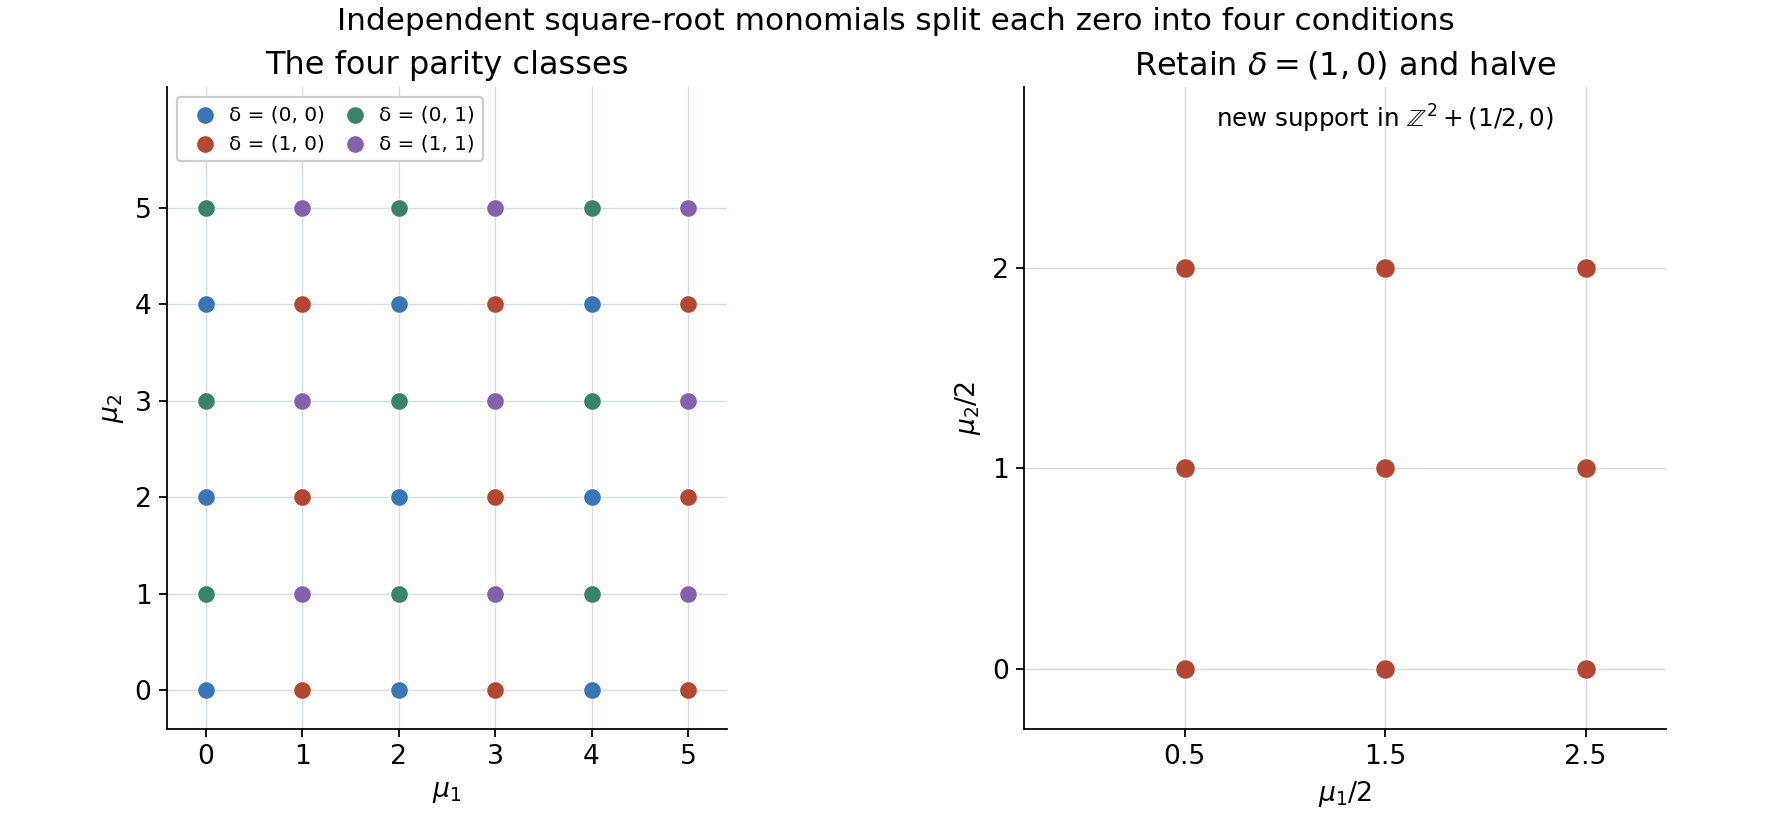
\includegraphics[keepaspectratio,alt={The four parity classes of a square exponent support and the retained half-support.}]{../figures/logarithmic-parity-division.png}}
\par\smallskip
\begin{flushleft}\small
\emph{Figure 8.1. The exact support \(\mathcal U=\{0,\ldots,5\}^2\)
splits into four classes. Selecting \(\delta=(1,0)\) and dividing the
exponents by two gives nine points of \(\mathbb Z^2+(1/2,0)\). Equation
(8.14) explains why every class inherits the odd-point zeros. This is an
exponent-support illustration; it does not assign numerical logarithms
to the axes. Source mechanism: {[}Matveev 2000{]}. Reproducible source:
\href{../figure_sources/logarithmic_lattice_geometry.py}{logarithmic\_lattice\_geometry.py}.}
\end{flushleft}
\end{minipage}\par\medskip


\subsubsection{Volume after imposing logarithmic
constraints}\label{volume-after-imposing-logarithmic-constraints}

Cutting a box by a few logarithmic constraints loses a power
corresponding to the number of constraints, rather than a power
corresponding to its full dimension. The needed convex-volume fact is as
follows.

\textbf{Lemma (Brunn--Minkowski for convex bodies).} If \(A,B\) are
compact convex bodies in \(\mathbb R^d\), then for \(0\le t\le1\), \[
\operatorname{vol}_d((1-t)A+tB)^{1/d}
\ge(1-t)\operatorname{vol}_d(A)^{1/d}
+t\operatorname{vol}_d(B)^{1/d}.
\tag{8.15}
\]

\textbf{Proof.} In dimension one this is the length identity for
intervals. Induct on \(d\), first assuming positive volumes and
normalizing them both to one. Slice \(A\) and \(B\) by their first
coordinate; write their \((d-1)\)-dimensional slice volumes as \(a(x)\)
and \(b(y)\). They are positive and continuous on the interiors of their
projection intervals: the induction hypothesis and convexity show that
their \(1/(d-1)\)-th powers are concave there, and a finite concave
function is continuous in an open interval. Let \(x(s),y(s)\),
\(0<s<1\), be the inverse cumulative slice volumes. Then \[
x'(s)=1/a(x(s)),\qquad y'(s)=1/b(y(s)).
\] At first coordinate \(z(s)=(1-t)x(s)+t y(s)\), the slice of
\((1-t)A+tB\) contains the Minkowski combination of the two slices. By
induction its volume is at least \[
\big((1-t)a(x(s))^{1/(d-1)}
+t b(y(s))^{1/(d-1)}\big)^{d-1}
\ge a(x(s))^{1-t}b(y(s))^t.
\] The last inequality is the weighted arithmetic-geometric mean
inequality. Also \[
z'(s)=\frac{1-t}{a(x(s))}+\frac{t}{b(y(s))}
\ge a(x(s))^{-(1-t)}b(y(s))^{-t}.
\] Integrating the product of these two lower bounds over \(0<s<1\)
shows that the Minkowski combination has volume at least one. All
substitutions can first be performed on
\(\varepsilon\le s\le1-\varepsilon\), where the functions are
continuously differentiable, and then extended by monotone convergence.

For arbitrary positive volumes put \(a_0=\operatorname{vol}(A)^{1/d}\),
\(b_0=\operatorname{vol}(B)^{1/d}\), \(c=(1-t)a_0+t b_0\), and
\(\theta=t b_0/c\). The combination in (8.15) is \[
c\big((1-\theta)(A/a_0)+\theta(B/b_0)\big).
\] Both normalized bodies have volume one, so scaling proves (8.15). If
a volume is zero, add a closed ball of radius \(\varepsilon\) to each
body, apply the positive-volume result, and let
\(\varepsilon\downarrow0\). These compact neighborhoods decrease to the
original bodies, so continuity of measure from above proves the
assertion. \(\square\)

\textbf{Lemma (volume of a clipped body).} Let \(W=-W\) be a compact
convex body in \(\mathbb R^r\), let \(T:\mathbb R^r\to U\) be a real
linear map of rank \(\rho\), and give \(U\) any norm. If
\(\sup_{w\in W}\|Tw\|\le Z\), then, for \(Y>0\), \[
\operatorname{vol}_r\{w\in W:\|Tw\|\le Y\}
\ge\operatorname{vol}_r(W)\max\{1,Z/Y\}^{-\rho}.
\tag{8.16}
\]

\textbf{Proof.} Only \(c=Z/Y>1\) requires proof. Write
\(\mathbb R^r=X\oplus\ker T\) orthogonally, with \(\dim X=\rho\). Let
\(f(x)\) be the volume of the fiber \(W\cap(x+\ker T)\). For positive
fiber dimension \(d\), convexity and (8.15) show that \(f^{1/d}\) is
concave on its support. Symmetry makes it even. On each line through
zero it is therefore nonincreasing in the positive radial direction: if
\(0\le s\le1\), write \(sx=((1+s)/2)x+((1-s)/2)(-x)\) and use concavity.
Thus \(f(x/c)\ge f(x)\). If the fiber dimension is zero, use the
indicator of \(W\), for which the same inequality follows from convexity
and \(0\in W\).

For every \(x\) in the projection of \(W\), \(\|Tx\|\le Z\), so
\(\|T(x/c)\|\le Y\). Integrating over these contracted projected points
gives \[
\operatorname{vol}_r(W\cap\{\|Tw\|\le Y\})
\ge c^{-\rho}\int f(x/c)\,dx
\ge c^{-\rho}\int f(x)\,dx.
\] This is (8.16). \(\square\)

\begin{minipage}[t]{\linewidth}
\centering
\pandocbounded{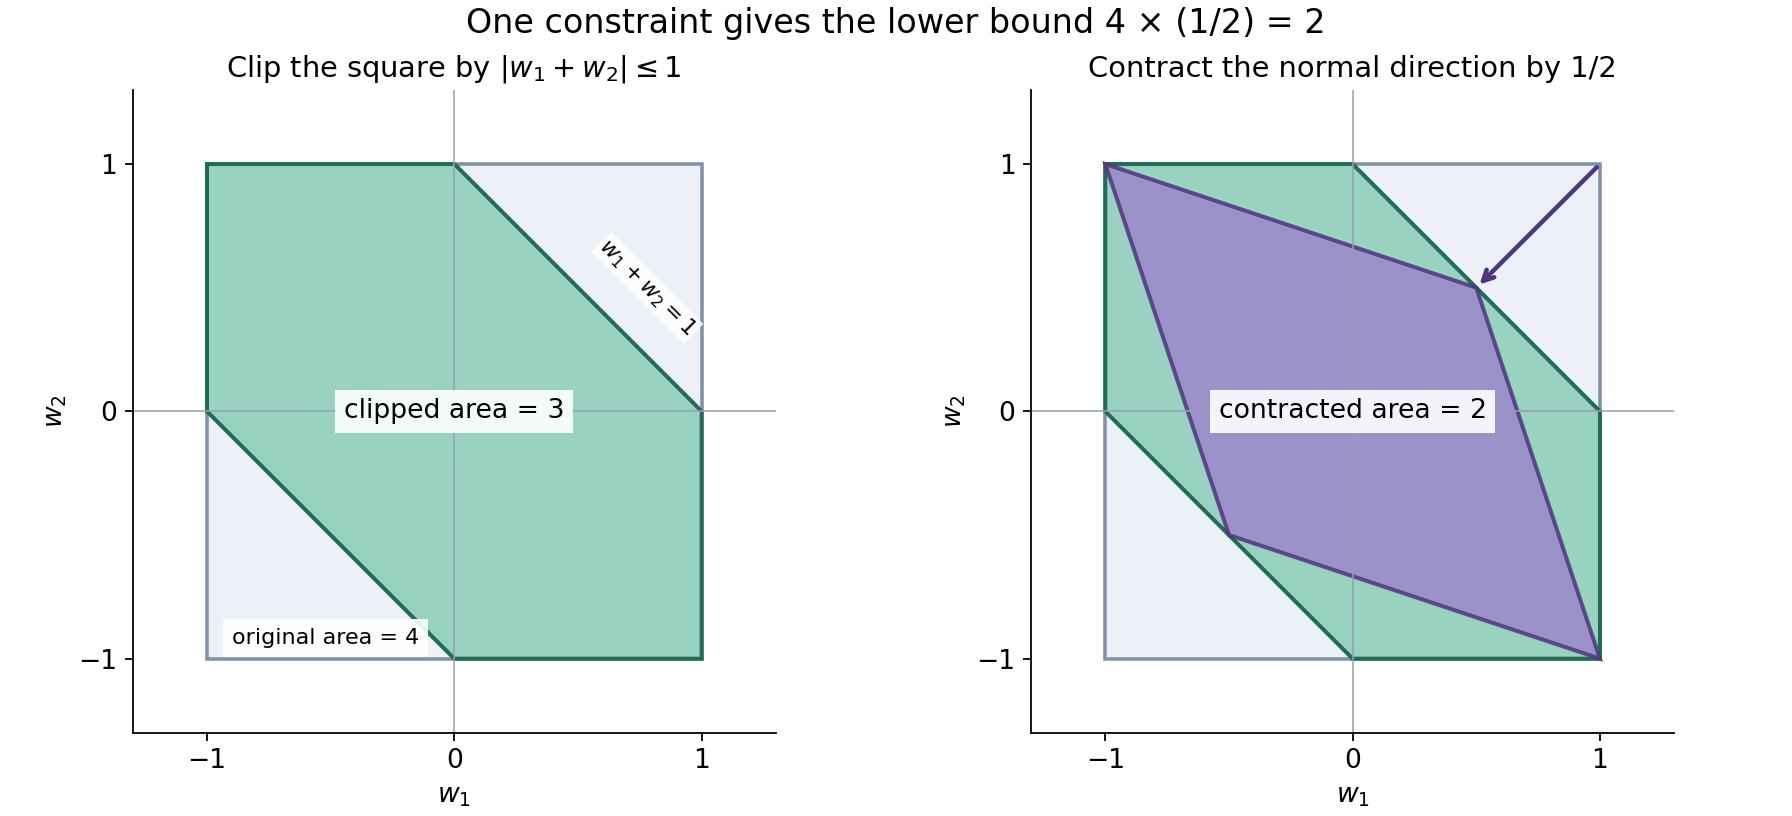
\includegraphics[keepaspectratio,alt={A square clipped by one linear constraint, with the exact area lower bound.}]{../figures/clipped-logarithmic-body.png}}
\par\smallskip
\begin{flushleft}\small
\emph{Figure 8.2. For \(W=[-1,1]^2\), \(T(w)=w_1+w_2\), \(Z=2\) and
\(Y=1\), the clipped area is \(3\). Lemma (8.16) proves the lower bound
\(4(1/2)^1=2\). In this symmetric square example, contraction by \(1/2\)
in the normal direction is the matrix
\(\bigl(\begin{smallmatrix}3/4&-1/4\\-1/4&3/4\end{smallmatrix}\bigr)\);
its image has area \(2\) and lies in the clipped hexagon. The general
proof uses fiber volumes, so it does not require every symmetric body to
contain this particular contracted image. Source mechanism: {[}Matveev
1999{]}. Reproducible source:
\href{../figure_sources/logarithmic_lattice_geometry.py}{logarithmic\_lattice\_geometry.py}.}
\end{flushleft}
\end{minipage}\par\medskip


\subsubsection{Counting small algebraic logarithmic
vectors}\label{counting-small-algebraic-logarithmic-vectors}

We use the coordinate description (8.11), replacing the selected real
coordinate and its imaginary coordinate by their complex combination.
For \(\kappa=2\), count the selected embedding and its conjugate, with
conjugate chosen logarithms. For \(\kappa=1\) in the following lattice
estimates, use positive bases and real logarithms in the specified real
embedding. Let \(S\) be this set of \(\kappa\) coordinates.

\textbf{Lemma (a determinant cardinality bound).} Suppose
\(x_1,\ldots,x_J\), \(J\ge2\), belong to one translate of the
logarithmic lattice, and their recovered algebraic bases are distinct.
At unselected coordinates suppose \(|x_{j,\sigma}|\le X_\sigma\), and at
selected coordinates suppose \(|z_{j,\sigma}|\le Y_\sigma\). If \[
\frac1{2\kappa}\sum_{\sigma\notin S}X_\sigma\le X,\qquad
\frac1\kappa\sum_{\sigma\in S}Y_\sigma\le Y,
\] then \[
\frac D\kappa\,\frac{\log J}{J-1}
+1+\frac{XJ}{J-1}
-\log\frac{2(J-1)}{JY}\ge0.
\tag{8.17}
\]

\textbf{Proof.} Write \(x_j=w+v(\alpha_j,\lambda_j)\), and put
\(a=(J-1)/2\). Consider the nonzero algebraic number \[
\Delta=
\left(\prod_{j=1}^J\alpha_j^{-(J-1)}\right)
\det(\alpha_j^k)_{0\le k<J,\ 1\le j\le J}^{\,2}.
\] It is nonzero because it equals a nonzero monomial times the
Vandermonde determinant in the distinct \(\alpha_j\). At a selected
embedding define the entire function \[
\Delta_\sigma(\zeta)=
\zeta^{-J(J-1)}
\det\big(\exp((k-a)\lambda_{j,\sigma}\zeta)\big)^2.
\] The apparent singularity at zero is removable. Expanding rows in
powers of \(\zeta\), a nonzero term uses distinct nonnegative exponents,
whose sum is at least \(0+1+\cdots+(J-1)\); squaring doubles that order.
At \(\zeta=1\), its absolute value is \(|\Delta|_\sigma\).

Since \(\sum_k(k-a)=0\), translating all coordinates by \(w\) introduces
factors whose product in the determinant is one. Also
\(\sum_k|k-a|\le J^2/4\). At each unselected place choose square roots
in an algebraic closure to write \(\Delta\) as the square of the
determinant with powers \(k-a\); its absolute value is independent of
their signs. The row-norm form of Hadamard, at an archimedean place, and
the ultrametric determinant bound, at a finite place, therefore give \[
|\Delta|_\sigma\le\gamma_\sigma
\exp(J^2X_\sigma/2)\quad(\sigma\notin S),
\] and \[
|\Delta_\sigma(\zeta)|\le
|\zeta|^{-J(J-1)}\gamma_\sigma
\exp(J^2Y_\sigma|\zeta|/2)\quad(\sigma\in S),
\] where \(\gamma_\sigma=J^J\) at an archimedean place and \(1\) at a
finite place. Form the analytic function \[
F(\zeta)=
\left(\prod_{\sigma\notin S}|\Delta|_\sigma\right)
\prod_{\sigma\in S}\Delta_\sigma(\zeta).
\] The product formula gives \(|F(1)|=1\), and on the circle
\(|\zeta|=R\), \[
\log|F(\zeta)|
\le DJ\log J+\kappa XJ^2
+\tfrac12\kappa YRJ^2-\kappa J(J-1)\log R.
\] If \(R=2(J-1)/(JY)>1\), apply the maximum modulus principle at \(1\),
substitute this radius and divide by \(\kappa J(J-1)\). This gives
(8.17). If that radius is at most one, the final logarithm in (8.17) is
nonpositive, so the assertion is immediate. \(\square\)

Here is the uniform numerical consequence used below. For every
\(\delta\ge1\), \(J\ge7\), and \(\eta\ge0\), the expression in (8.17),
with \[
X=\frac{n\eta}{2+\eta},\qquad
Y=\frac{e^{-X}}{2(2+\eta)},\qquad n\le J,
\] is negative if \(J\ge\delta\log(4.64\delta)\), where
\(\delta=D/\kappa\). Indeed it becomes \[
\delta\frac{\log J}{J-1}+1+
\frac{n\eta}{(J-1)(2+\eta)}
-\log\frac{4(2+\eta)(J-1)}J .
\] Enlarge \(n\) to \(J\). Differentiation shows that its maximum over
\(\eta\ge0\) occurs at \(\eta=2/(J-1)\), and equals \[
\left(1+\frac1{J-1}\right)
\left(1+\delta\frac{\log J}J\right)-\log8.
\tag{8.18}
\] For fixed \(J\), this increases with \(\delta\). Under the indicated
hypothesis, \(\delta\) is at most the solution \(\delta_0\) of
\(J=\delta_0\log(4.64\delta_0)\). Put \(t=\log(4.64\delta_0)\), so
\(J=t e^t/4.64\). Then (8.18) is \[
\left(1+\frac1{t e^t/4.64-1}\right)
\left(2+\frac{\log(t/4.64)}t\right)-\log8<0.
\tag{8.19}
\] The last strict inequality has a reproducible rational interval
certificate,
\href{../verification/logarithmic_lattice.py}{logarithmic\_lattice.py}.
Since \((127/50)e^{127/50}/4.64<7\), every \(J\ge7\) has \(t>127/50\).
The certificate covers \(127/50\le t\le13\) by 1,046 intervals of width
\(1/100\); their largest certified upper bound is less than
\(-0.0000916\). For \(t\ge13\), the factor \(1+1/(t e^t/4.64-1)\)
decreases, and \(\log(t/4.64)/t\le1/(4.64e)\). The resulting tail bound
is less than \(-0.0001555\). Every computation uses outward rational
intervals and explicit exponential and logarithmic series tails, so no
rounded decimal is used to certify the assertion.

\textbf{Proposition (product and index of logarithmic vectors).} Let
\(v_1,\ldots,v_n\) be real-linearly independent extended logarithmic
vectors, let \(M\) be the saturated lattice in their span, and let
\(N=[M:\sum_j\mathbb Z v_j]\). For \(\theta>0\) put \[
V_j=\max\left\{|\lambda_j|,
\frac{\theta}{2\kappa}\sum_{\sigma\notin S}|v_{j,\sigma}|\right\},\qquad
C=2+\frac1{2\theta}.
\] Then \[
N\le
\left(\prod_{j=1}^nV_j\right)
C^n\bigl(n e^{\,n/(1+4\theta)}\bigr)^\kappa
\max\{6,n-1,(D/\kappa)\log(4.64D/\kappa)\}.
\tag{8.20}
\]

\textbf{Proof.} In coordinates relative to the \(v_j\), the saturated
lattice has covolume \(1/N\): the sublattice with those vectors as basis
has covolume one and index \(N\). Put \[
W=\{w\in\mathbb R^n:|w_j|\le1/(2CV_j)\},\quad
X=\frac{n}{1+4\theta},\quad Y=\frac{e^{-X}}{2C}.
\] Clip \(W\) by the selected logarithmic conditions
\(|\sum_jw_j\lambda_{j,\sigma}|\le Y\). Their real rank is at most
\(\kappa\): one real functional in the real case, or the real and
imaginary parts of one complex functional in the complex case. On the
full box their norms are at most \(Z=n/(2C)\). Lemma (8.16) therefore
gives \[
\operatorname{vol}_n(W_{\rm clipped})
\ge\frac{(n e^X)^{-\kappa}}{C^n\prod V_j}.
\tag{8.21}
\]

Integrate the number of points of \(W_{\rm clipped}\) in each lattice
coset over a fundamental domain. Its average is
\(N\operatorname{vol}(W_{\rm clipped})\); hence some coset contains an
integer number \(J\) of points at least that large. This is the counting
form of Blichfeldt's argument, with its full averaging calculation.
Their images in logarithmic space satisfy the unselected bound \[
\frac1{2\kappa}\sum_{\sigma\notin S}
\max_{w\in W}\left|\sum_jw_jv_{j,\sigma}\right|
\le\sum_j\frac1{2CV_j}\frac{V_j}{\theta}
=\frac n{2C\theta}=X,
\] and the selected bound \(Y\). Two of their recovered bases cannot be
equal: their selected logarithms would differ by a nonzero period of
modulus at least \(2\pi\), whereas their difference has modulus at most
\(2Y<2\pi\). Thus the determinant bound applies whenever \(J\ge2\).

If \(J\) were larger than all three entries of the maximum in (8.20),
then \(J\ge7\), \(J\ge n\), and \(J>\delta\log(4.64\delta)\),
contradicting (8.17) and (8.19). It follows that \(J\) is at most that
maximum. Combine this with its lower bound and (8.21) to prove (8.20).
\(\square\)

In particular, with \(\theta=\kappa\) and cutoffs
\(A_j\ge\max\{D h(\alpha_j),|\lambda_j|\}\), we have \(V_j\le A_j\). For
\(n\ge2\), (8.20) gives \[
A_1\cdots A_n\,\frac{3.1^n n^\kappa}{\kappa}\,
D\log(e^{n+4}D)>N.
\tag{8.22}
\] To check the simplification, note \[
C e^{\kappa/(1+4\kappa)}<3.1
\quad(\kappa=1,2),
\] which the same certificate verifies. Also each of \(6\), \(n-1\) and
\((D/\kappa)\log(4.64D/\kappa)\) is at most
\((D/\kappa)\log(e^{n+4}D)\), since \(D/\kappa\ge1\), \(n\ge2\). The
strict inequality in the exponential base gives the strictness in
(8.22).

This supplies the product-index estimate of {[}Matveev 1999{]} and
{[}Matveev 2000{]}, for every \(n\ge2\), together with its convex-volume
and arithmetic determinant proofs.

\subsubsection{The one-vector height
estimate}\label{the-one-vector-height-estimate}

The preceding product estimate treats at least two independent vectors.
A sharper use of the Vandermonde product treats one vector.

\textbf{Lemma (extended height of one algebraic number).} Let
\(\alpha\ne0\) have degree \(d\ge2\), and let \(\lambda\ne0\) be any
logarithm of \(\alpha\). Then \[
\max\{d h(\alpha),|\lambda|\}>
\frac8{9d\log(2.2d)}.
\tag{8.23}
\] Consequently, for every degree-\(D\) field containing \(\alpha\), and
every cutoff \(A\ge\max\{D h(\alpha),|\lambda|\}\), \[
\frac1A<1.5D\log(eD).
\tag{8.24}
\]

\textbf{Proof.} Work first in \(F=\mathbb Q(\alpha)\), and put
\(L=\log(2.2d)\). Suppose \(A=\max\{d h(\alpha),|\lambda|\}\le8/(9dL)\).
For \(d\ge3\), choose \[
m=\left\lceil\tfrac45 dL\right\rceil.
\] The numbers \(1,\alpha,\ldots,\alpha^{m-1}\) are distinct. This is
immediate unless \(\alpha\) is a root of unity of order \(q\). In that
case a nonzero chosen logarithm has modulus at least \(2\pi/q\), while
\[
m|\lambda|\le mA\le\tfrac{32}{45}+\frac8{9dL}<2\pi;
\] hence \(q>m\).

Put \(a=(m-1)/2\), and consider the centered determinant \[
\mathcal D=\det(\exp((j-a)(k-a)\lambda))_{0\le j,k<m}.
\] Its fourth power is a nonzero element of \(F\): expanding the
determinant gives monomials with exponents whose denominators divide
four, and the centering differs from the ordinary Vandermonde by a
single such monomial. Thus the product formula applies to its local
absolute values.

At the specified embedding the exact Vandermonde identity gives \[
\mathcal D=\prod_{0\le j<k<m}2\sinh((k-j)\lambda/2).
\] The integral representation of \(\sinh\) gives \[
|2\sinh(t\lambda/2)|\le t|\lambda|e^{t|\operatorname{Re}\lambda|/2}
\qquad(t\ge1).
\] It follows that \[
\log|\mathcal D|
\le\tfrac12m(m-1)\log|\lambda|
+\sum_{t=1}^{m-1}(m-t)\log t
+\tfrac1{12}m(m^2-1)|\operatorname{Re}\lambda|.
\tag{8.25}
\] At every other embedding, Hadamard gives \[
\log|\mathcal D|_\sigma
\le\tfrac m2\log m+
\tfrac18m^2(m-1)|\log|\alpha|_\sigma|.
\] At a finite place the same bound holds without the first term, by the
ultrametric determinant inequality. If the specified embedding is
complex, its conjugate has the bound (8.25) as well. Write \(\kappa=1\)
or \(2\) for the number of these embeddings. The sum of the remaining
absolute logarithms is
\(2d h(\alpha)-\kappa|\operatorname{Re}\lambda|\). The terms multiplying
\(\kappa|\operatorname{Re}\lambda|\), after combining the bounds, have
coefficient \[
\tfrac1{12}m(m^2-1)-\tfrac18m^2(m-1)
=-\tfrac1{24}m(m-1)(m-2)\le0.
\] Discard them. The product formula therefore yields \[
0\le
\frac{d-\kappa}{\kappa}\frac{\log m}{m-1}
+\frac{d h(\alpha)}{\kappa}\frac m2
+\log|\lambda|
+\frac2{m(m-1)}\sum_{t=1}^{m-1}(m-t)\log t.
\tag{8.26}
\]

The function \((m-x)\log x\) is concave on \([1,m]\), and is zero at
both endpoints. Its integral is therefore at least its trapezoidal sum:
\[
\sum_{t=1}^{m-1}(m-t)\log t
\le \frac{m^2}2\log m-\frac{3m^2}4+m-\frac14.
\] Use this in (8.26), enlarge \(d h(\alpha)\) and \(|\lambda|\) to
\(A\), and take the larger value \(\kappa=1\) in the resulting positive
degree terms. We obtain \[
0\le d\frac{\log m}{m-1}
+\frac{4m}{9dL}+\log\frac{8m}{9dL}
-\frac32+\frac1{2m}.
\tag{8.27}
\]

This right side is strictly negative for every \(d\ge3\). For
\(3\le d\le99\),
\href{../verification/logarithmic_lattice.py}{logarithmic\_lattice.py}
computes \(L\) by outward rational intervals, certifies the single
integer value of \(m\), and bounds (8.27); its largest upper bound is
less than \(-0.04236\). For \(d\ge100\), \(L>5\) and \[
\frac m{dL}\le\frac45+\frac1{dL}\le\frac{401}{500}.
\] Also, using \(\log(1+u)\le u\) and \(\log(x/a)\le x/(ae)\) for
\(x>0\), \[
d\frac{\log m}{m-1}
\le\frac{L+\log(4L/11)+1/(80L)}{(4/5)L-1/100}
\le
\frac{1+4/(11e)+1/2000}{399/500}<\frac{143}{100}.
\] Here \(m\le(4/5)dL+1\), \(m-1\ge(4/5)dL-1\), and \(e>27/10\) justify
each bound. Since \(m\ge400\), put \(q=802/1125<1\) and use
\(\log q\le(q-1)-(q-1)^2/2\). The right side of (8.27) is at most \[
\frac{143}{100}
+\frac49\frac{401}{500}
+(q-1)-\frac{(q-1)^2}{2}
-\frac32+\frac1{800}
=-\frac{1645639}{40500000}<0.
\] This contradiction proves (8.23) for \(d\ge3\).

For \(d=2\), a nonintegral number, or an integral nonunit, has
\(2h(\alpha)\ge\log2\). For a quadratic unit with real conjugates and
not a root of unity, write its minimal polynomial as
\(X^2-tX+\varepsilon\), \(t\in\mathbb Z\), \(\varepsilon=\pm1\). If
\(\varepsilon=-1\), then \(|t|\ge1\) unless the polynomial is reducible,
so the larger root modulus is at least \((1+\sqrt5)/2\). If
\(\varepsilon=1\), the real non-torsion case has \(|t|\ge3\), giving a
still larger root modulus. Thus \(2h(\alpha)\ge\log((1+\sqrt5)/2)\). A
quadratic unit with nonreal conjugates has both moduli one, hence height
zero and is a root of unity by Theorem 8.3. In the torsion case its
order is at most \(2d^2=8\), so \(|\lambda|\ge\pi/4\). Every one of
these bounds exceeds \(8/(18\log4.4)\), as follows directly from the
rational interval arithmetic in the same certificate.

To deduce (8.24), \(D\ge d\) and \(2.2<e\) give \[
A>\frac8{9D\log(2.2D)}
>\frac2{3D\log(eD)}
\quad(d\ge2).
\] If \(\alpha\) is rational and different from \(1,-1\), then
\(h(\alpha)\ge\log2>2/3\). If it is \(1\) or \(-1\), a nonzero logarithm
has modulus at least \(\pi>2/3\). These facts also prove (8.24) for
degree-one bases. \(\square\)

This establishes the one-vector estimate used in {[}Matveev 2000{]}, by
a complete Vandermonde calculation and a reproducible uniform
certificate.

\subsubsection{Euclidean covolumes of logarithmic
lattices}\label{euclidean-covolumes-of-logarithmic-lattices}

In the coordinate space (8.11) use \[
\|v\|_2^2=\sum_{\sigma\ {\rm archimedean}}x_\sigma^2
+\sum_{\mathfrak p}x_{\mathfrak p}^2
+(\operatorname{Im}\lambda)^2.
\] The last term is absent for positive bases with real logarithms. Let
\(k=1\) when it is present and \(k=0\) otherwise. Extend the height norm
to all real vectors of this coordinate space by \[
\mathcal H(v)=
\max\left\{\tfrac12\sum_{\text{archimedean and finite coordinates}}|v_j|,
\,|x_{\rm selected}+i y|\right\}.
\] All these real vectors satisfy the additive product formula. On
algebraic logarithmic vectors this norm is
\(\max\{D h(\alpha),|\lambda|\}\).

\textbf{Lemma (covolume bounds).} Let \(M\) be an \(r\)-dimensional
lattice of extended logarithmic vectors in a degree-\(D\) field,
\(D\ge2\). Put \[
R_D=\frac8{9D^{3/2}\log(eD)}.
\] Then \[
\operatorname{covol}_r(M)\ge
\frac{\pi^{r/2}}{\Gamma(1+r/2)}R_D^r.
\tag{8.28}
\] Also, if \(B_r\) is the supremum of the Euclidean volume of
parallelepipeds spanned by arbitrary real vectors \(v_1,\ldots,v_r\) in
this coordinate space satisfying \(\mathcal H(v_j)\le1\), then \[
B_r\le(k+2)^{r/2}.
\tag{8.29}
\] For \(K=\mathbb Q\), let \(P_1\le P_2\le\cdots\) be the increasing
list of the prime logarithms together with \(\pi\) when imaginary
coordinates are allowed. Then \[
\operatorname{covol}_r(M)\ge P_1\cdots P_r.
\tag{8.30}
\] In the positive rational case omit \(\pi\).

\textbf{Proof.} We first show that no nonzero logarithmic vector has
Euclidean length less than \(2R_D\). Since \(2R_D<\log2\), all its
finite coordinates would have to vanish: a nonzero prime valuation has
modulus at least \(\log N\mathfrak p\ge\log2\). Its base would therefore
be a unit.

For \(D\ge4\), Cauchy--Schwarz and the height formula give \[
D h(\alpha)=\tfrac12\sum_{\sigma}|x_\sigma|
\le\tfrac{\sqrt D}{2}\|v\|_2<R_D\sqrt D,
\qquad
|\lambda|\le\|v\|_2<2R_D\le R_D\sqrt D.
\] But \(R_D\sqrt D=8/(9D\log(eD))\) is strictly smaller than the
one-vector lower bound (8.23), with the actual degree of the base or the
rational exceptions treated in (8.24). This is a contradiction.

For \(D=2\), a nontorsion unit has some conjugate with logarithmic
modulus at least \(\log((1+\sqrt5)/2)>2R_2\), by the quadratic argument
above. For \(D=3\), a unit of actual degree three has a monic
irreducible polynomial \[
X^3+aX^2+bX+c,\qquad a,b\in\mathbb Z,\quad c=\pm1.
\] If all conjugate moduli lay strictly between \(5/6\) and \(6/5\),
then \(|a|<18/5\). The product of the roots has modulus one, so the
pairwise products have moduli equal to the reciprocals of the root
moduli; hence \(|b|<18/5\) as well. Replacing the base by its negative
if needed reduces to \(c=1\), with \(-3\le a,b\le3\). Irreducibility
excludes \(a+b=-2\) and \(a=b\), since these are precisely the cases of
roots \(1\) and \(-1\).

There are 38 remaining pairs. The exact finite check in
\href{../verification/logarithmic_lattice.py}{logarithmic\_lattice.py}
evaluates \(f(6/5),f(-6/5),f(5/6),f(-5/6)\) for each. Either
\(f(6/5)\le0\), giving a real root at least \(6/5\); or \(f(-6/5)\ge0\),
giving a real root at most \(-6/5\); or the two inner values have
opposite signs, giving a real root in \([-5/6,5/6]\). All comparisons
are rational, and the certificate records the pair and its excluding
case. Thus no irreducible cubic unit has all its conjugate moduli in the
indicated interval. Since \(2R_3<\log(6/5)\), a vector of length less
than \(2R_3\) would contradict this check. A degree-one unit is \(1\) or
\(-1\), and cannot supply a nonzero vector this small.

For torsion bases in these two field degrees, the order bound gives a
nonzero logarithm of modulus at least \(\pi/4\) for \(D=2\), or
\(\pi/9\) for \(D=3\). Both exceed \(2R_D\). The certificate also checks
all the numerical comparisons used in these small-degree cases.

Intersect the open ball of radius \(2R_D\) with the real span of \(M\).
It contains no nonzero lattice point. Minkowski's theorem therefore
gives \[
\operatorname{vol}_r(\text{ball of radius }2R_D)
\le2^r\operatorname{covol}_r(M),
\] which is (8.28). The formula for the unit-ball volume follows by
integrating \(e^{-\|x\|^2}\): the product of the one-dimensional
Gaussian integrals is \(\pi^{r/2}\), while radial integration gives
\(\operatorname{vol}(\mathbb B_r)\Gamma(1+r/2)\), where \(\mathbb B_r\)
denotes the Euclidean unit ball. This also defines the gamma function
for the half-integer values appearing here.

For (8.29), the additive product formula makes the sum of the positive
real coordinates, including both archimedean and finite coordinates,
equal to the absolute sum of the negative ones. Both sums are at most
one on the continuous height-norm unit ball. Thus \[
\sum_{\text{real coordinates }j} x_j^2
\le\left(\sum_{x_j>0}x_j\right)^2
+\left(\sum_{x_j<0}x_j\right)^2\le2.
\] The possible imaginary coordinate has modulus at most one. Each
Euclidean vector length is therefore at most \(\sqrt{k+2}\); Hadamard
proves (8.29).

Finally consider a lattice of rational bases. Its finite coordinates are
integer multiples of \(\log p\), and its imaginary coordinate, when
present, is an integer multiple of \(\pi\). Project away the real
archimedean coordinate. This projection is injective on logarithmic
vectors: the prime exponents and the integer period recover the signed
rational base and its logarithm. For any integer basis of \(M\), its
projected matrix is an integer matrix multiplied row by row by the
corresponding numbers \(\log p\), or \(\pi\). It has rank \(r\).
Cauchy--Binet expresses the squared projected covolume as the sum of
squares of its \(r\)-row minors. Some integer minor is nonzero and has
absolute value at least one, and its product of row weights is at least
\(P_1\cdots P_r\). Projection cannot increase volume, again by
Cauchy--Binet after including the discarded row. This proves (8.30),
without a cube-section theorem. \(\square\)

The ratio needed for integer relations consequently has one formula for
\(D\ge2\) and for positive rational bases: \[
\frac{B_r}{\operatorname{covol}_r(M)}
\le
2.2\,\Gamma(1+r/2)
\left(\frac3\pi\right)^{r/2}
\left(\frac98D^{3/2}\log(eD)\right)^r.
\tag{8.31}
\] For \(D\ge2\), (8.28)--(8.29) prove this even with the factor \(2.2\)
replaced by one. For positive rational bases, (8.30) and
\(B_r\le2^{r/2}\) reduce the assertion to an explicit inequality
involving the first \(r\) prime logarithms. The exact interval
certificate
\href{../verification/logarithmic_lattice.py}{logarithmic\_lattice.py}
checks \(r=1,2,3\). To cover every larger dimension, let \(F_r\) be the
ratio of \(2^{r/2}/\prod_{j\le r}\log p_j\) to the right side of (8.31)
with \(D=1\). The gamma recurrence gives \[
\frac{F_{r+2}}{F_r}
=\frac{256\pi}
{243(r+2)\log p_{r+1}\log p_{r+2}}<1
\qquad(r\ge2).
\] Indeed, both prime logarithms exceed one, and \(256\pi<972\), as
certified by the same rational interval for \(\pi\). Induction on each
parity proves (8.31) in every dimension. The rational case here concerns
positive bases with real logarithms, which is the case used after the
real-embedding reduction.

\subsubsection{The discriminant of the coefficient
field}\label{the-discriminant-of-the-coefficient-field}

The height of a generating set controls the discriminant without first
choosing a primitive element of large height.

\textbf{Lemma (discriminant and generators).} If
\(K=\mathbb Q(\alpha_1,\ldots,\alpha_n)\), \([K:\mathbb Q]=D\), then \[
\log|\Delta_K|
\le D\log D+2D(D-1)\max_j h(\alpha_j).
\tag{8.32}
\] More precisely, write \(K_j=\mathbb Q(\alpha_1,\ldots,\alpha_j)\),
\(K_0=\mathbb Q\), and \(d_j=[K_j:K_{j-1}]\). Then \[
\frac{\log|\Delta_K|}{D}
\le \log D+2\sum_j(d_j-1)h(\alpha_j).
\tag{8.33}
\]

\textbf{Proof.} We first prove the relative bound for \(L=F(\alpha)\),
with \(e=[L:F]\ge2\). Let \[
q(X)=X^e+c_1X^{e-1}+\cdots+c_e\in F[X]
\] be the minimal polynomial. At a finite place \(v\) of \(F\), use the
absolute value extending the ordinary \(p\)-adic absolute value, and put
\[
H_v(q)=\max\{1,|c_1|_v,\ldots,|c_e|_v\}.
\] Choose \(a_0\in F_v^\times\) with \(|a_0|_v=H_v(q)^{-1}\). This is
possible because the maximum is a value of a coefficient in \(F_v\). All
coefficients \(a_i=a_0c_i\) of \(f=a_0q\), with \(c_0=1\), then lie in
the valuation ring.

For \(1\le k<e\) set \[
\beta_k=a_0\alpha^k+a_1\alpha^{k-1}+\cdots+a_{k-1}\alpha.
\] These elements are integral at every place of \(L\) above \(v\). For
a conjugate \(\alpha'\) with \(|\alpha'|_v\le1\), this follows from the
displayed expression. For \(|\alpha'|_v>1\), the equation
\(f(\alpha')=0\) gives instead \[
\beta_k'=-a_k-a_{k+1}(\alpha')^{-1}
-\cdots-a_e(\alpha')^{k-e},
\] whose absolute value is again at most one. A root whose every local
conjugate has absolute value at most one is integral: the elementary
symmetric functions of these conjugates are the coefficients of a monic
polynomial and belong to the valuation ring.

The vectors \(1,\beta_1,\ldots,\beta_{e-1}\) form an \(F_v\)-basis of
\(L\otimes_F F_v\); their change-of-basis matrix from
\(1,\alpha,\ldots,\alpha^{e-1}\) is triangular with determinant
\(a_0^{e-1}\). They span a submodule of the local ring of integers. The
trace discriminant of this submodule therefore has valuation at least
that of the relative field discriminant \(\mathfrak d_{L/F}\). To see
this directly, choose an integral basis locally over the discrete
valuation ring and write the displayed vectors in it. The coefficients
form an integral matrix, and the trace matrix changes as
\(T^{\mathsf t}AT\); its determinant is multiplied by \((\det T)^2\).
Consequently \[
|\mathfrak d_{L/F}|_v
\ge |a_0|_v^{2e-2}|\operatorname{disc}q|_v
 =H_v(q)^{-(2e-2)}|\operatorname{disc}q|_v.
\tag{8.34}
\]

Here, at a finite place \(v\) above \(p\) of ramification index \(e_v\),
the absolute value of an ideal of valuation \(t\) means \(p^{-t/e_v}\).
With weight \(n_v=[F_v:\mathbb Q_p]\), the product of the inverse
absolute values of an ideal is its absolute norm. Thus (8.34) and the
product formula for the nonzero number \(\operatorname{disc}q\) give \[
\log N_{F/\mathbb Q}\mathfrak d_{L/F}
\le
\sum_{v\mid\infty}n_v\log|\operatorname{disc}q|_v
+(2e-2)\sum_{v\nmid\infty}n_v\log H_v(q).
\tag{8.35}
\]

At an archimedean place, let \(\alpha'_1,\ldots,\alpha'_e\) be the roots
of \(q\), and put \(M_v(q)=\prod_i\max\{1,|\alpha'_i|_v\}\). The
Vandermonde matrix with rows \((1,\alpha'_i,\ldots,(\alpha'_i)^{e-1})\)
has row norm at most \(\sqrt e\,\max\{1,|\alpha'_i|_v\}^{e-1}\).
Hadamard therefore gives \[
|\operatorname{disc}q|_v\le e^e M_v(q)^{2e-2}.
\tag{8.36}
\] At a finite place, \[
H_v(q)=\prod_i\max\{1,|\alpha'_i|_v\}.
\tag{8.37}
\] For completeness, the coefficient maximum norm is multiplicative for
polynomials over a valued field: after scaling both polynomials to have
maximum one, their nonzero reductions have a nonzero product in the
residue-field polynomial ring. Factor \(q\) over a splitting field and
apply this fact to its linear factors. This proves (8.37), including
roots with fractional valuations.

The local degree formula for the conjugates now identifies \[
\sum_{v\mid\infty}n_v\log M_v(q)
+\sum_{v\nmid\infty}n_v\log H_v(q)
=[L:\mathbb Q]h(\alpha).
\] Indeed, each archimedean embedding of \(F\) has \(e\) extensions, and
at a finite place each place \(w\) of \(L\) contributes \([L_w:F_v]\)
conjugates, with \(n_v[L_w:F_v]=[L_w:\mathbb Q_p]\). Combining this
identity with (8.35)--(8.36) gives \[
\log N_{F/\mathbb Q}\mathfrak d_{L/F}
\le [L:\mathbb Q]\log e+
2(e-1)[L:\mathbb Q]h(\alpha).
\tag{8.38}
\]

The discriminant identity in a tower is \[
|\Delta_L|=|\Delta_F|^e
N_{F/\mathbb Q}\mathfrak d_{L/F}.
\tag{8.39}
\] It can be checked by the same trace-matrix calculation locally.
Choose a local integral basis \(\omega_i\) for \(F/\mathbb Q\) and
\(\eta_j\) for \(L/F\). The matrix of the conjugates of the products
\(\omega_i\eta_j\) factors into the matrix of the conjugates of the
\(\omega_i\), repeated \(e\) times, and the relative conjugate matrices
of the \(\eta_j\). Squaring the determinant gives the first factor
\(\Delta_F^e\) and the second factor equal to the norm of the relative
discriminant. The local bases span the full rings of integers, so there
is no index factor. Equality at every prime proves (8.39) for the
absolute ideal norms, irrespective of whether a global relative integral
basis exists.

Divide (8.39) by \([L:\mathbb Q]\) on the logarithmic scale and use
(8.38). Iterate along \(K_0\subseteq K_1\subseteq\cdots\subseteq K_n\),
omitting steps of degree one. Since \(\prod d_j=D\), this proves (8.33).
Finally \[
\sum_j(d_j-1)\le\prod_jd_j-1=D-1,
\] by repeated use of \((a-1)+(b-1)\le ab-1\) for integers \(a,b\ge1\).
Formula (8.32) follows. \(\square\)

This proves the discriminant bridge of {[}Matveev 2000{]}, including
nonintegral generators; replacing a nonintegral generator by an
arbitrary denominator-clearing multiple would lose the stated constant.

\subsubsection{Small solutions over the coefficient
field}\label{small-solutions-over-the-coefficient-field}

The auxiliary coefficients will satisfy linear equations over \(K\).
Their sizes must be controlled with different weights at the embeddings,
while allowing fractional-ideal conditions at the finite places. We
prove the required weighted Siegel lemma directly from Minkowski's
theorem and the ideal-lattice covolume formula of
\href{../../NT-ANT/lattices-minkowskis-theorem-and-the-minkowski-embedding.html}{\emph{Lattices,
Minkowski's theorem and the Minkowski embedding}}, Theorem 7.1 and
Proposition 7.2.

Use all \(D\) archimedean embeddings, counting a complex pair twice. For
a finite place indexed by \(\mathfrak p\), use
\(|a|_{\mathfrak p}=(N\mathfrak p)^{-v_{\mathfrak p}(a)}\); with these
conventions the product formula has no additional weights. Choose
positive \(q_{j,\sigma}\), equal at conjugate embeddings, and put \[
q_{j,\mathfrak p}=(N\mathfrak p)^{l_{j,\mathfrak p}},
\qquad l_{j,\mathfrak p}\in\mathbb Z,
\] with only finitely many \(l_{j,\mathfrak p}\ne0\). For
\(p,a\in K^J\), define \[
\begin{aligned}
L_\sigma(p)&=
\left(\sum_{j=1}^J|p_j|_\sigma^2/q_{j,\sigma}^2\right)^{1/2},
&
L_\sigma^*(a)&=
\left(\sum_{j=1}^J|a_j|_\sigma^2q_{j,\sigma}^2\right)^{1/2}
\quad(\sigma\mid\infty),\\
L_{\mathfrak p}(p)&=\max_j |p_j|_{\mathfrak p}/q_{j,\mathfrak p},
&
L_{\mathfrak p}^*(a)&=\max_j |a_j|_{\mathfrak p}q_{j,\mathfrak p}.
\end{aligned}
\] Let \[
\mathcal L(p)=\left(\prod_\sigma L_\sigma(p)\right)^{1/D},
\quad
\mathcal L^*(a)=\left(\prod_\sigma L_\sigma^*(a)\right)^{1/D},
\quad
q=\left(\prod_{j,\sigma}q_{j,\sigma}\right)^{1/(DJ)}.
\] The products range over the archimedean and finite places just
described.

\textbf{Lemma (weighted Siegel).} Let \(I<J\), and let
\(a_1,\ldots,a_I\in K^J\) be the rows of a homogeneous linear system.
There is a nonzero \(p\in K^J\) with \(a_i\cdot p=0\) for every \(i\),
and \[
\mathcal L(p)\le
\sqrt J\,|\Delta_K|^{1/(2D)}
\left(q^{-J}\prod_{i=1}^I
\max\{q,\mathcal L^*(a_i)\}\right)^{1/(J-I)}.
\tag{8.40}
\] The solution may be chosen with \(L_{\mathfrak p}(p)\le1\) at every
finite place. In particular, when all finite weights are one, all its
coordinates are algebraic integers.

\textbf{Proof.} First suppose that the \(I=r\) rows are \(K\)-linearly
independent, and put \(s=J-r\). Let \[
\mathfrak a_j=\prod_{\mathfrak p}\mathfrak p^{-l_{j,\mathfrak p}},
\qquad
\Gamma=\mathfrak a_1\oplus\cdots\oplus\mathfrak a_J.
\] Membership in \(\Gamma\) is precisely the collection of finite
conditions \(L_{\mathfrak p}(p)\le1\). Embed \(K^J\) in its archimedean
real space. At a real embedding use coordinates
\(p_j^\sigma/q_{j,\sigma}\); at each complex embedding use the real and
imaginary coordinates multiplied by \(\sqrt2/q_{j,\sigma}\). This metric
has squared length \(\sum_{\sigma\mid\infty} L_\sigma(p)^2\), with both
conjugate embeddings counted.

Proposition 7.2 gives the unweighted covolume
\(\sqrt{|\Delta_K|}\,N\mathfrak a\) for an ideal in this metric: its
factor \(2^{-r_2}\) is canceled by the \(\sqrt2\) in the two coordinates
of each complex pair. Scaling by the archimedean weights consequently
gives \[
\operatorname{covol}(\Gamma)
=|\Delta_K|^{J/2}
\left(\prod_{j,\sigma}q_{j,\sigma}\right)^{-1}
=|\Delta_K|^{J/2}q^{-DJ}.
\tag{8.41}
\] Here \(N\mathfrak a_j=\prod_{\mathfrak p}q_{j,\mathfrak p}^{-1}\)
accounts for the finite weights.

Let \(A:K^J\to K^r\) have rows \(a_i\), and give the target the
unweighted archimedean metric, again with the \(\sqrt2\) convention. At
a finite place write \[
L_{\mathfrak p}^*(a_i)=(N\mathfrak p)^{k_{i,\mathfrak p}},
\qquad
\mathfrak b_i=\prod_{\mathfrak p}\mathfrak p^{-k_{i,\mathfrak p}}.
\] The ultrametric inequality shows that \[
A\Gamma\subseteq\mathfrak b_1\oplus\cdots\oplus\mathfrak b_r.
\] Since \(A\) has rank \(r\), its image spans \(K^r\). More explicitly,
choose a \(K\)-linear right inverse of \(A\) and clear its finitely many
ideal denominators. For some nonzero integer \(c\), this gives
\(c\mathcal O_K^r\subseteq A\Gamma\). The image is a finitely generated
subgroup of the displayed ideal lattice and contains a full lattice, so
it is itself a full lattice. The inclusion has positive integer index.
Hence \[
\operatorname{covol}(A\Gamma)\ge
|\Delta_K|^{r/2}
\left(\prod_{\mathfrak p}\prod_{i=1}^r
L_{\mathfrak p}^*(a_i)\right)^{-1}.
\tag{8.42}
\]

Let \(\Gamma_0=\Gamma\cap\ker A\). It is a lattice of real dimension
\(Ds\): choose a \(K\)-basis of \(\ker A\), clear its finitely many
ideal denominators, and multiply each basis vector by an integral basis
of \(K\). These \(Ds\) independent real vectors lie in \(\Gamma_0\),
while the inclusion in \(\Gamma\) proves discreteness. Let
\(\mathcal J(A)\) be the product of the nonzero singular values of the
induced real linear map. The lattice volume identity is \[
\operatorname{covol}(\Gamma_0)=
\frac{\operatorname{covol}(\Gamma)\mathcal J(A)}
{\operatorname{covol}(A\Gamma)}.
\tag{8.43}
\] To prove it, choose an integer basis of \(A\Gamma\) and lift its
vectors to \(\Gamma\). Adjoin a basis of \(\Gamma_0\). Every lattice
vector is an integer combination of these vectors, by subtracting the
combination with the same image, so they form a basis of \(\Gamma\).
Project the lifted vectors orthogonally onto \((\ker A)^\perp\). The
volume of the full basis is the kernel-basis volume times the projected
volume, by a block-triangular determinant. Applying \(A\) multiplies
that projected volume by \(\mathcal J(A)\), which proves (8.43).

At an archimedean embedding the matrix of \(A\) in the weighted domain
coordinates has entries \(a_{ij}^\sigma q_{j,\sigma}\). Its row-volume
is \(\det(A_\sigma A_\sigma^*)^{1/2}\). For a complex pair, the real
Jacobian is the square of this number, which is exactly what counting
both conjugate embeddings gives. Hadamard therefore implies \[
\mathcal J(A)\le
\prod_{\sigma\mid\infty}\prod_{i=1}^r L_\sigma^*(a_i).
\] Combining (8.41)--(8.43) yields \[
\operatorname{covol}(\Gamma_0)\le
|\Delta_K|^{s/2}q^{-DJ}
\prod_{i=1}^r\mathcal L^*(a_i)^D.
\tag{8.44}
\]

In an \(m\)-dimensional Euclidean space, the ball of radius
\(\sqrt m\,c^{1/m}\) has volume at least \(2^m c\): the unit ball
contains the cube \([-1/\sqrt m,1/\sqrt m]^m\). Apply the compact form
of Minkowski's theorem to \(\Gamma_0\), with \(m=Ds\) and
\(c=\operatorname{covol}(\Gamma_0)\). It gives a nonzero
\(p\in\Gamma_0\) with \[
\left(\sum_{\sigma\mid\infty}L_\sigma(p)^2\right)^{1/2}
\le\sqrt{Ds}\,\operatorname{covol}(\Gamma_0)^{1/(Ds)}.
\] The finite local lengths are at most one. The arithmetic-geometric
mean inequality for the \(D\) positive archimedean squared lengths now
gives \[
\mathcal L(p)\le
\sqrt s\,|\Delta_K|^{1/(2D)}
\left(q^{-J}\prod_{i=1}^r\mathcal L^*(a_i)\right)^{1/s}.
\tag{8.45}
\] The argument also applies when \(r=0\), with an empty image, Jacobian
and row product all equal to one.

Finally suppose the original \(I\) rows have rank \(r\le I\). Select
\(r\) independent rows and put \(T_i=\max\{q,\mathcal L^*(a_i)\}\). The
product \(Z=\prod_{i=1}^I(T_i/q)\) is at least one and at least the
corresponding product over the selected rows. Thus \[
\left(q^{-J}\prod_{\text{selected }i}\mathcal L^*(a_i)\right)^{1/(J-r)}
\le q^{-1}Z^{1/(J-r)}
\le q^{-1}Z^{1/(J-I)}.
\] Also \(\sqrt{J-r}\le\sqrt J\). Every dependent equation is satisfied
by a solution of the selected ones. This proves (8.40), retaining the
finite-place conditions. \(\square\)

This is the form of {[}Matveev 2000{]}, used to construct the initial
auxiliary function. The proof supplies the weights, rank-deficient
cases, complex-embedding Jacobian and kernel/image covolume identity
explicitly.

\begin{minipage}[t]{\linewidth}
\centering
\pandocbounded{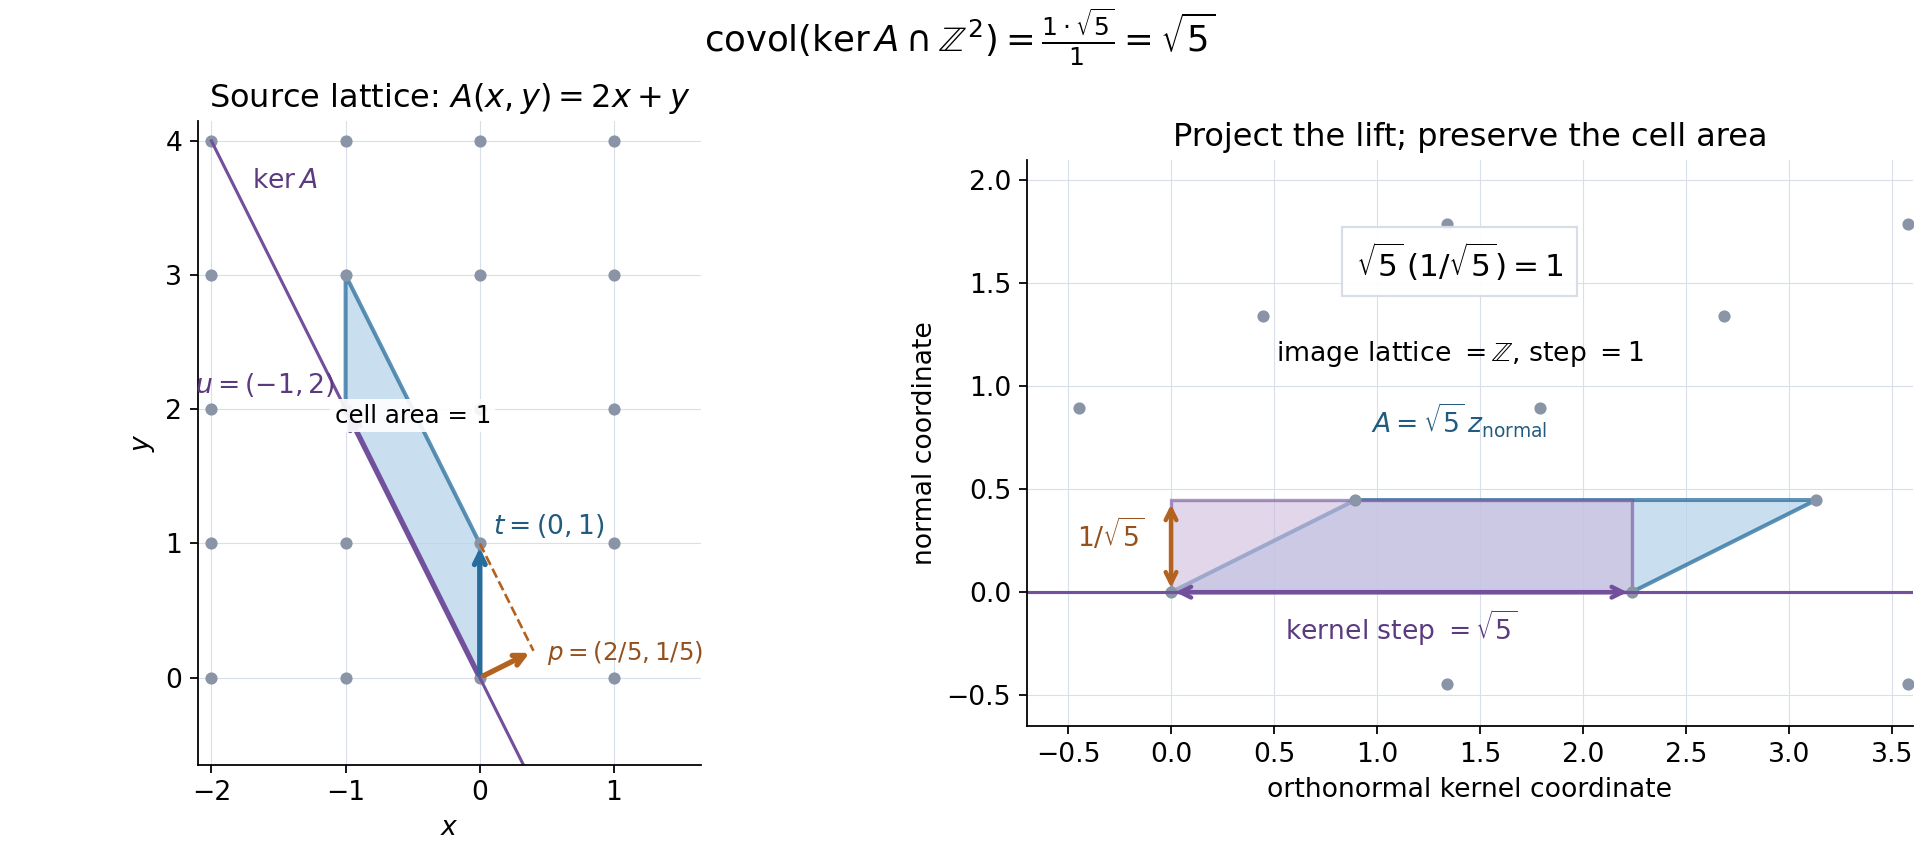
\includegraphics[keepaspectratio,alt={The lattice Z squared, the kernel of A(x,y)=2x+y, an image lift and its orthogonal projection, with the kernel and normal lengths in orthonormal coordinates}]{../figures/kernel-image-volume.png}}
\par\smallskip
\begin{flushleft}\small
\emph{Figure 8.3. For \(A(x,y)=2x+y\) and \(\Gamma=\mathbb Z^2\), the
kernel basis is \(u=(-1,2)\), and \(t=(0,1)\) lifts the image basis
\(1\). The cell with edges \(u,t\) has area \(1\). The orthogonal
projection of \(t\) onto the normal direction is \(p=(2/5,1/5)\), of
length \(1/\sqrt5\). In the right panel the inclined cell and the
rectangle with edges \(u,p\) both have area \(1\); \(p\) is a projected
vector, not a lattice basis vector. The map multiplies normal lengths by
its Jacobian \(\sqrt5\), so (8.43) gives kernel covolume
\(1\cdot\sqrt5/1=\sqrt5\). Reproducible source:
\href{../figure_sources/kernel_image_volume.py}{kernel\_image\_volume.py}.}
\end{flushleft}
\end{minipage}\par\medskip


For a number-field check with finite weights, take
\(K=\mathbb Q(\sqrt2)\), \(\Delta_K=8\),
\(\Gamma=2\mathcal O_K\oplus\mathcal O_K\oplus\mathcal O_K\), and
\(A=(1,\sqrt2,1+\sqrt2)\). Since \(1+\sqrt2\) is a unit,
\(A\Gamma=\mathcal O_K\). The vector \(p=(0,1,-2+\sqrt2)\) lies in the
kernel. With archimedean weights \((2,1/2,1)\) and \((3,5,1)\) at the
two embeddings, and finite weight \(1/4\) in the first column at
\((\sqrt2)\),
\href{../verification/weighted_siegel.py}{weighted\_siegel.py} verifies
(8.43) by exact algebraic Gram determinants and checks (8.45) for this
vector by outward rational intervals. This example checks the metric and
fractional-ideal conventions used in the full proof.

\subsubsection{Weighted integer
relations}\label{weighted-integer-relations}

Several relations require control of a product of vector lengths. We
first establish the geometric theorem that turns a lattice volume into
such a product. This theorem concerns independent lattice vectors;
forming an integer basis is a further step.

\textbf{Theorem (successive minima).} Let \(\Lambda\) be a lattice of
rank \(s\ge1\) in its Euclidean span, and let \(K=-K\) be a compact
convex body with nonempty interior in that span. Define
\(\lambda_i=\lambda_i(K,\Lambda)\) to be the least positive number for
which \(\lambda_iK\) contains \(i\) independent lattice vectors. There
are independent \(a_i\in\lambda_iK\). If their integer span has index
\(J\) in \(\Lambda\), then \[
\frac{2^s}{s!}J\operatorname{covol}(\Lambda)
\le \operatorname{vol}_s(K)\prod_{i=1}^s\lambda_i
\le 2^s\operatorname{covol}(\Lambda).
\tag{8.46}
\] In particular \(J\le s!\). The usual lower bound follows by
\(J\ge1\).

\textbf{Proof.} Discreteness and boundedness make the minima positive
and attained. Choose the vectors in increasing order of their gauges,
keeping a vector whenever it increases the span. This constructs the
\(a_i\) and the flag \[
F_i=\operatorname{span}_{\mathbb R}(a_1,\ldots,a_i),\qquad F_0=0.
\] Every lattice vector in \(\operatorname{int}(\lambda_iK)\) belongs to
\(F_{i-1}\). To check this even when minima coincide, let \(j\) be the
first index of the block with value \(\lambda_i\). The first \(j-1\)
vectors have smaller gauge and span all the lattice vectors of gauge
smaller than \(\lambda_i\). A vector outside that span would make
\(\lambda_j<\lambda_i\), a contradiction.

The convex hull of the \(2s\) points \(\pm a_i/\lambda_i\) lies in
\(K\). Partition it according to the signs of its coordinates in this
basis. Each part is a simplex of volume
\(|\det(a_1,\ldots,a_s)|/(s!\prod_i\lambda_i)\). Their interiors are
disjoint, so this crosspolytope has volume \[
\frac{2^sJ\operatorname{covol}(\Lambda)}
{s!\prod_i\lambda_i}.
\] This proves the lower bound.

Here is a volume proof of the upper bound. An invertible linear change
of variables reduces to \(\Lambda=\mathbb Z^s\). We may also arrange
\(F_i=\operatorname{span}(e_1,\ldots,e_i)\) by a unimodular change of
coordinates. Indeed \(\Lambda\cap F_i\) is primitive: if \(kx\in F_i\),
then \(x\in F_i\). At the first step a primitive generator extends to a
basis by the Euclidean algorithm. In the quotient by that generator the
remaining flag is again primitive. Induction supplies a basis adapted to
the whole flag. These changes preserve volumes because their determinant
has absolute value one.

Put \(Q_i=\lambda_iK/2\), and, for \(N\ge1\), put \[
P_N=\{-N,\ldots,N\}^s,\qquad
P_{N,i}=P_N\cap F_i,\qquad
V_i(N)=\operatorname{vol}_s(P_N+Q_i).
\] The sum denotes a union of translates, not a sum with a convex hull.
Distinct translates of \(Q_1\) have disjoint interiors: an interior
intersection would give a nonzero integer vector in
\(\operatorname{int}(\lambda_1K)\). Thus \[
V_1(N)=(2N+1)^s(\lambda_1/2)^s\operatorname{vol}_s(K).
\] Boundaries have zero volume. For example
\((1-\varepsilon)K\subset\operatorname{int}K\), so their volume is
bounded by
\(\operatorname{vol}(K)-\operatorname{vol}((1-\varepsilon)K)\), which
tends to zero. This also applies to the finite unions here.

We claim, for \(1\le i<s\), \[
V_{i+1}(N)\ge
\left(\frac{\lambda_{i+1}}{\lambda_i}\right)^{s-i}V_i(N).
\tag{8.47}
\] There is nothing to prove if the two minima are equal. Otherwise
write \(t=\lambda_{i+1}/\lambda_i>1\). Two translates of \(Q_{i+1}\)
whose integer centers differ outside \(F_i\) have disjoint interiors. An
intersection would put their difference in
\(\operatorname{int}(\lambda_{i+1}K)\), whereas all lattice vectors
there belong to \(F_i\). Hence, grouping translates by their last
\(s-i\) coordinates, \[
V_j(N)=(2N+1)^{s-i}
\operatorname{vol}_s(P_{N,i}+Q_j)\qquad(j=i,i+1).
\]

Let \(S_t\) multiply coordinates in \(F_i\) by \(t\), leaving the other
coordinates fixed. Its complementary stretch multiplies the last \(s-i\)
coordinates by \(t\) and leaves \(F_i\) fixed. Their product is
multiplication by \(t\), so \[
\operatorname{vol}_s(P_{N,i}+Q_{i+1})
=t^{s-i}\operatorname{vol}_s(P_{N,i}+S_tQ_i).
\] The remaining comparison is \[
\operatorname{vol}_s(A+S_tQ)\ge\operatorname{vol}_s(A+Q)
\quad\text{for every finite }A\subset F_i
\text{ and convex body }Q.
\tag{8.48}
\] Slice at a fixed coordinate \(y\in F_i^\perp\). Write the section of
\(Q\) as \(y+C\), with \(C\subset F_i\) convex. If it is empty the
comparison is immediate. Otherwise choose \(c\in C\). Convexity gives
\(C\subset tC+(1-t)c\), since \(c+(x-c)/t\in C\) for every \(x\in C\).
Consequently \(A+C\subset A+tC+(1-t)c\). The last translation preserves
the section's volume. This proves the inequality section by section;
integration proves (8.48), and hence (8.47).

Iterating (8.47) now gives \[
V_s(N)\ge
(2N+1)^s\frac{\operatorname{vol}_s(K)}{2^s}
\lambda_1^s\prod_{i=1}^{s-1}
\left(\frac{\lambda_{i+1}}{\lambda_i}\right)^{s-i}
=(2N+1)^s\frac{\operatorname{vol}_s(K)}{2^s}
\prod_i\lambda_i.
\] Choose \(R\) so that \(Q_s\subset[-R,R]^s\). Then
\(V_s(N)\le(2N+2R)^s\). Divide by \((2N+1)^s\) and let \(N\) tend to
infinity. This proves the upper bound for \(\mathbb Z^s\); reversing the
first linear change restores \(\operatorname{covol}(\Lambda)\).
\(\square\)

The volume mechanism is Minkowski's; a freely readable treatment is
{[}Henk 2002{]}. The proof above includes the flag construction, the
convex-section inclusion and the boundary and limiting arguments.

\begin{minipage}[t]{\linewidth}
\centering
\pandocbounded{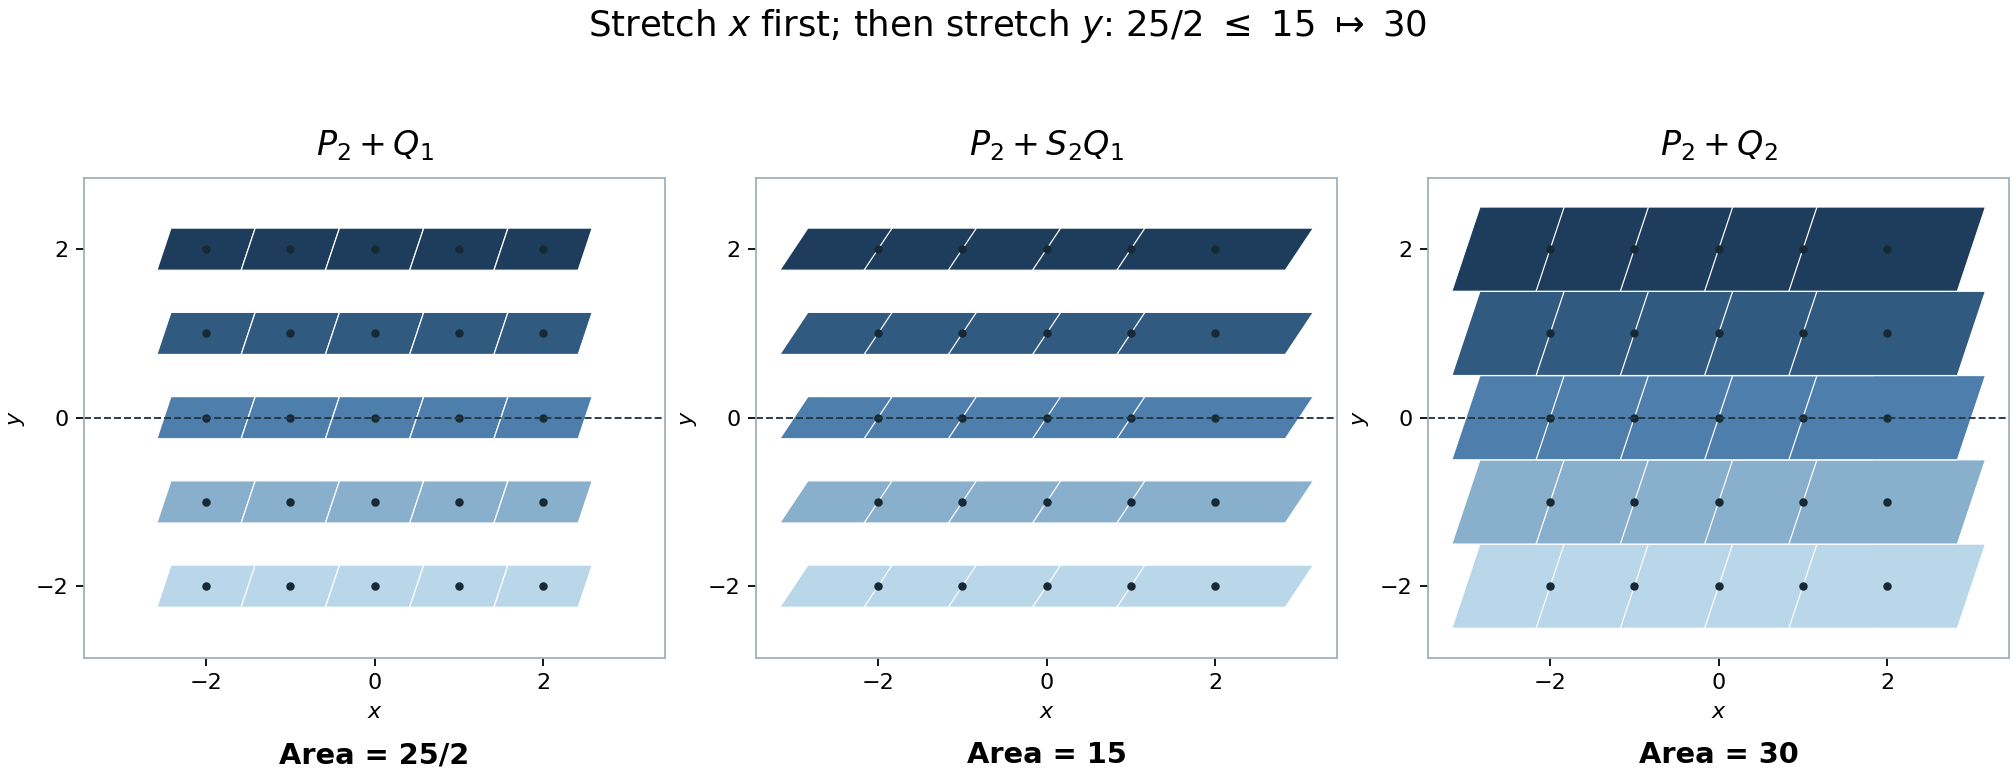
\includegraphics[keepaspectratio,alt={The two stretches in the successive-minimum proof}]{../figures/successive_minima.png}}
\par\smallskip
\begin{flushleft}\small
\emph{The lattice is \(\mathbb Z^2\), and
\(K=\{(x,y):|x-y/3|\le1,\ |y|\le1/2\}\). Its minima are
\(\lambda_1=1,\lambda_2=2\). For \(P_2=\{-2,\ldots,2\}^2\), the three
unions have areas \(25/2,15,30\). Stretching the first coordinate
enlarges every horizontal union of sections; stretching the second
coordinate then doubles area. The resulting inequality is
\(30\ge2(25/2)\), as in (8.47). The limiting bound is exact:
\(\lambda_1\lambda_2\operatorname{area}(K)=4\). Reproducible source:
\href{../figures/successive_minima.py}{successive\_minima.py}.}
\end{flushleft}
\end{minipage}\par\medskip


\textbf{Corollary (an integer basis).} In the same setting, when \(K\)
is the unit ball of a norm, \(\Lambda\) has an integer basis
\(b_1,\ldots,b_s\) such that \[
\|b_i\|\le\max\{1,i/2\}\lambda_i,\qquad
\operatorname{vol}_s(K)\prod_i\|b_i\|
\le2s!\operatorname{covol}(\Lambda).
\tag{8.49}
\]

\textbf{Proof.} Use the flag in the preceding proof. Suppose
\(b_1,\ldots,b_{i-1}\) form a basis of \(\Lambda\cap F_{i-1}\). The
quotient \((\Lambda\cap F_i)/(\Lambda\cap F_{i-1})\) is infinite cyclic.
If \(a_i\) generates it, choose \(b_i=a_i\). Otherwise \(a_i\) is \(m\)
times a generator, with \(m\ge2\). Choose a representative \(b_i\) of
that generator. Its coefficient along \(a_i\) is \(1/m\). By subtracting
integer multiples of the \(a_j\), \(j<i\), make each of its other
coefficients belong to \([-1/2,1/2]\). It still generates the same
quotient and \[
\|b_i\|\le\lambda_i/m+\tfrac12\sum_{j<i}\lambda_j
\le(i/2)\lambda_i.
\] Induction constructs the basis. Finally
\(\prod_{i=1}^s\max\{1,i/2\}=s!/2^{s-1}\); combine this with (8.46). For
\(s=1\) the constant is exactly two, the length of the unit interval.
\(\square\)

For later comparison it is useful to spell out what follows with
Euclidean geometry alone.

\textbf{Lemma (Euclidean product bound for weighted relations).} Let
\(v_1,\ldots,v_n\) generate a rank-\(r\) lattice \(M\), where
\(1\le r<n\), in a normed real space. Choose \(A_j>0\) with
\(\|v_j\|\le A_j\), and let \(B_r\) have the meaning in (8.31). There
are \(s=n-r\) independent integer relations \(\sum_j u_{ij}v_j=0\) with
\[
\prod_{i=1}^{s}\max_j A_j|u_{ij}|
\le
\frac{2^s\Gamma(1+s/2)}{\pi^{s/2}}
\binom nr^{1/2}
\frac{B_r}{\operatorname{covol}_r(M)}
\prod_{j=1}^n A_j.
\tag{8.50}
\] The relations are independent; they need not form a basis of all the
integer relations.

\textbf{Proof.} In an integer basis of \(M\), write the vectors as the
columns of a surjective integer matrix \(C:\mathbb Z^n\to\mathbb Z^r\).
Give \(\mathbb R^n\) the metric \(\|x\|_{A,2}^2=\sum_j A_j^2x_j^2\). The
kernel-volume identity (8.43), in its rational-field case, gives \[
\operatorname{covol}_{A,2}(\ker C\cap\mathbb Z^n)
=\left(\prod_j A_j\right)
\sqrt{\det(C\operatorname{diag}(A_j^{-2})C^{\mathsf t})}.
\] There is no image-index factor: \(C\mathbb Z^n=\mathbb Z^r\). By
Cauchy--Binet the determinant under the square root is \[
\sum_{|I|=r}\frac{\det(C_I)^2}{\prod_{j\in I}A_j^2}.
\] The parallelepiped spanned by the \(v_j\), \(j\in I\), has volume
\(|\det C_I|\operatorname{covol}_r(M)\). After normalizing each edge,
its volume is at most \(B_r\). Every summand is therefore at most
\((B_r/\operatorname{covol}_r(M))^2\). This bounds the kernel covolume
by the last three factors in (8.50).

The Euclidean unit ball in this \(s\)-dimensional kernel has volume
\(\pi^{s/2}/\Gamma(1+s/2)\) in the same metric. Apply the upper bound
(8.46) and choose independent vectors at its successive minima. Since
\(\max_j A_j|u_j|\le\|u\|_{A,2}\), their weighted maximum norms satisfy
(8.50). \(\square\)

The Euclidean ball accounts for the factor
\(2^s\Gamma(1+s/2)/\pi^{s/2}\). A sharper product estimate using a
section of the weighted cube requires a lower bound for that section's
volume. The round-ball argument alone does not supply that sharper
constant.

\subsubsection{Sections of a cube and the sharp product
estimate}\label{sections-of-a-cube-and-the-sharp-product-estimate}

We now supply the missing geometric input. The proof uses nearest points
on faces and a comparison of their Gram matrices.

\textbf{Lemma (face distances and volume).} Let \(P\subset\mathbb R^s\)
be a full-dimensional convex polyhedron with \(0\) in its interior.
Suppose that, for every nonempty face \(F\) of codimension \(i\),
\(\operatorname{dist}(0,\operatorname{aff}F)\ge\sqrt i\). Then \[
\operatorname{vol}_s(P)\ge2^s.
\tag{8.51}
\]

\textbf{Proof.} If \(P\) is unbounded, its volume is infinite. Indeed,
write its finitely many defining inequalities as \(g_j(x)\le d_j\).
Normalize an unbounded sequence of points and take a convergent
subsequence of their directions. Its unit limit \(w\) has \(g_j(w)\le0\)
for every \(j\). Thus \(P+[0,\infty)w\subset P\). Translating a small
ball about zero along this ray supplies a cylinder of infinite volume.
We may therefore assume that \(P\) is a polytope.

For every face \(F\), choose its point \(a_F\) closest to zero.
Existence follows from compactness, and uniqueness from strict convexity
of squared Euclidean length. If \(y\in F\), differentiation at zero
along \(a_F+t(y-a_F)\) gives \[
a_F\cdot y\ge |a_F|^2.
\] Choose a full flag \(P=F_0\supset F_1\supset\cdots\supset F_s\),
where \(F_i\) has codimension \(i\), and put \(a_i=a_{F_i}\). Here
\(a_0=0\). Since \(a_j\in F_i\) when \(j\ge i\), \[
a_i\cdot a_j\ge |a_i|^2\ge i
\quad(1\le i\le j\le s).
\tag{8.52}
\] The final inequality uses the distance to the affine span. It does
not require the nearest point of that affine span to belong to the face.

The simplices \(A=\operatorname{conv}(a_0,\ldots,a_s)\) over all full
flags cover \(P\), with disjoint interiors for the nondegenerate
simplices. To see this, triangulate each face recursively by coning its
already triangulated facets to \(a_F\). Coning still works if \(a_F\)
lies on its boundary. For a relative interior point other than \(a_F\),
its ray from \(a_F\) meets a far boundary facet. That facet is unique
except on rays meeting the lower-dimensional face intersections. Those
exceptional cones have zero volume; facets containing \(a_F\) likewise
contribute only degenerate cones. Induction on the face dimension gives
exactly the flag simplices and proves the asserted partition for volume
calculations.

For a nondegenerate \(A\), let \(f\) be the linear map taking \(a_i\) to
\[
c_i=(\underbrace{1,\ldots,1}_{i},0,\ldots,0),\qquad c_0=0.
\] These target vectors form a basis, so \(f\) is invertible. For
\(x=\sum_{i=1}^s t_i a_i\in A\), the barycentric coefficients satisfy
\(t_i\ge0\) and \(\sum_i t_i\le1\). Because \(c_i\cdot c_j=\min(i,j)\),
(8.52) yields directly \[
|x|^2
=\sum_{i,j}t_it_j(a_i\cdot a_j)
\ge\sum_{i,j}t_it_j\min(i,j)
=|f(x)|^2.
\] This is a comparison on the simplex, where the coefficients are
nonnegative; it does not claim that \(f\) contracts every vector in the
ambient space.

Write \(C=\operatorname{conv}(c_0,\ldots,c_s)\), and let \(\mathbb B_s\)
be the Euclidean unit ball. The last inequality gives
\(f(A\cap\mathbb B_s)\subset C\cap\mathbb B_s\). An invertible linear
map scales every volume by the same determinant, so \[
\frac{\operatorname{vol}(A\cap\mathbb B_s)}{\operatorname{vol}(A)}
\le
\frac{\operatorname{vol}(C\cap\mathbb B_s)}{\operatorname{vol}(C)}
=\frac{\operatorname{vol}(\mathbb B_s)}{2^s}.
\] For the last equality, partition \([-1,1]^s\) by coordinate signs and
the orders of their absolute values. Its \(2^ss!\) pieces are congruent
to \(C=\{1\ge x_1\ge\cdots\ge x_s\ge0\}\). The orthogonal sign and
permutation maps preserve \(\mathbb B_s\). Each piece therefore has the
same fraction of the ball and the same volume, proving the equality.

The face-distance hypothesis for facets makes \(\mathbb B_s\subset P\):
every defining supporting halfspace contains that ball. Sum the
preceding inequality over the nondegenerate flag simplices. Their
intersections partition the ball up to zero-volume sets, giving \[
\operatorname{vol}(\mathbb B_s)
\le\frac{\operatorname{vol}(\mathbb B_s)}{2^s}
\operatorname{vol}(P).
\] Cancel the positive ball volume to prove (8.51). \(\square\)

This is the nearest-face volume mechanism of Rogers, as presented in
{[}Karasev 2026{]}. The Gram comparison (8.52) supplies a direct map
from each nondegenerate flag simplex to \(C\).

\textbf{Theorem (central sections of a cube).} For every
\(s\)-dimensional linear subspace \(E\subset\mathbb R^n\), \[
\operatorname{vol}_s(E\cap[-1,1]^n)\ge2^s.
\tag{8.53}
\] The volume uses the induced Euclidean metric on \(E\).

\textbf{Proof.} The section is a full-dimensional polytope in \(E\) and
contains its unit ball. A codimension-\(i\) face is obtained by active
coordinate constraints \(x_j=1\) or \(x_j=-1\), whose restrictions to
\(E\) have rank \(i\). This rank assertion can be checked at a relative
interior point of the face: the inactive inequalities remain strict in a
neighborhood, so its tangent space is exactly the simultaneous kernel of
the active coordinate forms. Select \(i\) independent active forms, with
distinct indices. Every point of the affine span of that face has those
\(i\) coordinates of modulus one, and consequently has squared Euclidean
length at least \(i\). Apply (8.51) in \(E\). For \(s=0\), the
corresponding zero-dimensional statement is \(1\ge1\). \(\square\)

The result is Vaaler's cube-section theorem. The proof above establishes
it in all dimensions; it uses neither a hyperplane-only estimate nor an
assumption on rational directions.

\begin{minipage}[t]{\linewidth}
\centering
\pandocbounded{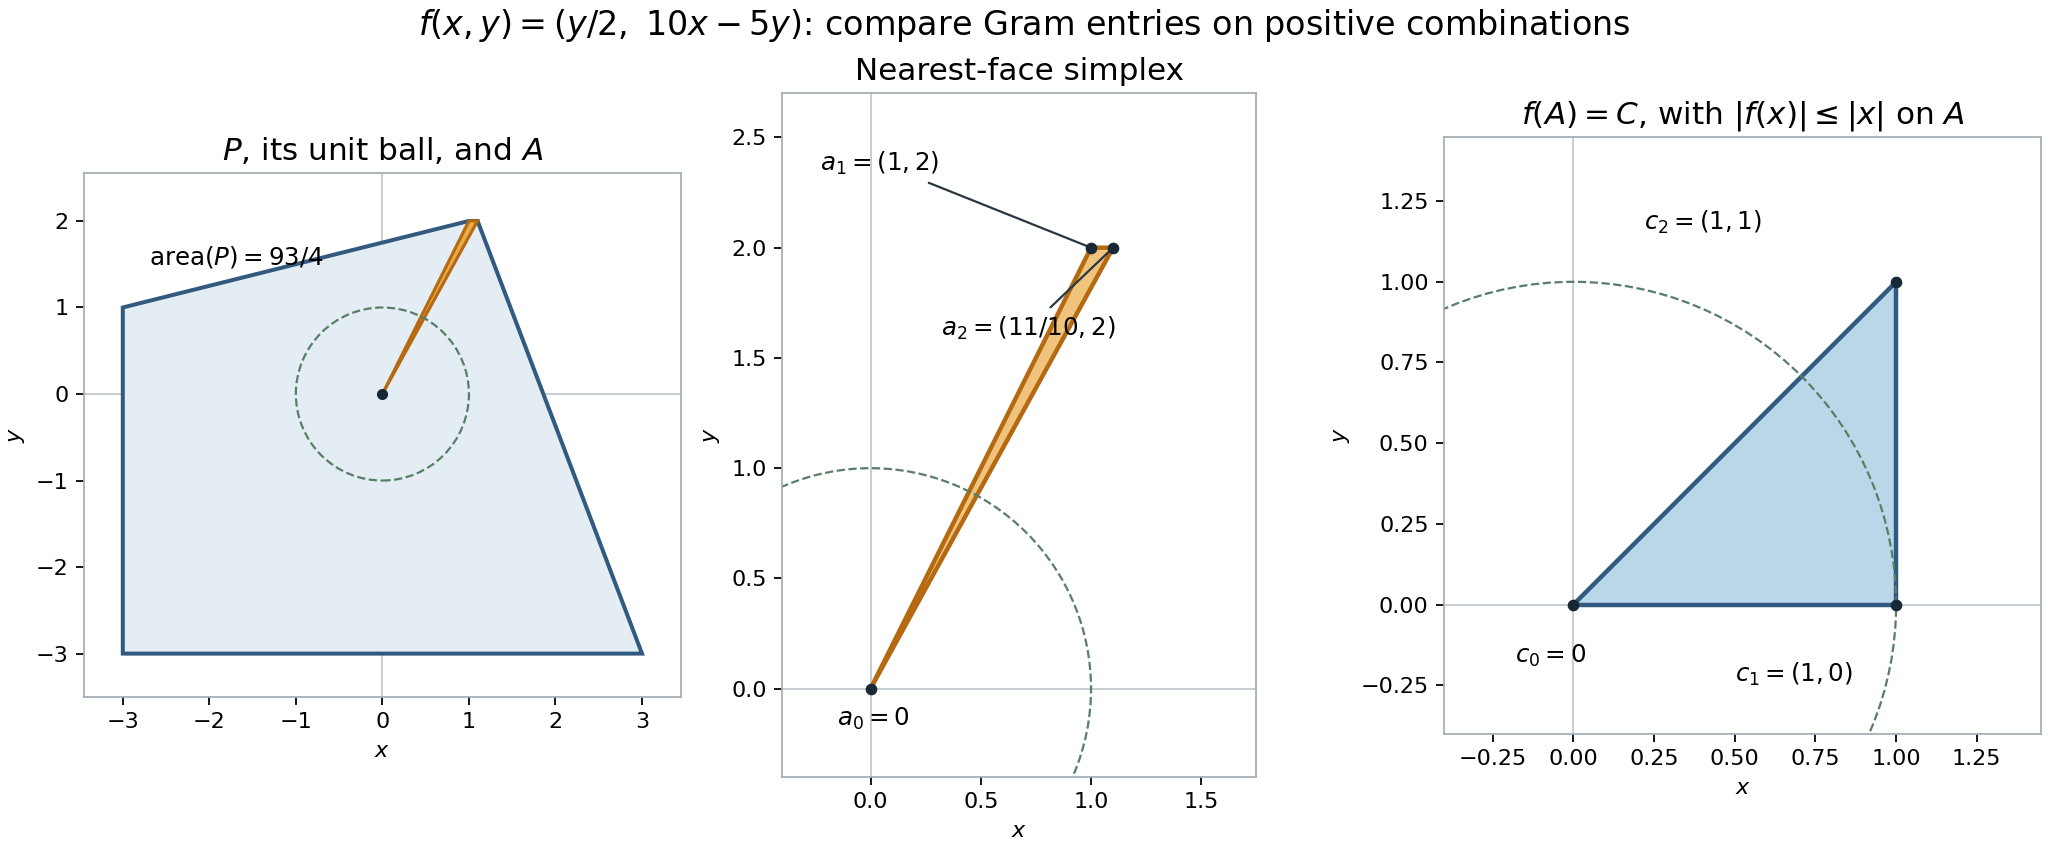
\includegraphics[keepaspectratio,alt={The Gram comparison for a nearest-face simplex}]{../figures/face_gram.png}}
\par\smallskip
\begin{flushleft}\small
\emph{The polytope has vertices
\((1,2),(11/10,2),(3,-3),(-3,-3),(-3,1)\). The highlighted flag simplex
is \(A=\operatorname{conv}\{0,(1,2),(11/10,2)\}\). Its nearest point on
the top edge is the endpoint \((1,2)\). The comparison map
\(f(x,y)=(y/2,10x-5y)\) takes \(A\) to
\(C=\operatorname{conv}\{0,(1,0),(1,1)\}\). The difference of the two
vertex Gram matrices is
\(\left(\begin{smallmatrix}4&41/10\\41/10&321/100\end{smallmatrix}\right)\),
whose entries are positive. Thus \(|f(x)|\le|x|\) on \(A\), by
nonnegative barycentric coefficients in (8.52). The same map expands the
ambient vector \((1/10,0)\) to \((0,1)\); a contraction on the simplex
does not imply a contraction everywhere. Reproducible source:
\href{../figures/face_gram.py}{face\_gram.py}.}
\end{flushleft}
\end{minipage}\par\medskip


\textbf{Corollary (sharp product bound for weighted relations).} Under
the hypotheses of (8.50), there are \(s=n-r\) independent integer
relations satisfying \[
\prod_{i=1}^{s}\max_j A_j|u_{ij}|
\le
\binom nr^{1/2}
\frac{B_r}{\operatorname{covol}_r(M)}
\prod_{j=1}^n A_j.
\tag{8.54}
\]

\textbf{Proof.} Use the same relation lattice and weighted Euclidean
covolume calculation as in (8.50). The map
\(x\mapsto(A_1x_1,\ldots,A_nx_n)\) is an isometry for that metric. It
takes the weighted maximum-norm unit ball in the real kernel to a
central section of \([-1,1]^n\). Its \(s\)-volume is therefore at least
\(2^s\), by (8.53). Minkowski's upper product estimate (8.46) bounds the
product of its successive minima by the kernel covolume. Choose
independent integer vectors at these minima and use the covolume bound
already proved in (8.50). This gives (8.54). \(\square\)

This supplies the full weighted relation estimate of {[}Matveev 2000{]},
with the binomial square root and with no basis assertion. In dimension
one, the maximal-minor argument below removes that square root as well.

For a one-dimensional relation space the following stronger estimate
removes the binomial square root. It applies to real lattice vectors and
does not require their coordinates to be rational.

\textbf{Lemma (a relation of codimension one).} Let \(v_1,\ldots,v_n\)
generate an \((n-1)\)-dimensional lattice \(M\) in a normed real space.
Suppose \(0<\|v_j\|\le A_j\). Let \(B_{n-1}\) be the supremum of the
Euclidean volumes of parallelepipeds with \(n-1\) edges of norm at most
one. There is a primitive nonzero \(u\in\mathbb Z^n\), unique up to
sign, with \(\sum_j u_jv_j=0\), and \[
|u_j|A_j\le
\frac{B_{n-1}}{\operatorname{covol}_{n-1}(M)}
\prod_{k=1}^n A_k
\qquad(1\le j\le n).
\tag{8.55}
\]

\textbf{Proof.} In an integer basis of \(M\), the columns \(v_j\) form
an integer matrix \(C\) of size \((n-1)\times n\), whose map
\(\mathbb Z^n\to\mathbb Z^{n-1}\) is surjective. Its real kernel is a
rational line. The integer points on that line are \(\mathbb Z u\) for
one primitive integer vector \(u\): divide any nonzero integer generator
by the greatest common divisor of its coordinates.

A primitive integer vector extends to an integer basis of
\(\mathbb Z^n\). Here is the elementary argument. The Euclidean
algorithm on a pair of coordinates is effected by swaps, sign changes
and adding an integer multiple of one row to another. Apply it
repeatedly to replace the coordinates of \(u\) by their greatest common
divisor and zeros. Primitivity makes the nonzero coordinate one. The
resulting integer matrix has determinant \(\pm1\); its inverse gives the
asserted basis. Let \(U\) be its matrix with first column \(u\). Then
\(CU=(0,C')\), and \(C'\) is a square surjective integer matrix.
Surjectivity supplies an integer right inverse, so \(\det C'=\pm1\).

For every real row \(f\), multiply the square matrix with first row
\(f\) and remaining rows \(C\) by \(U\). Expanding on its first column
gives \[
\det\begin{pmatrix}f\\C\end{pmatrix}
=\pm f\cdot u.
\] Expanding the original matrix on its first row shows that each signed
maximal minor of \(C\) is the corresponding coordinate of \(\pm u\).
Therefore the parallelepiped spanned by all \(v_k\) except \(v_j\) has
volume exactly \(|u_j|\operatorname{covol}_{n-1}(M)\). After dividing
its edges by their \(A_k\), the defining bound for \(B_{n-1}\) gives \[
|u_j|\operatorname{covol}_{n-1}(M)
\le B_{n-1}\prod_{k\ne j}A_k.
\] Multiply by \(A_j\) to obtain (8.55). \(\square\)

In the logarithmic coordinate space use \(\mathcal H\) as the norm.
Equations (8.28)--(8.31) then give explicit numerical coefficients in
(8.55). The continuous unit ball in the definition of \(B_r\) matters:
normalized edges \(v_j/A_j\) are real vectors and need not themselves be
logarithms of algebraic numbers.

The coefficient parameter survives a reduction in the number of
logarithms only if the integer relation is bounded with the same
weights. Here is the precise linear algebra needed for that reduction.

\textbf{Lemma (weighted minors).} Let \(H_j>0\), with
\(H_1\le\cdots\le H_{n-1}\), and define \[
\|x\|_H=\sum_jH_j|x_j|,\qquad
|x|_H=\max_jH_j|x_j|.
\] Let \(x_1,\ldots,x_\nu\in\mathbb Z^n\) be linearly independent,
\(1\le\nu\le n\), and let \(b\in\mathbb Z^n\), \(b_n\ne0\), belong to
their rational span. If \(\|x_i\|_H\le X_i\), there are integers
\(m_0,\ldots,m_\nu\), with \(m_0\ne0\), such that \[
m_0b=\sum_{i=1}^\nu m_ix_i,\qquad
|m_0|\le Q,\quad |m_i|X_i\le\nu|b|_H Q,
\] where \[
Q=\frac{\prod_{i=1}^\nu X_i}{H_1\cdots H_{\nu-1}H_n}.
\] With the assumptions \(|x_i|_H\le X_i\) instead, the bounds are \[
|m_0|\le\nu^{\nu/2}Q,\qquad
|m_i|X_i\le\nu^{\nu/2}|b|_H Q.
\]

\textbf{Proof.} Since \(b_n\ne0\), column \(n\) of the matrix with rows
\(x_i\) is nonzero. Extend this column to a set \(J\) of \(\nu\)
independent columns. Its determinant \(\Delta\) is a nonzero integer.
Cramer's rule gives the unique coefficients in the selected coordinates
as \(\Delta_i/\Delta\), where \(\Delta_i\) replaces row \(i\) by the
selected coordinates of \(b\). They give the relation in every
coordinate, because \(b\) lies in the full row span and the selected
minor detects its unique coordinates there. Take \(m_0=\Delta\),
\(m_i=\Delta_i\).

Multiply selected column \(j\) by \(H_j\), and divide row \(i\) by
\(X_i\). Each resulting row has sum of absolute values at most one, so
its determinant has modulus at most one: its Leibniz sum is bounded by
the product of these row sums. For the replaced row, divide instead by
\(\nu|b|_H\). The same argument applies, and \[
\prod_{j\in J}H_j\ge H_1\cdots H_{\nu-1}H_n.
\] These observations prove the first pair of bounds. Under the max-norm
hypotheses, normalized rows have Euclidean norm at most \(\sqrt\nu\),
and the normalized replacement row has the same bound after division by
\(|b|_H\). Hadamard's inequality gives the factor \(\nu^{\nu/2}\) in
both bounds. \(\square\)

This proves the weighted reduction lemma used in {[}Matveev 2000{]},
without requiring the selected vectors to form a basis of their ambient
integer lattice.

The two modern estimates use the same group-theoretic zero mechanism. We
establish it now, before applying it to the auxiliary function and later
to the derivative determinant. The weighted relation lemmas above supply
its arithmetic constants.

\subsubsection{Algebraic groups and transverse
jets}\label{algebraic-groups-and-transverse-jets}

The rank argument takes place in a product of additive and
multiplicative groups. We first establish the group and derivative facts
that make its multiplicity factor explicit. Throughout this subsection,
\(k\) is an algebraically closed field of characteristic zero, and \[
G=k^{d_0}\times(k^\times)^{d_1},\qquad
R=k[X_1,\ldots,X_{d_0},Y_1^{\pm1},\ldots,Y_{d_1}^{\pm1}].
\] Write the group law additively, even in the multiplicative
coordinates: translation by \(g=(x,y)\) substitutes \(X+x\) and \(yY\).
For \(w=(\xi,\eta)\in k^{d_0+d_1}\), put \[
D_w=\sum_i\xi_i\partial_{X_i}+
\sum_j\eta_jY_j\partial_{Y_j}.
\tag{8.56}
\] These derivations commute with one another and with translations.
Indeed, the coordinate operators in different variables commute, and the
two assertions in a single variable follow directly from the additive
substitution \(X_i+x_i\) and the multiplicative substitution \(y_jY_j\).

\textbf{Lemma (subgroups and their tangent directions).} Every closed
algebraic subgroup \(H\) of \(G\) has the form \[
H=V\times T_\Phi,\qquad
T_\Phi=\{y:Y^u=1\text{ for every }u\in\Phi\},
\tag{8.57}
\] where \(V\subseteq k^{d_0}\) is a vector subspace and
\(\Phi\subseteq\mathbb Z^{d_1}\) is a subgroup. Its ideal is generated
by the linear forms vanishing on \(V\) and the elements \(Y^u-1\),
\(u\in\Phi\). If the tangent space is defined by \[
T(H)=\{w:D_wI(H)\subseteq I(H)\},
\] then \[
T(H)=V\times\Phi^\perp,\qquad
\Phi^\perp=\{\eta:u\cdot\eta=0\text{ for every }u\in\Phi\}.
\tag{8.58}
\] The identity component is obtained by replacing \(\Phi\) by its
saturation \(\Phi^{\rm sat}=\mathbb Q\Phi\cap\mathbb Z^{d_1}\); it has
the same tangent space.

\textbf{Proof.} Let \(V\) initially denote the Zariski closure of the
additive projection of \(H\). It is an additive subgroup. To see this
directly, polynomials vanishing on that projection also vanish after
addition of two points of its closure: first hold one projected point
fixed and use density in the other variable, then use density in the
fixed variable. Inversion is handled in the same way. For \(v\in V\),
the points \(mv\), \(m\in\mathbb Z\), lie in \(V\). Every polynomial
defining \(V\), evaluated on \(tv\), is a polynomial in \(t\) with
infinitely many zeros. Characteristic zero makes those integer values
distinct, so \(kv\subseteq V\). Closure under sums now shows that \(V\)
is a vector subspace.

Define \(\Phi=\{u:Y^u|_H=1\}\). Two monomial characters have the same
restriction to \(H\) precisely when their exponent difference lies in
\(\Phi\). Modulo the indicated character relations, a Laurent polynomial
can therefore be written as a finite sum \[
\sum_a Y^a p_a(X)
\] with pairwise distinct characters \(Y^a|_H\). We show that this sum
vanishes on \(H\) only if every \(p_a\) vanishes on its additive
projection.

Let \(h\) bound the degrees of the \(p_a\), and write \(T_g\) for
translation on polynomial functions. On the block \(Y^a p(X)\), \(T_g\)
is its character value \(y^a\) times translation by \(x\) on polynomials
of degree at most \(h\). Thus \(T_g-y^a\) is nilpotent of order at most
\(h+1\) on this block: each finite difference lowers polynomial degree.
Fix a block \(a\). For every other block \(b\), choose \(g_b\in H\) such
that \(y_b^a\ne y_b^b\), and apply \[
\prod_{b\ne a}(T_{g_b}-y_b^b)^{h+1}.
\] The factors commute. They annihilate every other block and are
invertible on block \(a\): there each factor is a nonzero scalar plus a
nilpotent operator, whose inverse is a finite geometric sum. These
operators and their inverses preserve the property of vanishing on
\(H\), since they are linear combinations of translations by its
elements. Hence \(Y^a p_a(X)\), and therefore \(p_a(X)\), vanishes on
\(H\). It follows that \(p_a\) vanishes on \(V\).

After a linear coordinate change, \(I(V)\) is generated by coordinate
variables: a polynomial zero on the remaining coordinate space has zero
constant term in those variables. This proves the asserted description
of \(I(H)\). Taking its zero set gives (8.57). Moreover, a finite basis
of \(\Phi\) suffices for its character relations, because \[
Y^{u+v}-1=Y^u(Y^v-1)+(Y^u-1),\qquad
Y^{-u}-1=-Y^{-u}(Y^u-1).
\]

For a linear form \(L\) vanishing on \(V\), \(D_wL=L(\xi)\). For
\(u\in\Phi\), \[
D_w(Y^u-1)=(u\cdot\eta)Y^u
\equiv u\cdot\eta\pmod{I(H)}.
\] The derivation preserves the ideal generated by these functions
exactly under the conditions in (8.58).

The lattice argument in Section 4 gives a finite integer basis of
\(\Phi\), since it is a discrete subgroup of \(\mathbb R^{d_1}\). For
completeness, integer row and column operations put a basis matrix of
\(\Phi\) into diagonal form. The reduction uses the Euclidean algorithm:
move a nonzero entry to the first position and reduce other entries in
its row and column by division. If the resulting pivot does not divide
some remaining entry, add that entry's row to the pivot row and divide
again; the positive pivot strictly decreases. Eventually it divides all
remaining entries. Clear its row and column and repeat on the remaining
matrix. All operations are invertible over \(\mathbb Z\), and the
process ends because each pivot reduction strictly decreases a positive
integer. The resulting torus coordinate change is a monomial
automorphism. In the new coordinates the relations are \(Y_i^{c_i}=1\),
\(1\le i\le r\), where \(r=\operatorname{rank}\Phi\). Each \(c_i\)-th
root is a distinct point in characteristic zero, and each choice leaves
a torus of dimension \(d_1-r\). Together with \(V\), these are disjoint
irreducible components: their coordinate rings are polynomial Laurent
domains. The component through the identity sets these first \(r\)
coordinates equal to one, which is exactly the saturation of \(\Phi\).
Its annihilator over \(k\) equals that of \(\Phi\), proving the last
claim. \(\square\)

Let \(W\subseteq k^{d_0+d_1}\) be a vector subspace, and put
\(\ell=\dim(W/(W\cap T(H)))\). Choose \(w_1,\ldots,w_\ell\in W\)
independent modulo \(T(H)\). The preceding generators of \(I(H)\), and
their derivatives modulo that ideal, give a bilinear pairing with left
kernel \(T(H)\). Linear algebra therefore gives
\(P_1,\ldots,P_\ell\in I(H)\) such that \[
D_{w_i}P_j\equiv\delta_{ij}\pmod{I(H)}.
\] This assertion extends to a finite union \(Z=\bigcup_{a=1}^s(g_a+H)\)
of distinct cosets.

Indeed, whenever \(g\notin H\), one of the displayed generators gives a
function zero on \(H\) and a nonzero constant on \(g+H\). Divide by that
constant to get \(A_g\), equal to one on \(g+H\). Put \[
B_a=\prod_{b\ne a}A_{g_a-g_b}\circ T_{-g_b},
\qquad
Q_j=\sum_{a=1}^s B_a^2(P_j\circ T_{-g_a}).
\] On \(g_a+H\), \(B_a=1\), while every other \(B_b=0\). Thus
\(Q_j\in J:=I(Z)\), and differentiation gives \[
D_{w_i}Q_j\equiv\delta_{ij}\pmod J.
\] The terms differentiating \(B_a^2\) vanish on the same coset because
\(P_j\circ T_{-g_a}=0\) there, and on every other coset because
\(B_a=0\) there.

\textbf{Lemma (transverse jet count).} Give \(R\) its multidegree
filtration \(F_D\): total additive degree is at most \(D_0\), and the
absolute exponent in each \(Y_j\) is at most \(D_j\). For an ideal
\(A\subseteq R\), write \[
\mathcal H_A(D)=\dim_k(F_D/(A\cap F_D)).
\] Suppose every element of \(A\) vanishes on \(Z\), with all
derivatives along \(W\) of total order at most \(S\). Choose a
multidegree bound \(C\) for the \(Q_j\) above. Then, for every \(D\), \[
\mathcal H_A(D+SC)\ge
\binom{S+\ell}{\ell}\mathcal H_J(D).
\tag{8.59}
\] No primarity assumption on \(A\) is needed for this filtered
inequality.

\textbf{Proof.} For multi-indices
\(\alpha,\beta\in\mathbb Z_{\ge0}^{\ell}\) with \(|\beta|\le|\alpha|\),
the Leibniz rule gives \[
D_{w_1}^{\beta_1}\cdots D_{w_\ell}^{\beta_\ell}
\left(PQ_1^{\alpha_1}\cdots Q_\ell^{\alpha_\ell}\right)
\equiv
\begin{cases}
\alpha!P,&\beta=\alpha,\\
0,&\beta\ne\alpha
\end{cases}
\pmod J.
\tag{8.60}
\] When fewer than \(|\alpha|\) derivatives are applied, at least one
undifferentiated \(Q_j\) remains in each Leibniz term. When exactly
\(|\alpha|\) are applied, a term can survive modulo \(J\) only if each
\(Q\)-factor receives exactly one derivative and \(P\) receives none.
The congruences \(D_{w_i}Q_j=\delta_{ij}\) modulo \(J\) then require
\(\beta=\alpha\) and give the factor \(\alpha!\). This proves (8.60).

Choose \(E\subseteq F_D\) complementary to \(F_D\cap J\), with basis
\(P_1,\ldots,P_N\); here \(N=\mathcal H_J(D)\). The products
\(P_iQ^\alpha\), \(1\le i\le N\), \(|\alpha|\le S\), have degree at most
\(D+SC\). They are independent modulo \(A\). Otherwise write a nonzero
relation as \(\sum_\alpha P_\alpha Q^\alpha\in A\), \(P_\alpha\in E\),
and choose a nonzero \(P_\beta\) of minimum total index degree. Apply
\(D^\beta\). The derivative lies in \(J\) by hypothesis, whereas (8.60)
makes it congruent to \(\beta!P_\beta\). Characteristic zero and
\(E\cap J=0\) give a contradiction. There are \(\binom{S+\ell}{\ell}\)
indices, proving (8.59). \(\square\)

This is the linear-algebraic multiplicity factor in Wüstholz's lemma;
compare {[}Waldschmidt 2000{]}. The proof here gives the filtered
inequality directly. To obtain a bound on the leading degree of an
intersection one must also control its dimension and multigraded Hilbert
function.

For a concrete example, let \(G=k\times k^\times\), \(H=\{(0,1)\}\),
\(Q_1=X\), \(Q_2=Y-1\), and let \(W\) have basis
\(\partial_X,Y\partial_Y\). The two first derivatives give the identity
matrix modulo \(J=(X,Y-1)\). For \(S=2\), the six products \[
1,\ X,\ Y-1,\ X^2,\ X(Y-1),\ (Y-1)^2
\] are independent modulo \(J^3\). In fact they form a basis of
\(R/J^3\): terms of degree at least three vanish, and
\(Y^{-1}=(1+(Y-1))^{-1}\equiv1-(Y-1)+(Y-1)^2\). The ordinary derivative
matrix has determinant \(4\); dividing row \(\beta\) by \(\beta!\) gives
determinant one. Thus the multiplicity count \(\binom42=6\) is attained
exactly. \href{../verification/auxiliary_jets.py}{auxiliary\_jets.py}
verifies the matrix and the vanishing of all degree-three generators
under the six jets.

\subsubsection{Hilbert functions and the multiplicity
degree}\label{hilbert-functions-and-the-multiplicity-degree}

We need the leading degree of the filtered functions just introduced.
The Noether normalization theorem proved in
\href{../../AG-CA/krull-dimension-and-noether-normalization.html\#3-normalization-that-respects-ideals}{\emph{Krull
dimension and Noether normalization}}, Corollary 3.2, applies to every
nonzero finite-type \(k\)-algebra, including a nonreduced algebra. It
contains an embedded polynomial algebra over which it is finite. Theorem
4.2 and the paragraph following its proof in
\href{../../AG-CA/krull-dimension-and-noether-normalization.html\#4-parameters-measure-dimension-and-height}{Section
4 of that lesson} show that the number of parameters is its Krull
dimension. We use this full form below.

The following argument supplies the multigraded filtration needed here.

\textbf{Lemma (multigraded polynomial and dimension).} For a proper
ideal \(A\subset R\), \(\mathcal H_A(D)\) agrees with a polynomial
\(p_A(D_0,\ldots,D_{d_1})\) when all coordinates are sufficiently large.
Its total degree is \(e=\dim(R/A)\). Write \(p_{A,e}\) for its
homogeneous part of degree \(e\), and define \[
H(A;D)=e!\,p_{A,e}(D).
\tag{8.61}
\] This polynomial is strictly positive when every coordinate of \(D\)
is positive. A fixed shift of the filtration has the same leading part.
If \(A\subseteq B\) are proper ideals of the same dimension, then
\(H(B;D)\le H(A;D)\) for every \(D\ge0\).

\textbf{Proof.} Introduce a polynomial ring with one additive block
\((t_0,X_1,\ldots,X_{d_0})\), and multiplicative blocks
\((t_j,Y_j,Z_j)\), \(1\le j\le d_1\). A polynomial homogeneous of degree
\(D_i\) in every block maps onto \(F_D\) by setting every \(t_i=1\) and
\(Z_j=Y_j^{-1}\). Surjectivity follows by homogenizing each Laurent
monomial: use \(Y_j^{u_j}\) for \(u_j\ge0\), \(Z_j^{-u_j}\) otherwise,
and pad with \(t_j^{D_j-|u_j|}\); pad the additive monomial in the same
way. Let \(\widetilde A\) be the direct sum, over all multidegrees, of
the kernels of these maps followed by reduction modulo \(A\).
Multiplication respects the evaluation maps, so \(\widetilde A\) is a
multihomogeneous ideal. Its quotient has multidegree-\(D\) dimension
exactly \(\mathcal H_A(D)\).

We give the polynomial count explicitly. Choose a monomial order and let
\(M\) be the ideal generated by the leading monomials of elements of
\(\widetilde A\). This monomial ideal has finitely many minimal
generators. Here is the finite combinatorial fact needed for that
assertion: every infinite sequence in \(\mathbb Z_{\ge0}^q\) has an
infinite subsequence nondecreasing in every coordinate. For one
coordinate, either some value occurs infinitely often or one can
successively choose increasing values. Repeat for the finitely many
coordinates. Thus an infinite set of incomparable minimal exponent
vectors is impossible. Every exponent vector above a minimal one is a
multiple of it, which proves finite generation of \(M\).

Choose a multihomogeneous polynomial for each of those leading
monomials. Polynomial division by this finite list shows that the
monomials outside \(M\) span the quotient, with multidegree preserved.
They are independent: a nonzero linear combination in \(\widetilde A\)
would have a leading monomial in \(M\). Hence they are a basis in each
multidegree. If a block contains \(q_i\) variables, the number of its
monomials of degree \(D_i\) divisible by a fixed monomial of block
degree \(c_i\) is \[
\binom{D_i-c_i+q_i-1}{q_i-1}
\] for \(D_i\ge c_i\). Inclusion--exclusion over the finitely many
generators of \(M\) uses their least common multiples, and multiplies
these counts over the blocks. It gives a polynomial in all \(D_i\) once
those coordinates exceed the finitely many bounds \(c_i\). This proves
existence of \(p_A\), also for a nonradical ideal.

To identify its degree, give \(R/A\) the ordinary generator filtration
in the images of \(X_i,Y_j,Y_j^{-1}\), and denote its dimension function
by \(h(t)\). Noether normalization gives an embedded
\(k[z_1,\ldots,z_e]\) over which \(R/A\) is finite. Each \(z_i\) is a
polynomial of bounded generator degree. Its independent monomials of
degree at most a fixed positive multiple of \(t\) lie in the generator
filtration, giving \(h(t)\gg t^e\). For the reverse bound, choose
finitely many module generators over this polynomial algebra. Express
multiplication by each original algebra generator on those module
generators using polynomial coefficients. The degrees of this finite
collection of coefficients are bounded. A product of \(t\) algebra
generators consequently has coefficient degree at most \(ct+c'\), by
induction on its length. There are \(O(t^e)\) such coefficients, so
\(h(t)\ll t^e\). The constants may depend on \(A\); both inequalities
also hold when \(e=0\).

For every positive integer vector \(D\), the space \(F_{tD}\) contains
the ordinary filtration of order \(t\min_iD_i\) and is contained in that
of order \(t\sum_iD_i\). Therefore \(\mathcal H_A(tD)\) has upper and
lower bounds by positive constant multiples of \(t^e\). If \(p_A\) had
total degree greater than \(e\), its top homogeneous part would vanish
on every positive integer vector \(D\), and hence identically. A
polynomial vanishing on that entire grid is zero, by induction on the
number of variables. This contradicts its being the top part. Its degree
cannot be less than \(e\) by the lower growth bound. The same lower
bound shows \(p_{A,e}(D)>0\) for positive \(D\). The conclusion extends
to positive rational \(D\) by homogeneity. Filtered monotonicity makes
the leading polynomial nondecreasing in each coordinate on positive
rational vectors. For a positive real \(D\), choose a positive rational
\(D'\le D\); continuity then gives \(p_{A,e}(D)\ge p_{A,e}(D')>0\).

A fixed coordinate shift changes only lower total-degree terms. Finally
\(A\subseteq B\) gives a surjection on every filtered quotient, so
\(\mathcal H_B(tD)\le\mathcal H_A(tD)\). Divide by \(t^e\) and take the
limit for positive integer \(D\), then extend by homogeneity and
continuity to every \(D\ge0\). \(\square\)

Translation preserves \(F_D\), so all translates of an algebraic
subgroup have the same \(H\). For the whole group, counting its
monomials gives \[
H(I(G);D)=
\frac{(d_0+d_1)!}{d_0!}\,
D_0^{d_0}\prod_{j=1}^{d_1}(2D_j).
\tag{8.62}
\] An empty product is one. For \(Z=\bigcup_{a=1}^s(g_a+H)\) and
\(J=I(Z)\), we also have \[
H(J;D)=s\,H(I(H);D).
\tag{8.63}
\] Indeed, restriction gives an injection from the filtered quotient by
\(J\) into the sum of the \(s\) filtered quotients by the coset ideals.
In the other direction the functions \(B_a\) constructed above are one
on their own coset and zero on all the others. Multiplication by them
injects the direct sum of the filtered coset quotients of degree \(D\)
into the quotient by \(J\) of degree \(D+C\), where \(C\) bounds their
degrees. These bounds have the same leading term by the lemma, proving
(8.63). The ring of this disjoint union is the product of the coset
rings: the same \(B_a\) give a surjective restriction map, with kernel
\(J\). In particular its dimension is \(\dim H\).

\textbf{Theorem (multiplicity degree).} Suppose \(A\subset R\) has
quotient dimension \(\dim H\), and every element of \(A\) vanishes along
\(W\) to all orders at most \(S\) on the finite union \(Z\) above. Then
\[
H(A;D)\ge
\binom{S+\ell}{\ell}\,s\,H(I(H);D)
\qquad(D\ge0).
\tag{8.64}
\] For positive integer \(D\), substitute \(tD\) in (8.59), divide by
\(t^{\dim H}\), and use the fixed-shift assertion and (8.63).
Homogeneity and continuity supply all nonnegative \(D\). This proves the
full multiplicity lower bound of {[}Waldschmidt 2000{]}, with its
dimension hypothesis retained. The intersection upper bound is a
separate ingredient.

\subsubsection{Intersections and the multiplicity
estimate}\label{intersections-and-the-multiplicity-estimate}

For a module over a Noetherian ring, the union of its associated primes
is its zero-divisor set, by Theorem 1.2 of
\href{../../AG-CA/associated-primes-and-primary-decomposition.html\#1-annihilators-that-are-prime}{\emph{Associated
primes and primary decomposition}}. The associated set of a finite
module is finite by
\href{../../AG-CA/associated-primes-and-primary-decomposition.html\#2-exact-sequences-and-finite-control}{Theorem
2.2}. Its localization is described in
\href{../../AG-CA/associated-primes-and-primary-decomposition.html\#3-localizing-the-associated-points}{Theorem
3.1}.

For a nonzero finite module over a Noetherian local ring, quotienting by
a regular element in the maximal ideal lowers both its dimension and
depth by one. This is Lemma 2.1 and Theorem 2.3 of
\href{../../AG-CA/regular-sequences-depth-and-cohen-macaulay-modules.html\#2-depth-and-its-homological-measurement}{\emph{Regular
sequences, depth and Cohen--Macaulay modules}}. Consequently a regular
quotient of a Cohen--Macaulay module is again Cohen--Macaulay.
\href{../../AG-CA/regular-sequences-depth-and-cohen-macaulay-modules.html\#4-when-dimension-detects-regularity}{Theorem
4.1} proves that its associated primes are precisely its minimal support
primes, and all corresponding quotient dimensions equal its support
dimension.

The passage from a module over a local ring to the quotient ring acting
faithfully on it introduces no additional assumption. Under a local
surjection \(B\to C\), every sequence in the maximal ideal of \(C\)
lifts to one in that of \(B\), with exactly the same successive actions
on a \(C\)-module; hence their depths agree. Its supports correspond
under the closed embedding
\(\operatorname{Spec}C\hookrightarrow\operatorname{Spec}B\), with the
same chains of primes, so their dimensions agree as well. This proves
the quotient-ring compatibility of the Cohen--Macaulay condition
directly.

The coordinate ring of \(H\) described in (8.57) is a finite product of
polynomial Laurent rings. A field is Cohen--Macaulay of dimension zero,
and polynomial rings over it are Cohen--Macaulay by
\href{../../AG-CA/regular-sequences-depth-and-cohen-macaulay-modules.html\#5-localization-and-cohen-macaulay-rings}{Theorem
5.3}. Laurent rings inherit the property by localization. A prime of a
finite product belongs to one factor: the orthogonal factor idempotents
sum to one, so exactly one survives in the domain quotient by that
prime. Its local ring is the corresponding factor's local ring. Thus the
product is Cohen--Macaulay. The subgroup description also shows that all
these factors have dimension \(\dim H\).

Let \(B\) be an equidimensional finite-type Cohen--Macaulay
\(k\)-algebra of dimension \(D\), and let \(f\) be a nonzerodivisor with
\(B/fB\ne0\). Every maximal localization \(B_{\mathfrak m}\) has
dimension \(D\): each component through that closed point has dimension
\(D\), and
\href{../../AG-CA/krull-dimension-and-noether-normalization.html\#6-dimension-at-a-point}{Theorem
6.1 of \emph{Krull dimension and Noether normalization}} applies with
residue transcendence degree zero. At every maximal ideal containing
\(f\), its regular quotient is therefore Cohen--Macaulay of dimension
\(D-1\). All prime localizations of that quotient are Cohen--Macaulay by
\href{../../AG-CA/regular-sequences-depth-and-cohen-macaulay-modules.html\#5-localization-and-cohen-macaulay-rings}{Theorem
5.1}, proving that \(B/fB\) is Cohen--Macaulay.

For any minimal prime \(\mathfrak p\) of \(B/fB\), choose a maximal
ideal \(\mathfrak m\) containing it. The localized prime
\(\mathfrak p_{\mathfrak m}\) is minimal, so the associated-component
theorem gives \[
\dim(B/\mathfrak p)_{\mathfrak m}=D-1.
\] Here \(\mathfrak p\) also denotes its inverse image in \(B\). The
algebra \(B/\mathfrak p\) is a finite-type domain, so
\href{../../AG-CA/krull-dimension-and-noether-normalization.html\#4-parameters-measure-dimension-and-height}{Corollary
4.4 of \emph{Krull dimension and Noether normalization}} identifies this
local dimension with \(\dim B/\mathfrak p\). Every component of \(B/fB\)
therefore has dimension \(D-1\), proving equidimensionality.

The associated primes of any Cohen--Macaulay ring are globally minimal
as well. For \(\mathfrak p\in\operatorname{Ass}(B)\), choose
\(\mathfrak m\supseteq\mathfrak p\). Localization makes
\(\mathfrak p_{\mathfrak m}\) associated to the Cohen--Macaulay local
ring \(B_{\mathfrak m}\), hence minimal by the associated-component
theorem. A smaller prime of \(B\) would remain strictly smaller after
localization at \(\mathfrak m\), a contradiction. These are the exact
facts used in selecting the subsequent regular equations.

\textbf{Lemma (intersection upper bound).} Let \(H\subseteq G\) be an
algebraic subgroup, and let \(J\subset R\) be a proper ideal generated
by \(I(H)\) and a family \(F\subset F_D\), where all coordinates of the
integer multidegree \(D\) are positive. Then \[
H(J;D)\le H(I(H);D).
\tag{8.65}
\] These positive multidegrees are the ones used in the logarithmic
estimates below.

\textbf{Proof.} Put \(A_0=I(H)\), \(e_0=\dim H\), and
\(c=e_0-\dim(R/J)\). We construct
\(A_j=(I(H),f_1,\ldots,f_j)\subseteq J\) for \(0\le j\le c\), whose
quotient is Cohen--Macaulay and equidimensional of dimension \(e_0-j\).
For \(j=0\) this was just proved from the subgroup description. If
\(j<c\), none of the associated primes of \(R/A_j\) contains the whole
family \(F\). Such a prime would contain \(J\), and would give a
quotient of dimension \(e_0-j>\dim(R/J)\), which is impossible. For each
of the finitely many associated primes choose one member of \(F\)
outside it. A \(k\)-linear combination of these choices can be taken
outside all the primes at once. Explicitly, use coefficients
\(1,t,\ldots,t^{a-1}\). Modulo each prime this is a nonzero polynomial
in \(t\) over a domain, so at most \(a-1\) values of \(t\in k\) make it
zero. The field is infinite, and a value outside the finite union
suffices. The chosen \(f_{j+1}\) has multidegree at most \(D\) and is a
nonzerodivisor on \(R/A_j\). The quotient remains proper because
\(A_{j+1}\subseteq J\). The preceding local argument gives the claimed
dimension and Cohen--Macaulay properties at the next step.

We check the degree decrease at each step rather than appeal to a Bézout
formula. Multiplication by \(f=f_{j+1}\) injects the filtered quotient
of degree \(T\) by \(A_j\) into that of degree \(T+D\). Its image lies
in the kernel of the natural surjection to the filtered quotient by
\(A_{j+1}\). Consequently \[
\mathcal H_{A_{j+1}}(T+D)
\le\mathcal H_{A_j}(T+D)-\mathcal H_{A_j}(T).
\tag{8.66}
\] Take \(T=tD\). If \(e=\dim(R/A_j)\), the leading term on the right is
\(e\,p_{A_j,e}(D)t^{e-1}\). The left side has degree \(e-1\). Comparison
of these terms gives \(H(A_{j+1};D)\le H(A_j;D)\). At the end
\(A_c\subseteq J\) and both quotients have the same dimension. The last
assertion of the Hilbert-function lemma gives \[
H(J;D)\le H(A_c;D)\le\cdots\le H(A_0;D),
\] which is (8.65). \(\square\)

We can now prove the multiplicity estimate used for nonvanishing. For a
subset \(\Sigma\subseteq G\) containing the identity, write
\(\Sigma[r]\) for all sums of \(r\) of its elements, and
\(\Sigma[0]=\{0\}\). Vanishing through order \(M\) along \(W\) means
vanishing of every composition of at most \(M\) derivations \(D_w\),
\(w\in W\).

\textbf{Theorem (multiplicity and a proper subgroup).} Let
\(H_-\subseteq H_+\subseteq G\) be connected algebraic subgroups, let
\(d=\dim H_+\ge1\), and let \(W\subseteq T(H_+)\). Suppose \(P\in F_D\),
for a positive integer multidegree \(D\), is nonzero on \(H_+\) but
vanishes through order \(dS\) along \(W\) on \(\Sigma[d]+H_-\), where
\(\Sigma\subseteq H_+\) contains the identity and \(S\ge0\) is an
integer. Then there is a proper connected subgroup
\(H_-\subseteq H_*\subsetneq H_+\) such that, with
\(\ell=\dim(W/(W\cap T(H_*)))\), \[
\binom{S+\ell}{\ell}
\#((\Sigma+H_*)/H_*)\,H(I(H_*);D)
\le H(I(H_+);D).
\tag{8.67}
\] The quotient set is finite. Moreover \(H_*\) is an irreducible
component, inside \(H_+\), of the zero set of a family of elements of
\(F_D\).

\textbf{Proof.} First take \(H_-=\{0\}\). Let \(A_r\) be generated by
\(I(H_+)\) and \[
(D_{w_1}\cdots D_{w_t}P)\circ T_\gamma,
\quad
\gamma\in\Sigma[r-1],\quad 0\le t\le(r-1)S,
\tag{8.68}
\] and let \(X_r\) be its zero set. The degrees of these generators do
not exceed \(D\): translations and invariant derivatives preserve the
block degree. The identity in \(\Sigma\) gives \[
H_+\supsetneq X_1\supseteq\cdots\supseteq X_{d+1}.
\] The last set contains the identity by the assumed multiplicities,
while \(X_1\) is proper because \(P\) is nonzero on \(H_+\). Its initial
dimension is at most \(d-1\). Among the \(d\) subsequent inclusions
there is therefore a pair \(X_r,X_{r+1}\), \(1\le r\le d\), with the
same dimension. Choose a common irreducible component \(V\) of that
dimension. Such a common component exists: a component of \(X_{r+1}\) of
maximal dimension is contained in a component of \(X_r\) of the same
dimension, so the two are equal.

Define \[
E=\{g:g+V\subseteq X_r\},\qquad
H=\{g:g+V=V\}.
\] Both sets are closed. For example \(E\) is the common zero set of the
translates \(Q\circ T_v\), \(Q\in A_r\), \(v\in V\). For \(H\), apply
the same description with \(X_r\) replaced by \(V\); an inclusion of an
irreducible translate of \(V\) in \(V\), of the same dimension, is
equality. This also proves that \(H\) is a subgroup. Every \(g+V\)
contained in \(X_r\) must be one of its finitely many
maximal-dimensional components. For any such component that is a
translate of \(V\), the translating elements form one coset of \(H\).
Thus \(E\) is a finite union of \(H\)-cosets. Since \(V\subset H_+\),
the stabilizer \(H\) lies in \(H_+\); and \(v+H\subset V\) gives
\(\dim H\le\dim V<d\).

Let \(B\) be the ideal generated by \(I(H_+)\) and the functions \[
(D_{w_1}\cdots D_{w_t}P)\circ T_{\gamma+v},
\quad
\gamma\in\Sigma[r-1],\ v\in V,\ 0\le t\le(r-1)S.
\] Its zero set is \(E\), so it is proper, has quotient dimension
\(\dim H\), and is generated relative to \(I(H_+)\) by elements of
\(F_D\).
\href{../../AG-CA/the-nullstellensatz-and-jacobson-rings.html\#2-closed-points-detect-radical-equations}{Theorems
2.1--2.2 of \emph{The Nullstellensatz and Jacobson rings}} show that the
radical of \(B\) is the ideal of its zero set \(E\). They apply because
the coordinate algebra is of finite type over the algebraically closed
field \(k\): adjoining variables for the inverses presents each Laurent
coordinate by the relation \(Y_jZ_j-1=0\). Thus its maximal ideals are
precisely its \(k\)-valued points, and the radical is the intersection
of their vanishing ideals. Replacing an ideal by its radical preserves
the primes containing it and all their chains, so \(R/B\) and
\(R/\sqrt B\) have the same dimension. The intersection upper bound
gives \[
H(B;D)\le H(I(H_+);D).
\]

Every element of \(B\) vanishes through order \(S\) along \(W\) on
\(\Sigma+H\). For a displayed generator, its extra derivatives have
total order at most \(rS\); its arguments lie in \(\Sigma[r]+V\),
because \(v+H\subset V\). It therefore vanishes by
\(V\subseteq X_{r+1}\). For the generators in \(I(H_+)\), use
\(W\subseteq T(H_+)\). The Leibniz rule extends this statement to the
whole ideal \(B\). In particular \(\Sigma+H\subset E\), so it is a
finite union of cosets. The multiplicity lower bound (8.64) now gives
(8.67) with \(H\) in place of \(H_*\).

Replace \(H\) by its identity component \(H_0\). If \(a\) is the number
of components of \(H\), (8.63) gives \(H(I(H);D)=aH(I(H_0);D)\). The
number of cosets of \(H_0\) met by \(\Sigma\) is at most \(a\) times the
number of \(H\)-cosets met. The tangent spaces are equal by (8.58). Thus
the inequality remains valid for \(H_*=H_0\). Also \(H_0\) is a
component of \(E\), which is defined inside \(H_+\) by the displayed
family of degree at most \(D\). This proves all assertions in the first
case.

For general connected \(H_-\), apply that case to
\(\Sigma'=\Sigma+H_-\). Since \(d\ge1\) and \(H_-\) is a subgroup,
\(\Sigma'[d]=\Sigma[d]+H_-\). The resulting \(H_*\) meets \(\Sigma'\) in
only finitely many cosets. The connected set \(H_-\subseteq\Sigma'\)
lies in their disjoint finite union, and contains the identity;
therefore \(H_-\subseteq H_*\). Now \(\Sigma'+H_*=\Sigma+H_*\), giving
exactly (8.67). \(\square\)

This supplies Philippon's multiplicity mechanism for the positive
multidegrees used in the present lesson, with its relative subgroup,
tangent quotient, coset count and component conclusion. The original
theorem is credited in Damien Roy's multiplicity chapter in
{[}Waldschmidt 2000{]}.

\subsubsection{Finite sets and quotient
fibres}\label{finite-sets-and-quotient-fibres}

Two elementary counting facts connect the algebraic groups with the
exponent sets used for interpolation. First, if \(\ell_1,\ldots,\ell_n\)
are \(\mathbb Q\)-linearly independent, the multiplicative group
generated by \(\alpha_j=e^{\ell_j}\) has rank at least \(n-1\). In fact,
on the integer kernel \[
L=\{u\in\mathbb Z^n:\alpha_1^{u_1}\cdots\alpha_n^{u_n}=1\}
\] the map \(u\mapsto(\sum_j u_j\ell_j)/(2\pi i)\) takes integer values
and is injective. Its image is a subgroup of \(\mathbb Z\), so \(L\) has
rank at most one. The same argument for the kernel modulo roots of unity
takes values in \(\mathbb Q\), and any two such integer vectors are
rationally proportional. Thus the free rank cannot drop by more than
one.

More generally, suppose the multiplicative group generated by
\(\alpha_1,\ldots,\alpha_n\) has free rank at least \(n-1\). The integer
kernel \(L\) then has rank at most one, by tensoring the homomorphism
from \(\mathbb Z^n\) to that finitely generated group with
\(\mathbb Q\). If \(T\ge1\) is an integer and \(A\subseteq\mathbb Z^n\)
is finite with \(|s_j|<T/2\) for all \(s\in A\), it follows that \[
\#\{\alpha^s:s\in A\}\ge\frac{\#A}{T}.
\tag{8.69}
\] If \(L=0\), the map is injective. Otherwise a fibre lies in a
translate of the rank-one lattice \(L\). Choose a coordinate in which
its generator is nonzero. In that coordinate the distinct fibre points
are separated by at least one, and belong to an interval of length
strictly less than \(T\). There are at most \(T\) of them. Summing these
fibre cardinalities proves (8.69).

Second, for a finite nonempty \(A\subseteq k^n\) and a vector subspace
\(V\), put \(A_V=(A-A)\cap V\), and let \(\pi_V:k^n\to k^n/V\). In each
nonempty fibre choose one point \(a_0\). The map \(a\mapsto a-a_0\)
injects that fibre into \(A_V\). Consequently \[
\#A\le\#\pi_V(A)\,\#A_V.
\tag{8.70}
\] If \(V'\subseteq V\), the same choice shows that the number of
\(V'\)-cosets in each \(V\)-fibre is at most \(\#\pi_{V'}(A_V)\):
subtracting \(a_0\) preserves distinctness of the finer cosets. Hence \[
\#\pi_{V'}(A)\le
\#\pi_V(A)\,\#\pi_{V'}(A_V).
\tag{8.71}
\] These statements require no symmetry or convexity of \(A\). They are
the precise finite-set facts used in the subspace reduction; compare
{[}Waldschmidt 2000{]}.

\subsubsection{Keeping the separate coordinate degrees in the zero
estimate}\label{keeping-the-separate-coordinate-degrees-in-the-zero-estimate}

For the final zero estimate use the positive polynomial filtration on
\(G=\mathbb G_a\times\mathbb G_m^n\): \[
F_D^+=\operatorname{span}\{X^{a_0}Y_1^{a_1}\cdots Y_n^{a_n}:
0\le a_i\le D_i\}.
\] Its image modulo a Laurent ideal \(A\) has dimension \(h_A^+(D)\).
The coordinate degrees of the final auxiliary polynomial are bounds in
this filtration. Translation and the invariant derivations preserve it.

The following refinement of (8.65) keeps the coordinate degree vector
\(L\) fixed while varying the counting vector \(D\). Write \(N_0=n+1\),
and let \(p_{A,e}^+(D)\) denote the leading homogeneous part of its
Hilbert polynomial, where \(e=\dim(R/A)\). If
\(J\subset R=k[X,Y_1^{\pm1},\ldots,Y_n^{\pm1}]\) is a proper ideal
generated by polynomials of coordinate degrees at most
\(L\in\mathbb Z_{\ge0}^{N_0}\), and \(r=N_0-\dim(R/J)\), then \[
p_{J,N_0-r}^+(D)
\ \le_{\mathrm{coeff}}\
r!\sum_{\substack{B\subseteq\{0,\ldots,n\}\\|B|=r}}
\left(\prod_{j\in B}L_j\right)
\left(\prod_{i\notin B}D_i\right).
\tag{8.72}
\] The notation means that every coefficient of the difference on the
right is nonnegative. Zero coordinate degrees are allowed.

\textbf{Proof.} We supply the positivity needed to iterate the
intersection argument. Homogenize the positive filtration with two
variables in each coordinate block, the coordinate and its homogenizer.
For a Laurent ideal \(A\), take the multihomogeneous kernel of
evaluation into \(R/A\). Its degree-\(D\) quotient has dimension
\(h_A^+(D)\), just as in (8.61).

This dimension function has a polynomial of total degree \(\dim(R/A)\).
To check the dimension point, its exhaustive affine algebra is
\(k[X,Y]/(A\cap k[X,Y])\). The contracted ideal is saturated by
\(Y_1\cdots Y_n\), so multiplication by that product is injective in
this algebra. No minimal prime contains it: minimal primes are
associated primes, by the cited commutative-algebra result. Every
irreducible component therefore meets the torus open set. Its fraction
field, and hence its dimension by Noether normalization, is unchanged on
that open set. The positive-generator filtration and the box filtration
bound one another as in (8.61), proving the degree assertion.

We need a stronger positivity fact, valid also for finitely generated
multigraded modules over this homogenizing ring: their nonzero leading
Hilbert polynomials have nonnegative coefficients. Here is a finite
monomial proof. Choose a homogeneous presentation by a finite free
module and replace its relation submodule by its leading monomials.
Polynomial division gives the same homogeneous dimensions. For each
free-module component its forbidden monomials form a finitely generated
monomial ideal, by the coordinatewise subsequence argument in (8.61).
Choose a threshold larger than every exponent in its finitely many
generators. Partition each exponent coordinate into the finitely many
individual values below the threshold and the ray above it. Every
resulting rectangular cell is entirely allowed or entirely forbidden.
Thus the allowed monomials are a disjoint finite union of sets \[
x^a k[x_j:j\in B],
\] as vector-space bases, with the appropriate free-module degree shift
included in \(a\). If a coordinate block has \(q_i\) free variables, its
degree count is \(\binom{D_i-c_i+q_i-1}{q_i-1}\). When \(q_i=0\), that
cell contributes zero once \(D_i\) is large. Otherwise
\(q_i\in\{1,2\}\), so the leading term is one or \(D_i\). Every
surviving cell has a positive, squarefree leading monomial. There is no
cancellation between these counts, proving the asserted positivity and
existence of the module Hilbert polynomials.

As in (8.65), choose a regular sequence \(f_1,\ldots,f_r\) inside \(J\),
each a scalar combination of its degree-\(L\) generators. Its successive
Laurent quotients are proper, Cohen--Macaulay and equidimensional, with
dimensions \(N_0-1,\ldots,N_0-r\). The same associated-prime avoidance
proof applies, even if some \(L_i=0\). Put \(A_j=(f_1,\ldots,f_j)\).

Homogenize \(f=f_{j+1}\) to degree \(L\). Multiplication by it injects
the graded module for \(R/A_j\), shifted by \(L\), into that module:
evaluation reduces this to the nonzerodivisor assertion in the Laurent
quotient. The quotient module maps onto the graded module for
\(R/A_{j+1}\). Its Hilbert polynomial is \[
p_{A_j}^+(D)-p_{A_j}^+(D-L).
\] If \(e=\dim(R/A_j)\), its degree-\((e-1)\) part is
\(\partial_Lp_{A_j,e}^+(D)\), where
\(\partial_L=\sum_i L_i\partial/\partial D_i\). The kernel of the graded
surjection is a finitely generated multigraded module. The positivity
just proved shows that \[
p_{A_{j+1},e-1}^+(D)
\le_{\mathrm{coeff}}\partial_Lp_{A_j,e}^+(D).
\] If the derivative vanished, this would contradict the positive
degree-\((e-1)\) polynomial of the proper regular quotient. Thus zero
entries of \(L\) introduce no exception. The operator \(\partial_L\)
preserves coefficientwise inequalities because \(L_i\ge0\). Starting
with \(p_{0,N_0}^+(D)=\prod_iD_i\) and iterating gives \[
p_{A_r,N_0-r}^+\le_{\mathrm{coeff}}
\partial_L^r\prod_iD_i.
\] The graded surjection from \(R/A_r\) to \(R/J\), of the same
dimension, has another finitely generated kernel with positive leading
coefficients. Hence it gives the same coefficientwise comparison for
\(J\). Each distinct set of \(r\) derivatives appears \(r!\) times in
\(\partial_L^r\prod_iD_i\). This is exactly (8.72). \(\square\)

The multiplicity lower bound (8.64) applies to the positive filtration
as well. Indeed, the finite Laurent jet polynomials and coset-separating
functions in its proof can all have their denominators cleared by a
fixed monomial. This changes their degrees by a fixed vector. That
monomial is a unit on every coset in \(G\), so the diagonal jet maps
remain injective; the off-diagonal terms are triangular by the Leibniz
rule. The same filtered dimension inequality therefore holds with a
fixed shift. Taking leading parts removes the shift. In the
normalization without the factorial \(e!\), it gives \[
p_{J,e}^+(D)\ge
\binom{S+\sigma}{\sigma}E\,p_{I(H),e}^+(D).
\tag{8.73}
\] Here \(H\) is a connected component subgroup of dimension \(e\), the
ideal vanishes through order \(S\) along \(W\) on \(E\) distinct
\(H\)-cosets, and \(\sigma=\dim(W/(W\cap T(H)))\). This proves the
positive-filtration version directly from the jet construction above,
with the same multiplicity factor.

\subsubsection{The subgroup polynomial and its integer
minors}\label{the-subgroup-polynomial-and-its-integer-minors}

Let \(H=H_a\times H_m\) be connected. Write \[
\mathcal M=\{u\in\mathbb Z^n:Y^u=1\text{ on }H_m\},
\quad \nu=\operatorname{rank}\mathcal M,\quad d=n-\nu,
\] and put \(\epsilon_a=1\) when \(H_a=\mathbb G_a\), and zero when
\(H_a=\{0\}\). The lattice \(\mathcal M\) is primitive by the subgroup
classification. Its basis matrix \(U\), whose columns are a basis, has
\(n\) rows and \(\nu\) columns. For \(|J|=\nu\), put
\(d_{\mathcal M}(J)=|\det U_J|\); the empty minor is one. The exact
positive-filtration polynomial is \[
p_{I(H),d+\epsilon_a}^+(D)=
D_0^{\epsilon_a}
\sum_{\substack{J\subseteq\{1,\ldots,n\}\\|J|=\nu}}
d_{\mathcal M}(J)\prod_{i\notin J}D_i.
\tag{8.74}
\]

\textbf{Proof.} Extend \(U\) to a unimodular integer matrix \(V=(U,B)\),
using the primitive-basis extension proved above. The bottom \(d\) rows
\(W\) of \(V^{-1}\) give a surjection \(\mathbb Z^n\to\mathbb Z^d\) with
kernel \(\mathcal M\). Write \(w_j\) for its columns. Distinct monomials
on \(H_m\) are distinct characters of \(\mathbb Z^n/\mathcal M\), so
they are linearly independent by the group-algebra description. The
torus Hilbert function is therefore \[
\#\left\{\sum_j a_jw_j: a_j\in\mathbb Z,\ 0\le a_j\le D_j\right\}.
\]

For a fixed positive integer vector \(D\), consider the zonotope
\(Z(D)=\sum_j[0,D_j]w_j\subset\mathbb R^d\). The preceding set for
\(tD\) lies in \(tZ(D)\cap\mathbb Z^d\). There is also a uniform reverse
inclusion away from the boundary in coefficient coordinates. Choose
\(C\) larger than half the sum of the absolute entries in each row of
\(U\). If an integer vector \(y\) has a real representation \(y=Wa\)
with \(C\le a_j\le tD_j-C\), choose an integer preimage \(a_0\) under
\(W\). Write \(a-a_0=Uz\), round each coordinate of \(z\) to its nearest
integer, and put \(a'=a_0+U\lfloor z\rceil\). Then \(Wa'=y\), \(a'\) is
integral, and \(|a'_j-a_j|<C\). Thus \(0\le a'_j\le tD_j\). Consequently
the counted set contains all integer points of \[
C\sum_jw_j+\sum_j[0,tD_j-2C]w_j
\] for sufficiently large \(t\).

For a fixed full-dimensional polytope \(K\), counting integer points in
its large dilates differs from volume by \(O(t^{d-1})\). To verify the
estimate, attach a unit cube to each integer point. Cubes entirely
inside or outside agree with the volume count; the discrepant cubes meet
a bounded width neighbourhood of the boundary. A polytope has finitely
many faces, and each such neighbourhood has volume \(O(t^{d-1})\), by
taking a bounded thickness over its face. The same estimate applies to
the displayed shrunken zonotope: its generators differ by fixed vectors,
so the full and shrunken bodies differ only within a bounded width of
their boundaries. It follows that the Hilbert function divided by
\(t^d\) tends to \(\operatorname{vol}_d Z(D)\).

We also verify the zonotope volume formula: \[
\operatorname{vol}_d Z(D)=
\sum_{|I|=d}|\det W_I|\prod_{i\in I}D_i.
\tag{8.75}
\] For a convex polytope \(K\) and a vector \(v\ne0\), slice in the
direction \(v\). Each nonempty fibre is an interval, and adding
\([0,v]\) increases its length by \(|v|\). Integration gives
\(\operatorname{vol}_d(K+[0,v])
=\operatorname{vol}_dK+
|v|\operatorname{vol}_{d-1}(\pi_{v^\perp}K)\). This identity remains
valid for lower-dimensional polytopes; zero-dimensional volume is one
for a point. Induct on the number of segments and on dimension. The
projection is a zonotope, and \(|v|\) times a projected
\((d-1)\)-determinant is the absolute \(d\)-determinant with final
column \(v\). This yields (8.75), including zero or dependent columns.
For \(d=0\) both sides are one.

Finally the complementary minors satisfy \(|\det W_I|=|\det U_{I^c}|\).
Here is an elementary verification. Contract the exterior product of all
columns of \(V=(U,B)\) successively with the bottom \(d\) row
functionals of \(V^{-1}\). Each functional kills the columns of \(U\)
and takes values \(\delta_{ij}\) on those of \(B\); the result is, up to
sign, the exterior product of the columns of \(U\). Expanding the same
contractions in the standard coordinate basis gives \(\det V\) times the
complementary minors of \(W\). The contraction rule follows by
multilinearity and alternation, and \(|\det V|=1\), proving the
identity. Taking the leading Hilbert part now proves the torus formula.
For \(H_a=\mathbb G_a\), the independent powers of \(X\) multiply the
Hilbert function by \(D_0+1\); for \(H_a=\{0\}\), evaluation at \(X=0\)
leaves it unchanged. This proves (8.74) on positive integer vectors
\(D\), hence as a polynomial identity. \(\square\)

In codimension \(r=\nu+1-\epsilon_a\), write \(\delta(H;J)\) for the
coefficient of \(\prod_{i\notin J}D_i\). Formula (8.74) says exactly \[
\delta(H;J)=d_{\mathcal M}(J)\quad(\epsilon_a=1),\qquad
\delta(H;\{0\}\cup J)=d_{\mathcal M}(J)\quad(\epsilon_a=0).
\tag{8.76}
\] All coefficients are nonnegative integers, and at least one is
positive. This is the minor calculation used in {[}Matveev 2000{]},
supplied here with equality for the positive filtration.

\subsubsection{A weighted zero estimate with uniform
allocations}\label{a-weighted-zero-estimate-with-uniform-allocations}

The final auxiliary function uses equal allocations of zeros and
multiplicities. We prove that version directly from our multiplicity
construction. This establishes the exact weighted consequence needed
below; it makes no claim to the more general unequal-allocation version
of {[}Matveev 2000{]}.

Let \(n\ge2\), \(b\in\mathbb Z^n\), \(b_n\ne0\), and let
\(\lambda_j=\log\vartheta_j\) be chosen logarithms of nonzero algebraic
numbers, linearly independent over \(\mathbb Q\). Put
\(g=(1,\vartheta_1,\ldots,\vartheta_n)\) in
\(\mathbb G_a\times\mathbb G_m^n\), and \[
W_b=\operatorname{span}\left\{
\partial_X,\ b_nY_j\partial_{Y_j}-b_jY_n\partial_{Y_n}
:\ 1\le j<n\right\}.
\] Take integers \(X,M\ge0\), degrees \(L_0,\ldots,L_n\ge0\), and define
\(a=\lfloor X/(n+1)\rfloor\), \(S=\lfloor M/(n+1)\rfloor\). Assume, for
every \(1\le r\le n+1\), \[
(a+1)\binom{S+r-\delta_{r,n+1}}{r-\delta_{r,n+1}}
>r!\max_{\substack{J\subseteq\{0,\ldots,n\}\\|J|=r}}
\prod_{j\in J}L_j,
\tag{8.77}
\] and assume also \[
\left|\sum_jb_j\lambda_j\right|<\frac{2\pi}{X+1},
\qquad S+1>L_j\ (1\le j\le n),
\qquad n(n+1)L_0>S+n.
\tag{8.78}
\] Suppose a nonzero polynomial \(P\) of coordinate degrees at most
\(L\) vanishes through every \(W_b\)-derivative of order at most \(M\)
at \(g^x\), \(0\le x\le X\). For any positive weights \(A_j\), there are
\(1\le\nu<n\) and independent integer vectors \(Z_1,\ldots,Z_\nu\),
whose rational span contains \(b\). Writing \(A'_i=\sum_jA_j|Z_{i,j}|\),
at least one of \[
(a+1)\binom{S+\nu-1}{\nu-1}\prod_iA'_i
\le C_\nu\max_{|J|=\nu}\prod_{j\in J}A_jL_j,
\tag{8.79}
\] \[
(a+1)\binom{S+\nu}{\nu}\prod_iA'_i
\le(\nu+1)C_\nu L_0\max_{|J|=\nu}\prod_{j\in J}A_jL_j
\tag{8.80}
\] holds, where \[
C_\nu=
2^\nu(2n/\pi)^{\nu/2}
\Gamma(1+\nu/2)\,\nu!\binom n\nu^{1/2}.
\tag{8.81}
\] Only independent vectors, rather than an integer basis, are asserted
or needed.

\textbf{Proof.} Apply the stabilizer construction in (8.67) with the
whole group, the point subgroup, and \(\Sigma=\{g^x:0\le x\le a\}\). Its
\((n+1)\)-fold sum lies among the given zeros, and the required
\((n+1)S\) derivatives are available. Although some degrees may be zero,
the construction of its ideals and stabilizer uses only degree
preservation and nonvanishing of \(P\); these steps are unchanged. Its
ideal \(B\) is proper, is generated by polynomials of coordinate degrees
at most \(L\), and has dimension that of a proper stabilizer subgroup.
Let \(H\) be the identity component of that subgroup. The ideal vanishes
through order \(S\) on \(\Sigma+H\). Use (8.72) for \(B\) and (8.73) for
these distinct connected \(H\)-cosets. Thus, for every codimension-\(r\)
coordinate set \(J\), \[
E\binom{S+\sigma}{\sigma}\delta(H;J)
\le r!\prod_{j\in J}L_j,\quad
E=\#((\Sigma+H)/H),\quad
\sigma=\dim(W_b/(W_b\cap T(H))).
\tag{8.82}
\] To justify extraction of each coefficient, the difference between the
upper polynomial and the subgroup polynomial is nonnegative on every
positive vector \(D\). Both leading polynomials are squarefree of degree
\(\dim H\). Send the coordinates in the chosen degree-\(\dim H\)
monomial to a common infinity and keep all the others equal to one.
After division by that power only the desired coefficient remains. In
dimension zero there is just the constant coefficient. This proves
(8.82) even without a coefficientwise formulation of the multiplicity
lower bound.

Because \(W_b\) has codimension one in \(T(G)\), \(\sigma=r-1\) if
\(T(H)\subseteq W_b\), and \(\sigma=r\) otherwise. The former condition
is equivalent to \(b\in\mathcal M_{\mathbb Q}\): the torus tangent of
\(H\) is the annihilator of its relation lattice \(\mathcal M\).

First exclude a period \(g^q\in H\), \(1\le q\le a\). Its additive
coordinate forces \(H_a=\mathbb G_a\). Every \(u\in\mathcal M\)
satisfies \(u\cdot\lambda=2\pi i k(u)/q\), with \(k(u)\in\mathbb Z\).
Independence of the logarithms makes this map injective, so
\(\mathcal M\) has rank at most one. Properness of \(H\) forces rank
one, with a primitive generator \(u\) and \(k(u)\ne0\). If
\(T(H)\subseteq W_b\), then \(b=mu\) for a nonzero integer \(m\).
Integrality of \(m\) follows from the primitivity of \(u\). Hence
\(|b\cdot\lambda|\ge2\pi/q\), contradicting (8.78). Otherwise
\(r=\sigma=1\), and some torus minor \(\delta(H;\{j\})=|u_j|\) is at
least one. Inequality (8.82) gives \(1\le L_j/[E(S+1)]<1\), again a
contradiction. Therefore no period occurs and \(E=a+1\).

If \(T(H)\not\subseteq W_b\), some integer coefficient \(\delta(H;J)\)
is at least one, and (8.82) contradicts (8.77). Here \(r\le n\): when
\(r=n+1\), the tangent is zero and lies in \(W_b\). It follows that
\(T(H)\subseteq W_b\) and \(b\in\mathcal M_{\mathbb Q}\). In particular
\(\nu=\operatorname{rank}\mathcal M\ge1\).

We must still exclude \(\nu=n\). If \(H_a=\{0\}\), then \(r=n+1\),
\(\sigma=n\), and its only coefficient is one. The \(r=n+1\) case of
(8.77) contradicts (8.82). If \(H_a=\mathbb G_a\), then \(r=n\),
\(\sigma=n-1\), and the coefficient on all \(n\) torus coordinates is
one. The same case of (8.77), together with \[
\frac{\binom{S+n}{n}}{\binom{S+n-1}{n-1}}=\frac{S+n}{n},
\qquad n(n+1)L_0>S+n,
\] gives \((a+1)\binom{S+n-1}{n-1}>n!\prod_{j=1}^nL_j\). This
contradicts (8.82) for that coefficient. Thus \(1\le\nu<n\), with both
additive possibilities accounted for.

Endow \(\mathcal M_{\mathbb R}\) with the Euclidean metric
\(\sum_jA_j^2x_j^2\). The Gram determinant identity and (8.76), (8.82)
yield \[
\operatorname{covol}_A(\mathcal M)
\le\binom n\nu^{1/2}
\frac{r!L_0^{\,1-\epsilon_a}}
{(a+1)\binom{S+r-1}{r-1}}
\max_{|J|=\nu}\prod_{j\in J}A_jL_j.
\tag{8.83}
\] When \(1-\epsilon_a=0\), the factor \(L_0^0\) means one, including
when \(L_0=0\). Indeed the squared covolume is
\(\sum_{|J|=\nu}d_{\mathcal M}(J)^2\prod_{j\in J}A_j^2\). For
\(\epsilon_a=1\), \(r=\nu\); for \(\epsilon_a=0\), \(r=\nu+1\),
explaining both the binomial and factorial.

The unit ball for \(\sum_jA_j|x_j|\), intersected with this span,
contains the Euclidean ball of radius \(1/\sqrt n\) by Cauchy--Schwarz.
Its \(\nu\)-dimensional volume is at least \[
\frac{(\pi/n)^{\nu/2}}{\Gamma(1+\nu/2)}
\ge\frac{(\pi/(2n))^{\nu/2}}{\Gamma(1+\nu/2)}.
\] The ball volume follows, for example, by integrating \(e^{-|x|^2}\)
both as a product of one-dimensional Gaussian integrals and in radial
coordinates; the one-dimensional Gaussian integral is obtained by
squaring it and using polar coordinates in the plane. Apply the upper
successive-minima inequality (8.46) in this span. It supplies
independent vectors with \(\prod_iA'_i\le
2^\nu\operatorname{covol}_A(\mathcal M)/
\operatorname{vol}_\nu(\text{unit ball})\). They span
\(\mathcal M_{\mathbb Q}\), hence contain \(b\). Substituting (8.83)
gives (8.79) or (8.80) with exactly (8.81). \(\square\)

This proof independently supplies the uniform-allocation form of
{[}Matveev 2000{]}, including its constant and integer-vector
conclusion. It also spells out the rank-\(n\) exclusion separately for
each additive subgroup, where the tangent quotient has different
dimensions.

\textbf{Example of the separate degrees.} The curve
\(H_m=\{(t^2,t^3):t\in\mathbb G_m\}\) has primitive relation \((3,-2)\).
For \(H=\mathbb G_a\times H_m\), (8.74) gives
\(p_H^+(D)=D_0(2D_1+3D_2)\). The defining polynomial \(Y_1^3-Y_2^2\) has
coordinate bounds \((0,3,2)\), and the right side of (8.72) is exactly
this polynomial. With \(D_1=4,D_2=8\), its restricted monomials have
exponents \(2a+3b\), \(0\le a\le4\), \(0\le b\le8\): these are all the
integers from 0 to 32 except 1 and 31, hence 31 independent characters.
The leading count \(2D_1+3D_2=32\) omits the lower-order correction, as
a Hilbert leading part should.

For a multiplicity example, let \(H=\{0\}\times\mathbb G_m^n\) and
\(P(X)=\prod_{j=0}^{4}(X-j)^4\). Its five additive cosets have all
derivatives through order three equal to zero. The leading Hilbert
coefficient is \(20\prod_{i=1}^nD_i\), exactly the factor
\(5\binom{3+1}{1}\) in (8.73); its coordinate degree is 20, so the sharp
intersection bound is an equality as well. The reproducible check
\href{../verification/matveev_weighted_zero.py}{matveev\_weighted\_zero.py}
also verifies complementary minors, character counts and weighted Gram
determinants for six subgroup examples, and the numerical zero and
induction bounds in dimensions 2 through 50. The finite examples
supplement the full proofs above.

\subsubsection{Polynomial derivative
bounds}\label{polynomial-derivative-bounds}

Define the rising binomial polynomial \[
\Delta(z,h)=\frac{z(z+1)\cdots(z+h-1)}{h!},\qquad \Delta(z,0)=1.
\] For an integer \(H\ge1\) and \(\ell=Hq+h\), \(0\le h<H\), define \[
\Delta(z,\ell,H)=\Delta(z,H)^q\Delta(z,h).
\] Its degree is \(\ell\). The use of fixed-size blocks controls the
denominators of derivatives while retaining a summable analytic bound.

\textbf{Lemma (summable derivative majorants).} For \(z,c\in\mathbb C\),
\(c\ne0\), put \[
G=e\left(1+\frac{|c|(|z|+1)}H\right).
\] There are nonnegative numbers \(\delta_{\ell,m,\tau}\) such that \[
\left|\frac{c^{-m}}{m!\tau!}
\frac{d^{m+\tau}}{dz^{m+\tau}}\Delta(cz,\ell,H)\right|
=\delta_{\ell,m,\tau}G^\ell
\] and \[
\sum_{\ell\ge0}\ \sum_{m+\tau\le\ell}\delta_{\ell,m,\tau}
\le\frac e{e-1}e^{H/e}. \tag{8.84}
\]

\textbf{Proof.} Apart from its denominator \(d_\ell=(H!)^q h!\), the
polynomial is a product of \(\ell\) factors \(cz+j\) with \(0\le j<H\).
Differentiating \(m+\tau\) times removes that many factors. Thus its
normalized absolute value is at most \[
\frac{\ell!}{d_\ell\,m!\tau!(\ell-m-\tau)!}
|c|^\tau(|c||z|+H-1)^{\ell-m-\tau}.
\] Sum over \(m,\tau\). The multinomial theorem bounds the sum by \[
\frac{(H+|c|(|z|+1))^\ell}{d_\ell}.
\] Divide each actual normalized derivative by \(G^\ell\) to define
\(\delta_{\ell,m,\tau}\). Their sum at fixed \(\ell\) is at most
\((H/e)^\ell/d_\ell\). The integral inequality
\(\log H!\ge\int_1^H\log t\,dt=H\log H-H+1\) gives \((H/e)^H/H!\le1/e\).
Therefore \[
\begin{aligned}
\sum_{\ell\ge0}\frac{(H/e)^\ell}{d_\ell}
&=\sum_{q\ge0}
\left(\frac{(H/e)^H}{H!}\right)^q
\sum_{h=0}^{H-1}\frac{(H/e)^h}{h!}\\
&\le\frac1{1-1/e}\exp(H/e).
\end{aligned}
\] This is (8.84). \(\square\)

\textbf{Lemma (a multi-index factorial bound).} Let
\(x,y\in\mathbb C^J\), \(m\in\mathbb Z_{\ge0}^J\), and let
\(M\ge|m|=\sum m_j\) be an integer. Suppose \(\mu\ge\max\{1,M\}\) and
\(\gamma\ge|m|+\sum|x_j|+\sum|y_j|>0\). For \[
\mathcal D=
\sum_{\substack{t\in\mathbb Z_{\ge0}^J\\|t|=M-|m|}}
\frac{\prod_j|x_j|^{t_j}}{\prod_jt_j!}
\prod_j|\Delta(y_j,m_j)|,
\] one has \[
\mathcal D\le\frac{\gamma^M}{M!},\qquad
\left(\frac\gamma\mu\right)^{\mu-M}\mathcal D
\le\frac{1.1}{\sqrt{2\pi\mu}}
\left(\frac{e\gamma}{\mu}\right)^\mu. \tag{8.85}
\]

\textbf{Proof.} We have \[
|\Delta(y_j,m_j)|\le\frac{(|y_j|+m_j)^{m_j}}{m_j!}.
\] The displayed sum for \(\mathcal D\), with this bound inserted, is
part of the full multinomial expansion of
\((\sum |x_j|+\sum(|y_j|+m_j))^M/M!\). All its terms are nonnegative,
which proves the first bound.

After substitution of the first bound, the second assertion is
equivalent to \[
\frac{\sqrt{2\pi\mu}\,\mu^M}{M!e^\mu}\le1.1.
\] The logarithm of the left side has derivative \((M+1/2)/\mu-1\). For
\(M=0\) it decreases on \(\mu\ge1\), and its largest value is
\(\sqrt{2\pi}/e<1.1\). For \(M\ge1\) the maximum occurs at
\(\mu=M+1/2\). Using the Stirling lower bound proved in \emph{Two
logarithms II}, Section 9, its logarithm is at most \[
f_1(M)=\left(M+\frac12\right)
\log\left(1+\frac1{2M}\right)-\frac12.
\] This function decreases, since \[
f_1'(M)=\log\left(1+\frac1{2M}\right)-\frac1{2M}<0.
\] For \(M\ge2\), the interval certificate checks \(f_1(2)<\log1.1\).
For \(M=1\), use the exact factorial instead: the maximum is
\((3/2)\sqrt{3\pi}\,e^{-3/2}<1.1\). The same certificate verifies the
two small numerical comparisons. \(\square\)

These are the complete analytic arguments of {[}Matveev 2000{]}. The
proof of the factorial bound distinguishes the exceptional small indices
and uses the correct decreasing direction of \(f_1\).

\subsubsection{Common denominators of polynomial
derivatives}\label{common-denominators-of-polynomial-derivatives}

For \(H\ge1\), let \(d_H=\operatorname{lcm}(1,\ldots,H)\). The
rising-block polynomials just defined have the following uniform
arithmetic property: \[
\frac{d_H^m}{m!}\Delta^{(m)}(x,\ell,H)\in\mathbb Z
\qquad(x\in\mathbb Z,\ \ell,m\ge0).
\tag{8.86}
\] Here the derivative is with respect to the first argument.

\textbf{Proof.} Write \(\ell=qH+h\), \(0\le h<H\). The numerator of
\(\Delta(x+z,\ell,H)\) is a product of \(q\) blocks of \(H\) consecutive
integers plus \(z\), and one block of \(h\) such factors. Its
denominator is \(D_\ell=(H!)^q h!\). Fix a prime \(p\). In every
interval of \(b\) consecutive integers at least \(\lfloor b/p^j\rfloor\)
entries are divisible by \(p^j\). Hence the number of factors divisible
by \(p^j\) is at least \[
A_j=q\lfloor H/p^j\rfloor+\lfloor h/p^j\rfloor.
\] Legendre's formula gives \(v_p(D_\ell)=\sum_j A_j\): count each
integer's contribution once for every prime power dividing it. The
coefficient of \(z^m\) in the numerator is a sum of products obtained by
deleting \(m\) factors. Each nonzero such product has valuation at least
\(\sum_{p^j\le H}\max\{A_j-m,0\}\). Products containing a zero factor
cause no difficulty. Consequently each summand divided by \(D_\ell\) has
valuation at least \[
-\sum_{p^j\le H}\min\{A_j,m\}
\ge-m\lfloor\log H/\log p\rfloor=-m v_p(d_H).
\] Multiplication by \(d_H^m\) makes every summand integral at every
prime. The coefficient of \(z^m\) is \(\Delta^{(m)}(x,\ell,H)/m!\),
proving (8.86). For \(m>\ell\) it is zero. \(\square\)

We next supply the exponential estimate used for these denominators: \[
d_H<3^H\qquad(H\ge1).
\tag{8.87}
\] \textbf{Proof.} Apply the exponential least-common-multiple lemma in
the earlier lesson
\href{../TR-BAKER-07.html\#an-exponential-bound-for-least-common-multiples}{\emph{Two
logarithms II: explicit lower bounds}}. Its factorial, entropy and exact
finite-range argument proves the bound for every integer \(H\ge1\).
\(\square\)

Combining (8.86)--(8.87), \(d_H^M\) is a common denominator of all
normalized derivatives of orders \(0\le m\le M\), at every integer and
for every block-polynomial degree, and \[
d_H^M\le e^{HM\log3}.
\] No numerical approximation is needed for divisibility. The exact
coefficient check in
\href{../verification/auxiliary_jets.py}{auxiliary\_jets.py} also
verifies 117,810 instances, including negative evaluation points,
repeated blocks and zero factors. This supplements the prime-by-prime
proof.

An analytic companion, valid for every \(z\in\mathbb C\) and integer
\(C\ge0\), is \[
\sum_{m=0}^C\binom Cm|\Delta^{(m)}(z,\ell,H)|
\le C!e^{\ell+H}\left(1+\frac{|z|}{H}\right)^\ell.
\tag{8.88}
\] To prove it, bound each factor by \(R=|z|+H-1\). Differentiation
gives \[
|\Delta^{(m)}(z,\ell,H)|
\le\frac{m!\binom\ell m R^{\ell-m}}{D_\ell}.
\] Since \(\binom Cm m!\le C!\), the sum is at most
\(C!(R+1)^\ell/D_\ell\). The factorial integral bound used in (8.84)
implies \[
D_\ell^{-1}\le H^{-\ell}e^\ell(H/h)^h
\le H^{-\ell}e^{\ell+H},
\] with the factor for \(h=0\) interpreted as one. The inequality
\(h\log(H/h)\le H/e\le H\) proves the second step. This gives (8.88).

Finally, the change from derivatives to these polynomial columns
preserves rank. If \(\delta_0,\ldots,\delta_S\) are a basis of
polynomials of degree at most \(S\), let \(Q\) be its invertible
transition matrix: \[
(1,u,\ldots,u^S)Q=(\delta_0(u),\ldots,\delta_S(u)).
\] For \(f(z)=P(z)e^{tz}\), conjugating the derivative by \(e^{tz}\)
gives \[
\delta_j(\partial_z)f(z)
=e^{tz}\sum_{\kappa\ge0}
\frac{\delta_j^{(\kappa)}(t)}{\kappa!}P^{(\kappa)}(z).
\tag{8.89}
\] Indeed, \(e^{-tz}\partial_z e^{tz}=\partial_z+t\); the polynomial
Taylor identity for \(\delta_j(t+\partial_z)\) proves the formula, since
these operators commute. Consequently \[
(f,f',\ldots,f^{(S)})Q
=(\delta_0(\partial_z)f,\ldots,\delta_S(\partial_z)f).
\] At every evaluation point this is multiplication of the derivative
columns by the same constant invertible matrix \(Q\). It preserves rank
and is compatible with the constant column combinations in the vanishing
lemma (8.169). Taking the rising-block polynomials as the \(\delta_j\)
gives the complete arithmetic and basis-change steps of {[}Waldschmidt
2000{]}, with the bound \(3^{HM}\) proved here.

\subsubsection{Choosing the arithmetic block
length}\label{choosing-the-arithmetic-block-length}

The polynomial block length must satisfy two requirements: its
derivative denominators must fit the arithmetic budget, and its analytic
growth must fit the coefficient weights. The bound \(d_H<3^H\) is enough
if we choose that length accordingly.

\textbf{Lemma (compatible arithmetic and analytic budgets).} Let
\(n\ge2\), \(\kappa\in\{1,2\}\), and \(B,N,D\ge1\). Put \[
\begin{aligned}
\eta&=e^{1+(n+0.53)/\kappa},\\
\xi&=\frac8{n!}(n+2.1)(2(n+1))^{n+1}(n\eta/2)^\kappa,\\
\varepsilon_0&=3n^3/\xi,\qquad
c_1=2(n+1)(1+\varepsilon_0),\\
Q&=\tfrac32BND\log(eD),\qquad
t=\log Q,\qquad W_0=t+1,\\
C_0&=4.4n+7+5.5\log n+\log N+2\log D+\log\log(eD).
\end{aligned}
\] Assume \(t\ge35/2\), and choose \[
H=\lfloor9t/10\rfloor,\qquad
S=\left\lceil\log_2\{\tfrac12e^{-3}n^2\xi ND\log(eD)\}\right\rceil.
\] Then \(H\ge15\), and, for every \(m\ge0\), the common derivative
denominator proved in (8.86) satisfies \[
d_H^m\le Q^m.
\tag{8.90}
\] Let \(L\ge1\), \(G=c_1LW_0\), and \(T_s=\lfloor2^{-s}L\rfloor\). For
\(0\le s\le S\), \(0\le\nu\le n\), suppose a nonnegative number
\(Z_{s,\nu}\) satisfies \[
Z_{s,\nu}\le2^\nu(4DG+3T_s+3),\qquad
R_{s,\nu}=2^s\eta Z_{s,\nu}/L.
\] Writing \(K=2^{S-s}\), one has \[
e\left(1+\frac{K(R_{s,\nu}+1)}H\right)\le e^{C_0}.
\tag{8.91}
\] Thus the same \(C_0\) controls the full summable derivative majorant
(8.84), including its scaling factor \(K\).

\textbf{Proof.} We first give dimension-uniform bounds for the
constants. For \(\kappa=1\), direct substitution at \(n=2\) gives
\(\xi(2)/2^3=442.8e^{3.53}>15000\). Moreover \[
\frac{\xi(n+1)/(n+1)^3}{\xi(n)/n^3}
=2e\,\frac{n+3.1}{n+2.1}
\left(\frac n{n+1}\right)^2
\left(\frac{n+2}{n+1}\right)^{n+2}
>\frac{8e}{9}>1.
\] For \(\kappa=2\), its \(\xi\) is \(en/2\) times the \(\kappa=1\)
value. Hence in both cases \[
\xi>15000n^3,\qquad \varepsilon_0<1/5000.
\tag{8.92}
\] The displayed small numerical bounds are certified by
\href{../verification/matveev_block_parameters.py}{matveev\_block\_parameters.py};
the recurrence proves the infinite tail.

Since \(\log3<11/10\), the denominator bound (8.87) gives
\(\log d_H<H\log3<(99/100)t<t\). This proves (8.90), including \(m=0\).
It also bounds a denominator of order \(m\le\mu-M\) by \(Q^{\mu-M}\),
which is the form used with (8.85).

For growth, \(H\ge(9/10)t-1\), so \[
\frac{W_0}{H}\le
\frac{t+1}{(9/10)t-1}
\le\frac{74}{59}<\frac{251}{200}.
\] The ratio decreases with \(t\), and its endpoint is \(t=35/2\). Also
\(H\ge15\) and \(T_s\le L\). Therefore \[
\begin{aligned}
\frac{KR_{s,\nu}}H
&\le2^S\eta2^n
\left(\frac{4c_1DW_0}{H}+\frac{3T_s+3}{LH}\right)\\
&\le2^S\eta2^nD\,\frac{51}{5}(n+1)=:U.
\end{aligned}
\] Indeed \[
8(1+1/5000)(251/200)+2/15<51/5,
\] where \((3T_s+3)/(LH)\le6/H\le2/5
\le(2/15)(n+1)\).

The definition of \(S\) gives \[
10000<2^S<e^{-3}n^2\xi ND\log(eD).
\] The lower inequality follows from (8.92), \(n\ge2\), and \(e^3<21\).
Since \(\eta>e^2>7\), \[
U>10000,\qquad
\frac K H\le\frac{2^S}{15}<\frac U{10000}.
\] Thus \(1+K/H<U/1000\), and the left side of (8.91) is smaller than \[
\frac{1001}{1000}eU
<
\frac{1001}{1000}\frac{51}{5}e^{-2}
n^2(n+1)\xi\eta2^nND^2\log(eD).
\]

It remains to bound \(\xi\eta2^n\). Its \(\kappa=2\) value divided by
its \(\kappa=1\) value is \((n/2)e^{0.735-n/2}<1\). This ratio decreases
for \(n\ge2\), and is already below one at two. For \(\kappa=1\),
Stirling's lower bound gives \[
\xi\eta2^n
\le
\frac{27(41/20)e^{3.06}}{\sqrt{2\pi}}
(4e^3)^n n^{5/2}.
\] Here \(n+2.1\le(41/20)n\), and \((1+1/n)^{n+1}\le27/8\). The last
function decreases for \(n>0\), as is seen by differentiating its
logarithm. Finally \(n+1\le3n/2\), \(\log4<1.4\), and the exact interval
certificate verifies \[
\frac{1001}{1000}\frac{51}{5}\frac32
\frac{27(41/20)e^{1.06}}{\sqrt{2\pi}}<e^7.
\tag{8.93}
\] Combining these inequalities bounds the growth expression by \[
e^{4.4n+7}n^{5.5}ND^2\log(eD)=e^{C_0},
\] as required. \(\square\)

In particular, for \(x\in K^{-1}\mathbb Z\), \[
\left.
\frac{d_H^m}{m!K^m}
\frac{d^m}{dz^m}\Delta(Kz,\ell,H)
\right|_{z=x}\in\mathbb Z.
\] The chain rule reduces this to (8.86) at the integer \(Kx\).
Combining (8.91) with (8.84), all normalized mixed derivatives have a
majorant \(e^{C_0\ell}\) whose remaining coefficients sum to at most
\(e^{H/e}e/(e-1)\). This parameter choice uses the proved
least-common-multiple bound while retaining the \(C_0\) of {[}Matveev
2000{]}. The proof includes the term \(K/H\) needed when the additional
derivative order is nonzero.

\subsubsection{Dyadic multiplicities and interpolation
sets}\label{dyadic-multiplicities-and-interpolation-sets}

The reproduction and division steps require a positive multiplicity
budget even after \(T_s\) becomes zero. The following exact counting
statements keep that case visible.

\textbf{Lemma (dyadic counting).} Let \(n\ge1\), \(\varepsilon\ge0\),
\(L\ge1\), \(c=2(n+1)(1+\varepsilon)\), \(A=cL\), and define \[
M_0=\lfloor A\rfloor,\quad T_s=\lfloor2^{-s}L\rfloor,\quad
M_{s+1}=M_s-(n+1)T_s,\quad M_{s,\nu}=M_s-\nu T_s.
\] For every \(s\ge0\), \[
M_{s,n}\ge\frac{\varepsilon A}{1+\varepsilon}.
\tag{8.94}
\] Let \(D,G>0\), and put \(X_s=\lceil2DG/(T_s+1)\rceil\). Use the
finite real sets \[
\begin{aligned}
\mathcal X_{0,0}&=\{-X_0,\ldots,X_0\},\\
\mathcal X_{s,0}&=\{\pm1,\pm3,\ldots,\pm(2X_s-1)\}
&& (s>0),\\
\mathcal X_{s,\nu}&=\{-2^\nu X_s,\ldots,2^\nu X_s\}
&& (1\le\nu\le n).
\end{aligned}
\] Then \[
2^{\nu+2}DG
\le|\mathcal X_{s,\nu}|(T_s+1)
\le2^\nu(4DG+3T_s+3).
\tag{8.95}
\]

\textbf{Proof.} The recurrence gives \[
M_{s,n}=M_0-(n+1)\sum_{j=0}^sT_j+T_s.
\] Let \(k\le s\) be the last index for which \(T_k\ge1\); it exists
because \(L\ge1\). All later terms vanish, and \[
\sum_{j=0}^sT_j
\le L\sum_{j=0}^k2^{-j}=L(2-2^{-k}),\qquad
2^{-k}L\ge1.
\] Since \(M_0\ge A-1\), it follows that \[
M_{s,n}\ge A-1-2(n+1)L+(n+1)2^{-k}L+T_s
\ge\frac{\varepsilon A}{1+\varepsilon}.
\] This explicitly uses the finite geometric remainder to absorb the
rounding loss.

Write \(u=2DG/(T_s+1)\), so \(u\le X_s<u+1\). The three set sizes are
respectively \(2X_0+1\), \(2X_s\), and \(2^{\nu+1}X_s+1\).
Multiplication by \(T_s+1\) gives the lower inequality immediately.
Their rounding terms are at most \(3(T_s+1)\) for \(\nu=0\), and at most
\((2^{\nu+1}+1)(T_s+1)\le3\cdot2^\nu(T_s+1)\) for \(\nu\ge1\). This
gives the upper inequality. \(\square\)

When \(T_s=0\), \(X_s=\lceil2DG\rceil\) stays fixed at all later
division steps. The interpolation degree \(|\mathcal X_{s,\nu}|(T_s+1)\)
remains controlled by (8.95); one must not continue doubling \(X_s\) at
those steps. These are the full multiplicity and counting arguments
underlying {[}Matveev 2000{]}.

\subsubsection{The initial auxiliary
function}\label{the-initial-auxiliary-function}

We now construct the first member of the auxiliary family. The finite
conditions in this construction will also identify exactly which
numerical inequalities the later parameter choice must satisfy.

Suppose the logarithms \(\lambda_1,\ldots,\lambda_n\) are rationally
independent, and \(b_n\ne0\). Let \(\mathcal M\) be the coordinate
lattice of the saturated logarithmic lattice in their span. The
discreteness and basis argument preceding (8.12) shows that \[
\mathbb Z^n\subseteq\mathcal M\subseteq N^{-1}\mathbb Z^n,\qquad
\operatorname{covol}(\mathcal M)=N^{-1},
\] where \(N=[\mathcal M:\mathbb Z^n]\). Indeed, the finite group
\(\mathcal M/\mathbb Z^n\), of order \(N\), is killed by \(N\). Each
\(u\in\mathcal M\) corresponds to an algebraic number
\(\beta(u)\in K^\times\) whose chosen logarithm is
\(\sum u_j\lambda_j\). Addition of vectors gives multiplication of these
numbers. Thus \(\beta\) is a character of \(\mathcal M\).

Let \(A_j\ge\max\{Dh(\alpha_j),|\lambda_j|\}>0\), put
\(\Omega=\prod A_j\), and choose \(L>0\), \(\eta\ge2/n\). In the real
case let \(\kappa=1\) and use real logarithms; in the complex case let
\(\kappa=2\). Define \[
\mathcal W=\left\{u:|u_j|\le\frac L{2A_j}\right\},\qquad
\mathcal W_0=\left\{u\in\mathcal W:
\left|\sum u_j\lambda_j\right|\le L/\eta\right\},\qquad
\rho=\left(\frac{n\eta}2\right)^{-\kappa}\frac{NL^n}{\Omega}.
\] There is a finite set \(\mathcal U\) in one coset of \(\mathcal M\),
contained in \(\mathcal W_0\), with \[
|\mathcal U|=\lceil\rho\rceil\ge\rho.
\tag{8.96}
\] To prove this, the logarithmic map on \(\mathcal W\) has real rank at
most \(\kappa\), and norm at most \(nL/2\). The clipped-volume lemma
(8.16) gives \(\operatorname{vol}(\mathcal W_0)\ge
(n\eta/2)^{-\kappa}L^n/\Omega\). Integrating the coset point count over
a fundamental domain, as in (8.21), gives a coset containing at least
\(\rho\) points. Its count is an integer, so it contains at least
\(\lceil\rho\rceil\). Retain that many. The use of the ceiling here
requires only the proved averaging argument, including when \(\rho\) is
an integer.

Choose \(v\in\mathcal U\), integers \(L_0,M_0\ge0\), a positive integer
\(H\), and \(c=2^S\). For coefficients \(p_{\ell,u}\in K\) put \[
\begin{aligned}
P(z,u)&=\sum_{\ell=0}^{L_0}p_{\ell,u}\Delta(cz,\ell,H),\\
F(z,t)&=\sum_{u\in\mathcal U}P(z,u)e^{u\cdot t},
\qquad t\in\mathbb C^n,\\
\chi_j(u)&=b_nu_j-b_ju_n\quad(1\le j<n).
\end{aligned}
\tag{8.97}
\] The function \(F\) is entire in these additive coordinates. The torus
operators become \(\mathcal D_j=b_n\partial_{t_j}-b_j\partial_{t_n}\);
they commute with \(\partial_z\), and act on \(e^{u\cdot t}\) by
multiplication by \(\chi_j(u)\).

Choose \(w\) congruent to \(v\) modulo \(N^{-1}\mathbb Z^n\), with
\(|w_j|\le1/(2N)\). Every \(N\chi_j(u-w)\) is an integer. For an integer
\(x\) and \(m'=(m_0,m_1,\ldots,m_{n-1})\) define a row with columns
\((\ell,u)\) by \[
a_{\ell,u}(x,m')=
\frac{d_H^{m_0}}{m_0!c^{m_0}}
\left.\frac{d^{m_0}}{dz^{m_0}}\Delta(cz,\ell,H)\right|_{z=x}
\prod_{j<n}\Delta\bigl(N\chi_j(u-w),m_j\bigr)
\beta(u-v)^x.
\tag{8.98}
\] Here \(\Delta(y,m)\) is the rising binomial polynomial defined before
(8.84). The polynomial and differential factors in (8.98) are integers.
For the first factor this is (8.86) and the chain rule at
\(cx\in\mathbb Z\); for the second it is integer-valuedness of the
rising binomial polynomial at every integer. The remaining factor
belongs to \(K^\times\). Consequently all rows belong to \(K^J\), where
\(J=(L_0+1)|\mathcal U|\).

The equations \[
\sum_{\ell,u}a_{\ell,u}(x,m')p_{\ell,u}=0,\qquad
|m'|\le M_0,
\tag{8.99}
\] are equivalent to \[
\partial_z^{m_0}\mathcal D_1^{m_1}\cdots
\mathcal D_{n-1}^{m_{n-1}}F(x,x\lambda)=0,\qquad |m'|\le M_0.
\] Indeed, factoring out the nonzero \(e^{xv\cdot\lambda}\) leaves
\(\beta(u-v)^x\). For each \(j\), the polynomials
\(\Delta(N(\chi_j(u)-\chi_j(w)),m_j)\) have degree \(m_j\) and nonzero
leading coefficient \(N^{m_j}/m_j!\). Their products therefore give an
invertible triangular change of basis on the polynomials in
\(\chi_1,\ldots,\chi_{n-1}\) of total degree at most \(M_0-m_0\).
Finally \(d_H^{m_0}/(m_0!c^{m_0})\ne0\). These operations preserve the
common zero equations in both directions. No algebraic value for
\(e^{v\cdot\lambda}\) is needed.

We give an explicit coefficient estimate. Let \(X\ge1\) be an integer,
use \(x=-X,\ldots,X\), and set \[
I=(2X+1)\binom{M_0+n}{n}.
\] This is the number of equations, with repetitions allowed: the
stars-and-bars count of nonnegative \(n\)-tuples of total at most
\(M_0\) is \(\binom{M_0+n}{n}\). Let \(\mu\ge\max\{1,M_0\}\), \(Q\ge1\),
and \(C_0>0\), and assume \[
\begin{aligned}
d_H&\le Q,\\
M_0+\sum_{j<n}|N\chi_j(u-w)|&\le\mu Q
&& (u\in\mathcal U),\\
e\left(1+\frac{c(|x|+1)}H\right)&\le e^{C_0}
&& (|x|\le X).
\end{aligned}
\tag{8.100}
\] Write \[
\begin{aligned}
C_H&=\frac e{e-1}e^{H/e},&
\mathcal F_\mu&=\frac{1.1}{\sqrt{2\pi\mu}}(eQ)^\mu,\\
A_0&=C_0L_0+\log C_H+\tfrac12\log|\mathcal U|
+\log\mathcal F_\mu,&
\overline A&=A_0+\frac{nL}{D}\frac{X(X+1)}{2X+1}.
\end{aligned}
\] If \(I<J\), there is a nonzero vector of algebraic-integer
coefficients satisfying all the initial equations, with \[
\mathcal L(p)\le
\sqrt J\,|\Delta_K|^{1/(2D)}
\exp\left\{\frac{I\overline A-JC_0L_0/2}{J-I}\right\}.
\tag{8.101}
\] The weights defining \(\mathcal L\) are
\(q_{\ell,u,\sigma}=e^{C_0(L_0-\ell)}\) at every archimedean embedding,
and one at every finite place. In particular, the finite inequality \[
I\overline A\le JC_0L_0/2
\tag{8.102}
\] gives \(\mathcal L(p)\le\sqrt J\,|\Delta_K|^{1/(2D)}\).

\textbf{Proof of the estimate.} Put \(M=\sum_{j<n}m_j\). The multi-index
bound (8.85), with its vector \(x\) set to zero, and (8.100) imply \[
d_H^{m_0}
\prod_{j<n}|\Delta(N\chi_j(u-w),m_j)|
\le Q^{\mu-M}\prod_{j<n}|\Delta(N\chi_j(u-w),m_j)|
\le\mathcal F_\mu.
\] The first inequality uses \(m_0\le M_0-M\le\mu-M\). The summable
polynomial bound (8.84), after multiplication by the column weights,
gives an archimedean row norm at most \[
\sqrt{|\mathcal U|}\,C_H e^{C_0L_0}\mathcal F_\mu
\max_{u\in\mathcal U}|\beta(u-v)^x|_\sigma.
\] For example, bound the Euclidean sum over \(\ell\) by the
corresponding sum of absolute values; (8.84) bounds that sum by \(C_H\).
At a finite place the two integral factors have absolute value at most
one, so only the last displayed maximum is required.

We now estimate the product of these exponential maxima. Let
\(v_{j,\sigma}\) be the local logarithmic coordinate of \(\alpha_j\).
Since \(|u_j|\le L/(2A_j)\), \[
\log\max_{u\in\mathcal U}|\beta(u-v)^x|_\sigma
\le\sum_j\frac{|x|L}{2A_j}|v_{j,\sigma}|
-x\sum_jv_jv_{j,\sigma}.
\] The last summand vanishes after summing over all places by the
product formula. Also
\(\sum_\sigma|v_{j,\sigma}|=2Dh(\alpha_j)\le2A_j\). Taking a \(D\)-th
root therefore proves \(\mathcal L^*(a(x,m'))\le e^{A_0+nL|x|/D}\).

The geometric mean of all column weights is \(q=e^{C_0L_0/2}\). Moreover
\(\mathcal F_\mu>1\): the logarithm of \((eQ)^\mu/\sqrt\mu\) increases
for \(\mu\ge1,Q\ge1\), and \(1.1e/\sqrt{2\pi}>1\). Thus
\(A_0\ge\log q\), so the row majorant bounds both \(q\) and the row
length in (8.40). Finally \(\sum_{x=-X}^X|x|=X(X+1)\); each \(x\) has
the same number of derivative indices. The product in (8.40) is at most
\(e^{I\overline A}\). Substitution gives (8.101), and its finite-place
conclusion gives algebraic-integer coefficients. This proves (8.102) as
well. \(\square\)

A nonzero coefficient vector gives a nonzero auxiliary function. For
each \(u\), the polynomials \(\Delta(cz,\ell,H)\) have distinct degrees
and nonzero leading coefficients, so a nonzero coefficient in that block
gives \(P(z,u)\ne0\). The rates \(u\cdot\lambda\) are distinct:
differences of support points belong to \(N^{-1}\mathbb Z^n\), and
rational independence excludes a zero rate difference. Polynomial
exponentials with distinct rates are independent by the
differential-operator argument following (8.14). Hence
\(F(z,z\lambda)\ne0\).

Equations (8.96)--(8.102) provide the complete initial linear-system
construction used in {[}Matveev 2000{]}. The later proof must verify
(8.100), (8.102) and \(I<J\) for its chosen parameters, then propagate
these zeros; those are distinct numerical and analytic steps.

\textbf{Exact example of the equations.} Take \(K=\mathbb Q\),
\((\alpha_1,\alpha_2)=(2,3)\), \(b=(1,1)\), \(N=1\), \(A=(1,2)\),
\(L=6\), and \(\eta=2\). The clipped box contains the nineteen integer
points \[
\{-3,\ldots,3\}\times\{-1,0,1\}
\setminus\{(-3,-1),(3,1)\},
\] as certified directly with rational intervals for \(\log2,\log3\).
The volume lower bound is \(\rho=9\). Use all nineteen points in this
example, \(v=w=0\), \(H=c=2\), \(L_0=M_0=2\), and \(x=-1,0,1\). The
eighteen ordinary and normalized jet equations on 57 coefficients each
have rank eighteen; their combined row space has the same rank. The
exact check in
\href{../verification/matveev_initial_function.py}{matveev\_initial\_function.py}
supplies a primitive integral witness with ten nonzero coefficients, of
largest absolute value 5871, and verifies every equation. It also checks
1,620 chain-rule and integrality identities. This finite example
illustrates the construction and basis change; the main-theorem
parameter choice is verified in the following lemmas.

\subsubsection{The Liouville alternative and the block
threshold}\label{the-liouville-alternative-and-the-block-threshold}

The hypothesis \(\log Q\ge35/2\) in (8.90) is available in the case
where the auxiliary construction is needed. We give the reduction, with
a uniform numerical endpoint.

For \(n\ge2\) define the main-theorem constant \[
C(n,\kappa)=
\frac{16}{n!\kappa}e^n(2n+1+2\kappa)(n+2)
\bigl(4(n+1)\bigr)^{n+1}(en/2)^\kappa.
\] Suppose the logarithms are rationally independent, \(b_n\ne0\), and
\(A_j\ge\max\{Dh(\alpha_j),|\lambda_j|\}\). Put \[
\begin{aligned}
B&=\max\{1,\max_j|b_j|A_j/A_n\},&
\Omega&=\prod_j A_j,\\
C_*&=4.4n+7+5.5\log n+2\log D+\log\log(eD),&
W_*&=\log(1.5eBD\log(eD)),\\
\mathcal T&=C(n,\kappa)C_*W_*D^2\Omega.&
\end{aligned}
\] Assume \(|\Lambda|<10^{-3}\). Then either
\(\log|\Lambda|>-\mathcal T\) already follows from Liouville, or, for
every \(N\ge1\), \[
\log\{1.5BND\log(eD)\}>35/2.
\tag{8.103}
\]

\textbf{Proof.} For every independent subset of \(r\ge1\) of the
logarithmic vectors, (8.22) and (8.24) imply \[
\prod_{j\in J}A_j>
\frac1{\zeta_rD\log(e^{r+4}D)},\qquad
\zeta_r=\frac{3.1^r r^\kappa}{\kappa}.
\] For \(r\ge2\) use its saturated-lattice index, which is at least one,
in (8.22). For \(r=1\), (8.24) suffices because \(\zeta_1\ge1.55\) and
\(\zeta_1\log(e^5D)>1.5\log(eD)\). Also \(C_*>2(n+4+\log D)\).

The elementary factorial bound \(n!\le n^n\) gives \[
\frac{C(n,\kappa)}{\zeta_n}
\ge64\left(\frac{4e}{3.1}\right)^n
(e/2)^\kappa(2n+1+2\kappa)(n+2)
\frac{(n+1)^{n+1}}{n^n}
>64\cdot3^n(2n+3)(n+2)n>10000.
\] Consequently \(\mathcal T>20000DW_*>100D\log2\).

Let \(\gamma=e^\Lambda=\prod\alpha_j^{b_j}\). It is different from one:
a nonzero period has modulus at least \(2\pi\), and rational
independence makes \(\Lambda\ne0\). The product formula at the specified
embedding gives \[
|\gamma-1|\ge2^{1-D}e^{-Dh(\gamma)}
\ge2^{1-D}e^{-nBA_n}.
\] For clarity, at every other archimedean embedding bound
\(|\gamma-1|\) by \(2\max\{1,|\gamma|\}\), and at every finite place by
\(\max\{1,|\gamma|\}\); multiply and use the height formula. Removing
the selected height factor can only weaken the lower bound. Finally
\(|e^\Lambda-1|\le|\Lambda|e^{|\Lambda|}<2|\Lambda|\). Thus \[
\log|\Lambda|\ge-D\log2-nBA_n.
\] If \(D\log2+nBA_n<\mathcal T\), the required bound follows. In the
other case the already proved \(D\log2<\mathcal T/100\) yields \[
B>\frac{0.99}{n}C(n,\kappa)D^2
(A_1\cdots A_{n-1})C_*W_*
>\frac{1.98\,C(n,\kappa)}{n\zeta_{n-1}}DW_*.
\] In the last step use the subset product bound and
\(C_*>2(n+3+\log D)\).

Write \(t_*=\log(1.5BD\log(eD))>0\), so \(W_*=1+t_*\). We obtain \[
\frac{e^{t_*}}{1+t_*}>
\frac{2.97\,C(n,\kappa)}{n\zeta_{n-1}}.
\] The right side is smallest at \(n=2,\kappa=1\). Indeed, at fixed
\(n\) its \(\kappa=2\) to \(\kappa=1\) ratio is \[
\frac{2n+5}{2n+3}\frac{en}{2(n-1)}>1.
\] For \(\kappa=1\), direct division gives \[
\frac{C(n+1,1)}{C(n,1)}
=4e\,\frac{n+3}{n}
\left(1+\frac1{n+1}\right)^{n+1}
\frac{2n+5}{2n+3}.
\] Hence the ratio of \(C(n,1)/(n\zeta_{n-1})\) at consecutive
dimensions is greater than \(2e/3.1>1\). At the endpoint
\(C(2,1)=387072e^3\), and the rational interval certificate verifies \[
\frac{2.97\,387072e^3}{2\cdot3.1}>
\frac{e^{35/2}}{37/2}.
\] The function \(e^t/(1+t)\) increases for \(t>0\). It follows that
\(t_*>35/2\). Since multiplying the argument by \(N\ge1\) increases its
logarithm, this proves (8.103). \(\square\)

Thus the alternative block length in (8.90) satisfies its threshold
throughout the hard case. Further parameter inequalities, including the
initial coefficient budget (8.102), still have to be checked separately.

\subsubsection{Differential budgets for the chosen
parameters}\label{differential-budgets-for-the-chosen-parameters}

The differential condition in (8.100) follows uniformly from the same
hard-case reduction. This also controls the exponential derivatives
needed in continuation.

Use \(C_*,W_*,B,\Omega\) from the preceding lemma, and suppose the hard
case holds. For the saturated-lattice index \(N\) put \[
\begin{aligned}
C_0&=C_*+\log N,& W_0&=W_*+\log N,\\
\gamma&=\frac{NC_*W_*}{C_0W_0},&
\omega&=\frac{\gamma D\Omega}{N},\\
\mu&=C_0\xi\omega,&
L&=\mu/c_1,& M_0&=\lfloor\mu\rfloor,
\end{aligned}
\] where \(\xi,c_1\) are as in (8.90). Then \(1\le\gamma\le N\),
\(L>1\), and \[
\frac{NL}{A_j}>120\qquad(1\le j\le n).
\] For \(s\ge0\), let \(u\in2^{-s}\mathcal W\), and choose
\(|w_{s,j}|\le1/(2^{s+1}N)\). Write \[
x_j=\frac{\chi_j(u)\lambda_j}{b_n},\qquad
y_j=2^sN\chi_j(u-w_s)\quad(1\le j<n),\qquad
Q=1.5BND\log(eD).
\] One has the complete factorial budget \[
M_0+\sum_{j<n}|x_j|+\sum_{j<n}|y_j|<\mu Q.
\tag{8.104}
\] When \(w_s\) is chosen from the support coset as in (8.98), the
\(y_j\) are integers.

\textbf{Proof.} By (8.103), \(W_*>18.5\), and directly \(C_*>2\). For
\(r\ge0\), \[
\frac d{dr}\log\{(C_*+r)(W_*+r)\}
=\frac1{C_*+r}+\frac1{W_*+r}<1.
\] Integrating to \(r=\log N\) gives \(\gamma\ge1\); the reverse bound
\(\gamma\le N\) is immediate.

We spell out sufficient bounds for the large degree parameters. With
\(\zeta_r=3.1^rr^\kappa/\kappa\), the factorial bound \(n!\le n^n\) and
\(e>2\) give \[
\frac{\xi}{\zeta_n}>16n(n+2.1),\qquad
\frac{\xi}{\zeta_{n-1}}>16\cdot3.1\,n(n+2.1).
\] For example, the first ratio, after cancellation, is at least \[
16\kappa\,n(n+2.1)
\left(\frac{2e}{3.1}\right)^n(e/2)^\kappa e^{0.53},
\] and the second includes the additional factor
\(3.1(n/(n-1))^\kappa\). Since \(c_1<2.001(n+1)\), these imply \[
\frac{2\xi}{c_1\zeta_n}>1,\qquad
\frac{\xi}{c_1\zeta_{n-1}}>60.
\] For the latter use \(16\cdot3.1/2.001>24\) and
\(n(n+2.1)/(n+1)\ge8.2/3\); the rational function increases for
\(n\ge2\).

Apply (8.22) to all \(n\) vectors, retaining its index \(N\), and use
\(C_0\ge C_*>2(n+4+\log D)\). It follows that \(\mu>2\xi/\zeta_n\),
hence \(L>1\). Apply the subset product bound in the proof of (8.103)
after omitting \(j\). This gives \[
\frac{NL}{A_j}
=\frac{C_0\xi\gamma D}{c_1}\prod_{i\ne j}A_i
>\frac{2\xi}{c_1\zeta_{n-1}}>120.
\]

Put \(a=\max_i A_i/(NL)<1/120\). The definition of \(B\) gives
\(|b_n|\le B\) and \(|b_j|\le BA_n/A_j\). Thus \[
\begin{aligned}
|y_j|
&\le BNL/A_j+\tfrac12B(1+A_n/A_j)\\
&\le (BNL/A_j)(1+a),\\
|x_j|
&\le 2^{-s}\frac L2(1+B/|b_n|)
\le BL.
\end{aligned}
\] By (8.24), \(1/A_j<1.5D\log(eD)\). Consequently \[
\begin{aligned}
\sum|y_j|&<(n-1)QL(121/120),\\
\sum|x_j|&\le(n-1)QL(2/3).
\end{aligned}
\] Here \(ND\log(eD)\ge1\), and \(b_n\) is a nonzero integer. Since
\(M_0\le\mu=c_1L\), division by \(\mu Q\) gives \[
\frac{M_0+\sum|x_j|+\sum|y_j|}{\mu Q}
<
\frac1Q+\frac{201}{240}\frac{n-1}{n+1}<1.
\] The last inequality uses \(Q>e^{35/2}>10\), from (8.103). This proves
(8.104). \(\square\)

Together, (8.90), (8.91), (8.95) and (8.104) establish the arithmetic,
differential and polynomial-growth assumptions of the initial
construction for these parameters. For the initial grid, its radius
\(X_0\) is smaller than \(R_{0,0}=\eta|\mathcal X_{0,0}|(T_0+1)/L\),
because \(T_0+1>L\) and \(\eta>1\). The coefficient condition (8.102)
and the later continuation inequalities give the quantitative estimates
we now verify.

\subsubsection{Completing the initial coefficient
estimate}\label{completing-the-initial-coefficient-estimate}

The finite coefficient condition (8.102) can now be verified. We retain
its rounding terms throughout. In this subsection assume
\(K=\mathbb Q(\alpha_1,\ldots,\alpha_n,\zeta_1,\ldots,\zeta_t)\), where
the additional generators are roots of unity (the empty list is
allowed). Applying (8.32) to this full generating list gives the same
bound in terms of \(\max_jh(\alpha_j)\), since every additional height
is zero. No additional logarithm or auxiliary variable is introduced.
Keep the hard-case parameters just defined, and put \[
\varepsilon_1=\frac{\zeta_n}{2\xi},\qquad
G=\mu W_0,\quad
L_0=\lfloor G/C_0\rfloor,\quad
T_0=\lfloor L\rfloor,\quad
X=\left\lceil\frac{2DG}{T_0+1}\right\rceil.
\] Then the initial construction has a nonzero integral coefficient
vector with \[
\mathcal L(p)<1.
\tag{8.105}
\] In particular it satisfies the coefficient bound
\(\mathcal L(p)\le e^{n\varepsilon_1G}\) used in the continuation
argument.

\textbf{Proof.} We first establish two useful lower bounds for \(W_0\).
Stirling's upper bound gives \(n!<3\sqrt n(n/e)^n\) for \(n\ge2\):
indeed \(\sqrt{2\pi}e^{1/(12n)}<3\). Substitute this in the expression
for \(C(n,1)\). With \(a=4e^2/3.1\), it gives \[
\frac{C(n,\kappa)}{n\zeta_{n-1}}
\ge\frac{C(n,1)}{n(3.1^{n-1}(n-1))}
>170a^nn^{3/2}.
\] For the last inequality the uncanceled factor is at least \[
\frac{32e\cdot3.1}{3}
\frac{(2n+3)(n+2)\sqrt n}{n-1}
>\frac{64e\cdot3.1}{3}n^{3/2}>170n^{3/2}.
\] The hard-case inequality in the proof of (8.103) therefore implies,
on writing \(t_*=\log(1.5BD\log(eD))\), \[
W_*=1+t_*>
2.25n+1.5\log n+7.2+2\log D+\log\log(eD).
\] Here \(2.97\cdot170>500\), \(\log500>6.2\), \(\log a>2.25\), and
\(\log W_*>0\). It follows that \[
W_0>2(n+4+\log D),\qquad W_0>C_0/2.
\tag{8.106}
\] The first comparison reduces to \(n/4+1.5\log n-0.8>0\), which is
increasing and positive at two. For the second, the difference at
\(N=1\) is greater than \(n/20-(5/4)\log n+3.7\). Its minimum for
\(n>0\) occurs at \(n=25\), where it is \(4.95-(5/4)\log25>0\), since
\(\log25<3.3\). Adding \(\log N\) preserves both comparisons. All
numerical endpoints in this proof have outward rational interval checks
in
\href{../verification/matveev_initial_function.py}{matveev\_initial\_function.py}.

The product-index lower bound, with its actual index \(N\), now shows \[
\mu\varepsilon_1>1,\qquad
\varepsilon_1G>C_0,\qquad
\varepsilon_1G>W_0.
\] Indeed, writing \(u=n+4+\log D\), it gives
\(\omega>\gamma/(\zeta_nu)\) and \(\mu\varepsilon_1>C_0\gamma/(2u)>1\).
Multiplication by \(W_0>2u\) gives the second inequality; the third
follows from the first.

We will also use the dimension-uniform bounds \[
(n+1)^2\varepsilon_0<1/500,\qquad
n^3\varepsilon_1<1/1000,\qquad
\log\xi<0.7C_0.
\tag{8.107}
\] For the first two, \(\kappa=1\) gives the larger values: the
\(\kappa=2\) value of \(\xi\) is \(en/2\) times that for \(\kappa=1\),
and its \(\varepsilon_1\) is smaller by a factor \(e\). Direct
substitution at \(n=2,\kappa=1\) proves the endpoints. For the infinite
tails, \[
\frac{\xi(n+1,\kappa)}{\xi(n,\kappa)}
>2e^2\left(\frac{n+1}{n}\right)^\kappa.
\] For \(\kappa=1\) this follows from the exact recurrence in (8.92) and
\((1+1/(n+1))^{n+2}>e\); for \(\kappa=2\), multiply that recurrence by
\((n+1)/n\). The inequality for the power follows by integrating
\(1/(1+x)\) between zero and \(1/(n+1)\), which gives
\(\log(1+1/(n+1))>1/(n+2)\). The ratio of \((n+1)^2\varepsilon_0\) at
consecutive dimensions is at most \[
\frac{((n+2)/(n+1))^2((n+1)/n)^2}{2e^2}<1,
\] and that of \(n^3\varepsilon_1\) is at most
\(3.1((n+1)/n)^3/(2e^2)<1\). Their worst elementary endpoints are
\(n=2\).

For the last assertion of (8.107), \(\xi(n,2)>\xi(n,1)\); Stirling's
lower bound and \((1+1/n)^{n+1}\le27/8\) yield \[
\xi(n,2)\le
\frac{4(41/20)(27/8)e^{2.53}}{\sqrt{2\pi}}
(2e^2)^nn^{3.5}.
\] The fixed factor is less than \(e^{5.1}\) and \(\log2+2<2.7\). Thus
\(\log\xi<2.7n+3.5\log n+5.1<0.7C_0\). The final difference is at least
\(0.38n+0.35\log n-0.2>0\).

Next bound the factors in the row estimate (8.101). Since
\(\log x\le x/e\) for \(x>0\), \[
\log\mu=\log\xi+\log(C_0\omega)
<0.7C_0+C_0\omega/e\le\varepsilon_1G.
\] For the last term use \(\varepsilon_1G=\zeta_nC_0\omega W_0/2\),
\(\zeta_n\ge1\), and \(W_0>18.5\). If
\(P=|\mathcal U|=\lceil\rho\rceil\), then \[
\rho=\frac{\gamma DC_0\xi}{c_1^n}
\left(\frac{n\eta}2\right)^{-\kappa}\mu^{n-1}.
\] Dropping the two denominator factors, and using
\(\log(\gamma D)\le\log N+\log D\le C_0\), gives \[
\log P\le\log2+\max\{0,\log\rho\}
<(n+1.2)\varepsilon_1G.
\] Here \(\log C_0\le C_0/e\), \(\log\xi<0.7C_0\), and
\(\log2<0.05C_0\); the resulting coefficient is \(1+1/e+0.7+0.05<2.2\).
Also \(\log C_H=H/e+\log(e/(e-1))<
0.4W_0+1<0.5\varepsilon_1G\). Since \(Q=e^{W_0-1}\),
\(\log\mathcal F_\mu<\mu W_0=G\). Consequently the \(A_0,\overline A\)
of (8.101) satisfy \[
A_0<(2+1.1n\varepsilon_1)G,\qquad
\overline A<(n+2+1.1n\varepsilon_1+n\beta)G,
\qquad \beta=\frac3{8(n+1)W_0}.
\] To see the latter, use \[
\frac{X(X+1)}{2X+1}<X/2+1/4,\qquad
X<2Dc_1W_0+1,
\] so the exponential contribution is at most
\(nG+3nL/(4D)\le(n+n\beta)G\).

We now compare the number of equations and columns. Using \(M_0\le\mu\)
and \(T_0+1>L\), \[
I\le(4Dc_1W_0+3)\frac{(\mu+n)^n}{n!},
\quad
J>(G/C_0)\rho
=W_0\gamma D\xi
\left(\frac{n\eta}2\right)^{-\kappa}
\frac{\mu^n}{c_1^n}.
\] Cancellation with the definition of \(\xi\) gives \[
\frac IJ<
\frac{(1+\beta)(1+\varepsilon_0)^{n+1}
(1+n\varepsilon_1)^n}{2(n+2.1)}.
\] The two power factors have product less than \[
\exp\left\{\frac3{1000n}\right\}
<1+\frac1{300n}.
\] Indeed, take logarithms, use \(\log(1+x)\le x\) and (8.107); for the
second inequality use \(e^x\le1/(1-x)\) for \(0\le x<1\). This also
shows \(I<J\).

Write \(\delta=1.1n\varepsilon_1\le11/(10000n^2)\). The small grid
correction satisfies \[
(1+\beta)(n+2+\delta+n\beta)-(n+2)
=\frac3{4W_0}+n\beta^2+\delta(1+\beta)<0.041.
\] Here \(W_0>18.5\), \(\beta<1/148\), \(n\beta<3/148\). Multiplication
by \(1+1/(300n)\) increases the right side to less than \(n+2+0.048\).
Meanwhile \(n^3\varepsilon_1<1/1000\) gives \[
(n+2.1)(1-2\varepsilon_1)>n+2+0.098.
\] Since \(C_0L_0\ge G-C_0>(1-2\varepsilon_1)G\), we obtain the strict
coefficient margin \[
JC_0L_0/2-I\overline A>
\frac{JG}{40(n+2.1)}.
\tag{8.108}
\] Thus (8.102) holds with an explicit surplus.

Finally we check the prefactor in (8.101). The preceding estimates give
\[
\log J<(n+2.7)\varepsilon_1G.
\] Indeed \(\log(L_0+1)<\log2+\log\mu+\log W_0
<1.5\varepsilon_1G\), and add the bound for \(\log P\). For the
discriminant, (8.32) gives
\(\log|\Delta_K|/(2D)\le\frac12\log D+\max_j A_j\). The subset product
bound and the definition of \(\gamma\) imply \[
\frac{A_j}{\varepsilon_1G}<
\frac{2\zeta_{n-1}(n+3+\log D)}
{\zeta_n C_*W_*}
<\frac1{3.1W_*}<0.02.
\] Also \(\frac12\log D\le C_0/4\). It follows that \[
\log\{\sqrt J|\Delta_K|^{1/(2D)}\}
<(n+2)\varepsilon_1G<
\frac{G}{40(n+2.1)}.
\] For the last inequality use (8.107) and \(40(n+2)(n+2.1)<1000n^3\),
valid for every \(n\ge2\); for instance \(n+2\le2n\) and
\(n+2.1\le2.05n\). The negative exponential in (8.101), bounded by
(8.108), is therefore larger in magnitude than this positive prefactor.
This proves (8.105). \(\square\)

This finishes the construction and coefficient estimate of the initial
auxiliary function for the hard-case parameters. The arithmetic and
polynomial bounds use the block length \(H=\lfloor0.9\log Q\rfloor\)
already proved above. The following sections propagate these zeros and
apply the weighted zero estimate to finish the independent-logarithm
argument.

\subsubsection{Interpolation at a symmetric arithmetic
progression}\label{interpolation-at-a-symmetric-arithmetic-progression}

\textbf{Lemma (Hermite interpolation with sharp grid bounds).} Let \[
X=\{\delta(j-(m-1)/2):0\le j<m\},\qquad \delta>0,\quad m\ge1,
\] let \(z\in\mathbb R\setminus X\), and put \[
z_0=\max\{|z|,\delta m/2\},\qquad
r=\tfrac12\min\{\delta,\min_{x\in X}|z-x|\}.
\] For an integer \(T\ge0\), define \(Q(w)=\prod_{x\in X}(w-x)^{T+1}\).
Then \[
\left|\frac{Q(z)}{Q(\zeta)}\right|
\le\left(\frac{z_0}{|\zeta|}\right)^{m(T+1)}
\quad\text{if }|\zeta|>z_0,
\tag{8.109}
\] and, for every \(x\in X\), \[
\left|\frac{Q(z)}{Q(\zeta)}\right|
\le\left(\frac{2e z_0}{\delta m}\right)^{m(T+1)}
\quad\text{if }|\zeta-x|=r.
\tag{8.110}
\]

If \(f\) is analytic on a neighborhood of the closed disc \(|w|\le R\),
where \(R>z_0\), then \[
\begin{aligned}
f(z)={}&\frac1{2\pi i}\int_{|\zeta|=R}
\frac{Q(z)}{Q(\zeta)}\frac{f(\zeta)}{\zeta-z}\,d\zeta\\
&+\sum_{x\in X}\sum_{j=0}^{T}\frac{f^{(j)}(x)}{2\pi i\,j!}
\int_{|\zeta-x|=r}^{\rm clockwise}
\frac{Q(z)}{Q(\zeta)}
\frac{(\zeta-x)^j}{\zeta-z}\,d\zeta .
\end{aligned}
\tag{8.111}
\] In particular, if the derivatives through order \(T\) vanish at all
points of \(X\), \[
|f(z)|\le
\frac{R}{R-|z|}
\left(\frac{z_0}{R}\right)^{m(T+1)}
\max_{|\zeta|=R}|f(\zeta)|.
\tag{8.112}
\]

\textbf{Proof.} First set \(q(w)=\prod_{x\in X}(w-x)\); taking powers
\(T+1\) will give the two bounds for \(Q\). For real
\(|u|\le\delta m/2\), we claim \[
|q(u)|\le q(\delta m/2).
\tag{8.113}
\] By symmetry assume \(u\ge0\), and write \(a=(m-1)/2\). Whenever the
quotient is defined, \[
\left|\frac{q(u+\delta)}{q(u)}\right|
=\left|\frac{u+(a+1)\delta}{u-a\delta}\right|\ge1.
\] Shift \(u\) repeatedly by \(\delta\) into
\([(a-\tfrac12)\delta,(a+\tfrac12)\delta]\), stopping when it is already
in that interval. Such shifts stay nonnegative; if a point is a root,
(8.113) is immediate. In the final interval, the factor belonging to the
largest root has modulus at most \(\delta/2\), and each other factor has
modulus at most its positive value at \((a+\tfrac12)\delta=\delta m/2\).
This proves (8.113). For \(|u|\ge\delta m/2\), all factors of \(q(|u|)\)
are positive and increasing. Hence in every case \[
|q(z)|\le q(z_0).
\] Pair the roots \(x,-x\), keeping a factor \(w\) when \(m\) is odd.
For \(|\zeta|>z_0\), \[
|\zeta^2-x^2|\ge|\zeta|^2-x^2,\qquad
\frac{z_0^2-x^2}{|\zeta|^2-x^2}
\le\frac{z_0^2}{|\zeta|^2}.
\] Multiplying these inequalities proves (8.109).

For the local bound, scale \(\delta\) to one. Let \(\zeta\) lie at
distance \(r\le1/2\) from the \(i\)-th root. Pair neighboring roots at
distances \(j\) on opposite sides of that root. A pair contributes at
least \(j^2-r^2\) to \(|q(\zeta)|\), and an unpaired root at distance
\(j\) contributes at least \(j-r\). With \(a=\min\{i,m-1-i\}\),
\(b=\max\{i,m-1-i\}\), this gives \[
|q(\zeta)|\ge
r\prod_{j=1}^{a}(j^2-r^2)\prod_{j=a+1}^{b}(j-r).
\] Replace \(r\) by \(1/2\) in every factor except the first. The
resulting product is \(2r\) times its value at \(r=1/2\). Moving one
unpaired factor toward the shorter side multiplies that latter value by
\((a+\tfrac32)/(b-\tfrac12)\le1\) when \(b\ge a+2\). Its minimum
therefore occurs at a central root and equals \[
D_{2k}=\left(\prod_{j=0}^{k-1}(j+\tfrac12)\right)^2,\qquad
D_{2k+1}=
\left(\prod_{j=0}^{k-1}(j+\tfrac12)\right)
\left(\prod_{j=0}^{k}(j+\tfrac12)\right).
\tag{8.114}
\] Empty products are one. In particular \(D_1=1/2\), \(D_2=1/4\),
\(D_3=3/8\), and \[
|q(\zeta)|\ge2rD_m.
\tag{8.115}
\] Concavity of \(\log t\) gives \[
\sum_{j=0}^{k-1}\log(j+\tfrac12)
\ge\int_0^k\log t\,dt=k\log k-k.
\] For odd \(m\), apply this with \(k\) and \(k+1\) and use convexity of
\(t\log t\). Thus in both cases \[
D_m\ge(m/(2e))^m.
\tag{8.116}
\]

Suppose first that \(|z|\le m/2\), and let \(t\le1/2\) be its distance
to a nearest root. Then \(2r=t\). Delete the corresponding factor of
\(q(z)\). The remaining absolute product, for fixed signed offset \(t\),
has the form \[
\prod_{j=1}^{a}(j+t)\prod_{j=1}^{b}(j-t),\qquad a+b=m-1.
\] The ratio on increasing \(a\) by one is \((a+1+t)/(m-1-a-t)\), which
increases with \(a\). Its maximum over \(a\) therefore occurs at an
endpoint. Reflection treats a negative offset, so the product is at most
\(\prod_{j=1}^{m-1}(j+\tfrac12)\). By (8.115), \[
\left|\frac{q(z)}{q(\zeta)}\right|
\le R_m:=\frac{\prod_{j=1}^{m-1}(j+\tfrac12)}{D_m}<e^m.
\] The last inequality includes all small cases. We have \(R_1=2<e\) and
\(R_2=6<e^2\); the successive ratios are \[
\frac{R_{2k+1}}{R_{2k}}=\frac{2k+\tfrac12}{k+\tfrac12}<2,\qquad
\frac{R_{2k+2}}{R_{2k+1}}=\frac{2k+\tfrac32}{k+\tfrac12}\le\frac73<e
\quad(k\ge1).
\] Since \(2z_0/m\ge1\), this proves (8.110) in the first case.

For \(|z|\ge m/2\), reflect if necessary and put \(d=z-(m-1)/2\ge1/2\),
so \(q(z)=\prod_{j=0}^{m-1}(d+j)\). If \(d\ge1\), then \(r=1/2\). The
arithmetic-geometric mean inequality gives \(q(z)\le z_0^m\); use
(8.115)--(8.116). If \(1/2\le d\le1\), then \(2r=d\), and (8.115) gives
a ratio at most \[
\frac{\prod_{j=1}^{m-1}(d+j)}{D_m}\le\frac{m!}{D_m}.
\] For \(m\ge3\) the last expression is less than \(e^m\): it is
\(16<e^3\) at \(m=3\), and its successive ratios are \(2\) and
\((2k+2)/(k+\tfrac12)\le8/3<e\) for \(k\ge1\). For \(m=1\) the ratio is
\(2\). For \(m=2\) it is at most \(4(d+1)\), whereas \[
4(d+1)<e^2(d+\tfrac12)^2.
\] This follows at \(d=1/2\) from \(6<e^2\), and persists by
differentiating the two sides. The right side is exactly
\((2ez_0/m)^m\). This completes (8.110) after restoring \(\delta\).

Finally apply the residue theorem to
\(Q(z)f(\zeta)/(Q(\zeta)(\zeta-z))\). There is a simple pole at
\(\zeta=z\) with residue \(f(z)\). At \(x\in X\), replace \(f(\zeta)\)
by its Taylor polynomial through degree \(T\); the remainder cancels the
pole because \(Q\) has order \(T+1\) there. Subtract the small
counterclockwise integrals from the large one, or equivalently add the
clockwise integrals. This proves (8.111). The small circles contain
neither \(z\) nor another grid point. If all interpolation derivatives
vanish, only the outer integral remains; its length and its denominator
\(|\zeta-z|\ge R-|z|\), together with (8.109), prove (8.112).
\(\square\)

This supplies the complete analytic interpolation step of {[}Matveev
2000{]}. The proof of the local bound pairs opposite neighbors before
estimating their product; estimating those two distances separately
loses the sharp constant.

\subsubsection{Arithmetic--analytic continuation of the
zeros}\label{arithmeticanalytic-continuation-of-the-zeros}

We prove the two steps of the double induction. Suppose, for
contradiction, that \[
0<|\Lambda|\le e^{-\mathcal T},
\] with the hard-case parameters above. Let \(L_s=2^{-s}L\),
\(c_s=2^{S-s}\). At stage \(s\), retain a subset of the original
coefficients and replace its support by its \(2^{-s}\)-scaled support.
Denote this support by \(\mathcal U_s\subset2^{-s}\mathcal W_0\). It
lies in \(\mathcal M+v_s\), where \(v_s\) is a retained point. For
\(u\in\mathcal U_s\) write \[
y_j(u)=2^sN\chi_j(u-w_s),\qquad
x_j(u)=\chi_j(u)\lambda_j/b_n.
\] Choose \(w_s\) in the support coset modulo
\((2^sN)^{-1}\mathbb Z^n\), as before. Then the \(y_j(u)\) are integers.

For \(m'=(m_0,\ldots,m_{n-1})\) define the unshifted entire functions \[
\begin{aligned}
\mathcal F_{m'}(z)
&=\sum_{\ell,u}p_{\ell,u}
\frac{d_H^{m_0}c_s^{-m_0}}{m_0!}
\frac{d^{m_0}}{dz^{m_0}}\Delta(c_sz,\ell,H)
\Delta(y(u),\widetilde m)e^{u\cdot\lambda z},\\
\mathcal G_{m'}(z)
&=\sum_{\ell,u}p_{\ell,u}
\frac{d_H^{m_0}c_s^{-m_0}}{m_0!}
\frac{d^{m_0}}{dz^{m_0}}\Delta(c_sz,\ell,H)
\Delta(y(u),\widetilde m)e^{r(u)z},\\
r(u)&=\sum_{j<n}\chi_j(u)\lambda_j/b_n
=u\cdot\lambda-u_n\Lambda/b_n.
\end{aligned}
\tag{8.117}
\] Here \(\Delta(y,\widetilde m)=\prod_{j<n}\Delta(y_j,m_j)\). For
integral \(z\), the algebraic row value is \[
A(z,m')=e^{-v_s\cdot\lambda z}\mathcal F_{m'}(z)\in K.
\] For a half-integer \(z\), it belongs to
\(\widetilde K=K(\sqrt{\vartheta_1},\ldots,\sqrt{\vartheta_n})\), where
the \(\vartheta_i\) come from the saturated-lattice basis. Its degree is
\(2^nD\), by (8.13). At a division step \(s<S\), \(c_sz\) is an integer,
so the polynomial factor remains integral at every finite place.

Put \(C=(2+1.1n\varepsilon_1)G\) and \[
v(a)=\frac{|\Lambda|L_s a}{2A_n|b_n|}\qquad(a\ge0).
\] The following estimates include the derivatives of the exponential
factor. If \(|m'|+\tau\le M_0\), the normalized \(\tau\)-th derivative
of \(\mathcal G_{m'}\) is a sum over \(\tau_0+t_1+\cdots+t_{n-1}=\tau\).
Its term has the extra factors \[
\frac{c_s^{-m_0}d_H^{m_0}}{m_0!\tau_0!}
\frac{d^{m_0+\tau_0}}{dz^{m_0+\tau_0}}
\Delta(c_sz,\ell,H),\qquad
\Delta(y(u),\widetilde m)
\prod_{j<n}\frac{x_j(u)^{t_j}}{t_j!}.
\] For a fixed \(\tau_0\), (8.85) bounds the sum over \(t\), including
\(d_H^{m_0}\), by \(\mathcal F_\mu\). Indeed, its total factorial degree
is \(|\widetilde m|+\sum t_j\), and (8.104) supplies \(\mu Q\); also
\(m_0\) is no larger than the unused degree budget. The sum over
\(\ell,\tau_0\) is bounded by (8.84). After inserting the column
weights, the row majorant is therefore
\(C_H\sqrt{|\mathcal U|}e^{C_0L_0}\mathcal F_\mu\le e^C\). This holds
uniformly on \(|z|\le R_{s,\nu}\), by (8.91). It holds for every
derivative order separately; summing local contour factors \(r^\tau\)
later costs at most two.

Replacing \(e^{r(u)x}\) by \(e^{u\cdot\lambda x}\) in this normalized
derivative gives a linear combination of the true mixed jets of total
order at most \(|m'|+\tau\). The differential factors are polynomials in
the \(\chi_j(u)\) of the required degrees, so the triangular equivalence
(8.99) applies. If the old mixed jets vanish, the replaced derivative is
zero. The error factor satisfies \[
\left|e^{-u_n\Lambda x/b_n}-1\right|
\le v(|x|)e^{v(|x|)}.
\] The same comparison bounds \(\mathcal F_{m'}(z)-\mathcal G_{m'}(z)\)
at a target point.

We make the product-formula normalization precise. Let \(D'=qD\), with
\(q=1\) at an ordinary extrapolation step and \(q=2^n\) at a division
step. The specified real or complex embedding still contributes
\(\kappa\) absolute values. In the real case the chosen square roots are
real: their logarithmic basis vectors have zero imaginary coordinate.
For a nonzero target value \(A=A(z,m')\), define \[
a_z=e^{-\operatorname{Re}(v_s\cdot\lambda)z}
\prod_{\sigma\text{ unselected}}|A|_\sigma^{1/\kappa}.
\] The product formula says \[
a_z|\mathcal F_{m'}(z)|=1.
\] At unselected places use the local row norm, with its exponential
maximum. The common support shift contributes \(-zv_s\cdot v_\sigma\).
Summing these shifts over the unselected places and including the first
factor in \(a_z\) cancels them by the product formula. The symmetric box
gives \[
\frac1\kappa\sum_{\sigma\text{ unselected}}
\max_u z\,u\cdot v_\sigma
\le\frac{qnL_s|z|}{\kappa}.
\] To check the degree factor, in \(\widetilde K\) the total absolute
local coordinates of \(\alpha_j\) are \(q\) times those in \(K\). Their
sum is at most \(2qA_j\). At finite places the integral polynomial and
differential factors cost one. The coefficient local norms, including
the selected ones, have product at most one by (8.105); retaining fewer
coefficients preserves this property. Thus, writing \[
B_z=\frac{D'C+qnL_s|z|}{\kappa},
\] we have the complete bounds \[
\begin{aligned}
a_z\max_{|\zeta|=R}|\mathcal G_{m'}(\zeta)|
&\le e^{B_z+L_sR/\eta+v(R)},\\
a_z|\mathcal F_{m'}(z)-\mathcal G_{m'}(z)|
&\le e^{B_z+L_s|z|/\eta+v(|z|)}v(|z|),\\
a_z|\mathcal G_{m'}^{(\tau)}(x)|/\tau!
&\le e^{B_z+L_s|x|/\eta+v(|x|)}v(|x|)
\end{aligned}
\tag{8.118}
\] in the last line whenever the old jets through order \(|m'|+\tau\)
vanish. These inequalities compare absolute values; they do not identify
a product of local absolute values with a complex analytic function.

Consider first the step from \((s,\nu)\) to \((s,\nu+1)\), where
\(\nu<n\). The old grid is \(\mathcal X=\mathcal X_{s,\nu}\), with
cardinality \(m\), spacing \(\delta\in\{1,2\}\), and multiplicity
\(T+1=T_s+1\). Put \[
Z=m(T+1),\qquad R=\eta Z/L_s.
\] For a new integer \(z\), its modulus is at most \(m\). If it is
already an old point, the conclusion follows at once. Otherwise the
local contour radius is \(r=1/2\), and the grid bound has \(z_0\le m\).
For the division step use the old grid \(\mathcal X_{s,n}\), and the
targets \(z=x/2\), \(x\in\mathcal X_{s+1,0}\). Here \(q=2^n\),
\(\delta=1\), \(r=1/4\), and \(z_0=m/2\). Indeed
\(T_{s+1}=\lfloor T_s/2\rfloor\), whence \(X_{s+1}\le2X_s\), including
\(T_s=0\). Thus \(|z|<X_{s+1}\le2X_s<m/2\).

For both steps, \[
B_z<(n+0.51)Z/\kappa,\qquad
v(R)<Z/(1000\kappa),\qquad
G>148000.
\] The first follows from (8.95), \(C/G<2.04\), and the bounds on \(z\).
At the division step use \(q|z|\le2^{n+1}X_s<m\). The last follows from
\(\mu\varepsilon_1>1\), \(n^3\varepsilon_1<1/1000\), and \(W_0>18.5\).
For the middle inequality, (8.24) gives \[
\frac{v(R)}Z
=\frac{|\Lambda|\eta}{2A_n|b_n|}
<\tfrac34D\log(eD)\eta e^{-\mathcal T}.
\] The proof of (8.103) gives \(\mathcal T>100(n+1)D>n+2D+12\); also
\(D\log(eD)\le e^{2D}\) and \(\eta\le e^{n+1.53}\). Hence this last
expression is below \(1/2000\), which suffices for \(\kappa=1,2\).

Apply the sharp symmetric-grid Hermite formula to \(\mathcal G_{m'}\),
scaled by \(a_z\). The outer-contour term is at most \[
\frac R{R-z_0}
\exp\{B_z+L_sR/\eta+v(R)\}(z_0/R)^Z.
\] Since \(R>7z_0\), its first factor is below two. Also
\(L_sR/\eta=Z\), \(\log(z_0/R)\le-\log\eta\), and
\(\log\eta=1+(n+0.53)/\kappa\). Its logarithm is therefore less than \[
\log2-0.019Z/\kappa,
\] so the outer term is less than \(1/8\). Here \(Z\ge4DG>592000\).

We bound the local-contour term with the last line of (8.118). Let
\(U=\max_{x\in\mathcal X}|x|=\delta(m-1)/2\). Summing \(r^\tau\) costs
at most two. The grid ratio is at most \((2e)^Z\) at ordinary steps, and
\(e^Z\) at the division step. Thus the local contribution is at most \[
2m\,e^{B_z+L_sU/\eta+v(U)}v(U)
\begin{cases}
(2e)^Z,&q=1,\\
e^Z,&q=2^n.
\end{cases}
\] We check that \(\mathcal T\) absorbs these exponents. From (8.95), \[
Z<1.01\,2^{\nu+2}DG.
\] Indeed \((3T_s+3)/(4DG)\le1/148+3/592000<0.01\). The exact constant
quotient is \[
\frac{C(n,\kappa)}{\xi}
=\frac{2^{n+2}}{\kappa}e^{-0.53}
(2n+1+2\kappa)\frac{n+2}{n+2.1},
\qquad \mathcal T=\frac{C(n,\kappa)}{\xi}DG.
\] The rational interval endpoint verifies
\(e^{-0.53}(40/41)/1.01>0.567\). Consequently at the division step \[
\mathcal T>
\frac{0.567}{\kappa}(2n+1+2\kappa)Z
>
\left(\frac{n+0.51}{\kappa}+1+\frac1{14}+0.2\right)Z.
\tag{8.119}
\] The second comparison is linear in \(n\), with positive slope for
each \(\kappa\), and is checked at \(n=2\). At an ordinary step
\(\nu\le n-1\), the first lower bound has twice this coefficient. It
exceeds \(((n+0.51)/\kappa+1.7+1/7+0.2)Z\). Again the difference has
positive slope and a positive endpoint. These bounds cover \(B_z\), the
grid exponent, and \(L_sU/\eta\), since \(\eta>7\).

The remaining logarithmic factor is small. The degree parameters satisfy
\[
\log m<4\varepsilon_1G,\quad
\log L_s\le\log\mu<\varepsilon_1G,\quad
\log(1/A_n)<C_0<\varepsilon_1G.
\] For the first, use \(X_s<2^{s+1}Dc_1W_0+1\), so
\(m<2^{n+s}5Dc_1W_0\). The bound on \(2^S\) in (8.90) gives
\(\log2^S<1.7C_0\). Also \(\log c_1<\log(4.5n)\). The definition of
\(C_0\) absorbs \(n\log2+\log5+\log D+\log c_1\) into \(C_0\); finally
\(\log W_0<W_0/e<0.4\varepsilon_1G\). Adding these estimates proves the
stated bound, including the grid growth through the division stages.
Since \(U\le m\), these inequalities imply \[
\log\{2mL_sU/(2A_n|b_n|)\}<11\varepsilon_1G<0.001Z.
\] Also \(v(U)\le v(R)<0.001Z\). Combining this with (8.119) shows that
the logarithm of the local term is less than \(-0.198Z\), so that term
is below \(1/4\). The same calculation, with the grid term removed and
\(|z|\le m\), bounds the target comparison error in the second line of
(8.118) by \(1/4\). If \(z=0\), that error is zero.

We have therefore bounded \[
a_z|\mathcal F_{m'}(z)|
<1/8+1/4+1/4<1.
\] For a nonzero algebraic value this contradicts the product formula.
Thus \(A(z,m')=0\), as required. The derivative orders used here satisfy
\(|m'|+T_s\le M_{s,\nu}\) at an ordinary step, and
\(|m'|+T_s\le M_{s,n}\) at a division step. The argument consequently
establishes every claimed new jet.

At a division step, (8.14) separates these half-argument zero equations
into their parity classes over \(K\). Retain the class containing a
previously chosen nonzero coefficient. Dividing its support by two gives
\(\mathcal U_{s+1}\subset\mathcal U_s/2\), and replacing \(P(z,u)\) by
\(P(z/2,u)\) replaces \(c_s\) by \(c_{s+1}\). The torus eigenvalues also
divide by two; their nonzero scaling factors preserve the zero jets.
Rechoosing \(w_{s+1}\) is another triangular polynomial basis change, so
the normalized equations remain equivalent. The retained function is
nonzero by the rate-independence argument after (8.102), and its
weighted coefficient lengths do not increase.

Starting with (8.105), induction on the pairs \((s,\nu)\) now constructs
a nonzero final auxiliary function with all the zeros and multiplicities
\[
A(S;x,m')=0,\qquad
x\in\mathcal X_{S,n},\quad |m'|\le M_{S,n}.
\] The positive multiplicity and grid counts hold even after \(T_s=0\),
by (8.94)--(8.95). This completes the arithmetic--analytic and division
parts of {[}Matveev 2000{]}. The zero-estimate application and
lower-dimensional reductions follow.

\subsubsection{Applying the zero estimate to the final
function}\label{applying-the-zero-estimate-to-the-final-function}

We verify every hypothesis of the weighted zero estimate for the nonzero
function produced by the double induction. Keep the hard-case notation,
and put \[
h=C_0\omega,\quad \mu=\xi h,\quad L=\mu/c_1,\quad
G=\mu W_0,\quad L_0=\lfloor G/C_0\rfloor.
\] In this subsection \(S\) continues to denote the number of division
stages. Use \(a_*\) and \(s_*\) for the allocations called \(a,S\) in
(8.77)--(8.83).

First, if \(h<e^{-3}n^2c_1/3\), the function is an ordinary polynomial
after removal of a common exponential. Indeed differences of its support
points lie in \(N^{-1}\mathbb Z^n\), and their coordinate ranges satisfy
\[
N\bigl(\max u_j-\min u_j\bigr)
\le2^{-S}NL/A_j
<\frac{3e^3h}{n^2c_1}<1.
\] We used \(2^S\ge\tfrac12e^{-3}n^2\xi ND\log(eD)\) and
\(A_j^{-1}<1.5D\log(eD)\), proved above. An integer coordinate range
below one is zero, so all support points coincide. The final mixed jets
give an ordinary polynomial of degree at most \(L_0\) at least \[
|\mathcal X_{S,n}|(T_S+1)\ge2^{n+2}DG>L_0
\] zeros counted with multiplicity; \(M_{S,n}\ge T_S\) follows from the
dyadic recurrence. To check the last assertion directly,
\(M_{S,n}=M_0-(n+1)\sum_{j=0}^{S-1}T_j-nT_S
\ge T_S+\varepsilon_0\mu/(1+\varepsilon_0)\): use the same finite
geometric remainder as in (8.94), now before dropping its final \(T_S\).
Multiplication by a nonzero exponential preserves the ordinary zero
orders. The contradiction proves this case.

Henceforth \[
h\ge e^{-3}n^2c_1/3.
\tag{8.120}
\] Choose one final support point \(v\), remove its common exponential,
and write the others as \(u-v\). These differences are in
\(N^{-1}\mathbb Z^n\). With \(Y_j=e^{t_j/N}\), their exponents
\(N(u_j-v_j)\) are integers. Multiply by a monomial to make all
exponents nonnegative. The result is a nonzero polynomial \(P(X,Y)\)
with degrees \[
L'_0=L_0,\qquad
L'_j\le\left\lfloor2^{-S}NL/A_j\right\rfloor.
\tag{8.121}
\] Both removed factors are nowhere zero. Their derivatives give
triangular changes of the filtered jets, so the vanishing orders remain
exactly the claimed ones. Under \(t_j/N=\log Y_j\), each torus
derivation has the same additional nonzero factor \(1/N\), which also
preserves the zero equations.

Take \(\log\vartheta_j=\lambda_j/N\). The \(\vartheta_j\) are algebraic,
and their chosen logarithms remain independent. Translate the last grid
\([-2^nX_S,2^nX_S]\) to \(0,\ldots,X'\), where \(X'=2^{n+1}X_S\).
Translation in the group preserves the coordinate degrees and invariant
jets. Set \[
M'=M_{S,n},\quad
a_*=\lfloor X'/(n+1)\rfloor,\quad
s_*=\lfloor M'/(n+1)\rfloor.
\] The following lower and upper bounds retain the rounding: \[
\begin{aligned}
a_*+1&>E_0:=2^{n+1}e^{-3}n^2\xi DW_0,\\
s_*+1&>m:=6n^3h/c_1,\\
L'_j&\le l:=3e^3h/(n^2c_1)\quad(j\ge1),\\
A_jL'_j&\le p:=2e^3h/(n^2c_1),\\
M'&<\mu/100,\qquad
\mu/3<L'_0\le\xi hW_0/C_0 .
\end{aligned}
\tag{8.122}
\]

\textbf{Proof of these bounds.} If \(T_S\ge1\), then
\(T_S+1\le2^{1-S}L\), so \(X_S\ge2^SDc_1W_0
\ge\tfrac12e^{-3}n^2\xi Dc_1W_0\). If \(T_S=0\), then \(X_S\ge2DG\);
(8.120) gives the same bound, with the larger coefficient \(2/3\). Thus
\(X'/(n+1)\ge
2^ne^{-3}n^2\xi Dc_1W_0/(n+1)>E_0\). Since \(\lfloor x\rfloor+1>x\),
this proves the first line. By (8.94), \[
M'\ge\frac{\varepsilon_0\mu}{1+\varepsilon_0}
=\frac{6n^3(n+1)h}{c_1},
\] proving the second line in the same way. The lower bound on \(2^S\)
gives \(2^{-S}NL\le2e^3h/(n^2c_1D\log(eD))\). Multiply by
\(A_j^{-1}<1.5D\log(eD)\), or simply use \(D\log(eD)\ge1\), to obtain
the two degree bounds.

We give an upper multiplicity estimate as well. Only at most
\(1+\log_2L\) terms of the sequence \(T_j\) are positive. The rounding
loss from these positive terms is at most this number. The subsequent
real geometric tail has sum less than two, even if there are arbitrarily
many zero terms. Since \(T_S\ge2^{-S}L-1\), the recurrence yields \[
M'\le
\frac{\varepsilon_0\mu}{1+\varepsilon_0}
+(n+2)2^{-S}L+(n+1)(3+\log_2L)+n.
\] Here \(\varepsilon_0<1/5000\), \(2^S>10000\), and
\(\mu\varepsilon_1>1\), \(n^3\varepsilon_1<1/1000\), so \(\mu>1000n^3\).
The function \((1+\log_2x)/x\) decreases for \(x\ge e\). Using
\(\log1000<7\), \(\log2>1/2\), and \(\log n\le n/2\) for \(n\ge2\), we
find \[
\frac{(n+1)(3+\log_2L)+n}{\mu}
<
\frac{3n^2+21n+17}{1000n^3}
\le\frac{71}{8000}.
\] The final rational function decreases for positive \(n\). Also
\((n+2)2^{-S}L/\mu<1/10000\), because \((n+2)/c_1<1\). Thus
\(M'/\mu<1/5000+1/10000+71/8000<1/100\). Finally \(W_0>C_0/2\) gives
\(L'_0>\mu/2-1>\mu/3\). This proves (8.122). \(\square\)

In particular \(L'_0\ge l\), because \(l/\mu=3e^3/(n^2c_1\xi)<1/100\);
the latter follows already from \(e^3<21\), \(\xi>15000n^3\),
\(c_1>2(n+1)\). Also \(m/l=2n^5/e^3>1\). Thus \(s_*+1>L'_j\), and
\(n(n+1)L'_0>s_*+n\). For the second assertion, \(s_*\le M'<\mu/100\),
\(n<\mu/100\) from \(\mu>1000n^3\), and \(L'_0>\mu/3\) suffice.

We now check all the inequalities (8.77). For \(1\le r\le n\), the
largest product of \(r\) degrees is at most \(L'_0l^{r-1}\). Also
\(\binom{s_*+r}{r}>(m^r/r!)\). The sufficient ratio is \[
R_r=
\frac{E_0m^r}{(r!)^2L'_0l^{r-1}}
\ge
\frac{6\cdot2^{n+1}n^5DC_0}{e^3c_1}
\frac{(2n^5/e^3)^{r-1}}{(r!)^2}>1.
\tag{8.123}
\] Indeed, \(c_1<3(n+1)\), \(e^3<21\), \(DC_0>1\) show that
\(R_1>2^{n+2}n^5/(21(n+1))>8\). For \(n\ge3\), the successive
lower-bound ratios \(2n^5/(e^3(r+1)^2)\), \(r+1\le n\), exceed one. For
\(n=2,r=2\), the only ratio exceeds \(16/21\); the resulting product is
still larger than one. This covers every subset of degrees, including
zeros.

For \(r=n+1\), use \(\prod_{j=1}^nL'_j\le p^n/\Omega\). The sufficient
ratio now satisfies \[
\begin{aligned}
R_{n+1}
&=\frac{E_0m^n\Omega}{n!(n+1)!L'_0p^n}\\
&\ge
\frac N\gamma\,
\frac{2^{n+1}n^2}{e^3n!(n+1)!}
\left(\frac{3n^5}{e^3}\right)^n>1.
\end{aligned}
\tag{8.124}
\] At \(n=2\), replacing \(e^3\) by 21 gives \(R_{n+1}>24576/9261>1\).
For \(n\ge3\), the factorial bounds \(n!\le n^n\),
\((n+1)!\le(3n/2)^{n+1}\) give \[
R_{n+1}>
(4/3)^{n+1}\frac n{21}\left(\frac{n^3}{7}\right)^n>1.
\] The last expression increases for \(n\ge3\) and already exceeds one
at three. We used \(N/\gamma\ge1\). This proves the remaining zero-count
inequality.

The small-form condition in (8.78) also holds. The final grid size obeys
\(\log(X'+1)<4\varepsilon_1G\), by the grid estimate in the continuation
proof. Inequality (8.119) gives
\(\mathcal T>0.2|\mathcal X_{S,n}|(T_S+1)
\ge0.2\cdot2^{n+2}DG>4\varepsilon_1G\). Consequently \[
(X'+1)|b\cdot\log\vartheta|
\le (X'+1)e^{-\mathcal T}/N<1<2\pi.
\] Every hypothesis of the uniform zero estimate is now verified with
the actual final polynomial.

It yields independent integer \(Z_i\), \(1\le\nu<n\), whose span
contains \(b\). Either weighted conclusion can be replaced by (8.80):
the ratio of its two binomials is \((s_*+\nu)/\nu\le s_*+1<L'_0\), by
(8.122). Using (8.122) once more gives \[
\prod_{i=1}^{\nu}A'_i
\le\frac{\gamma}{N}\,\Omega\,q_{n,\nu},
\qquad
q_{n,\nu}=
\frac{e^3(\nu+1)\nu!C_\nu}{2^{n+1}n^2}
\left(\frac{e^3}{3n^5}\right)^\nu .
\tag{8.125}
\] This is a product estimate with the original weights \(A_j\); the
algebraic \(N\)-th roots were used only for the zero estimate, whose
field degree plays no role.

The remaining numerical comparison is \[
q_{n,\nu}<\tfrac12(4e^2)^{n-\nu},
\qquad n\ge2,\quad1\le\nu<n.
\tag{8.126}
\] For \(\nu=1\), (8.81) gives \(C_1=\sqrt2\,n\), hence \[
q_{n,1}=\frac{\sqrt2\,e^6}{3\cdot2^nn^6}<1
<\tfrac12(4e^2)^{n-1}.
\] The first inequality follows at \(n=2\) from \(\sqrt2<3/2\),
\(e^6<441\), and persists by the increasing denominator.

For \(\nu\ge2\), use \[
\nu!\le e\sqrt\nu(\nu/e)^\nu,\qquad
\Gamma(1+\nu/2)\le e\sqrt{\nu/2}(\nu/(2e))^{\nu/2}.
\] These bounds need no asymptotic remainder. For
\(f(x)=\Gamma(x+1)e^x/x^{x+1/2}\), the recurrence of \(\Gamma\) gives
\(f(x+1)/f(x)=e(x/(x+1))^{x+1/2}<1\). Indeed \(\log(1+y)>2y/(2+y)\) for
\(y>0\), as follows by differentiating their difference. The integer
sequence starts with \(f(1)=e\); the relevant half-integer sequence
starts with \(f(3/2)=\sqrt\pi e^{3/2}/3<e\), since \(\pi e<9\). The
half-integer \(x=1/2\) is not used in this argument; \(\nu=1\) was
checked separately. Together with \(\binom n\nu\le n^\nu/\nu!\), these
bounds give \[
q_{n,\nu}\le
g_{n,\nu}:=
\frac{e^{11/2}(\nu+1)\nu^{5/4}}{2^{n+3/2}n^2}
\left(\frac{4e^2\nu^4}{9\pi n^8}\right)^{\nu/2}.
\tag{8.127}
\] For \(n\ge3\), \(2\le\nu\le n\), this is less than \(1/2\). To see
this directly, use \(4e^2/(9\pi)<6/5\), \(\nu\le n\), and
\((\nu+1)\nu^{5/4}/n^2\le(3/2)n^{1/4}\). Since \(\sqrt{6/5}/n^2<1\),
raising it to \(\nu\ge2\) is at most \(6/(5n^4)\). With \(e^{11/2}<245\)
and \(2^{3/2}>14/5\), we obtain \[
g_{n,\nu}<
\frac{441}{2^n(14/5)n^{7/2}}
\le\frac{441}{1008}=\frac7{16}<\frac12 .
\] The denominator increases with \(n\); at \(n=3\) use \(\sqrt3>5/3\).
This proves (8.126) for the whole required range.

\textbf{Source endpoint check.} {[}Matveev 2000{]}, (20.3), prints the
comparison of its displayed \(g(\nu)\) also for \(\nu=n\). At
\(n=\nu=2\) that expression is larger than two, so that additional
endpoint does not satisfy the printed comparison. The proof only uses
\(1\le\nu<n\); (8.125)--(8.127) establish this full required range
directly, with \(\nu=1\) treated exactly. The theorem's statement and
constant are unaffected.

We have proved the precise outcome of the final zero estimate: \[
b\in\operatorname{span}_{\mathbb Q}(Z_1,\ldots,Z_\nu),
\qquad
\prod_i\sum_j A_j|Z_{i,j}|
<
\frac{\gamma}{2N}(4e^2)^{n-\nu}\Omega,
\qquad 1\le\nu<n.
\tag{8.128}
\] The next step is the lower-dimensional induction: one must convert
this lattice information into the claimed lower bound without losing the
weighted coefficient parameter. The final zero estimate itself is now
fully proved and its hypotheses checked.

\subsubsection{Completing the lower-dimensional
induction}\label{completing-the-lower-dimensional-induction}

We prove the reduction needed to close the argument, keeping the
weighted coefficient parameter. Put \(a_0=4e^2\). Suppose \(1\le r<n\),
and independent \(Z_1,\ldots,Z_r\in\mathbb Z^n\) have rational span
containing \(b\), with \[
\Omega'=\prod_{i=1}^r A'_i
\le\tfrac12a_0^{n-r}\Omega,\qquad
A'_i=\sum_jA_j|Z_{i,j}|.
\tag{8.129}
\] Assume the logarithm theorem with constant \(C(r,\kappa)\) has been
proved in dimensions below \(n\). Then it holds for the present form as
well.

\textbf{Proof.} It is enough to work under the contrary
\(0<|\Lambda|\le e^{-\mathcal T}\). The Liouville alternative gives \[
\frac{\Omega}{A_n}
\le\frac{nB}{0.99\,C(n,\kappa)C_*W_*D^2}.
\] Since \(b_n\ne0\), the \(n\)-th column of the row matrix of \(Z_i\)
is nonzero. Extend this column to \(r\) independent columns and call
their index set \(I\). Let \(m_0\ne0\) be the determinant on these
columns, and let \(m_i\) be the determinant with its \(i\)-th row
replaced by \(b_I\). Cramer's rule, and the assumed membership of \(b\)
in the row span, give \[
m_0b=\sum_i m_iZ_i.
\] All these coefficients are integers. Weighted determinant expansion
gives \[
|m_0|\le\frac{\Omega'}{\prod_{j\in I}A_j},\qquad
|m_i|A'_i\le
\frac{rBA_n\Omega'}{\prod_{j\in I}A_j}.
\] For the first inequality use Hadamard and bound each weighted
Euclidean row length by \(A'_i\). For the second, expand along the
replaced row: each of its entries has absolute weighted value at most
\(BA_n\); its \(r\) cofactors are bounded by the product of the other
row lengths. Because \(m_0b_n=\sum_i m_iZ_{i,n}\ne0\), at least one
index has both \(m_i\ne0\) and \(Z_{i,n}\ne0\). Call that index \(r\);
then \(A'_r\ge A_n\).

For \(r>1\) use the proved subset product lower bound for the \(r-1\)
columns other than \(n\). For \(r=1\), their product is one. Both cases
satisfy \[
\prod_{j\in I\setminus\{n\}}A_j
\ge\frac1{\zeta_{r-1}D(n+4+\log D)},\qquad
\zeta_0=1,\quad
\zeta_k=3.1^kk^\kappa/\kappa\ (k\ge1).
\] Since \(C_*>2(n+4+\log D)\), the foregoing bounds imply \[
|m_0|\le Q_rB,\qquad
B':=\max_i|m_i|A'_i/A'_r\le rQ_rB^2,
\quad
Q_r=\frac{n a_0^{n-r}\zeta_{r-1}}
{3.96\,C(n,\kappa)W_*D}.
\] We verify \(Q_r<1/(1000n^2)\) uniformly. Stirling's upper bound
\(n!<3\sqrt n(n/e)^n\), used already in (8.106), gives \[
C(n,1)>\frac{64e}{3}a_0^nn^{7/2}.
\] Indeed substitute it in the displayed definition of \(C(n,1)\), then
use \((n+1)^{n+1}/n^n>n\), \((2n+3)(n+2)>2n^2\). For \(n\ge2\),
\(C(n,2)>C(n,1)\), because their ratio is \((en/4)(2n+5)/(2n+3)>1\). For
\(r>1\), \(\zeta_{r-1}\le
3.1^{r-1}(r-1)^2\), and \((a_0/3.1)^{r-1}/(r-1)^2>1\); the latter
follows from \(a_0/3.1>9\) and \(9^k>k^2\) for integers \(k\ge1\). For
\(r=1\) use \(\zeta_0=1\). Consequently \[
\frac{C(n,\kappa)}{a_0^{n-r}\zeta_{r-1}}
>\frac{64e}{3}a_0n^{7/2}>1000n^3.
\] As \(W_*>1,D\ge1\), the asserted bound on \(Q_r\) follows. In
particular \(|m_0|<B\) and \(B'<B^2\). Here \(B'\ge1\), because \(m_r\)
is a nonzero integer.

Define algebraic \(\theta_i\in K^\times\) and chosen logarithms by
\(\log\theta_i=Z_i\cdot\lambda\). Their logarithms are independent, and
\[
\max\{Dh(\theta_i),|\log\theta_i|\}\le A'_i,\qquad
m_0\Lambda=\sum_i m_i\log\theta_i.
\] In the real case apply the induction theorem to the generated field
of the \(\theta_i\). In the complex case do the same if that field is
nonreal. If it is real, adjoin \(i\): its degree then doubles, but is
still at most \(D\), because the original nonreal \(K\) has degree at
least two over this real subfield. The coefficient construction permits
such a zero-height additional generator, as noted before (8.105). Thus
the smaller form has the same \(\kappa\). Increase its degree parameter
to \(D\). This is legitimate because \(D^2C_*(r,D)
\log(1.5eB'D\log(eD))\) increases with \(D\ge1\). This also covers the
case in which the smaller logarithms are real but the original
coefficient field is nonreal. Since \(C_*(r,D)\le C_*(n,D)=C_*\) and
\(\log(1.5eB'D\log(eD))\le2W_*\), we obtain \[
-\log|\Lambda|
<\log B+C(r,\kappa)a_0^{n-r}C_*W_*D^2\Omega.
\]

The available margin in \(C(n,\kappa)\) absorbs \(\log B\). For each
integer \(k\ge2\), its explicit formula gives \[
\frac{C(k,\kappa)}{C(k-1,\kappa)}>
a_0\frac{k+1}{k}.
\] For \(\kappa=1\), the ratio is \[
4e\,\frac{k+2}{k-1}
\left(1+\frac1k\right)^k\frac{2k+3}{2k+1}.
\] The inequality \((1+1/k)^{k+1}>e\) reduces the desired comparison to
\[
k^2(k+2)(2k+3)>(k-1)(k+1)^2(2k+1);
\] their difference is \(4k^3+7k^2+3k+1\). For \(\kappa=2\), the ratio
has the further factor \(\frac{k}{k-1}\frac{(2k+5)(2k+1)}{(2k+3)^2}>1\).
Multiplication over \(k=r+1,\ldots,n\) shows that \[
\frac{C(r,\kappa)a_0^{n-r}}{C(n,\kappa)}
<\frac{r+1}{n+1}\le\frac n{n+1}.
\] Finally, the subset product bound on all \(n\) original logarithms
and \(C_*>2(n+4+\log D)\) show
\(\mathcal T>2(C(n,\kappa)/\zeta_n)DW_*\). The explicit lower bound in
the proof of (8.103) gives \(\mathcal T>100(n+1)DW_*>(n+1)\log B\).
Therefore the preceding upper bound for \(-\log|\Lambda|\) is strictly
below \(\mathcal T\), contradicting the contrary assumption. \(\square\)

We can now state the independent-logarithm estimate proved in the
following two cases. Let \(K\) be a number field of degree \(D\), choose
independent logarithms \(\lambda_j=\log\alpha_j\) of
\(\alpha_j\in K^\times\), and let \(b\in\mathbb Z^n\) with \(b_n\ne0\).
Take \(A_j\ge
\max\{Dh(\alpha_j),|\lambda_j|\}>0\), and \[
B=\max\{1,\max_j |b_j|A_j/A_n\}.
\] In the real case, with \(K\subset\mathbb R\) and real logarithms, use
\(\kappa=1\); when \(K\not\subset\mathbb R\), use \(\kappa=2\) and allow
arbitrary logarithm branches. With \(C(n,\kappa),C_*,W_*\) as above, \[
\log\left|\sum_jb_j\lambda_j\right|
>-C(n,\kappa)C_*W_*D^2\prod_jA_j.
\tag{8.130}
\] This is the complex-field case and the real-logarithm case of
{[}Matveev 2000{]}, with its weighted \(B\) and original main constant.
The extension with \(\kappa=1\) to arbitrary branches in a real field
still needs its branch reduction.

\textbf{Proof.} The base \(n=1\) follows directly from Liouville. If
\(|\lambda_1|\ge1\), then \(|b_1\lambda_1|\ge1\) and the conclusion is
immediate. Otherwise \(\alpha_1\ne1\), and the product formula as in
(8.103) gives \(\log|\lambda_1|\ge-D\log2-A_1\). The one-vector bound
(8.24) gives \(A_1>1/(1.5D\log(eD))\). Here \(C_*(1,D)>2\log(eD)\) and
\(C(1,\kappa)>1000\), so \(\mathcal T>D\log2+A_1\): half of
\(\mathcal T\) exceeds each summand separately. Since \(|b_1|\ge1\),
this proves the base, with strict inequality.

Now suppose the result holds in all smaller dimensions. For real
logarithms in a real field, first use the generated real field. For the
complex-field case, use the generated field if it is nonreal, and
otherwise adjoin \(i\); as in the preceding reduction the degree is at
most \(D\). The discriminant argument allows the added height-zero
generator. Increasing this degree to the given \(D\) at the end only
weakens the bound. If a set of integer vectors satisfies (8.129), the
reduction already proves the theorem. Otherwise assume
\(0<|\Lambda|\le e^{-\mathcal T}\). The Liouville alternative
establishes the hard-case threshold, and (8.96)--(8.108) construct the
nonzero initial function with its integral coefficients. The complete
double induction (8.117)--(8.119) produces the nonzero final function
and all of its zero jets. The small-\(h\) case is impossible by the
polynomial zero count. In the remaining case (8.120)--(8.128) produce
independent integer vectors with \(1\le\nu<n\) and weighted product at
most \(\tfrac12(4e^2)^{n-\nu}\Omega\), since \(\gamma/N\le1\). This is
precisely the excluded condition (8.129). The contradiction completes
the induction. \(\square\)

This completes the independent-logarithm argument for the two cases
stated in (8.130). We next retain zero coefficients and dependent
logarithms, then handle arbitrary branches in a real field and compare
the two constants in Theorem 8.6.

\subsubsection{Eliminating dependent logarithms with all cutoffs
retained}\label{eliminating-dependent-logarithms-with-all-cutoffs-retained}

We now prove the full corollary (8.8)--(8.9). Its uniform cutoff
\(A_j\ge c\), where \(c=4/25=0.16\), gives a shorter reduction than the
more general cutoff conventions in {[}Matveev 2000{]}. We keep every
variable, branch, zero coefficient and weighted denominator allowed in
Theorem 8.6.

First establish an intermediate estimate. Write \[
\begin{aligned}
F(n)&=\max\{1,n/6\},&
c_n&=4.4n+7+5.5\log n,\\
C_*&=c_n+2\log D+\log\log(eD),&
W_*&=\log(1.5eBD\log(eD)).
\end{aligned}
\] Suppose \(A_j\ge\max\{Dh(\alpha_j),|\lambda_j|,c\}\). In a nonreal
field allow arbitrary branches; in a real field for the moment use real
logarithms of positive bases. Zero logarithms are allowed in this
intermediate statement. If \(\Lambda=\sum_jb_j\lambda_j\ne0\), then \[
-\log|\Lambda|<
C(n,\kappa)F(n)C_*W_*D^2\Omega
=:\mathcal U_n,\qquad
B=\max\{1,\max_j|b_j|A_j/A_n\}.
\tag{8.131}
\]

\textbf{Proof.} Induct on \(n\). The rational-rank-one argument
preceding (8.10) applies also when some logarithms are zero: use a
primitive generator of the nonzero logarithms. Its height and modulus
are at most the minimum \(H\) of their cutoffs, and
\(\Omega\ge Hc^{n-1}\). The recurrence for \(C(n,\kappa)\) proved after
(8.129) implies \(C(n,\kappa)c^{n-1}>1000\). Thus
\(\mathcal U_n>1000D^2H>
1+D\log2+H\), proving (8.131) in rank one and the base. Rank zero is
incompatible with \(\Lambda\ne0\).

A term with \(b_j\lambda_j=0\) can be deleted. If \(j\ne n\), the same
distinguished denominator gives a new \(B\le B_{\mathrm{old}}\), and the
product loses only \(A_j\ge c\). The estimate in dimension \(n-1\)
therefore implies (8.131), because \(C(n,\kappa)>c^{-1}C(n-1,\kappa)\),
\(F(n)\ge F(n-1)\), and \(C_*(n,D)\ge C_*(n-1,D)\). If \(j=n\), choose a
surviving nonzero term as the new last term, with cutoff \(A_q\ge c\).
Then \[
B_{\mathrm{new}}\le\max\{1,BA_n/A_q\}\le BA_n/c,
\quad
W_{\mathrm{new}}\le W_*+\log(A_n/c).
\] For \(x\ge c\), \(W_*>1\), the function \((W_*+\log(x/c))/x\)
decreases: its derivative has numerator \(1-W_*-\log(x/c)<0\). It is
therefore at most \(W_*/c\). The lost factor \(A_n\) is again absorbed
by the same recurrence. All deletions are justified with the original
weighted parameter. We may hence assume every coefficient and every
logarithm is nonzero.

If the logarithms are independent, (8.130) proves (8.131). Otherwise
their rational rank is \(2\le r<n\). Work under the contrary
\(|\Lambda|\le e^{-\mathcal U_n}\). Since \(\mathcal U_n>1000\),
\(|\Lambda|<10^{-3}\), and the Liouville calculation after (8.103) gives
\[
0.99\mathcal U_n\le nBA_n,\qquad
\frac{\Omega}{A_n}\le
\frac{nB}{0.99C(n,\kappa)F(n)C_*W_*D^2}.
\tag{8.132}
\] Here \(D\log2<\mathcal U_n/100\): indeed \(\Omega\ge c^n\) and the
formula for \(C\) gives the much stronger bound below. In particular \[
B\ge B_0:=c^nC(n,\kappa)C_*D/n.
\tag{8.133}
\] To see this, use \(\Omega/A_n\ge c^{n-1}\) in (8.132), then
\(0.99F(n)W_*/c>1\).

We make the coefficient reduction explicit. The logarithmic coordinate
vectors \(v_j\) used above have exactly the same integer relations as
the chosen \(\lambda_j\). A zero selected logarithmic relation
exponentiates to the algebraic number one, so all its other absolute
logarithmic coordinates vanish as well; the converse follows from the
selected coordinate. Their generated subgroup is discrete by the proved
logarithmic-lattice lemma. Its real and rational ranks therefore both
equal \(r\). Equations (8.54) and (8.31) supply \(s=n-r\) independent
relation rows \(u_i\), with \[
\prod_{i=1}^{s}\max_j A_j|u_{ij}|
\le Q_r\Omega,\qquad
Q_r\le4\sqrt n\,(nR)^{r/2},\quad
R=D^3\log^2(eD).
\tag{8.134}
\] We verify the last simplification. For \(r\ge2\),
\(\binom nr^{1/2}\le n^{r/2}/\sqrt{r!}\). The factorial lower bound and
the half-integer upper bound proved before (8.127) give \[
\frac{\Gamma(1+r/2)}{\sqrt{r!}}
\le\frac{e\,r^{1/4}}{\sqrt2(2\pi)^{1/4}}2^{-r/2}.
\] Inserting this in (8.31), the remaining exponential base is
\((9/8)\sqrt{3/(2\pi)}<1\), and the fixed factor
\(2.2e/(\sqrt2(2\pi)^{1/4})<4\). Use \(r^{1/4}\le\sqrt n\). For \(r=1\),
the value \(\Gamma(3/2)=\sqrt\pi/2\) proves the simplification directly.
The rational-field case of (8.31) applies here to positive rational
bases; the nonreal-field case always has \(D\ge2\).

There are two possibilities for the last logarithm.

If \(v_n\) belongs to the span of the others, choose a basis index set
\(I\) of size \(r\) excluding \(n\). Let \(J=I^c\). The relation matrix
on columns \(J\) is invertible: its kernel would be a relation supported
only on the independent columns \(I\). Let \(\delta\ne0\) be its
determinant. Cramer's rule supplies integers \(z_i\) and \[
b'=\delta b-\sum_i z_iu_i,\qquad b'_J=0,\qquad
\delta\Lambda=\sum_{j\in I}b'_j\lambda_j.
\] Weighted Hadamard bounds on this determinant, and on the augmented
determinant with the additional row \(b\) and column \(j\in I\), give \[
|\delta|\le
\frac{s^{s/2}\prod_i|u_i|_A}{\prod_{j\in J}A_j},
\qquad
|b'_j|A_j\le
\frac{(s+1)^{(s+1)/2}BA_n\prod_i|u_i|_A}
{\prod_{j\in J}A_j}.
\] Here \(|u|_A=\max_j A_j|u_j|\). Each row of an \(s\)-column matrix
has Euclidean norm at most \(\sqrt s\) times its weighted maximum, which
proves the first bound; the augmented matrix has \(s+1\) columns,
proving the second. Select a nonzero coefficient in \(I\) as the new
last one, and denote its weighted coefficient parameter by \(B'\). Since
its cutoff is at least \(c\), we obtain \[
B'\le U_A:=n^{(s+1)/2}BQ_r\Omega/c^s,\qquad
|\delta|\le U_Ac/(\sqrt n\,BA_n).
\tag{8.135}
\]

If \(v_n\) is independent of the other vectors, choose \(I\) containing
\(n\). Relations of the first \(n-1\) vectors have rank \(s\), with
product bound at most \(Q_r\Omega/A_n\): apply (8.134) to their rank
\(r-1\) and then enlarge its numerical bound. Their \(n\)-th coordinates
are zero. The same construction eliminates the columns \(J\subset
\{1,\ldots,n-1\}\), and \(b'_n=\delta b_n\ne0\). Keep \(n\) as the last
term. The corresponding bounds are \[
B'\le U_B:=n^{(s+1)/2}BQ_r\Omega/(A_nc^s),\qquad
|\delta|\le U_B/\sqrt n.
\tag{8.136}
\] For the determinant bound, \(s^{s/2}\le n^{s/2}\); the displayed
\(U_B\) is larger by at least \(\sqrt n B\).

Put \(q=1.5eD\log(eD)\), \(p=3n/4\). In case A take \(x=A_n\), and in
case B take \(x=1\). We prove \[
qU_A\le(qBA_n)^p,\qquad qU_B\le(qB)^p.
\tag{8.137}
\] Use (8.132), \(r\le n-1\), \(s\le n-2\), and \(F(n),W_*\ge1\). In
either case the sufficient ratio is at most \[
\frac{6e}{0.99}\,
\frac{n^{(n+4)/2}c^{2-n}}{C(n,\kappa)F(n)C_*W_*}
\frac{B^{2-p}x^{1-p}
D^{(3n-5)/2-p}\log^{n-p}(eD)}
{(1.5e)^p}.
\] Since \(p>2\), use \(B\ge B_0\) and \(x\ge c\). Also
\(C_*>2\log(eD)\). Writing \(M_n=c^nC(n,\kappa)\), cancellation bounds
this ratio by \[
\frac{6e}{0.99}\,
\frac{n^{5n/4}c^{3-p}(2M_n)^{1-p}}
{(1.5e)^p}.
\] The remaining field factors are \(D^{-1/2}\log^{1-n/2}(eD)\le1\).
From the explicit constant and Stirling's upper bound, as in (8.129), \[
M_n>50\cdot4^n n^{7/2}\qquad(n\ge2).
\] Indeed \(C(n,\kappa)>(64e/3)(4e^2)^nn^{7/2}\) and \(c\,4e^2>4\). Now
\(6e/0.99<17\), \(1.5e>4\), and \(c^{3-p}<8^p\). Hence the ratio is
below \[
34n^{5n/4}M_n^{1-p}
<
\frac{34\,n^{7/2-11n/8}}
{(50\cdot4^n)^{p-1}}<1.
\] For \(n\ge3\), the numerator's power of \(n\) is at most zero and the
denominator exceeds 3200. This proves (8.137) without an unspecified
asymptotic or a field-degree endpoint argument. It follows that \[
W':=\log(qB')\le p\log(qBx).
\tag{8.138}
\]

The integer multiplier is negligible. In case A, (8.135) and (8.137)
give \(\log|\delta|\le(p-1)\log(qBA_n)\). In case B, (8.136) and (8.137)
give \(\log|\delta|\le pW_*\). Thus in both cases \[
\log|\delta|\le p(W_*+\max\{0,\log A_n\})
<\mathcal U_n/1000.
\tag{8.139}
\] For the final inequality note that \(\mathcal U_n\ge M_nW_*\) and
\(\mathcal U_n\ge(M_n/c)A_n\). Also \(M_n>10000n\) for \(n\ge3\), and
\(\max\{0,\log A_n\}\le A_n\). The ratio is therefore below
\(p(1+c)/M_n<1/1000\).

Apply the completed independent estimate (8.130) to \(\delta\Lambda\) on
the columns \(I\), retaining the same \(\kappa\); the field-degree
reduction and the possible adjoining of \(i\) are justified after
(8.129). In case A, \(\prod_{j\in I}A_j\le\Omega/(A_nc^{s-1})\). Since
\(W_*>1\) and \(A_n\ge c\), \[
\frac{W_*+\log A_n}{A_n}\le W_*/c .
\] This follows directly for \(c\le A_n\le1\); for \(A_n\ge1\), the
decreasing function \((W_*+\log x)/x\) is at most \(W_*\). In case B,
\(\prod_{j\in I}A_j\le\Omega/c^s\) and \(x=1\). Consequently (8.138)
bounds the smaller theorem's exponent, in either case, by \[
p\,C(r,\kappa)c^{-s}C_*W_*D^2\Omega.
\] The recurrence gives \(C(r,\kappa)/C(n,\kappa)<
(4e^2)^{-s}\). Moreover \(p/F(n)\le9/2\). As \(e^2>22/3\), this exponent
is at most \[
\frac{p}{F(n)(c\,4e^2)^s}\mathcal U_n
<\frac{675}{704}\mathcal U_n.
\] Together with (8.139), it yields \[
-\log|\Lambda|
<\left(\frac{675}{704}+\frac1{1000}\right)\mathcal U_n
<\mathcal U_n.
\] This contradicts the contrary assumption and completes the induction.
\(\square\)

The lemma proves the all-cutoff version of the main general-rank
estimate used in {[}Matveev 2000{]}. It does not assert the broader
hypothesis allowing arbitrarily small cutoffs on a specified independent
subset. The uniform cutoff on every term is precisely the hypothesis of
Theorem 8.6.

\subsubsection{The two numerical constants and arbitrary
branches}\label{the-two-numerical-constants-and-arbitrary-branches}

We prove the remaining uniform comparison explicitly. For \(n\ge2\),
\(\kappa\in\{1,2\}\), and \(D\ge1\), \[
2C(n,\kappa)F(n)C_*
\le C_1(n,\kappa)\log(eD).
\tag{8.140}
\] In particular the factor is \(F(n)=\max\{1,n/6\}\).

\textbf{Proof.} Put \(t=\log D\ge0\). Since \(c_n>3\),
\(\log(1+t)\le t\) gives \[
C_*=c_n+2t+\log(1+t)\le c_n(1+t)=c_n\log(eD).
\] It remains to compare \(2C(n,\kappa)F(n)c_n\) with both alternatives
in (8.9). For \(2\le n\le9\), the exact outward-interval checks in
\href{../verification/matveev_general_corollary.py}{matveev\_general\_corollary.py}
verify both comparisons and both \(\kappa\)'s. Here are analytic
estimates for every larger dimension.

Write \(a_0=4e^2\), \(\rho=a_0/30<99/100\), and let \[
J_n=\kappa^{-1}(en/2)^\kappa30^{n+3}n^{7/2}
\] be the first alternative. Stirling's lower bound yields, for
\(n\ge10\), \[
\begin{aligned}
\frac{C(n,\kappa)}{J_n}
&\le
\frac{64}{27000\sqrt{2\pi}}
\frac{(2n+1+2\kappa)(n+2)}{n^4}
\frac{(n+1)^{n+1}}{n^n}\rho^n\\
&\le\frac{192e^{11/10}}{27000\sqrt{2\pi}}\,
\frac{\rho^n}{n}
<\frac9{1000}\frac{\rho^n}{n}.
\end{aligned}
\] For the second line use \(2n+1+2\kappa\le(5/2)n\), \(n+2\le(6/5)n\),
and \((1+1/n)^{n+1}\le e^{1+1/n}\le e^{11/10}\). The last fixed-constant
inequality is certified by rational intervals. The function \(c_n/n\)
decreases for \(n\ge2\): its derivative is \((5.5-7-5.5\log n)/n^2<0\).
At ten it is below \(32/5\). Since \(F(n)=n/6\), this gives \[
\frac{2C(n,\kappa)F(n)c_n}{J_n}
<
\frac{12}{625}\,n\rho^n
<
\frac{12}{625}\frac{100}{e}
<\frac{444}{625}<1.
\] We used \((99/100)^n\le e^{-n/100}\) and the maximum of
\(xe^{-x/100}\), attained at \(x=100\).

For the second alternative, \(C(n,2)>C(n,1)\) for \(n\ge2\), so only the
former is needed. The preceding estimate, \(e^2<15/2\), and
\(2F(n)c_n<(32/15)n^2\), give \[
2C(n,2)F(n)c_n
<486\,a_0^n n^{13/2}.
\] After division by \(2^{6n+20}\), this is at most \[
\frac{486}{2^{20}}n^{13/2}(15/32)^n<1
\qquad(n\ge10).
\] The ratio of its values at consecutive integers is
\((1+1/n)^{13/2}(15/32)\le
e^{13/20}(15/32)<1\). At ten, the rational bound \(\sqrt{10}<19/6\)
gives \[
\frac{486}{2^{20}}10^6\frac{19}{6}(15/32)^{10}<1.
\] Both these endpoints and every earlier comparison are checked by the
cited certificate. This proves (8.140) against each alternative, hence
their minimum. \(\square\)

Now consider the exact data of Theorem 8.6. In a nonreal field retain
the chosen logarithms. In a real field every branch has
\(\ell_j=\log|\alpha_j|+i\pi k_j\), \(k_j\in\mathbb Z\). If
\(\sum_jb_jk_j\ne0\), then \(|\Lambda|\ge\pi>1\), and (8.8) is
immediate. Otherwise \[
\Lambda=\sum_jb_j\log|\alpha_j|.
\tag{8.141}
\] Use the positive real bases \(|\alpha_j|\). Their heights are
unchanged, and \(|\log|\alpha_j||\le|\ell_j|\). Some of these new
logarithms may be zero or dependent; the full intermediate lemma (8.131)
expressly permits both, and retains all the original cutoffs and the
original distinguished denominator. Thus it applies with \(\kappa=1\)
and the same \(B\) and \(\Omega\). This supplies the arbitrary-branch
real-field reduction for the full corollary without assuming
independence of the real parts.

If \(W_*\le2\log(eB)\), combine (8.131) and (8.140): \[
-\log|\Lambda|
<
C_1(n,\kappa)D^2\Omega\log(eD)\log(eB).
\] For \(n=1\), use the rational-rank-one proof already given, which
covers arbitrary branches. We handle the other values of \(W_*\)
directly, rather than adding a hypothesis on \(B\).

If \(W_*>2\log(eB)\), then \[
B<\frac{1.5}{e}D\log(eD).
\tag{8.142}
\] If \(|\Lambda|\ge10^{-3}\), the desired exponent exceeds seven and
the conclusion is immediate. Indeed both alternatives in (8.9) satisfy
\(C_1(n,\kappa)c^{n-1}>100n\); the first follows from the lower bound
\(\tfrac12 30^4(24/5)^{n-1}\), and the second from
\(2^{26}(256/25)^{n-1}\). Each geometric sequence exceeds \(100n\) at
one and has consecutive ratio greater than \((n+1)/n\). Consequently the
desired exponent is larger than \(100nD^2A_n\log(eD)\ge16n>7\).

Otherwise the Liouville calculation for
\(e^\Lambda=\prod_j\alpha_j^{b_j}\ne1\) gives \[
-\log|\Lambda|\le D\log2+nBA_n.
\] Here a nonzero period cannot have modulus below \(10^{-3}\); thus
exponentiation has not lost the nonvanishing assumption. The same lower
bound on the corollary constant, \(\Omega\ge A_nc^{n-1}\), and (8.142)
show that the desired exponent is strictly greater than \[
100nD^2A_n\log(eD)
>D\log2+nBA_n.
\] For the final comparison, \(1.5/e<1\), \(A_n\ge4/25\), \(D\ge1\), and
\(\log(eD)\ge1\) give \[
100nD^2A_n\log(eD)-nBA_n
>99nDA_n\log(eD)>D\log2.
\] This completes the small-\(B\) case.

We have now proved (8.8) with precisely (8.9), for every allowed rank,
branch, coefficient and field in Theorem 8.6. Replace \(A_j\) by its
notation \(H_j\) there. Finally, to obtain the unweighted version,
reorder the terms so that the last cutoff is largest. The same theorem
then has \(B_H\le\max\{1,|b_1|,\ldots,|b_n|\}\); the product and
constant are unaffected, and the logarithmic bound increases with
\(B_H\). This proves the last assertion of Theorem 8.6. \(\square\)

This proves Matveev's corollary as stated in Theorem 8.6. The
independent estimate (8.130) is used only in its proved complex-field
and real-logarithm cases. The real-field argument applies the
general-rank estimate after projection to the real parts, including the
dependent and zero logarithms that projection can introduce.

\textbf{Exact coefficient example.} For \((\alpha_1,\alpha_2,\alpha_3)
=(2,3,6)\), choose real logarithms, cutoffs \((1,2,3)\), and
\(b=(3,-2,4)\). The relation row is \(u=(1,1,-1)\). Eliminating its
third column gives \(\delta=-1\), \(z=4\), and \[
b'=\delta b-zu=(-7,-2,0),\qquad
-\Lambda=-7\log2-2\log3.
\] The original weighted parameter is \(B=4\). Keeping cutoff \(2\) last
in the reduced form gives \(B'=7/2\). This exact example checks the
signs and normalization of (8.135). The same certificate also checks the
case in which the last logarithm is independent of the other columns,
and the zero-coefficient deletion.

\subsubsection{The Baker--Wüstholz dependence on the number of
logarithms}\label{the-bakerwuxfcstholz-dependence-on-the-number-of-logarithms}

The classical \(C^n n^{2n}\) dependence can be deduced, with an explicit
absolute constant, from the stronger dependence in Theorem 8.6. This
also illustrates how the floor in the coefficient parameter affects
small coefficients.

\textbf{Corollary (Baker--Wüstholz dependence).} Let
\(\alpha_j\in K^\times\), where \(K\) has degree \(D\), let \(\ell_j\)
be chosen logarithms, and let \(b_j\in\mathbb Z\) with
\(\Lambda=\sum b_j\ell_j\ne0\). Take \[
a_j=\log A_j\ge
\max\{h(\alpha_j),e|\ell_j|/D,1/D\},\qquad
B=\max\{|b_1|,\ldots,|b_n|,e^{1/D}\}.
\] Then, with the absolute constant \(C=2^{22}\), \[
\log|\Lambda|>
-C^n n^{2n}D^{n+2}
\left(\prod_j a_j\right)\log B\,\log(eD). \tag{8.143}
\]

This is the \(C^n n^{2n}\) formulation of the Baker--Wüstholz estimate
in {[}Waldschmidt 2000{]}, with a deliberately unoptimized but specified
\(C\). We prove this formulation by deduction from Matveev, rather than
invoking the original proof as an external prerequisite.

\textbf{Proof from Theorem 8.6.} Put \(H_j=D a_j\ge1\) and
\(\Omega=\prod H_j\). First observe \[
C_1(r,\kappa)<2^{21r}r^{2r}\qquad(r\ge1,\ \kappa=1,2). \tag{8.144}
\] For \(r\ge3\), the \(\kappa=2\) first alternative in (8.9) bounds
both choices and, since \(e<3\), \[
C_1(r,\kappa)
\le\frac{e^2}{8}30^{r+3}r^{11/2}
<2^{15+5r}r^{2r}\le2^{10r}r^{2r}.
\] We used \(30<2^5\), \(9\cdot30^3/8<2^{15}\), \(11/2\le2r\), and
\(15\le5r\). For \(r=1\), the larger first alternative is at most
\(3\cdot30^4/2<2^{21}\). For \(r=2\), bounding \(2^{11/2}<2^6\) gives a
first alternative below \(2^{32}<2^{42}2^4\). This proves (8.144).

If \(B>D\), then \(\log B\ge1\). Indeed for \(D=1\), \(B\ge e\); for
\(D\ge2\), \(e^{1/D}<2\le D\), so \(B>D\) must be an integer at least
three. Hence \(\log(eB)\le2\log B\). Remove any zero logarithms or zero
coefficient terms, leaving \(r\le n\) terms. Their cutoff product is at
most \(\Omega\), because every deleted \(H_j\) is at least one. Apply
(8.8) with its unweighted parameter and (8.144): \[
-\log|\Lambda|<
2^{21r+1}r^{2r}D^2\Omega\log(eD)\log B
\le2^{22n}n^{2n}D^2\Omega\log(eD)\log B.
\]

It remains to consider \(B\le D\). If \(|\Lambda|\ge1\), there is
nothing to prove. Otherwise \(|\Lambda|<1\) and \(\Lambda\ne0\) imply
\(P=e^\Lambda\ne1\); a nonzero period has modulus at least \(2\pi\). The
selected-place product-formula bound from \emph{Heights of algebraic
numbers} gives \[
|P-1|\ge2^{1-D}
\exp\left\{-D\sum_j|b_j|h(\alpha_j)\right\}.
\] Also \(|e^\Lambda-1|\le e|\Lambda|\), by integrating the exponential
along the line segment. Therefore \[
-\log|\Lambda|
\le1+(D-1)\log2+B\sum_jH_j
\le1+D\log2+nD\Omega<(n+2)D\Omega.
\] Here \(\sum H_j\le n\Omega\), since all \(H_j\ge1\). On the other
hand, \(\log B\ge1/D\), so the magnitude of the right side of (8.143) is
at least \[
2^{22n}n^{2n}D\Omega\log(eD)>(n+2)D\Omega.
\] This completes the deduction. \(\square\)

\subsection{5. From a logarithmic form to a multiplicative
expression}\label{from-a-logarithmic-form-to-a-multiplicative-expression}

\textbf{Corollary 8.7 (the explicit multiplicative estimate).} Let
\(n\ge1\), let nonzero algebraic numbers \(\alpha_j\) belong to a
degree-\(D\) field, and choose any logarithms \(\ell_j\). Let \[
a_j=\log A_j\ge
\max\{h(\alpha_j),|\ell_j|/D,0.16/D\}.
\] For integers \(b_j\), put \[
P=\prod_{j=1}^n\alpha_j^{b_j}\ne1,\qquad
B=\max_j|b_j|\ge1,\qquad
B''=\max\left\{1,\max_j\frac{|b_j|a_j}{a_n}\right\}.
\] For arbitrary complex inputs, \[
\log|P-1|>
-3\,30^{n+4}(n+1)^{11/2}D^{n+2}
\left(\prod_j a_j\right)\log(eD)\log(enB). \tag{8.145}
\] The parameter \(B\) in the right side may instead be \[
\widetilde B=\max\left\{B'',\frac{nB\pi}{D a_n}\right\}. \tag{8.146}
\] If every \(\alpha_j\) is real, then the stronger estimate is \[
\log|P-1|>
-2\,30^{n+3}n^{9/2}D^{n+2}
\left(\prod_j a_j\right)\log(eD)\log(eB), \tag{8.147}
\] and \(B\) may be replaced by \(B''\).

For \(n\ge2\), the fully proved Matveev estimate gives (8.145) and
(8.147). The elementary conversion also gives (8.147) for \(n=1\).

\textbf{Proof from Theorem 8.6.} We first assume that every displayed
term has \(b_j\ne0\) and \(\alpha_j\ne1\); the removal of inactive terms
is justified at the end. Set \(\delta=|P-1|\).

If \(\delta\ge1/2\), the estimates follow from their large numerical
constants. For example, the magnitude of the proposed complex exponent
is at least \[
3\,30^{n+4}(n+1)^{11/2}(0.16)^n
\ge3\cdot30^4(4.8)^n>\log2.
\] The real exponent has the analogous lower bound
\(2\cdot30^3(4.8)^n>\log2\). Here \(D^{n+2}\prod a_j\ge D^2(0.16)^n\),
and all remaining logarithmic factors are at least one.

Suppose \(\delta<1/2\). Use principal logarithms of the bases, denoted
\(L_j\), and the power series \[
z=\log P=\log(1+(P-1))
=\sum_{k=1}^\infty\frac{(-1)^{k+1}(P-1)^k}{k}.
\] It has \(|z|\le\delta/(1-\delta)<2\delta<1\). Since
\(\exp(\sum b_jL_j-z)=1\), there is an even integer \(b_0\) with \[
z=b_0i\pi+\sum_{j=1}^n b_jL_j.
\] The imaginary parts of principal logarithms lie in \([-\pi,\pi]\), so
\[
|b_0|\pi\le\pi\sum_j|b_j|+|z|
<\pi\sum_j|b_j|+1.
\] Integrality therefore gives \[
|b_0|\le\sum_j|b_j|\le nB. \tag{8.148}
\] Also \(z\ne0\), because \(P\ne1\). Among determinations of a
logarithm, a principal value has the smallest modulus, so
\(|L_j|\le|\ell_j|\).

Apply Theorem 8.6 with \(n+1\) terms, first base \(-1\), first logarithm
\(i\pi\), and first cutoff \(H_0=\pi\). The other cutoffs are
\(H_j=D a_j\). We can use the \(\kappa=2\) constant even if \(K\) is
real, since the \(\kappa=1\) constant is smaller. Keeping the first
alternative in (8.9) gives \[
\log|z|>
-\frac{\pi e^2}{8}\,
30^{n+4}(n+1)^{11/2}D^{n+2}
\left(\prod_j a_j\right)\log(eD)\log(enB).
\] For the weighted estimate the new coefficient parameter is at most \[
\max\left\{B'',\frac{|b_0|\pi}{D a_n}\right\}
\le\widetilde B.
\] Thus one obtains the same conclusion with \(\log(e\widetilde B)\),
and in particular with the larger \(\log(en\widetilde B)\) in the stated
version.

Since \(\delta>|z|/2\), conversion costs at most \(\log2\) in the lower
bound. The numerical coefficient \(\pi e^2/8<2.902\). The factor
multiplying that coefficient is at least \(30^4(4.8)^n>8\); hence its
unused margin to \(3\) exceeds \(\log2\). This proves (8.145) and its
weighted version.

For real bases, \(P<0\) implies \(\delta>1\), so the only remaining case
has \(P>0\). Replace each base by its positive absolute value and take
real logarithms. They have the same heights and no larger logarithm
moduli. The real number \[
z=\log P=\sum_j b_j\log|\alpha_j|
\] satisfies \(0<|z|<2\delta\). With \(\kappa=1\), Theorem 8.6 gives the
numerical coefficient \[
\frac e2\,30^{n+3}n^{9/2}<1.36\,30^{n+3}n^{9/2}.
\] The remaining margin to \(2\,30^{n+3}n^{9/2}\) absorbs \(\log2\), by
the real exponent lower bound above. This proves (8.147) when the
positive logarithms are nonzero.

We finish by checking that deleting zero terms preserves the stated
formulas, including their weighted versions. If all the positive
absolute values are one in the real case, then \(P\ne1\) forces
\(P=-1\), already treated. Otherwise let \(r\ge1\) be the number of
retained terms, choose their largest cutoff \(a_k\) as the denominator,
and write \(m=n-r\). The same argument applies to the complex estimate
after deleting bases one and zero coefficients. If the original
denominator survives, choose it for the reduced form; the product of
deleted cutoffs contributes at least \((0.16/D)^m\), while each increase
in dimension multiplies either explicit constant by more than \(30\).
The lost product factors are therefore harmless.

If the original denominator is deleted, put \(t=D a_n\ge0.16\) and
\(s=D a_k\ge0.16\). The reduced weighted parameter is at most
\(\max\{1,Wt/s\}\), where \(W=B''\) for the real estimate and
\(W=\widetilde B\) for the complex estimate. This follows directly from
their definitions; the period coefficient also obeys
\(rB_{\rm reduced}\le nB\). Consequently the reduced logarithmic factor
is at most \[
\bigl(1+\log(t/0.16)\bigr)\log(eW)
\] in the real case, and at most \[
\bigl(1+\log(t/0.16)\bigr)\log(enW)
\] in the complex case. We used \(s\ge0.16\), \(r\le n\), and the fact
that these outer logarithms are at least one. The product and degree
factors lost in the deletion give a ratio at least \[
0.16^{m-1}t
\ge0.16^m\bigl(1+\log(t/0.16)\bigr),
\] since \(x\ge1+\log x\) for \(x\ge1\). The explicit constant ratio
exceeds \(30^m\), so the resulting factor \(4.8^m>1\) pays for the
logarithmic change as well. Unweighted parameters decrease when terms
are deleted. This proves all cases. \(\square\)

The quantities \(B''\) and \(B'\) used in the two-logarithm and
radius-dependent estimates are different. In (8.146), the extra term
controls an integer logarithmic period. It is needed even if the
original coefficient with the largest height is small.

\subsection{6. A complete numerical
substitution}\label{a-complete-numerical-substitution}

\textbf{Proposition 8.8.} For every pair of positive integers \(m,n\),
\[
|2^m-3^n|>2^m(em)^{-8.4\cdot10^8}. \tag{8.149}
\]

\textbf{Proof from Corollary 8.7.} Unique factorization gives
\(2^m\ne3^n\). Set \(P=3^n2^{-m}\). If \(|P-1|\ge1/2\), then (8.149) is
immediate because \((em)^{-8.4\cdot10^8}<1/2\). If \(|P-1|<1/2\), then
\(3^n<(3/2)2^m\), which forces \(n\le m\): for \(n\ge m+1\), the ratio
is at least \(3(3/2)^m>3/2\). Take \[
K=\mathbb Q,\quad D=1,\quad
\alpha_1=3,\quad\alpha_2=2,\quad
a_1=\log3,\quad a_2=\log2,\quad
b_1=n,\quad b_2=-m.
\] These choices meet every cutoff, and \(B=m\). Formula (8.147) gives
\[
\log|P-1|>
-30^5\,2^{11/2}(\log2)(\log3)\log(em).
\] The \href{../verification/many_logarithm_constants.py}{rational
interval calculation} verifies \[
30^5\,2^{11/2}(\log2)(\log3)<8.4\cdot10^8.
\] Exponentiating and multiplying by \(2^m\) proves (8.149). \(\square\)

This estimate holds uniformly for all exponents. Its first purpose is to
produce a finite search bound, followed by continued fractions or
lattice reduction. For example, if the gap is at most \(20\), then \[
m\log2<\log20+8.4\cdot10^8(1+\log m). \tag{8.150}
\] The right-minus-left side decreases for \(m\ge4\cdot10^{10}\), and
the interval calculation is already negative at that endpoint. Hence \[
m<4\cdot10^{10}.
\] For \(n\ge4\), a gap at most \(20\) implies \(2^m<3^n+20<2\cdot3^n\)
and \(3^n<2^m+20<2^{m+1}\); the latter, together with this bound on
\(m\), gives \(n<3\cdot10^{10}\). The following lesson will replace this
enormous rectangle by a certified continued-fraction computation.

\subsection{7. Gaps between integral
S-units}\label{gaps-between-integral-s-units}

For a finite nonempty set \(S\) of primes, a positive integral
\(S\)-unit has the form \(\prod_{p\in S}p^{u_p}\), with \(u_p\)
nonnegative integers. The sequence begins with \(1\). We prove the gap
estimate for any two distinct members, so adjacency is not a needed
hypothesis.

\textbf{Theorem 8.9 (Tijdeman's gap estimate, with explicit constants).}
Write \(S=\{p_1,\ldots,p_s\}\), and put \[
K_S=2\,30^{s+3}s^{9/2}\prod_{i=1}^s\log p_i,\qquad
C_S=4K_S.
\] For positive integral \(S\)-units \(u<v\), \[
v-u\ge u\bigl(\log(eu)\bigr)^{-C_S}. \tag{8.151}
\] For \(u\ge2\), one also has \[
v-u\ge u\bigl(\log(2u)\bigr)^{-6K_S}. \tag{8.152}
\] Thus the gaps between consecutive positive integral \(S\)-units tend
to infinity.

\textbf{Proof from Corollary 8.7.} If \(s=1\), the numbers are powers of
one prime \(p\), and \(v-u\ge(p-1)u\ge u\). Both conclusions follow,
since their logarithms are at least one in their stated ranges. The same
elementary argument covers \(v\ge2u\) for arbitrary \(S\), and \(u=1\)
in (8.151), because \(v-u\ge1\).

Assume now \(s\ge2\), \(u\ge2\), and \(u<v<2u\). Write \[
u=\prod p_i^{u_i},\qquad v=\prod p_i^{v_i},\qquad
b_i=v_i-u_i,\qquad P=v/u.
\] Distinctness implies \(P\ne1\). The field is \(\mathbb Q\), its
degree is one, and \(a_i=\log p_i\) meets all three cutoffs. Every
exponent satisfies \[
|b_i|\le\max\{u_i,v_i\}
\le\frac{\log v}{\log2}<\frac{\log(2u)}{\log2}.
\] Set \(B=\max_i|b_i|\ge1\). Then (8.147) gives \[
\log(P-1)>-K_S\log(eB). \tag{8.153}
\] Let \(t=1+\log u\). Since \(\log(2u)\le t\), \[
\log(eB)<1-\log\log2+\log t
<4\log t.
\] For the last inequality, \(t\ge1+\log2\), and the certificate
verifies \(1-\log\log2<3\log(1+\log2)\). Exponentiating (8.153) and
multiplying by \(u\) proves (8.151). Similarly, put
\(w=\log(2u)\ge\log4\). The certificate verifies
\(1-\log\log2<5\log\log4\), so \[
\log(eB)<1-\log\log2+\log w<6\log w.
\] This proves (8.152).

Finally \(u/(\log(eu))^{C_S}\to\infty\). For example, its logarithm is
\(\log u-C_S\log(1+\log u)\), which tends to infinity because
\(\log t/t\to0\). Hence the asserted divergence follows as the sequence
tends to infinity. \(\square\)

The restriction \(u\ge2\) in (8.152) matters. For \(S=\{2,3\}\), the
first terms are \(1,2,3\). The bound
\(x_{j+1}-x_j\ge x_j(\log(2x_j))^{-C}\) for \emph{every} \(j\ge1\)
cannot hold for any real \(C\): if \(C>0\), its first right side exceeds
one; if \(C\le0\), its second right side is at least two. Formula
(8.151) includes the first term and preserves the asymptotic strength.

\textbf{Corollary (normalization by the larger S-unit).} With the same
\(K_S,C_S\), every pair of positive integral \(S\)-units \(u<v\)
satisfies \[
v-u\ge v\bigl(\log(ev)\bigr)^{-C_S}.
\] In particular, the normalization used in {[}Evertse 2019{]} has the
explicit constants \[
\begin{gathered}
c_1=\left(1+\frac1{\log2}\right)^{C_S},\qquad c_2=C_S,\\
v-u\ge\frac{v}{c_1(\log v)^{c_2}}.
\end{gathered}
\] Adjacency is unnecessary, and \(u=1\) is allowed.

\textbf{Proof.} Suppose first that \(s\ge2\). Write the prime exponent
vectors of \(u,v\) as \((u_i),(v_i)\), and put \(b_i=u_i-v_i\). Then
\(P=u/v\ne1\), and \[
1\le B:=\max_i|b_i|\le\frac{\log v}{\log2}.
\] Apply the real multiplicative estimate (8.147), with \(D=1\),
\(a_i=\log p_i\) and precisely the constant \(K_S\): \[
\log(1-u/v)>-K_S\log(eB).
\] Since \(v\ge2\), the same endpoint comparison used in the proof of
(8.151), now with \(t=1+\log v\), gives \[
\begin{aligned}
\log(eB)&\le1-\log\log2\\
&\qquad+\log\log v\\
&<4\log(1+\log v).
\end{aligned}
\] Exponentiation and multiplication by \(v\) prove the first estimate.

If \(s=1\), write \(u=p^a,v=p^b\) with \(0\le a<b\). Then
\(v-u\ge v/2\). Here \(K_S=2\,30^4\log p>1\), and \[
4\log(1+\log2)>\log2.
\] For an elementary verification, \(1/2<\log2<1\), while
\(\log(3/2)>1/3\), by integrating \(1/x\) on the relevant intervals.
Thus \((\log(ev))^{C_S}\ge(1+\log2)^{4K_S}>2\), which gives the first
estimate in this case as well.

Finally \(v\ge2\) implies \[
1+\log v\le\left(1+\frac1{\log2}\right)\log v.
\] Raise this positive inequality to \(C_S\) and substitute it in the
first estimate. This proves the second estimate. \(\square\)

The exact exponent and orientation checks, including single-prime sets,
\(u=1\) and nonadjacent pairs, are supplied in
\href{../verification/s_unit_gap_normalization.py}{s\_unit\_gap\_normalization.py}.
These finite checks supplement the general proof above.

For example, the first pair \(u=1,v=2\) has gap one. In the first
estimate its right side is below one, since the preceding estimate gives
\((\log(2e))^{C_S}>2\). The harmless prefactor in the second estimate
also handles this endpoint. Using the larger term changes which exponent
bound enters the proof; it does not require a hypothesis that the two
terms are close.

\subsection{8. The radius parameter in Waldschmidt's
estimate}\label{the-radius-parameter-in-waldschmidts-estimate}

Matveev's estimate has an especially useful dependence on the number of
logarithms. Waldschmidt's estimate also treats algebraic coefficients
and includes a radius \(E\) that can be large when the bases are close
to one. Its height cutoffs and coefficient parameters must be specified
together.

\textbf{Theorem 8.10 (Waldschmidt's radius-dependent estimate).} Let
\(n\ge1\), let \(\alpha_j\ne0\) be algebraic, and let their chosen
logarithms \(\ell_j\) be linearly independent over \(\mathbb Q\). Let
\(\beta_0,\ldots,\beta_n\) be algebraic and not all zero, and put \[
D=[\mathbb Q(\alpha_1,\ldots,\alpha_n,\beta_0,\ldots,\beta_n):\mathbb Q],
\quad \Gamma=\beta_0+\sum_j\beta_j\ell_j.
\] Take real parameters satisfying \[
E\ge e,\quad E^*\ge\max\{e,E^{1/D},D/\log E\},
\quad
a_j=\log A_j\ge
\max\{h(\alpha_j),E|\ell_j|/D,(\log E)/D\}.
\] If \[
B^*\ge\max\left\{E^*,\max_j\frac{D a_j}{\log E}\right\},
\qquad \log B^*\ge\max_{0\le j\le n}h(\beta_j),
\] then \[
\log|\Gamma|\ge
-2^{n+25}n^{3n+9}D^{n+2}
\left(\prod_j a_j\right)
\frac{\log B^*\,\log E^*}{(\log E)^{n+1}}. \tag{8.154}
\] In the homogeneous rational case \(\beta_0=0\),
\(\beta_j=b_j\in\mathbb Z\), \(b_n\ne0\), choose instead \[
B'\ge E^*,\qquad
B'\ge\max_{1\le j<n}
\left\{\frac{|b_n|}{a_j}+\frac{|b_j|}{a_n}\right\}.
\] Then \[
\log\left|\sum_jb_j\ell_j\right|\ge
-2^{n+26}n^{3n+9}D^{n+2}
\left(\prod_j a_j\right)
\frac{\log B'\,\log E^*}{(\log E)^{n+1}}. \tag{8.155}
\] The maximum over an empty set, when \(n=1\), is zero.

In either statement, rational independence can be replaced by the
conditions \(\Gamma\ne0\) and \[
D^3(\log B_0)a_j(\log E^*)\ge
(\log D)(\log E)^2\qquad(1\le j\le n), \tag{8.156}
\] where \(B_0=B^*\) in (8.154) and \(B_0=B'\) in (8.155).

The constants and normalization come from the freely available author
text {[}Waldschmidt 2000{]}; the complete argument is supplied above.
Notice that \(B'\) here includes the floor \(E^*\); it is neither the
\(B''\) of (8.147) nor the normalized two-logarithm parameter of the
preceding lesson.

\subsubsection{A minimal subspace gives a nonzero
determinant}\label{a-minimal-subspace-gives-a-nonzero-determinant}

We now apply the multiplicity theorem to the actual derivative matrix.
Work over an algebraically closed field \(k\) of characteristic zero.
Let \(m,T_0,T_1,S_0\) be positive integers, let
\(\alpha_1,\ldots,\alpha_m\in k^\times\) generate a multiplicative group
of free rank at least \(m-1\), and put \[
\beta=(\beta_1,\ldots,\beta_{m-1},-1)\in k^m,
\qquad \beta_0\in k.
\] Let \(A\subseteq\mathbb Z^m\) be a finite nonempty set such that \[
|s_j|<T_0/4\quad(s\in A,\ 1\le j\le m),
\qquad S_0+1\ge2T_0.
\tag{8.157}
\] Write \(\widetilde A=A-A\). We assume either \(\beta_0\ne0\), or \[
\widetilde A[2]\cap k\beta=\{0\}.
\tag{8.158}
\] Here the brackets mean sums of the indicated number of elements, as
in the multiplicity theorem.

Let \(V\subseteq k^m\) have dimension \(d\), contain \(\beta\), and
satisfy \(1\le d\le m\). After permuting the first \(m-1\) coordinates,
we may arrange that the images of \(e_1,\ldots,e_{m-d}\) form a basis of
\(k^m/V\). Indeed, the relation \(\beta\in V\), whose last coefficient
is \(-1\), makes the images of the first \(m-1\) coordinate vectors span
this quotient. Choose a basis among them. Put \[
A_V=\widetilde A\cap V,\qquad
y(s)=
\bigl(s_m\beta_0,\,
s_{m-d+1}+s_m\beta_{m-d+1},\ldots,
s_{m-1}+s_m\beta_{m-1}\bigr)\in k^d.
\tag{8.159}
\] The first entry of \(y\) is the coordinate \(X_0\). When \(d=1\), it
is the only entry.

Choose any basis \((p_\tau)\) of the polynomials of total degree at most
\(T_0\) in these \(d\) additive coordinates, and any basis
\((q_\sigma)_{0\le\sigma\le(m+1)S_0}\) of the polynomials in one
variable of degree at most \((m+1)S_0\). Define a matrix with \[
L_d=\binom{T_0+d}{d}(2T_1+1)
\] rows, indexed by \((\tau,t)\), \(|t|\le T_1\), and columns indexed by
\((\sigma,s)\), \(s\in A_V[m+1]\), by \[
M_{(\tau,t),(\sigma,s)}
=\alpha^{ts}
\sum_{\kappa\ge0}
\frac{q_\sigma^{(\kappa)}(t)}{\kappa!}
\bigl(\partial_{X_0}^{\kappa}p_\tau\bigr)(y(s)).
\tag{8.160}
\] The sum stops at the \(X_0\)-degree of \(p_\tau\), and
\(\alpha^{ts}=\prod_j\alpha_j^{ts_j}\). Thus all entries belong to
\(k\); no analytic logarithm is needed for this rank statement.

\textbf{Lemma (rank failure reduces the subspace).} If \[
(S_0+1)\#A_V>2(d+1)T_0^dT_1
\tag{8.161}
\] and \(M\) has rank less than \(L_d\), there is a subspace
\(\beta\in V'\subsetneq V\), of dimension \(1\le d'\le d-1\), with \[
\#\pi_{V'}(A_V)\le
\frac{d+1}{d'+1}\,T_0^{d-d'}.
\tag{8.162}
\]

\textbf{Proof.} We first verify that \(y\) is injective on \(A_V\). On
\(V\), projection onto its last \(d\) coordinates is an isomorphism: its
kernel is the span of the first \(m-d\) coordinate vectors intersected
with \(V\), which is zero by their quotient independence. The map \[
\psi:V\longrightarrow k^{d-1},\qquad
s\longmapsto
(s_{m-d+1}+s_m\beta_{m-d+1},\ldots,
s_{m-1}+s_m\beta_{m-1})
\] is therefore surjective and has kernel \(k\beta\). If \(y(s)=0\) and
\(\beta_0\ne0\), its first entry gives \(s_m=0\), and the isomorphism
just proved gives \(s=0\). If \(\beta_0=0\), its kernel on \(V\) is
\(k\beta\). The difference of two elements of \(A_V\) belongs to
\(\widetilde A[2]\), since \(\widetilde A\) is symmetric. Condition
(8.158) then gives the same injectivity. Consequently, with
\(E=y(A_V)\), we have \(\#E=\#A_V\). Also, (8.69) applies to \(A_V\),
since every coordinate of an element of \(A_V\subseteq A-A\) has
absolute value less than \(T_0/2\); hence \[
\#\{\alpha^s:s\in A_V\}\ge\#A_V/T_0.
\tag{8.163}
\]

A row relation in \(M\) supplies a nonzero Laurent polynomial \[
P(X,Y)=\sum_{\tau,t}c_{\tau,t}p_\tau(X)Y^t
\] of additive total degree at most \(T_0\) and Laurent degree at most
\(T_1\). It is nonzero because the \(p_\tau(X)Y^t\) are a basis. For the
invariant derivative \[
\mathcal D=\partial_{X_0}+Y\partial_Y
\] the elementary operator identity (8.89) gives \[
q_\sigma(\mathcal D)\bigl(p_\tau(X)Y^t\bigr)
=Y^t\sum_{\kappa\ge0}
\frac{q_\sigma^{(\kappa)}(t)}{\kappa!}
\partial_{X_0}^{\kappa}p_\tau(X).
\] Since the \(q_\sigma\) span all polynomials up to the stated degree,
the row relation is equivalent to \(\mathcal D^aP(y(s),\alpha^s)=0\) for
every \(0\le a\le(m+1)S_0\) and \(s\in A_V[m+1]\).

Apply (8.67) in \[
G=\mathbb G_a^d\times\mathbb G_m,\qquad
W=k(1,0,\ldots,0,1),\qquad
\Sigma=\{(y(s),\alpha^s):s\in A_V\}.
\] The final \(1\) in this tangent vector records \(Y\partial_Y\). The
map \(s\mapsto(y(s),\alpha^s)\) is a group homomorphism. Since
\(0\in A_V\), the required set \(\Sigma[d+1]\) is contained in the set
corresponding to \(A_V[m+1]\). The available derivatives include all
orders through \((d+1)S_0\). Thus every hypothesis of the multiplicity
theorem holds.

Its connected proper subgroup is \(H_*=U\times H_1\), with
\(U\subseteq k^d\) a vector subspace and \(H_1=\{1\}\) or
\(\mathbb G_m\). Write \(u=\dim U\), and let \(N_*\) count the cosets of
\(H_*\) met by \(\Sigma\). For \(D=(T_0;T_1)\), restriction to a linear
subspace of dimension \(u\) gives the full polynomial filtration in
\(u\) variables. The Hilbert degrees in (8.62) are consequently \[
H(I(G);D)=2(d+1)T_0^dT_1,\qquad
H(I(H_*);D)=
\begin{cases}
T_0^u,&H_1=\{1\},\\
2(u+1)T_0^uT_1,&H_1=\mathbb G_m.
\end{cases}
\] The transverse dimension \(\ell\) is either zero or one.

If \(u=0\), then \(\ell=1\), \(N_*\ge\#E=\#A_V\), and the degree of
\(H_*\) is at least one. The multiplicity inequality contradicts
(8.161). Hence \(u\ge1\). If \(H_1=\{1\}\), then \(\ell=1\) and (8.163)
gives \(N_*\ge\#A_V/T_0\). Its left side is therefore at least \[
(S_0+1)(\#A_V/T_0)T_0^u
>2(d+1)T_0^{d+u-1}T_1
\ge2(d+1)T_0^dT_1,
\] again a contradiction. Thus \(H_1=\mathbb G_m\) and
\(1\le u\le d-1\). Let \(e_0=(1,0,\ldots,0)\in k^d\). The multiplicity
inequality now reads \[
(S_0+1)^\ell\,\#\pi_U(E)
\le\frac{d+1}{u+1}\,T_0^{d-u},
\qquad
\ell=
\begin{cases}0,&e_0\in U,\\1,&e_0\notin U.\end{cases}
\tag{8.164}
\]

Let \(\rho:k^d\to k^{d-1}\) delete the first coordinate, put
\(U'=\rho(U)\), and define \(V'=\psi^{-1}(U')\). It contains \(\beta\),
and has dimension \(d'=\dim U'+1\). The induced surjection
\(k^d/U\to k^{d-1}/U'\), together with \(V/V'\simeq k^{d-1}/U'\), gives
\[
\#\pi_{V'}(A_V)\le\#\pi_U(E).
\] If \(e_0\in U\), then \(U=k\times U'\), \(d'=u\), and the last
cardinalities agree. Equation (8.164) proves (8.162), with
\(1\le d'\le d-1\). If \(e_0\notin U\), then \(d'=u+1\), and (8.157)
gives \[
\#\pi_{V'}(A_V)\le\#\pi_U(E)
\le\frac{d+1}{2d'}\,T_0^{d-d'}.
\] Here \(2\le d'\le d\). The case \(d'=d\) would make the nonempty set
\(\pi_U(E)\) have cardinality at most \((d+1)/(2d)<1\), which is
impossible. Thus \(d'\le d-1\), and \(2d'\ge d'+1\) proves (8.162). This
establishes the lemma. \(\square\)

\textbf{Proposition (maximal rank in a minimal subspace).} In addition
to (8.157)--(8.158), suppose \[
(S_0+1)\#A>2(m+1)T_0^mT_1.
\] Choose \(V\) containing \(\beta\) for which \[
\#\pi_V(A)\le\frac{m+1}{d+1}\,T_0^{m-d},
\qquad d=\dim V,
\] and for which no proper subspace containing \(\beta\) satisfies the
corresponding inequality. Such a choice exists: \(V=k^m\) satisfies the
inequality, and one may choose a space of least dimension among all
those that do. Then the matrix (8.160) has rank \(L_d\), and therefore
has a nonzero \(L_d\times L_d\) minor.

\textbf{Proof.} By (8.70), \[
(S_0+1)\#A_V
\ge\frac{(S_0+1)\#A}{\#\pi_V(A)}
>2(d+1)T_0^dT_1.
\] A rank failure would give the subspace \(V'\) in (8.162). Using
(8.71) then gives \[
\#\pi_{V'}(A)
\le\#\pi_V(A)\,\#\pi_{V'}(A_V)
\le\frac{m+1}{d'+1}\,T_0^{m-d'}.
\] This contradicts the choice of \(V\), proving maximal rank.
\(\square\)

This proves the full nonvanishing argument of {[}Waldschmidt 2000{]}. It
permits arbitrary polynomial bases on both sides of the matrix, which is
essential when we use the denominator bounds of §4.

\textbf{Example (a confluent derivative minor).} For \(m=d=1\),
\(T_0=5\), \(T_1=1\), \(\beta_0=1\), and \(\alpha_1=2\), consider the
eighteen rows \(X^aY^t\), \(0\le a\le5\), \(t=-1,0,1\). At
\((X,Y)=(0,1)\), the columns \(\mathcal D^\sigma\), \(0\le\sigma\le17\),
have entries \[
\begin{cases}
0,&\sigma<a,\\
\binom{\sigma}{a}a!\,t^{\sigma-a},&\sigma\ge a.
\end{cases}
\] In the displayed row and column order their determinant is
\(-2836619246897071128576000\). Replacing the derivative columns by the
rising-block basis with \(H=2\) multiplies it by
\(\prod_{\sigma=0}^{17}2^{-\lfloor\sigma/2\rfloor}=2^{-72}\); the
resulting determinant is \(-2460375/4096\). The exact calculation is
reproduced in
\href{../verification/derivative_rank.py}{derivative\_rank.py}. The
multiplicative tangent component matters: retaining only \(\partial_X\)
makes the rank of this same minor six.

\subsubsection{Determinants with derivative
columns}\label{determinants-with-derivative-columns}

For an integer \(d\ge1\), define \[
\Theta_d(L)=
\min_{\substack{\kappa_1,\ldots,\kappa_L\in\mathbb Z_{\ge0}^d\\
                 \text{all distinct}}}
\sum_{\lambda=1}^L|\kappa_\lambda|,
\qquad |\kappa|=\sum_{j=1}^d\kappa_j.
\] The number of monomials of total degree at most \(t\), for an integer
\(t\ge0\), is \(\binom{t+d}{d}\): introducing a slack coordinate
identifies them with \((d+1)\)-tuples of nonnegative integers summing to
\(t\). Thus \(\Theta_d(L)\) is obtained by taking all the lowest-degree
monomials until \(L\) have been chosen.

\textbf{Lemma (vanishing order with derivatives).} Let
\(f_1,\ldots,f_L\) be entire functions of \(d\) variables, let
\(\zeta_\mu\in\mathbb C^d\), and let \(D_\mu\) be a homogeneous
constant-coefficient differential operator of order \(\sigma_\mu\). Then
\[
\Psi(z)=\det\bigl[(D_\mu f_\lambda)(z\zeta_\mu)\bigr]_{\lambda,\mu=1}^L
\] is entire and \[
\operatorname{ord}_0\Psi\ge
\max\left\{0,\Theta_d(L)-\sum_{\mu=1}^L\sigma_\mu\right\}. \tag{8.165}
\] Moreover, \[
\Theta_d(L)\ge
\frac d{d+1}(d!)^{1/d}L^{1+1/d}-dL. \tag{8.166}
\]

\textbf{Proof.} Expand each \(f_\lambda\) into monomials. In the
determinant expansion, any selection with two equal monomial
multi-indices has two proportional rows and contributes zero. A
surviving selection therefore uses \(L\) distinct multi-indices.
Applying \(D_\mu\) lowers the degree in column \(\mu\) by exactly
\(\sigma_\mu\), unless that entry is zero. Its contribution has
\(z\)-degree \(\sum_\lambda|\kappa_\lambda|-\sum_\mu\sigma_\mu\), at
least the proposed bound. For entire functions this reasoning applies to
each Taylor coefficient: only finitely many monomial selections can
contribute to a fixed total degree after the fixed differentiations.
Uniform convergence on compact sets also shows that \(\Psi\) is entire.

For the quantitative bound, the number of chosen degrees at most a real
\(t\ge0\) is at most \[
\binom{\lfloor t\rfloor+d}{d}\le\frac{(t+d)^d}{d!}.
\] The sum of the chosen degrees equals the integral, over \(t\ge0\), of
the number of them exceeding \(t\). Put \(T=(d!L)^{1/d}\). If
\(T\ge d\), integration over \(0\le t\le T-d\) gives \[
\begin{aligned}
\Theta_d(L)
&\ge\int_0^{T-d}
\left(L-\frac{(t+d)^d}{d!}\right)\,dt\\
&=\frac d{d+1}TL-dL+
\frac{d^{d+1}}{(d+1)d!},
\end{aligned}
\] which implies (8.166). If \(T<d\), its right side is negative and
\(\Theta_d(L)\ge0\) suffices. \(\square\)

If the order in (8.165) is at least \(\nu\), Schwarz's lemma on a disk
of radius \(\rho>1\) yields \[
|\Psi(1)|\le\rho^{-\nu}\max_{|z|=\rho}|\Psi(z)|.
\] This follows by applying the maximum principle to \(\Psi(z)/z^\nu\).
If every entry of row \(\lambda\) on that circle has modulus at most
\(M_\lambda\), Hadamard's inequality gives \[
|\Psi(1)|\le
\rho^{-\nu}L^{L/2}\prod_{\lambda=1}^L M_\lambda. \tag{8.167}
\] Equations (8.165)--(8.167) give the full analytic vanishing argument,
including derivative columns, used in {[}Waldschmidt 2000{]}. A nonzero
algebraic determinant also needs an arithmetic lower bound and a rank
argument; analytic vanishing alone cannot supply either.

\subsubsection{Polynomial transverse directions and small
perturbations}\label{polynomial-transverse-directions-and-small-perturbations}

The radius estimate needs an additional analytic feature. The
exponential factor depends on one linear coordinate, whereas polynomial
factors have bounded degree in the transverse coordinates. Counting
monomials in these directions gives a stronger bound than counting all
monomials in the ambient space.

Let \(n\ge1\), \(T\ge0\), and put \[
N=\binom{T+n-1}{n-1}.
\] There are exactly \(N\) multi-indices \(b\in\mathbb Z_{\ge0}^{n-1}\)
with \(|b|\le T\): append the slack coordinate \(T-|b|\) and use the
stars-and-bars count. For \(k\) distinct pairs
\((a,b)\in\mathbb Z_{\ge0}\times\mathbb Z_{\ge0}^{n-1}\) with
\(|b|\le T\), write \(k=Nq+u\), \(0\le u<N\). Then \[
\sum(a+|b|)\ge\sum a
\ge N\frac{q(q-1)}2+uq
=\frac{k(k-N)}{2N}+\frac{u(N-u)}{2N}
\ge\frac{k^2}{2N}-\frac k2.
\tag{8.168}
\] Indeed, for each fixed \(b\), the distinct \(a\)'s cost at least
\(0+1+\cdots+(c_b-1)\), where \(c_b\) is their number. If
\(c_b\ge c_{b'}+2\), moving its largest index to the next available
index in the \(b'\)-group strictly reduces this cost. Thus the minimum
has \(u\) groups of size \(q+1\) and \(N-u\) of size \(q\), proving the
display. This is a universal count; no asymptotic estimate is involved.

\textbf{Lemma (vanishing with bounded transverse degree).} Let \[
f_\lambda(x)=P_\lambda(x)\varphi_\lambda(\theta\cdot x),
\qquad x\in\mathbb C^n,
\] where \(\deg P_\lambda\le T\), the \(\varphi_\lambda\) are entire in
one variable, and \(\theta\in\mathbb C^n\) is fixed. Let \(D_\mu\) be
constant-coefficient differential operators of order at most \(S\), and
let \(\xi_\mu\in\mathbb C^n\). In an \(L\times L\) matrix use the
entries \[
(D_\mu f_\lambda)(z\xi_\mu)
\] in \(k\) of its rows, and arbitrary constant entries in the remaining
rows. Its determinant has vanishing order at least \[
\max\left\{0,\frac{k^2}{2N}-\frac k2-LS\right\}.
\tag{8.169}
\] The same assertion holds after multiplying an evaluation matrix with
any number of columns by a constant matrix to obtain \(L\) columns.

\textbf{Proof.} When \(\theta\ne0\), make an invertible linear
coordinate change with first coordinate \(\theta\cdot x\). The
polynomial degrees and differential orders are unchanged. When
\(\theta=0\), use any first coordinate; the entire factors are constant.
The Taylor monomials in each analytic row have exponents \((a,b)\) with
\(|b|\le T\), because only the first coordinate can acquire arbitrary
powers from \(\varphi_\lambda\).

Expand the determinant multilinearly in these Taylor monomials. If two
selected analytic rows use the same monomial, their evaluation and
derivative rows are identical, so that term vanishes. Every surviving
term therefore uses \(k\) distinct pairs. Their initial total degree is
at least (8.168). Differentiation lowers a term's degree by at most
\(S\) in each column, and hence by at most \(LS\) in the determinant.
Substitution \(x=z\xi_\mu\) then gives (8.169). The argument can be read
coefficient by coefficient in convergent Taylor series, so it also
covers infinite expansions. Finally, Cauchy--Binet expresses a
determinant after constant column combinations as a finite sum of minors
with precisely the same vanishing-order bound. \(\square\)

\textbf{Lemma (a determinant with a small perturbation).} Suppose
\(L\ge3N\), \(E>1\), and \[
V=\frac{L}{2N}\log E.
\] Let \(A(z)\) be one of the square analytic evaluation matrices in the
preceding lemma, possibly after constant column combinations, and let
\(B\) be a constant \(L\times L\) matrix. Suppose every entry of row
\(\lambda\) of \(A(z)\), on \(|z|=E\), and of \(B\) has modulus at most
\(e^{M_\lambda}\). If \(|\varepsilon|\le e^{-V}\), then \[
\log|\det(A(1)+\varepsilon B)|
\le-\frac12LV+LS\log E
+L\log(2L)+\sum_{\lambda=1}^L M_\lambda.
\tag{8.170}
\] The inequality is understood trivially when the determinant is zero.

\textbf{Proof.} For \(I\subseteq\{1,\ldots,L\}\), let \(D_I(z)\) be the
determinant using rows of \(A(z)\) in \(I\) and rows of \(B\) elsewhere.
Write \(k=|I|\). The Leibniz formula on \(|z|=E\) gives \[
|D_I(z)|\le L!\exp\left(\sum_\lambda M_\lambda\right).
\] The vanishing order is an integer, so divide by \(z^\nu\), where
\(\nu=\lceil\max\{0,k^2/(2N)-k/2-LS\}\rceil\), and apply the maximum
modulus principle. Even if the lower bound in (8.169) before taking its
maximum with zero is negative, the following weaker bound remains valid:
\[
\log|D_I(1)|
\le-\frac{\log E}{2N}k^2+\frac{\log E}{2}k
+LS\log E+\log(L!)+\sum_\lambda M_\lambda.
\tag{8.171}
\] Multilinearity gives \[
\det(A(1)+\varepsilon B)
=\sum_I\varepsilon^{L-|I|}D_I(1).
\] There are \(2^L\) terms. Set \(\chi=(\log E)/(2N)\) and
\(c=V+(\log E)/2\). Their absolute sum is bounded by the common
exponential factor with additional exponent \[
-LV+L\log2+\max_{0\le k\le L}(-\chi k^2+ck).
\] Since \(L\ge3N\), we have \(c\le4V/3\). Completing the square gives
\[
\max_{k\in\mathbb R}(-\chi k^2+ck)
\le\frac{(4V/3)^2}{4\chi}
=\frac49LV<\frac12LV.
\] Combine this with (8.171) and \(\log(L!)\le L\log L\). This proves
(8.170). \(\square\)

In Waldschmidt's application, \(L=\binom{T+d}{d}(2T_1+1)\),
\(N=\binom{T+d-1}{d-1}\), \(d\ge1\) and \(T_1\ge1\). Thus
\(L/N=((T+d)/d)(2T_1+1)\ge3\), and \[
V=\frac{(T+d)(2T_1+1)}{2d}\log E.
\] Consequently (8.170) supplies the analytic inequality of
{[}Waldschmidt 2000{]}, including derivative columns, the polynomial
change of basis and the perturbation term. The counting bound (8.168) is
slightly stronger than the one needed there. The preceding
minimal-subspace proposition supplies a nonzero minor. We next put its
arithmetic and analytic estimates on the same scale.

\subsubsection{Heights and growth of the selected
determinant}\label{heights-and-growth-of-the-selected-determinant}

Let \(K\subseteq\mathbb C\) be a number field of degree \(D\),
containing the \(\alpha_j\) and \(\beta_0,\ldots,\beta_{m-1}\). Choose
logarithms \(\lambda_j\) of \(\alpha_j\), and write \[
\Lambda=\beta_0+\sum_{j<m}\beta_j\lambda_j-\lambda_m.
\] Use the hypotheses and matrix of the minimal-subspace proposition.
Take positive integers \(S_1,\ldots,S_m,H\), with \(|s_j|\le S_j<T_0/4\)
for \(s\in A\), and positive real \(U\) such that \[
\left|\sum_j(s_j-s'_j)\lambda_j\right|
\le\frac{2U}{E(T_1+1)}
\quad(s,s'\in A),\qquad E\ge e.
\tag{8.172}
\] Choose the monomial basis \(p_\tau(X)=X^\tau\), \(|\tau|\le T_0\),
and the polynomial basis \(q_\sigma(z)=\Delta(z,\sigma,H)\) from §4. The
simpler condition \(\left|\sum_js_j\lambda_j\right|\le U/(E(T_1+1))\)
for every \(s\in A\) implies (8.172). The diameter formulation is useful
because the rank construction uses differences of points of \(A\). Put
\[
M_0=(m+1)S_0,\qquad
S^*=2(m+1)\sum_jS_j,\qquad
b_i=\log B_i\quad(i=1,2).
\] Assume \[
\begin{split}
B_1&\ge T_0S^*3^H,\qquad
b_1\ge h(1:\beta_0:\cdots:\beta_{m-1}),\\
B_2&\ge e^2(1+T_1/H),\qquad
a_j\ge h(\alpha_j).
\end{split}
\tag{8.173}
\] Let \(\Delta\ne0\) be an \(L_d\)-row square minor provided by the
rank proposition. Its selected columns will be denoted
\((\sigma_\mu,s_\mu)\).

\textbf{Lemma (arithmetic lower bound).} With \(L=L_d\), we have \[
\log|\Delta|\ge-LU_{\rm ar},
\tag{8.174}
\] where \[
U_{\rm ar}=
(2D-1)T_0b_1+(D-1)(M_0b_2+H+\log L)
+2(m+1)D(T_1+1)\sum_jS_ja_j.
\tag{8.175}
\]

\textbf{Proof.} Every selected \(s_\mu\) belongs to \((A-A)[m+1]\), so
\(|s_{\mu j}|\le2(m+1)S_j\). Apart from the factor \(\alpha^{ts_\mu}\),
each entry is a polynomial in the \(\beta_i\) of total degree at most
\(T_0\). Its coefficient length, the sum of the absolute values of its
rational coefficients, is at most \[
T_0!\,(S^*)^{T_0}
e^{M_0+H}(1+T_1/H)^{M_0}.
\] Indeed, for \(X^\tau\) formula (8.160) has coefficients
\(\binom{\tau_0}{\kappa}q_{\sigma_\mu}^{(\kappa)}(t)\); the factors
\(s_m\beta_0\) and \(s_i+s_m\beta_i\) have coefficient length at most
\(S^*\). The derivative bound (8.88) applies with \(C=\tau_0\);
increasing its other exponents to \(T_0,M_0\) gives the display.

Let \(\nu=\operatorname{lcm}(1,\ldots,H)\). The denominator lemma shows
that \(\nu^{\tau_0}\) clears all coefficients in row \((\tau,t)\).
Indeed every derivative occurring there has order at most \(\tau_0\),
and its normalized rational coefficient is integral after this
multiplication. Since \(\nu<3^H\), \(T_0!\le T_0^{T_0}\), and (8.173)
holds, each cleared entry has coefficient length at most \[
e^HB_1^{T_0}B_2^{M_0}.
\] Introduce a slack coordinate \(T_0-|\tau|\). The \(d+1\) coordinates
of the resulting tuples summing to \(T_0\) are symmetric. Consequently,
over all the rows, \[
\sum_{\tau,t}\tau_0=\frac{LT_0}{d+1},\qquad
\sum_{\tau,t}|\tau|=\frac{dLT_0}{d+1}.
\] The sums, and hence the first displayed exponent, are integers. It
follows that \(Q\Delta\), where \(Q=\nu^{LT_0/(d+1)}\), is the value of
an integer Laurent polynomial \(P(\alpha,\beta)\) of total
\(\beta\)-degree at most \(dLT_0/(d+1)\), with \[
\log\operatorname{length}(P)
\le L(H+T_0b_1+M_0b_2+\log L).
\] Here expansion gives \(L!\) products, and \(\log(L!)\le L\log L\).

The range of the Laurent exponents is smaller than the sum of their
separate worst bounds over columns. In each determinant term, each row
occurs exactly once. Hence its exponent of \(\alpha_j\) has absolute
value at most \[
2(m+1)S_j\sum_{\tau,t}|t|
=2(m+1)S_j\binom{T_0+d}{d}T_1(T_1+1)
\le (m+1)(T_1+1)LS_j.
\tag{8.176}
\] The exact sum over positive and negative \(t\) is used here.

For completeness, the product-formula bound for this polynomial is as
follows. At an archimedean embedding its modulus is at most its
coefficient length times
\(\max(1,|\beta_0|,\ldots,|\beta_{m-1}|)^{dLT_0/(d+1)}\) and
\(\prod_j\max(|\alpha_j|,|\alpha_j|^{-1})^{N_j}\), where \(N_j\) is the
right side of (8.176). At a finite place the same bound holds with
coefficient length replaced by one, because the coefficients are
integers. For the nonzero value \(P(\alpha,\beta)\), multiply these
inequalities over all places except the chosen embedding and use the
product formula. The sum of the logarithms of the coefficient-length
factors is at most \((D-1)\log\operatorname{length}(P)\). The other
factors contribute at most \[
+\frac{DdLT_0}{d+1}\,h(1:\beta_0:\cdots:\beta_{m-1})
+2D\sum_jN_jh(\alpha_j).
\] The factor two uses \(h(\alpha_j^{-1})=h(\alpha_j)\). For a complex
chosen embedding, division by its local multiplicity only strengthens
this conservative bound. These are exactly the projective-height and
product-formula identities proved in the preceding height lessons.
Finally subtract \(\log Q\le LT_0b_1/(d+1)\) from the lower bound for
\(\log|Q\Delta|\). The projective height and clearing denominator
together cost at most \[
\frac{Dd+1}{d+1}\,LT_0b_1\le DLT_0b_1.
\] Their sum with the coefficient-length contribution \((D-1)LT_0b_1\)
gives \((2D-1)LT_0b_1\), proving (8.174). \(\square\)

The analytic estimate uses a linear plane which we now describe
explicitly. For \(s\in V\), the vector \[
r=s+s_m\beta=(s_1+s_m\beta_1,\ldots,s_{m-1}+s_m\beta_{m-1},0)
\] belongs to \(V\). By the quotient-coordinate isomorphism used in the
rank proof, its first \(m-d\) coordinates are fixed linear functions of
the last \(d-1\) nonzero coordinates. It follows that a linear form
\(\theta\) on \(k^d\), whose \(X_0\)-coefficient is one, satisfies \[
\theta\cdot y(s)
=s_m\beta_0+\sum_{j<m}(s_j+s_m\beta_j)\lambda_j
=\sum_j s_j\lambda_j+s_m\Lambda.
\tag{8.177}
\] The coefficients of \(\theta\) are complex after the chosen
embedding. When \(\beta_0=0\), extend the resulting form from the
hyperplane \(X_0=0\) by assigning this same coefficient one to \(X_0\).
Thus the construction covers both cases of (8.158).

Set \[
f_{\tau,t}(x)=x^\tau e^{t\theta\cdot x}\quad(x\in\mathbb C^d).
\] Because \(\theta_0=1\), differentiation in \(X_0\) yields exactly the
operator \(\partial_{X_0}+t\) on the polynomial factor. Consequently the
entire matrix \[
\mathcal A_{\tau t,\mu}(z)
=q_{\sigma_\mu}(\partial_{X_0})
f_{\tau,t}(zy(s_\mu))
\] means differentiation in \(x\) followed by \(x=zy(s_\mu)\), and
satisfies \[
\mathcal A_{\tau t,\mu}(1)
=M_{\tau t,\mu}\,e^{ts_{\mu m}\Lambda}.
\tag{8.178}
\] The factor is positive in the exponent with this definition of
\(\Lambda\); hence the algebraic entry equals the analytic entry times
\(e^{-ts_{\mu m}\Lambda}\).

\textbf{Lemma (analytic upper bound).} Put \(v=\log E\) and \[
V_d=\frac{(T_0+d)(2T_1+1)}{2d}\,v,\qquad
W_0=2(m+1)T_1S_m,
\] and define \[
R_d=\log(1+W_0)+EW_0e^{-V_d}.
\] If \(0<|\Lambda|\le e^{-V_d}\), then \[
\log|\Delta|
<-\tfrac12LV_d+LU_{\rm an},
\tag{8.179}
\] where \[
U_{\rm an}=
T_0((D+1)b_1+v)+M_0(b_2+v)
+H+\log(2L)+(m+1)U.
\tag{8.180}
\]

\textbf{Proof.} For \(|z|=E\), the polynomial derivative part of
\(\mathcal A_{\tau t,\mu}(z)\) is bounded by \[
C_*=e^{H-M_0}B_1^{(D+1)T_0}B_2^{M_0}E^{T_0}.
\] To see this, apply (8.88) again. The projective height assumption
gives \(\max(1,|\beta_0|,\ldots,|\beta_{m-1}|)\le B_1^D\). The remaining
coefficient length is bounded using \(T_0!\,(S^*)^{T_0}\le B_1^{T_0}\)
and \(e(1+T_1/H)\le e^{-1}B_2\). Differentiation lowers the polynomial
degree, so replacing every power of \(|z|\) by \(E^{T_0}\) is valid.

For \(s_\mu\in(A-A)[m+1]\), (8.172) and the triangle inequality give \[
\left|\sum_j s_{\mu j}\lambda_j\right|
\le\frac{2(m+1)U}{E(T_1+1)}.
\] Write \(W_t=2(m+1)|t|S_m\). Equations (8.177)--(8.178) therefore
imply \[
|\mathcal A_{\tau t,\mu}(z)|
\le C_*\exp\left\{
\frac{2(m+1)U|t|}{T_1+1}+EW_te^{-V_d}\right\}.
\] For the perturbation, set \[
\mathcal B_{\tau t,\mu}
=\frac{M_{\tau t,\mu}-\mathcal A_{\tau t,\mu}(1)}{\Lambda}.
\] The integral identity \(e^w-1=w\int_0^1e^{uw}\,du\) shows that \[
|\mathcal B_{\tau t,\mu}|
\le W_t e^{W_te^{-V_d}}|M_{\tau t,\mu}|.
\] The same coefficient estimate at \(z=1\), now using
\(\alpha^{ts_\mu}=\exp(t\sum_js_{\mu j}\lambda_j)\), bounds the last
factor by \(C_*\exp\{2(m+1)U|t|/(T_1+1)\}\). Both matrices consequently
have their row-\((\tau,t)\) entries bounded by
\(e^{\mathcal M_{\tau,t}}\), where \[
\mathcal M_{\tau,t}
=\log C_*+\frac{2(m+1)U|t|}{T_1+1}
+\log(1+W_t)+EW_te^{-V_d}.
\] This also covers \(t=0\), when the perturbation entry is zero.

Use the perturbation lemma (8.170), with \(N=\binom{T_0+d-1}{d-1}\),
derivative order \(M_0\), and perturbation parameter \(\Lambda\). All
analytic rows have polynomial degree at most \(T_0\) in \(d\) variables
and an exponential depending on the one form \(\theta\). Moreover
\(L/(2N)v=V_d\), and \(L\ge3N\). In the average of the row bounds, the
exact sum \[
\frac1L\sum_{\tau,t}|t|
=\frac{T_1(T_1+1)}{2T_1+1}
<\frac{T_1+1}{2}
\] makes their exponential-growth contribution strictly smaller than
\((m+1)U\). The remaining perturbation contribution is at most \(R_d\).
We verify \(R_d\le M_0\), so that it is absorbed by the factor
\(e^{-M_0}\) retained in \(C_*\). First \(T_0\le S_0\), by
\(S_0+1\ge2T_0\), and hence \(W_0\le M_0T_1/2\). Also
\(\#A\le\prod_j(2S_j+1)<T_0^m\). The cardinality hypothesis of the rank
proposition consequently implies \(2(m+1)T_1<S_0+1\), and in particular
\(T_1<M_0\). Thus \(W_0\le M_0^2/2\). Since \(V_d\ge(T_1+1/2)\log E\)
and \(\log E\ge1\), we get \[
EW_0e^{-V_d}
\le\frac{M_0}{2}T_1e^{1/2-T_1}<\frac{M_0}{3}.
\] Here \(T_1e^{-T_1}\le e^{-1}\) for \(T_1\ge1\), and \(\sqrt e>3/2\),
as follows already from \(e>1+1+1/2\). For \(x\ge2\), \[
\log(1+x^2/2)\le2x/3:
\] at \(x=2\), the inequality follows from
\(e^{4/3}>1+4/3+(4/3)^2/2>3\); its difference has derivative \[
\frac23-\frac{x}{1+x^2/2}
=\frac{(x-1)(x-2)}{3(1+x^2/2)}\ge0.
\] Since \(M_0\ge2\), this gives \(\log(1+W_0)\le2M_0/3\). We have
proved the required absorption. Formula (8.170) now gives
(8.179)--(8.180). \(\square\)

Thus the nonzero algebraic minor and its analytic comparison are fully
explicit. Any parameter choice satisfying \[
U_{\rm ar}+U_{\rm an}\le V_d/2
\tag{8.181}
\] forces \(|\Lambda|>e^{-V_d}\). Indeed, otherwise (8.174) and (8.179)
contradict one another. The separate small-relation case has the
following direct estimate.

\textbf{Lemma (a small rational coefficient line).} Suppose
\(\beta_0=0\), \(\Lambda\ne0\), and a nonzero integer vector \(r\)
satisfies \[
r=c(\beta_1,\ldots,\beta_{m-1},-1),
\qquad |r_j|\le4S_j.
\] Then \[
\log|\Lambda|\ge
-4D\sum_jS_ja_j-D\log2-1-\log(4S_m).
\tag{8.182}
\]

\textbf{Proof.} Its last coordinate shows that \(c=-r_m\) is a nonzero
integer, and \(|c|\le4S_m\). Put \(z=c\Lambda=\sum_jr_j\lambda_j\) and
\(\zeta=\prod_j\alpha_j^{r_j}=e^z\). The height identities give \[
h(\zeta)\le\sum_j|r_j|h(\alpha_j)\le4\sum_jS_ja_j.
\] If \(\zeta\ne1\), the Liouville bound for the nonzero algebraic
number \(\zeta-1\), with \(h(\zeta-1)\le h(\zeta)+\log2\), gives \[
|\zeta-1|\ge
\exp\left\{-4D\sum_jS_ja_j-D\log2\right\}.
\] When \(|z|\le1\), the exponential integral identity gives
\(|e^z-1|\le e|z|\), which proves (8.182) after division by \(|c|\).
When \(|z|>1\), the stronger bound \(|\Lambda|>1/|c|\) suffices.
Finally, if \(\zeta=1\), then \(z\in2\pi i\mathbb Z\). It is nonzero,
since \(c\Lambda\ne0\), so \(|\Lambda|\ge2\pi/|c|\), which again implies
(8.182). \(\square\)

In particular this handles the alternative excluded by (8.158): a vector
in \((A-A)[2]\cap k\beta\) has precisely these coordinate bounds.

\textbf{Proposition (a finite parameter estimate).} Let
\(\alpha_j,\beta_0,\ldots,\beta_{m-1}\in K\), with \(\alpha_j\ne0\), and
suppose the multiplicative group generated by the \(\alpha_j\) has free
rank at least \(m-1\). Let the chosen logarithmic form \(\Lambda\) above
be nonzero. Take positive integers \(T_0,T_1,S_0,S_1,\ldots,S_m,H\) and
real \(E,B_1,B_2\ge e\), \(U>0\). Suppose a finite nonempty
\(A\subseteq\mathbb Z^m\) satisfies \[
\begin{gathered}
|s_j|\le S_j<T_0/4\quad(s\in A),\qquad S_0+1\ge2T_0,\\
(S_0+1)\#A>2(m+1)T_0^mT_1,
\end{gathered}
\] and (8.172) holds. Assume (8.173), with
\(a_j\ge\max\{h(\alpha_j),1/D\}\), and assume also \(B_1^D,B_2^D\ge E\).
Put \[
L_m=\binom{T_0+m}{m}(2T_1+1),\qquad
V_0=\frac{(T_0+1)(2T_1+1)}{2m}\log E.
\] If \[
\begin{split}
\frac{V_0}{2}\ge{}&
4DT_0\log B_1+2(m+1)DS_0\log B_2
+DH+D\log(2L_m)\\
&+(m+1)U
+2(m+1)D(T_1+1)\sum_jS_ja_j,
\end{split}
\tag{8.183}
\] then \[
|\Lambda|>e^{-mV_0}.
\tag{8.184}
\]

\textbf{Proof.} If \(\beta_0=0\) and \((A-A)[2]\cap k\beta\ne\{0\}\),
use (8.182). The number \(Q\) whose negative occurs on its right side is
strictly less than the right side of (8.183): \[
D\log2<DH,\qquad
1+\log(4S_m)<2DT_0\log B_1,
\] and \(4D\sum_jS_ja_j\) is at most half the last term of that right
side. Here \(T_0>4S_m\), \(H\ge1\), \(\log B_1\ge1\), and \(m,T_1\ge1\).
Thus \(Q<V_0/2\), and \(\log|\Lambda|\ge-Q>-mV_0\).

In the other case, select the minimal space \(V\) in the rank
proposition and its nonzero minor. We have \(L_d\le L_m\) and \[
V_0\le V_d\le mV_0.
\] Since \(\log E\le D\log B_i\), summing (8.175) and (8.180) gives a
number at most the right side of (8.183). The coefficient terms cost at
most \(4DT_0\log B_1+2DM_0\log B_2\); the remaining height, logarithm
and growth terms are exactly the remaining terms displayed there.
Consequently \(U_{\rm ar}+U_{\rm an}\le V_d/2\). Equation (8.181)
implies \(|\Lambda|>e^{-V_d}\ge e^{-mV_0}\), as required. \(\square\)

This establishes the general-coefficient finite parameter argument of
{[}Waldschmidt 2000{]}, for the radius choice used here. It includes the
small-relation alternative, the maximal-rank construction, the clearing
denominator and the exponential perturbation.

\subsubsection{Keeping the degree of every transverse
group}\label{keeping-the-degree-of-every-transverse-group}

The preceding analytic bound treats every transverse monomial as if it
could occur in every row. The actual rows have total polynomial degree
at most \(T_0\). Keeping this restriction gives a useful stronger
estimate. We prove it for the same matrix, so its arithmetic lower bound
and rank construction remain available.

Write \(q=T_0\), \(k=2T_1+1\), and \(L=\binom{q+d}{d}k\). Since
\(\theta_0=1\), use coordinates \[
Z=\theta\cdot x,\qquad Y=(x_1,\ldots,x_{d-1}).
\] This is an invertible linear change and
\(\partial_{x_0}=\partial_Z\). For \(\rho\in\mathbb Z_{\ge0}^{d-1}\),
\(|\rho|\le q\), put \[
c_\rho=k(q-|\rho|+1).
\] In these coordinates the row functions are a constant invertible
combination of \[
Y^\rho Z^a e^{tZ},\qquad
0\le a\le q-|\rho|,\quad -T_1\le t\le T_1.
\] There are \(c_\rho\) functions in the \(\rho\)-group. When \(d=1\),
there is just the empty multi-index \(\rho\).

Make a list of \(L\) integers, counting multiplicities, by taking \[
|\rho|,\ |\rho|+1,\ldots,|\rho|+c_\rho-1
\quad\hbox{for every }\rho.
\tag{8.185}
\] Let \(w_1\le\cdots\le w_L\) be this list in increasing order, and set
\(W_\ell=\sum_{i=1}^{\ell}w_i\), with \(W_0=0\).

\textbf{Lemma (degree capacities in a derivative determinant).} Let
\(\mathcal A(z)\) be the analytic matrix above, and let \(\mathcal B\)
be any constant square matrix. Suppose the differential polynomial in
each column has degree at most \(M_0\). A determinant formed with
\(\ell\) columns of \(\mathcal A(z)\) and the remaining columns of
\(\mathcal B\) has order at least \[
\max\{0,W_\ell-\ell M_0\}.
\tag{8.186}
\] If row \(i\) of both matrices is bounded in modulus by
\(e^{\mathcal M_i}\) on the circle \(|z|=E>1\), and
\(|\varepsilon|\le E^{-z_*}\), \(z_*>0\), then \[
\begin{split}
\log|\det(\mathcal A(1)+\varepsilon\mathcal B)|
\le{}&
-\left(\sum_{i=1}^L\min(w_i,z_*)-LM_0\right)\log E\\
&+L\log(2L)+\sum_i\mathcal M_i .
\end{split}
\tag{8.187}
\] As usual the logarithmic inequality is automatic for a zero
determinant.

\textbf{Proof.} Consider the Taylor coefficient vectors \(C_{\rho,n}\)
of the full row family at \(Y^\rho Z^n\). For a fixed \(\rho\), these
vectors lie in a vector space of dimension at most \(c_\rho\). Indeed,
in the displayed row basis they are supported on its \(c_\rho\) rows.
Changing back to the original row basis preserves this dimension. The
vectors are independent of the chosen column.

Applying the differential polynomial in a column replaces its scalar
monomial factor by a sum of terms \[
(\hbox{constant})\,z^{|\rho|+n-\kappa},
\qquad 0\le\kappa\le\min(n,M_0).
\] It still multiplies the same vector \(C_{\rho,n}\). Expand the
determinant multilinearly in its analytic columns. A surviving term uses
distinct \(n\)'s in each \(\rho\)-group, since repeated vectors give a
zero determinant. It uses at most \(c_\rho\) vectors from that group, by
the dimension bound. If their number is \(r_\rho\), their initial
degrees cost at least \[
r_\rho|\rho|+0+1+\cdots+(r_\rho-1).
\] Here \(0\le r_\rho\le c_\rho\) and \(\sum_\rho r_\rho=\ell\). The
smallest possible sum of these costs is \(W_\ell\): the successive costs
in each group are exactly the list (8.185), and choosing its globally
smallest \(\ell\) entries automatically chooses an initial segment
within each group. Differentiation removes at most \(\ell M_0\), proving
(8.186). For any fixed Taylor degree this expansion has only finitely
many relevant \(n\)'s, since all derivative orders are bounded by
\(M_0\); the argument therefore also proves the assertion for entire
functions.

The Leibniz formula bounds each mixed determinant on \(|z|=E\) by
\(L!\exp(\sum_i\mathcal M_i)\). Schwarz's lemma bounds its value at
\(1\) by the same expression times \(E^{-W_\ell+\ell M_0}\); this weaker
inequality is still true if its exponent gives a bound larger than one.
The perturbation factor contributes \(E^{-(L-\ell)z_*}\). For every
\(0\le\ell\le L\), \[
W_\ell+(L-\ell)z_*
\ge\sum_{i=1}^L\min(w_i,z_*).
\] Also \(\ell M_0\le LM_0\). There are \(2^L\) column selections.
Summing their bounds and using \(L!\le L^L\) proves (8.187). \(\square\)

For the particular threshold \[
z_*=\frac{k(q+1)}2,
\] the list satisfies the uniform strict estimate \[
\frac1L\sum_{i=1}^L\min(w_i,z_*)>\frac{kq}{d+2}
\quad(q\ge1,\ k\ge3).
\tag{8.188}
\] We include the calculation to make its dependence on the dimension
explicit. Ignoring the nonnegative \(|\rho|\) only lowers the left side.
For \(x\ge0\), \[
\min(x,z_*)\ge x-\frac{x^2}{4z_*};
\] when \(x\le z_*\) this is immediate, and otherwise it is
\((x-2z_*)^2\ge0\). Put \(r_\rho=q-|\rho|+1\) and \(N=\binom{q+d}{d}\).
Counting the two slack coordinates, or taking coefficients in their
generating functions, gives \[
\sum_\rho r_\rho=N,\qquad
\frac{\sum_\rho r_\rho^2}{N}=1+\frac{2q}{d+1},\qquad
\frac{\sum_\rho r_\rho^3}{N}
=1+\frac{6q(q+d+1)}{(d+1)(d+2)}.
\] For example, the generating functions for \(r,r^2,r^3\), starting at
\(r=1\), are respectively \((1-x)^{-2}\), \((1+x)(1-x)^{-3}\), and
\((1+4x+x^2)(1-x)^{-4}\). Multiply by \((1-x)^{-(d-1)}\) and take the
coefficient of \(x^q\). This proves the three identities also for
\(d=1\).

Since \(c_\rho=kr_\rho\) and \(L=kN\), the sum of the unshifted indices
\(j=0,\ldots,c_\rho-1\), divided by \(L\), is \[
\frac{kq}{d+1}+\frac{k-1}{2}.
\] Their sum of squares is strictly smaller than
\(\sum_\rho c_\rho^3/3\). Consequently the trimmed mean is strictly
larger than \[
\frac{kq}{d+1}+\frac{k-1}{2}
-\frac{k}{6(q+1)}
-\frac{kq(q+d+1)}{(q+1)(d+1)(d+2)}.
\] After subtracting \(kq/(d+2)\), the remaining expression is \[
\frac{k-1}{2}-\frac{k}{6(q+1)}
-\frac{kqd}{(q+1)(d+1)(d+2)}\ge\frac{k}{6}-\frac12\ge0.
\] Here \(d/((d+1)(d+2))\le1/6\), because \((d-1)(d-2)\ge0\) for
integral \(d\ge1\). This proves the strict inequality (8.188).

\begin{minipage}[t]{\linewidth}
\centering
\pandocbounded{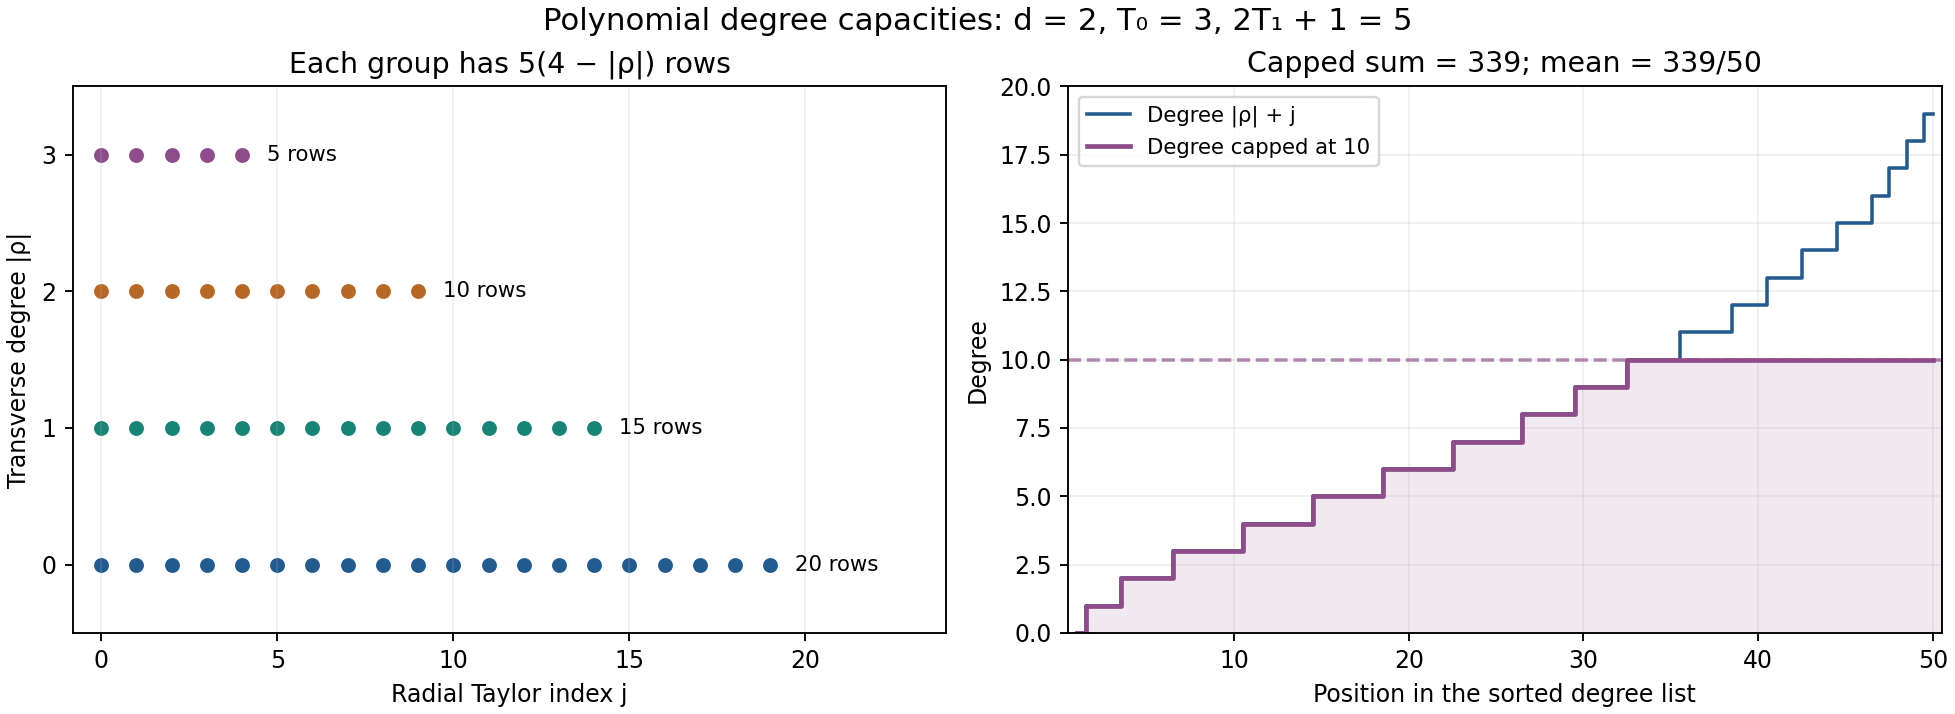
\includegraphics[keepaspectratio,alt={The Taylor-degree capacities and the capped degree list for fifty rows}]{../figures/degree-capacities.png}}
\par\smallskip
\begin{flushleft}\small
\emph{Figure 8.4. For \(d=2\), \(T_0=3\), \(2T_1+1=5\), the four
transverse groups have \(20,15,10,5\) rows. Their lists (8.185) contain
fifty degrees with total \(400\). Capping each at \(z_*=5(3+1)/2=10\)
gives exactly \(339\), so the capped mean is \(339/50>15/4\), as (8.188)
requires. The shaded step diagram represents this exact discrete sum; it
is not an integral approximation. The degree count is independently
supplied above as a refinement of the derivative-determinant mechanism
in {[}Waldschmidt 2000{]}. Source: figures/degree\_capacities.py; exact
arithmetic: verification/degree\_capacity\_parameters.py.}
\end{flushleft}
\end{minipage}\par\medskip


\textbf{Corollary (a stronger finite parameter criterion).} In the
finite parameter proposition, replace (8.183) by \[
\begin{split}
\frac{T_0(2T_1+1)}{m+2}\log E\ge{}&
4DT_0b_1+2(m+1)DS_0b_2+DH+D\log(2L_m)\\
&+(m+1)U
+2(m+1)D(T_1+1)\sum_jS_ja_j.
\end{split}
\tag{8.189}
\] Then the same conclusion (8.184) holds.

\textbf{Proof.} Write \(Z=mV_0=(T_0+1)(2T_1+1)\log E/2\). In the small
rational-line case, (8.182) is strictly stronger: its cost is smaller
than the right side of (8.189), and \(T_0(2T_1+1)\log E/(m+2)<Z\).
Otherwise use the same nonzero minor. Assuming \(0<|\Lambda|\le e^{-Z}\)
gives the same row bounds as in the analytic proof, since \(Z\ge V_d\).
The proof of \(R_d\le M_0\) is unchanged. Apply (8.187)--(8.188), with
\(\varepsilon=\Lambda\). After the same absorption and the derivative
loss \(M_0\log E\), they give \[
\log|\Delta|
<-L\frac{T_0(2T_1+1)}{d+2}\log E+LU_{\rm an}.
\] Because \(d\le m\), condition (8.189) and the arithmetic lower bound
contradict this inequality. Hence \(|\Lambda|>e^{-Z}\). \(\square\)

\subsubsection{Selecting points by their logarithmic
diameter}\label{selecting-points-by-their-logarithmic-diameter}

The hypotheses of Theorem 8.10 bound each logarithm separately. The
following finite-set construction converts these hypotheses into (8.172)
without replacing them by a stronger sum assumption.

\textbf{Lemma (a concentrated part of a symmetric box).} Suppose \[
E|\lambda_j|\le Da_j,\qquad
x_j=\frac{U}{D(T_1+1)a_j}\ge1,\qquad S_j=\lfloor x_j\rfloor.
\] There is a nonempty subset \(A\subseteq\prod_j\{-S_j,\ldots,S_j\}\)
satisfying (8.172), with \[
\#A\ge\frac1{30m}\prod_j(2S_j+1)
>\frac1{30m}\left(\frac32\right)^m
\frac{U^m}{D^m(T_1+1)^m\prod_ja_j}.
\tag{8.190}
\]

\textbf{Proof.} Choose the coordinates \(s_j\) independently and
uniformly in their symmetric integer intervals. Their means are zero.
For \(X=\sum_js_j\lambda_j\), independence gives \[
\mathbb E|X|^2
=\sum_j\mathbb E(s_j^2)|\lambda_j|^2
\le\frac{mU^2}{E^2(T_1+1)^2}.
\] This argument uses complex conjugates in \(|X|^2\), so it applies to
complex logarithms with arbitrary arguments. Markov's inequality, proved
by summing the nonnegative values of \(|X|^2\), shows that at least half
the box lies in \[
|X|\le\frac{\sqrt{2m}\,U}{E(T_1+1)}.
\] In units \(U/(E(T_1+1))\), this disk is inside a square of side
\(2\sqrt{2m}\). Divide each side into
\(Q=\lceil2\sqrt{2m}\rceil<4\sqrt m\) equal intervals. Assign boundary
points consistently to one of the \(Q^2\) cells. Each cell has side at
most one and diameter at most \(\sqrt2<2\). Since \(Q\le2\sqrt{2m}+1\),
we also have \(Q^2\le(9+4\sqrt2)m<15m\). One cell contains at least the
fraction \(1/(2Q^2)>1/(30m)\) of the full box. Its points form the
desired \(A\). There is no translation of their integer coordinates.

Finally \(2\lfloor x\rfloor+1>3x/2\) for every \(x\ge1\). Indeed, for
\(r=\lfloor x\rfloor\ge1\), \(x<r+1\) and \(2r+1\ge3(r+1)/2\).
Multiplying these strict inequalities proves (8.190). \(\square\)

\subsubsection{Parameters for the general algebraic
coefficients}\label{parameters-for-the-general-algebraic-coefficients}

We can now prove (8.154) with its individual logarithmic cutoffs. The
degree-capacity estimate supplies enough room for the finite-set
selection. We keep the coefficient and radius parameters separate.

Write \(m=n\), \(v=\log E\), \(L_B=\log B^*\), \(L_E=\log E^*\), and
\(a_j=\log A_j\). Define \[
r_j=\frac{Da_j}{v},\qquad P=\prod_jr_j,\qquad y=\frac Dv .
\] The hypotheses give \[
r_j\ge1,\quad r_j\le B^*,\quad
L_B\ge L_E\ge1,\quad L_E\ge1/y,\quad y\le e^{L_E}.
\tag{8.191}
\] In this subsection the symbol \(L_B\) is a coefficient logarithm; it
is unrelated to the number of determinant rows.

Choose the following constants: \[
\begin{array}{c|c|c}
 &N&C_0\\ \hline
m=1&48&4\cdot49^2/3\\
m\ge2&4(m+1)^3&
60m(m+1)(N+1)^{m+1}/3^m .
\end{array}
\tag{8.192}
\] Put \[
\begin{aligned}
b_1&=37m^{3/2}L_B,& b_2&=10\sqrt m\,L_E,\\
U&=C_0D^{m+2}b_1b_2\prod_ja_j\,v^{-m-1},&
X&=\frac{U}{Db_1}=C_0b_2yP,\\
T_0&=\lfloor X/2\rfloor,&
T_1&=\lfloor Nyb_1\rfloor,\\
S_0&=\left\lfloor\frac{U}{Db_2}\right\rfloor,&
H&=\left\lfloor\frac{b_1}{6m}\right\rfloor,\\
S_j&=\left\lfloor\frac{U}{D(T_1+1)a_j}\right\rfloor,&
B_i&=e^{b_i}\quad(i=1,2).
\end{aligned}
\tag{8.193}
\] Here \(B_1,B_2\) are auxiliary parameters, not the original \(B^*\).

We verify every finite-parameter hypothesis. First \(C_0\ge100(m+1)\),
\(b_1\ge b_2\), and \[
X\ge10\sqrt m\,C_0\ge1000(m+1),\qquad
yb_1\ge37m^{3/2},\qquad
\frac{b_1}{7m}\le H\le\frac{b_1}{6m}.
\tag{8.194}
\] The last lower bound follows because \(b_1/(6m)>6\); for every real
\(x\ge6\), \(\lfloor x\rfloor\ge6x/7\). The other bounds use
\(yL_E\ge1\), \(P\ge1\), and \(L_B\ge L_E\). All integer parameters are
positive. Moreover \[
T_1+1\le(N+1)yb_1,\qquad
\frac{U}{D(T_1+1)a_j}
\ge\frac{C_0b_2y}{N+1}\prod_{i\ne j}r_i\ge1.
\] Since \(T_1+1>Nyb_1\), the same quotient is smaller than
\(X/(Nr_j)\le X/N\). Thus \(S_j<T_0/4\): indeed \(T_0>X/3\) by (8.194),
and \(N>12\). Also \(S_0+1>U/(Db_2)\ge X\ge2T_0\). The height cutoffs
and \(B_i^D\ge E\) follow from the theorem's hypotheses and
\(b_i\ge L_E\ge v/D\).

For \(m\ge2\), take \(A\) from (8.190). For \(m=1\), take the whole
symmetric interval: \[
A=\{-S_1,\ldots,S_1\}.
\] It already satisfies (8.172), since \(E|\lambda_1|\le Da_1\). In this
case its size exceeds \(3U/(2D(T_1+1)a_1)\). For either choice, the
cardinality condition is equivalent to a strict inequality supplied by
(8.192). Here are the factors explicitly. For \(m\ge2\), (8.190) and
\(S_0+1>U/(Db_2)\) give \[
\frac{(S_0+1)\#A}{2(m+1)T_0^mT_1}
>
\frac{U\,3^m b_1^m}
{60m(m+1)Db_2(T_1+1)^mT_1\prod_ja_j}.
\] Use \(T_1<(N+1)yb_1\) and \(T_1+1\le(N+1)yb_1\); substitution of
\(U\) makes the resulting bound one. For \(m=1\) the same computation
omits the factor \(30m\), and uses \(C_0=2(m+1)(N+1)^{m+1}/3^m\). This
proves the strict rank inequality in both cases.

Next we check the two polynomial-growth requirements (8.173). For the
projective height we will use \[
h(1:\beta'_0:\cdots:\beta'_{m-1})\le(m+1)L_B<b_1,
\tag{8.195}
\] where the normalized coefficients \(\beta'_j\) are defined below. For
the size requirement, the previous bounds on \(S_j\) show \[
T_0S^*\le\frac{m(m+1)}N X^2.
\] Since \(\log y\le L_E\le L_B\), \(\log r_j\le L_B\), and
\(\log L_E\le L_E-1\), we get \[
\log(T_0S^*)
\le
2\log C_0+
\log\frac{100m^3(m+1)}N-2+2(m+2)L_B.
\] Consequently \(T_0S^*3^H\le e^{b_1}\) follows from \[
37m^{3/2}\left(1-\frac{\log3}{6m}\right)
>
2\log C_0+\log\frac{100m^3(m+1)}N-2+2(m+2).
\tag{8.196}
\] This is a uniform inequality. For \(m=1\), its left side exceeds
\(30\), whereas the right side is smaller than \(22\). For \(m\ge2\),
the elementary bounds \[
\log(m+1)\le\sqrt m,\quad
\log(N+1)<1.4+3\sqrt m,\quad
\log60<4.1,\quad \log3>1.09
\] give \(\log C_0<3m^{3/2}+5\sqrt m+0.31m+5.5\). Thus the right side of
(8.196) is smaller than \(6m^{3/2}+11\sqrt m+2.62m+16.3\); its left side
exceeds \(37m^{3/2}-7\sqrt m\). The difference is positive: use
\(\sqrt m\le m\), \(16.3\le8.15m\), and \(31\sqrt m>31\cdot1.4>28.77\).
To justify \(\log(m+1)\le\sqrt m\), put \(x=\sqrt m\ge1\). The ratio
\(e^x/(1+x^2)\) is increasing, since its logarithmic derivative is
\((x-1)^2/(1+x^2)\); at \(x=1\) it exceeds one. All decimal margins used
here are outward rational bounds.

For the other auxiliary parameter, \[
T_1/H\le7mNy,\qquad
\log\{e^2(1+T_1/H)\}
\le2+\log(1+7mN)+L_E.
\] For \(m=1\), \(2+\log337<9\). For \(m\ge2\), \[
2+\log(1+7mN)
\le2+\log29+\log m+3\log(m+1)
<5.4+4\sqrt m<10\sqrt m-1.
\] Since \(L_E\ge1\), these inequalities imply \(B_2\ge e^2(1+T_1/H)\).
We have verified (8.173).

It remains to check the determinant budget (8.189). Its first, second,
fifth and sixth terms together are at most \[
\{2+3(m+1)+2m(m+1)\}U=(2m^2+5m+5)U.
\] The other two terms are smaller than \(U\). Here is a bound which
also checks their dependence on large field degree. Since \(T_0\ge m\)
and \(2(2T_1+1)\le(4N+2)yb_1\le b_1X\), we have \[
2L_m\le X^m b_1X,\qquad
D\log(2L_m)
\le D\{(m+1)X+b_1\}.
\] We used \(C_0b_2\ge4N+2\), which follows at once from (8.192).
Dividing by \(U=Db_1X\) bounds this term by
\((m+1)/b_1+1/X\le2/37+1/X\). Also \(DH/U\le1/(6mX)\). Their sum is less
than one by (8.194). The entire right side of (8.189) is therefore
smaller than \((2m^2+5m+6)U\).

On the left, \(T_0\ge49X/100\) and \(2T_1+1\ge(2N-1)yb_1\), so \[
\frac{T_0(2T_1+1)v}{m+2}
\ge\frac{49(2N-1)}{100(m+2)}U
>(2m^2+5m+6)U.
\] For \(m=1\), the coefficient on the left is \(4655/300>13\). For
\(m\ge2\), clearing denominators reduces the last inequality to \[
192m^3+276m^2-424m-857>0.
\] Its value at \(m=2\) is \(935\); after putting \(m=2+x\), its
remaining coefficients are \(2984,1428,192\), all positive. This proves
the required budget without an asymptotic argument.

We can now finish the coefficient normalization. If all coefficients of
the logarithms are zero, the nonzero constant \(\Gamma=\beta_0\) has
\(\log|\Gamma|\ge-DL_B\) by Liouville. Otherwise permute the logarithms
so that \(\beta_m\ne0\), and put \[
\beta'_j=-\beta_j/\beta_m\quad(0\le j<m),\qquad
\Lambda=\beta'_0+\sum_{j<m}\beta'_j\lambda_j-\lambda_m.
\] Then \(\Gamma=-\beta_m\Lambda\). The projective-height identities
give (8.195), and \(\log|\beta_m|\ge-DL_B\). Baker's full theorem in the
preceding third lesson, including the constant term, gives
\(\Gamma\ne0\). Rational independence of the chosen logarithms also
implies that the multiplicative group of the \(\alpha_j\) has free rank
at least \(m-1\). Indeed, two independent integer relations modulo
torsion would give two rational multiples of \(2\pi i\) as logarithmic
sums; eliminating them gives a nonzero rational relation among the
\(\lambda_j\). Thus every hypothesis of the stronger finite proposition
is satisfied.

Its conclusion and the rounding bounds in (8.193) give \[
\begin{split}
\log|\Gamma|>{}&
-\left\{\frac{370m^2(2N+1)(C_0+2)}4+1\right\}
D^{m+2}\prod_ja_j\,
\frac{L_BL_E}{v^{m+1}}.
\end{split}
\tag{8.197}
\] For the added coefficient cost, use \[
D^{m+2}\prod_ja_j\,L_BL_E\,v^{-m-1}
=D\,yP L_BL_E\ge DL_B.
\] For the determinant cost use \(T_0+1\le X/2+1\),
\(2T_1+1\le(2N+1)yb_1\), and \(X\ge C_0\).

Finally the constant in braces is strictly smaller than
\(2^{m+25}m^{3m+9}\). For \(m=1,2,3\) this follows by direct integer
arithmetic in (8.192); the ratios are respectively less than
\(0.429,0.947,0.478\). For \(m\ge4\), first observe \[
\frac{370m^2(2N+1)(C_0+2)}4+1
<186m^2(N+1)C_0.
\] The difference already exceeds one for \(m\ge2\), since \(C_0>10^6\).
Use \(N+1<(81/20)(m+1)^3\), and divide by the target constant. The
result is at most \[
\frac{11160(81/20)^2}{2^{25}}\,
m(1+1/m)^{3m+7}(27/40)^m
<
0.00546\cdot21(5/4)^7\,m(27/40)^m<0.46.
\] Here \((1+1/m)^{3m}<e^3<21\). The sequence \(m(27/40)^m\) decreases
for \(m\ge4\), because its successive ratio is at most \(27/32<1\); its
first value is \(4(27/40)^4\). This proves the comparison for every
dimension. Equation (8.197) establishes (8.154) in the full
algebraic-coefficient, rationally independent case. The proof uses the
same rank, height and derivative construction as {[}Waldschmidt 2000{]};
the degree-capacity count and symmetric-box selection above give the
explicit parameter transfer used here.

\subsubsection{Integer coefficients and binomial
polynomials}\label{integer-coefficients-and-binomial-polynomials}

The homogeneous bound has a smaller coefficient parameter than a general
projective height. We retain it by choosing a polynomial basis which
takes integer values at the interpolation points.

For \(z\in\mathbb C\), set \[
\binom zr=\frac{z(z-1)\cdots(z-r+1)}{r!},\qquad \binom z0=1.
\] For every integer \(z\), these values are integers. For \(z\ge0\)
this follows by counting subsets (with zero if \(r>z\)); for \(z<0\),
the identity \(\binom zr=(-1)^r\binom{r-z-1}{r}\) proves it.

We also need their growth. If \(Z_i\ge0\), \(|z_i|\le Z_i\),
\(r_i\ge0\), and \(r=\sum_ir_i\le T\), \(T\ge1\), then \[
\prod_i\left|\binom{z_i}{r_i}\right|
\le\left\{e\left(1+\frac{\sum_iZ_i}{T}\right)\right\}^{T}.
\tag{8.198}
\] For \(r_i>0\), each numerator factor has modulus at most \(Z_i+r_i\).
Also \(r_i!\ge(r_i/e)^{r_i}\), by integrating \(\log x\) over
\(1\le x\le r_i\). Thus the product is at most \[
\prod_{r_i>0}\{e(1+Z_i/r_i)\}^{r_i}
\le\{e(1+\sum_iZ_i/r)\}^{r}.
\] The last inequality is the weighted arithmetic--geometric mean,
applied with weights \(r_i/r\). The function \(r\log\{e(1+Z/r)\}\) is
increasing for \(r>0\): its derivative is \(1+\log(1+Z/r)-Z/(r+Z)>0\).
Increase \(r\) to \(T\) to obtain (8.198); the case \(r=0\) is
immediate.

Let \(b_j\in\mathbb Z\), \(b_m\ne0\), and normalize \[
\beta_0=0,\qquad \beta_j=-b_j/b_m\ (j<m),\qquad
\Lambda=-\frac1{b_m}\sum_jb_j\lambda_j.
\] In the minimal subspace of dimension \(d\), replace the monomials by
\[
p_\tau(X)=\frac{X_0^{\tau_0}}{\tau_0!}
\prod_{i=m-d+1}^{m-1}\binom{b_mX_i}{\tau_i},
\qquad |\tau|\le T_0.
\tag{8.199}
\] These form a basis of all polynomials of degree at most \(T_0\):
their leading monomials have nonzero coefficients, and ordering by total
degree makes the change-of-basis matrix triangular. The rank proposition
therefore supplies a nonzero minor for this basis too. Its number of
rows and its logarithmic Laurent support are unchanged.

For \(s\in(A-A)[m+1]\), define the integers \[
z_i(s)=b_ms_i-b_is_m,\qquad
Z_i=2(m+1)(|b_m|S_i+|b_i|S_m).
\] The first coordinate \(y_0(s)\) is zero. Evaluation after
differentiation gives the algebraic entry \[
M_{\tau t,\sigma s}
=\alpha^{ts}\,
\frac{q_\sigma^{(\tau_0)}(t)}{\tau_0!}
\prod_{i=m-d+1}^{m-1}\binom{z_i(s)}{\tau_i}.
\tag{8.200}
\] To check the factor, differentiate \(X_0^{\tau_0}e^{tX_0}/\tau_0!\)
at zero. In \(q_\sigma(\partial_{X_0})\), the resulting coefficient is
exactly \(q_\sigma^{(\tau_0)}(t)/\tau_0!\). All binomial factors in
(8.200) are integers. The normalized denominator lemma therefore clears
its row by \(\nu^{\tau_0}\), \(\nu=\operatorname{lcm}(1,\ldots,H)\).

For example, let \(b_m=3\), \(b_i=2\), \(s_i=2\), \(s_m=-1\). Then
\(b_ms_i-b_is_m=8\), so the transverse factor with \(\tau_i=3\) is
\(\binom83=56\). Take \(\tau_0=2\), \(t=0\), and \(q(z)=z(z+1)(z+2)/6\).
Its normalized derivative \(q''(0)/2!\) is \(1/2\), so this scalar entry
is \(28\). Applying \((\partial^3+3\partial^2+2\partial)/6\) directly to
\(X_0^2/2!\) at zero gives the same \(1/2\). This illustrates why
differentiation occurs before evaluation at the zero first coordinate.

In place of the projective height and size conditions for \(B_1\), it
suffices that \[
B_1\ge3^H,\qquad
B_1\ge e+\frac{2em(m+1)}{T_0}
\max_{j<m}(|b_m|S_j+|b_j|S_m).
\tag{8.201}
\] Use zero for the maximum when \(m=1\). Indeed,
\(\sum_iZ_i\le2m(m+1)\max_{j<m}(|b_m|S_j+|b_j|S_m)\). Equations (8.198)
and (8.201) bound the binomial product by \(B_1^{T_0}\), and by
\((EB_1)^{T_0}\) at radial arguments \(z\,y(s)\) with \(|z|=E\). There
is no projective-height factor: the integer coefficient combinations are
evaluated before applying the product formula.

Here are the resulting determinant bounds explicitly. The polynomial
derivative estimate bounds \(q_\sigma^{(\tau_0)}(t)/\tau_0!\) by
\(e^{H-M_0}B_2^{M_0}\). After denominator clearing, every algebraic
scalar entry has modulus at most \[
e^{H-M_0}B_1^{2T_0}B_2^{M_0}.
\] Expanding the determinant gives an integer Laurent polynomial in the
\(\alpha_j\). Its coefficient length is at most \(L!\) times the
\(L\)-th power of this bound. The product formula costs at most \(D-1\)
times its logarithmic coefficient length. Subtracting the clearing
denominator costs at most \[
\frac{LT_0}{d+1}\log\nu\le\frac{LT_0}{d+1}b_1.
\] Thus its coefficient contribution is at most
\((2D-2+1/(d+1))LT_0b_1\), which is no larger than \((2D-1)LT_0b_1\).
The height contribution of the \(\alpha_j\) is exactly bounded as in
(8.176). Dropping the favorable \(-M_0\) proves the same arithmetic
lower bound (8.174)--(8.175).

On the analytic circle the scalar part is bounded by \[
e^{H-M_0}B_1^{T_0}B_2^{M_0}E^{T_0}.
\] The exponential factor, perturbation identity and \(R_d\le M_0\) are
the same as before. The degree-capacity argument applies to any basis of
the polynomial space, including (8.199). It gives the same stronger
analytic estimate, with the smaller coefficient cost \(T_0(b_1+v)\). In
particular the more conservative \(U_{\rm an}\) in (8.180) still bounds
it. Consequently the stronger finite criterion (8.189) and the
small-rational-line alternative remain valid under (8.201); no
coefficient-height assumption is needed.

To prove (8.155), set \[
L_B=2\log B',\qquad L_E=\log E^*,
\] and use all constants and integer parameters (8.192)--(8.194). These
now satisfy \(L_B\ge L_E\ge1\), but no assumption \(r_j\le e^{L_B}\) is
imposed or used. The positive cutoffs, coordinate bounds, rank
cardinality, \(B_2\) growth, determinant budget and final constant
comparison in the preceding proof use only \(r_j\ge1\) and \(P\ge1\);
they therefore still apply. Only the \(B_1\) check is replaced. Its
first condition follows from \(H\le b_1/(6m)\). For the second, the
definition of \(B'\) gives \[
\max_{j<m}(|b_m|S_j+|b_j|S_m)
\le\frac{UB'}{D(T_1+1)}.
\] Since \(T_0\ge49X/100\) and \(T_1+1>Nyb_1\), the right side required
in (8.201) is at most \[
e+\frac{200em(m+1)}{49N}\frac{B'}y.
\] For \(m\ge2\), \(N=4(m+1)^3\), so \(200em(m+1)/(49N)<1\): use \(e<3\)
and \(m/(m+1)^2\le2/9\). For \(m=1\), the maximum is empty. Moreover
\(1/y=v/D\le\log B'\le B'\), since \(B'\ge E^*\ge E^{1/D}\). Thus for
\(m\ge2\) the required bound is smaller than \(e+(B')^2\le(B')^3\), as
\(B'\ge e>2\). Our choice \(B_1=(B')^{74m^{3/2}}\) is larger still. This
proves (8.201).

Finally \(|\sum_jb_j\lambda_j|=|b_m\Lambda|\ge|\Lambda|\), since \(b_m\)
is a nonzero integer. There is no additional coefficient cost. The
constant comparison already proved for (8.197), with \(L_B=2\log B'\),
yields exactly (8.155). This completes the homogeneous estimate under
rational independence. The integer-valued basis mechanism is credited to
{[}Waldschmidt 2000{]}; all growth, denominator and parameter arguments
used here have been supplied above.

\subsubsection{Relation coefficients adapted to the
radius}\label{relation-coefficients-adapted-to-the-radius}

The coefficient cost in a dependent family must be bounded together with
the chosen logarithms. We give an estimate that uses their small
modulus. Put \[
v=\log E,\quad u=\log E^*,\quad y=D/v,\quad t_j=ya_j\ge1.
\] Thus \(u\ge1\), \(yu\ge1\), and \(y\le e^u\). These inequalities hold
in both versions of Theorem 8.10.

First let \(e^\lambda=\gamma\in K^\times\), \(\lambda\ne0\), and let
\(M\ge1\) be an integer for which \(\gamma,\ldots,\gamma^M\ne1\). Then
\[
-\log|\lambda|
\le\frac{D(M+2)}3h(\gamma)
+\frac D M\log(M+1)+\log M+\frac{M+2}3|\lambda|.
\tag{8.202}
\]

\textbf{Proof.} Define \[
Q_M(Z)=\prod_{j=1}^M(Z^j-1)^{M+1-j},\qquad
s_0=\frac{M(M+1)}2,\quad s_1=\frac{M(M+1)(M+2)}6.
\] On the unit circle the modulus of \(Q_M\) equals that of the
Vandermonde determinant on \(1,Z,\ldots,Z^M\). Each row has norm
\(\sqrt{M+1}\), so Hadamard's inequality bounds it by
\((M+1)^{(M+1)/2}\). The maximum principle gives the same bound inside
the unit disk. The identity \(|Q_M(Z)|=|Z|^{s_1}|Q_M(Z^{-1})|\) then
gives \[
|Q_M(Z)|\le(M+1)^{(M+1)/2}\max\{1,|Z|\}^{s_1}.
\] At finite places the bound holds without the fixed factor, because
this polynomial has integer coefficients. Since \(Q_M(\gamma)\ne0\), the
product formula gives \[
\log|Q_M(\gamma)|\ge-Ds_1h(\gamma)
-\frac{D(M+1)}2\log(M+1).
\] Using \(D\) for the other archimedean embeddings only weakens the
inequality. The bound \(|e^{j\lambda}-1|\le j|\lambda|e^{j|\lambda|}\),
summed with weights \(M+1-j\), gives \[
\log|Q_M(\gamma)|\le s_0\log|\lambda|+s_0\log M+s_1|\lambda|.
\] Compare and divide by \(s_0\). This proves (8.202). \(\square\)

This is the elementary Vandermonde and product-formula mechanism of
(8.23), arranged to retain a very small chosen logarithm.

\textbf{Lemma (a radius-dependent empty body).} Let \(C\) be the
absolute convex hull of \(v(\alpha_j,\lambda_j)/a_j\) in (8.11), for any
family meeting the height and chosen-logarithm cutoffs. Let
\(\mathcal L\) be a discrete subgroup of logarithmic vectors in their
span, all coming from bases in \(K\). There is no nonzero point of
\(\mathcal L\) in \(\eta C\), where \[
\eta=
\begin{cases}
(11D^3)^{-1},&\log D\le16u,\\[2mm]
\min\{1,(64yM)^{-1}\},&\log D>16u,\quad M=\lceil64yu\rceil .
\end{cases}
\tag{8.203}
\]

\textbf{Proof.} A point \(v(\gamma,\lambda)\in\delta C\) satisfies \[
h(\gamma)\le\delta,\qquad |\lambda|\le D\delta e^{-v}.
\tag{8.204}
\] The height formula and the triangle inequality in the logarithmic
coordinates prove the first inequality. The selected real and imaginary
coordinates prove the second. Both hold on the whole absolute convex
hull.

If \(\log D\le16u\), a nontorsion base has height greater than
\(1/(11D^3)\) by (8.1). For a torsion base of order \(q\), the bound
\(q\le2D^2\) proved above implies \(|\lambda|\ge\pi/D^2\) for a nonzero
chosen logarithm. This exceeds the bound in (8.204). A nonzero period of
the base one is included.

Otherwise write \(L=\log D>16u\), \(x=L-u>15u\). The radius hypotheses
give \[
v\ge e^{L-u}=e^x>4L+28u+4.
\] Indeed \(4L+28u+4=4x+32u+4<7x+4\); \(e^x-7x-4\) is positive and
increasing for \(x\ge15\). At fifteen, use \(e^{15}>2^{15}>109\).

Suppose a nonzero point lies in \(\eta C\). Its chosen logarithm is
nonzero by (8.11). It cannot have a torsion base, since \[
|\lambda|\le De^{-v}<D^{-3}<\pi/D^2.
\] Thus (8.202) applies. We have \[
64yu\le M\le65yu,\quad M\ge64,\quad
\log(M+1)\le\log(66yu)<5+2u\le7u.
\] Here \(\log y\le u\), \(\log u\le u\), and \(yu\ge1\). The first two
terms in (8.202) are at most \[
\frac v{192}(1+2/M),\qquad \frac{7v}{64},
\] whose sum is less than \(v/8\). Also \(\log M\le7u\), and
\(\log(MD)\le L+7u<v/2\), so \((M+2)|\lambda|/3\le MDe^{-v}<1\).
Therefore (8.202) gives \(-\log|\lambda|<v/8+7u+1\). But (8.204), with
\(\eta\le1\), gives \(-\log|\lambda|\ge v-L\). These are incompatible
with \(v>4(L+7u+1)\). This proves the lemma. \(\square\)

\textbf{Lemma (a primitive circuit with logarithmic cost).} Choose a
minimally dependent subset \(J\) of nonzero chosen logarithms, of size
\(q\ge2\), and choose \(k\in J\) with \(a_k=\max_{j\in J}a_j\). There is
a primitive relation \(\sum_{j\in J}c_j\lambda_j=0\), with every
\(c_j\ne0\). Set \(c_j=0\) outside \(J\) and \(N=\max_j|c_j|\ge1\). For
an ambient family of \(n\ge q\) terms, \[
\log N\le64n^2u\,t_k,\qquad t_k=Da_k/v.
\tag{8.205}
\]

\textbf{Proof.} Use \(C\) from (8.203) for \(J\), and let \(\mathcal L\)
be generated by its logarithmic vectors. It is discrete by (8.11), and
has real rank \(r=q-1\): a discrete spanning group has an integer basis,
so its real rank equals its rational rank. Minkowski's first theorem and
(8.203) give \[
\eta^r\operatorname{vol}_r C\le2^r\det\mathcal L.
\] For each \(j\in J\), the cross-polytope on the other \(r\) vectors
divided by their cutoffs lies in \(C\). Its volume is \(2^r/r!\) times
their absolute determinant. In an integer basis of \(\mathcal L\), the
primitive relation coefficients are the signed maximal minors. Their
greatest common divisor is one because the columns generate
\(\mathcal L\), by the Smith reduction proved above. It follows that \[
|c_j|\le r!\eta^{-r}\prod_{i\in J\setminus\{j\}}a_i,
\qquad N\le r!(a_k/\eta)^r.
\]

If \(L=\log D\le16u\), then \[
\log(a_k/\eta)=\log11+3L+\log t_k-\log y
<52u+\log t_k,
\] since \(-\log y\le\log u\le u\) and \(u\ge1\). Using \(r!\le r^r\),
\(\log t_k\le t_k\), and \(t_k\ge1\), we obtain
\(\log N<r(\log r+53)u t_k\le64n^2u t_k\). For the last comparison use
\(r<n\), \(\log r\le r\), \(n\ge2\).

If \(L>16u\), then \(\eta^{-1}=\max\{1,64yM\}\). When \(64yM\ge1\),
\(a_k/\eta\le4160yu\,t_k\), whence \(\log(a_k/\eta)<11u+\log t_k\). When
\(64yM<1\), instead \(a_k/\eta=t_k/y\le u t_k\), giving a smaller
logarithmic bound. Thus \(\log N<r(\log r+12)u t_k\), which also proves
(8.205). \(\square\)

The estimate controls the actual primitive relation together with the
radius, rather than a degree-only upper bound.

\subsubsection{Completing the dependent algebraic-coefficient
estimate}\label{completing-the-dependent-algebraic-coefficient-estimate}

Write \[
C_n=2^{n+25}n^{3n+9},\quad P=\prod_jt_j,\quad
w=\log B^*,\quad \Phi_n=C_nD ywuP.
\] This is exactly the magnitude of the exponent in (8.154). For
\(n\ge2\), \[
C_n/C_{n-1}>2(64n^2+4),\qquad C_n>128n^2.
\tag{8.206}
\] For \(n=2,3\) these are exact integer comparisons. For \(n\ge4\), \[
C_n/C_{n-1}
=2n^3(n/(n-1))^{3n+6}>2e^3n^3>40n^3>2(64n^2+4).
\] The bound \(\log(1+s)\ge s/(1+s)\), \(s>0\), proves the first strict
estimate. The polynomial \(20n^3-64n^2-4\) is positive at four and
increasing thereafter. The second assertion follows directly from the
formula.

We prove (8.154) by induction on the number of terms, assuming only
\(\Gamma\ne0\). For independent logarithms the full estimate is (8.197).
A zero logarithm can be deleted with unchanged coefficients,
\(B^*,E,E^*\); its lost factor \(t_j\ge1\) and the increasing constant
make the smaller estimate stronger. Use the original \(D\) as a degree
upper bound for the smaller generated field. In (8.174)--(8.176),
replacing its actual degree by \(D\) only increases the nonnegative
arithmetic costs. The rank and analytic estimates do not require
equality of the degrees; the choices (8.191)--(8.196) use this same
upper bound throughout. Thus the completed independent proof applies
with these parameters. If every logarithmic contribution is zero,
Liouville gives \(\log|\Gamma|\ge-Dw>-\Phi_n\), since \(yu\ge1\) and
\(P\ge1\). This also covers a single zero logarithm in the base case.

For nonzero dependent logarithms use the circuit (8.205), delete its
largest-cutoff index \(k\), and set \[
\beta'_0=c_k\beta_0,\qquad
\beta'_j=c_k\beta_j-c_j\beta_k\quad(j\ne k).
\] The new form is exactly \(c_k\Gamma\ne0\). The height inequalities
give \(h(\beta'_j)\le2w+\log(2N)\) and \(h(\beta'_0)\le w+\log N\).
Choose \[
w'=\max\{u,\max_{j\ne k}\log t_j,\;2w+\log(2N)\},
\qquad B_{\rm new}^*=e^{w'}.
\] It meets all smaller-dimensional hypotheses. Since \(w\ge u\ge1\),
(8.205) gives \(w'\le(64n^2+3)w t_k\). Induction and (8.206) give a
smaller exponent \[
\Phi'_{n-1}=C_{n-1}D y w'uP/t_k<\Phi_n/2.
\] Moreover \[
\log|c_k|\le\log N\le64n^2u t_k
\le(64n^2/C_n)\Phi_n<\Phi_n/2,
\] using \(D y w\ge1\) and \(P\ge t_k\). Thus \[
\log|\Gamma|
=\log|c_k\Gamma|-\log|c_k|
\ge-\Phi'_{n-1}-\log|c_k|>-\Phi_n.
\tag{8.207}
\] This completes the algebraic-coefficient reduction.

\subsubsection{Completing the homogeneous coefficient
estimate}\label{completing-the-homogeneous-coefficient-estimate}

Put \(w=\log B'\), and double \(C_n\) in \(\Phi_n\). The constant ratios
are unchanged. We retain the exact normalized parameter in (8.155).

Deleting a nondistinguished zero logarithm does not increase \(B'\). If
the distinguished logarithm is zero, select a surviving nonzero
contribution as the new last term. Every other original coefficient
satisfies \(|b_j|\le B'a_n\), and every reciprocal cutoff is at most
\(y\). The new parameter, including its floor \(E^*\), is therefore at
most \(2B't_n\), with logarithm at most \(3w t_n\). The constant ratio
absorbs this cost. The nonzero one-term case is the independent theorem.

For a dependent family use the same primitive circuit, delete the
largest cutoff in its support, and put \[
b'_j=c_kb_j-c_jb_k\quad(j\ne k),\qquad
c_k\Lambda=\sum_{j\ne k}b'_j\lambda_j.
\] There is a surviving nonzero coefficient. With an appropriate
distinguished term, \[
B'_{\rm new}\le4NB't_k.
\tag{8.208}
\]

If \(k=n\), choose any surviving nonzero coefficient as the new last
one. For two surviving indices \(i,q\), the original bounds
\(|b_j|\le B'a_n\) and \(|b_n|/a_j\le B'\) give \[
|b'_q|/a_i+|b'_i|/a_q
\le2NB'(1+t_n)\le4NB't_n.
\] If only one term survives, the normalized maximum is empty.

If \(k\ne n\) and \(b'_n\ne0\), keep \(n\) distinguished. For
\(i\ne k,n\), \[
|b'_n|/a_i+|b'_i|/a_n\le NB'(3+t_k).
\] Indeed the three ordinary terms are bounded by \(B'\). The extra term
involving \(c_n b_k/a_i\) is absent if \(c_n=0\). Otherwise \(n\)
belongs to the circuit, \(a_n\le a_k\), and
\(|b_k|/a_i\le B'a_n y\le B't_k\).

If \(b'_n=0\), then \(c_n b_k=c_kb_n\ne0\), so again \(a_n\le a_k\).
Every remaining original nondistinguished coefficient has
\(|b'_j|\le2NB'a_n\). Choose a nonzero one as the new distinguished
term. Both reciprocal cutoffs are at most \(y\), giving normalized sum
at most \(4NB'a_n y\le4NB't_k\). The original distinguished coefficient
is zero and obeys the same bound. Finally \(E^*\le B'\le4NB't_k\). This
proves (8.208) in all cases.

Consequently \[
w'\le w+\log4+\log N+\log t_k
\le(64n^2+4)w t_k.
\] Induction gives an exponent less than half the original one. The
multiplier costs less than the other half, exactly as in (8.207), now
with the doubled constant. This proves (8.155) for every dependent
family with \(\Lambda\ne0\). \(\square\)

Both conclusions required under (8.156) now have their original
constants and coefficient parameters. The radius-adapted relation
argument actually proves them from nonvanishing alone, without using
(8.156). This strengthening belongs to the proof here; the cited
statement of {[}Waldschmidt 2000{]}, retains its published additional
hypothesis. The verification script
\href{../verification/waldschmidt_dependent.py}{waldschmidt\_dependent.py}
checks finite identities and constant endpoints.

\begin{minipage}[t]{\linewidth}
\centering
\pandocbounded{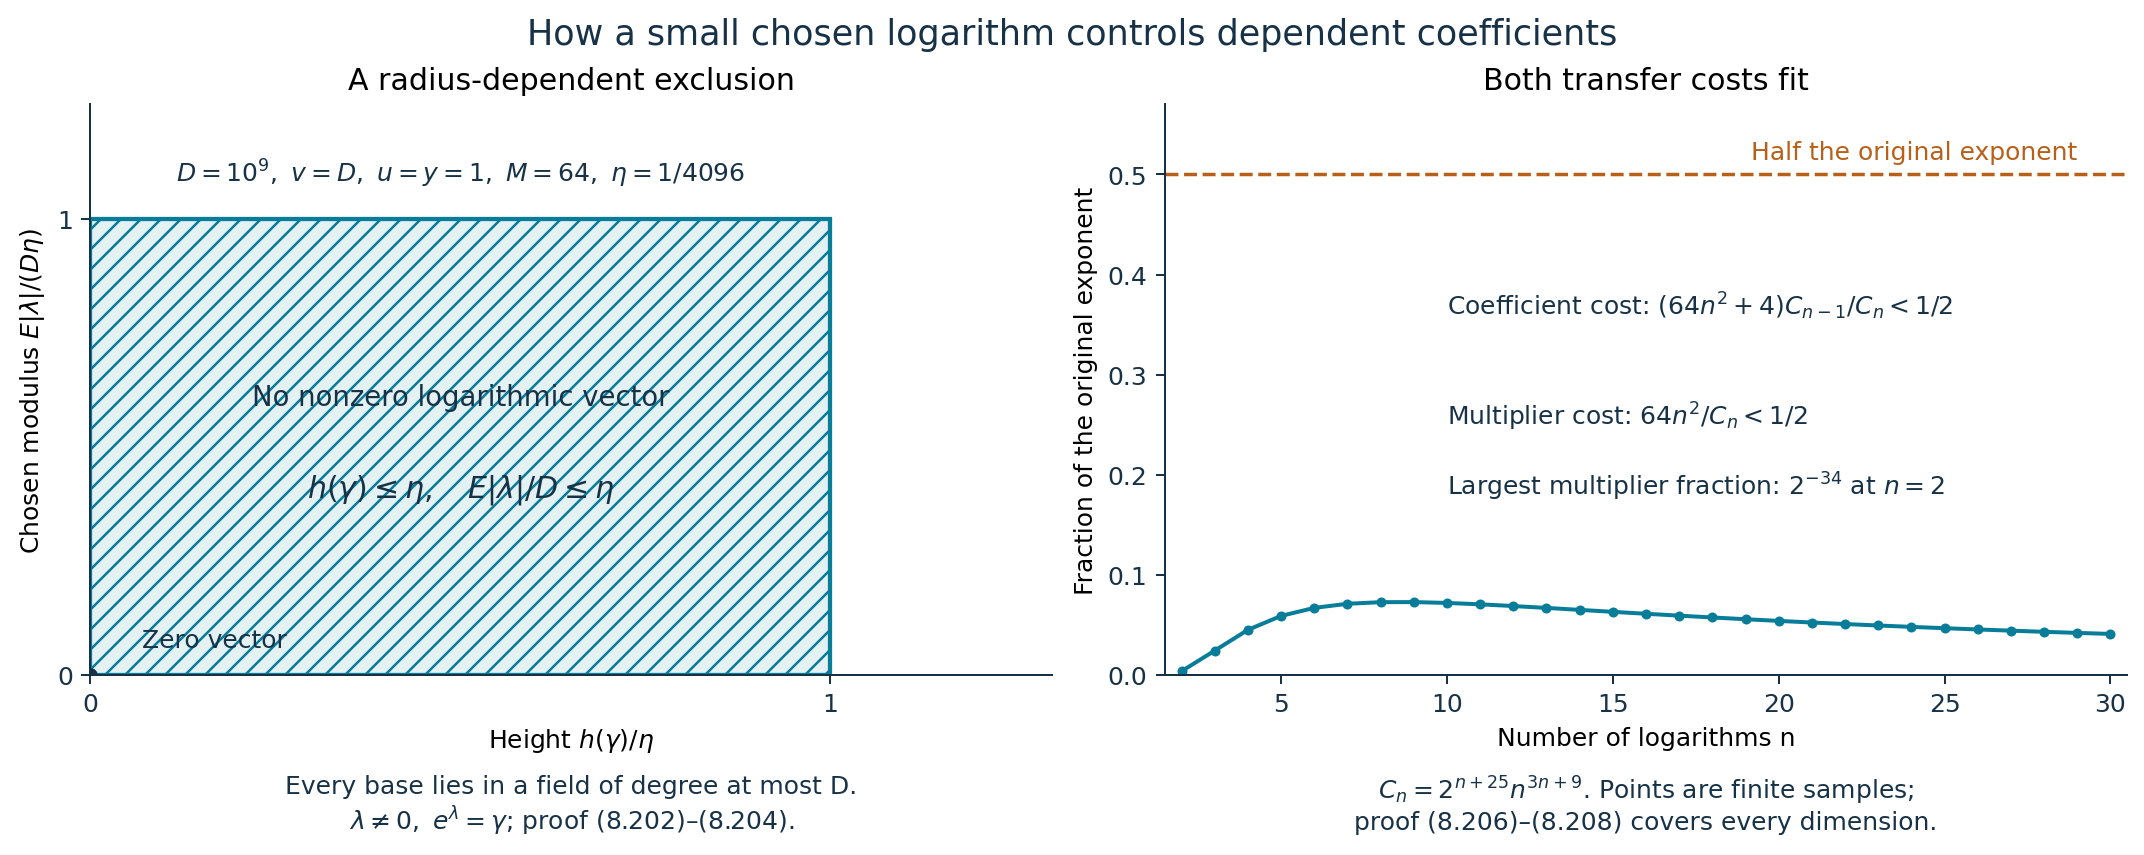
\includegraphics[keepaspectratio,alt={The radius-dependent exclusion and the two coefficient-transfer costs}]{../figures/radius-adapted-circuit.png}}
\par\smallskip
\begin{flushleft}\small
\emph{Figure 8.5.}
\end{flushleft}
\end{minipage}\par\medskip
 On the left, \(D=10^9\), \(v=D\), \(u=y=1\), and
\(E=e^v\). The normalized square expresses the proved exclusion
(8.202)--(8.204); it does not plot conjugates of a particular number
field. The zero logarithmic vector is allowed at the origin. On the
right, finite samples illustrate the exact ratios bounded in
(8.206)--(8.208). The multiplier fraction is largest at \(n=2\), where
it equals \(2^{-34}\): (8.206) makes \(n^2/C_n\) decrease. Both proofs
cover every dimension. The Vandermonde/product-formula mechanism is
credited as in (8.23); the radius-dependent construction and figure are
supplied here.
\href{../verification/radius_adapted_circuit_figure.py}{Reproducible
figure source}.

\textbf{Example (both coefficient parameters).} Take \(K=\mathbb Q\),
\((\alpha_1,\alpha_2,\alpha_3)=(2,3,6)\), their real logarithms,
\(E=E^*=e\), and \((a_1,a_2,a_3)=(2,3,5)\). These satisfy all three
cutoffs: \(e\log2<2\), \(e\log3<3\), and \(e\log6<5\). For \[
\Gamma=1+2\log2-3\log3+4\log6
      =1+6\log2+\log3,
\] the algebraic-coefficient parameter \(B^*=5\) is valid. The primitive
circuit is \((1,1,-1)\). Deleting its largest cutoff gives
\(\beta'_0=-1\), \((\beta'_1,\beta'_2)=(-6,-1)\), and the transformed
form equals \(-\Gamma\). One may use the exact smaller parameter
\(B^*_{\rm new}=6\).

For the homogeneous form with coefficients \((2,-3,4)\), the original
normalized maximum is \(12/5<e\), so \(B'=e\). The same elimination has
normalized maximum \(1/2+6/3=5/2<e\); thus \(B'_{\rm new}=e\) also
works. The general bound (8.208) allows growth of the parameter, but
this exact example shows that growth is not necessary. Both forms are
nonzero by their displayed positive expressions.

\subsection{9. Why a large radius helps}\label{why-a-large-radius-helps}

Take rational bases \[
\alpha_j=1+\frac1{x_j},\qquad x_j\in\mathbb Z,\quad x_j\ge3.
\] Their reduced fractions have height \(h(\alpha_j)=\log(x_j+1)\). Set
\[
X=\min_jx_j,\quad E=E^*=X,\quad a_j=\log(x_j+1).
\] These choices satisfy every radius and height requirement:
\(X\ge3>e\), \[
E\log(1+1/x_j)<E/x_j\le1<a_j,\qquad
\log E\le a_j.
\] The field degree is one, so condition (8.156) is automatic for any
nonzero form. For \(b_n\ne0\), put \(B=\max_j|b_j|\ge1\). If \(B\ge X\),
the choice \(B'=2B\) is permitted, because \(a_j>1\) and \[
\frac{|b_n|}{a_j}+\frac{|b_j|}{a_n}<2B.
\] Thus (8.155) becomes \[
\log\left|\sum_jb_j\log(1+1/x_j)\right|
\ge-2^{n+26}n^{3n+9}
\frac{\prod_j\log(x_j+1)}{(\log X)^n}\log(2B). \tag{8.209}
\] For example, if \(X\le x_j\le X^M\), \(M\ge1\), then \[
\frac{\log(x_j+1)}{\log X}
\le M+\frac{\log(4/3)}{\log3}<1.263M.
\] The height quotient in (8.209) is therefore at most \((1.263M)^n\).
The degree-one radius has removed the large factor \((\log X)^n\) that
the product of unmodified height cutoffs would contribute.

The restriction \(B\ge X\) in this simplified formula is essential; the
original theorem always retains \(B'\ge E^*\). To see the reason, take
two consecutive denominators, \(x_1=N\), \(x_2=N+1\), and coefficients
\(1,-1\). The bases are multiplicatively independent. A prime dividing
\(N+1\), which is coprime to both \(N\) and \(N+2\), would force equal
coefficients in a multiplicative relation; their product would then be
\(((N+2)/N)^b=1\), forcing \(b=0\). Their form is \[
\log\frac{N+1}{N}-\log\frac{N+2}{N+1}
=\log\left(1+\frac1{N(N+2)}\right).
\] For \(t>0\), integration of \(1/(1+t)\) gives \[
\frac t{1+t}\le\log(1+t)\le t.
\] The form consequently lies between \(1/(N+1)^2\) and \(1/(N(N+2))\),
and its logarithm is \(-2\log N+o(1)\). Here \(B=1\), so the admissible
coefficient parameter is \(B'=N\), not a fixed constant. Its logarithm
correctly retains the dependence on \(N\).

\subsection{10. The conjectural height
dependence}\label{the-conjectural-height-dependence}

The product of height cutoffs is a proved feature of (8.145), (8.147)
and (8.155). Replacing it by an additive height expression would have
much stronger consequences. We state the precise integer-base
formulation discussed in the freely accessible author text
{[}Waldschmidt 2000{]}.

\textbf{Conjecture (Lang--Waldschmidt).} For each \(\varepsilon>0\),
there is a number \(c(\varepsilon)>0\) such that, for every \(n\ge1\)
and nonzero integers \(a_1,\ldots,a_n,b_1,\ldots,b_n\) with
\(P=\prod a_j^{b_j}\ne1\), \[
|P-1|\ge
\frac{c(\varepsilon)^n}
{B^{n-1+\varepsilon}A^{n+\varepsilon}},
\quad
A=\max\{2,|a_1|,\ldots,|a_n|\},\
B=\max\{2,|b_1|,\ldots,|b_n|\}. \tag{8.210}
\] No effectivity of \(c(\varepsilon)\) is asserted.

Taking negative logarithms would give \[
-\log|P-1|\le
(n-1+\varepsilon)\log B+
(n+\varepsilon)\log A-n\log c(\varepsilon).
\] The height contribution would be linear in \(\log A\) for fixed
\(n\), whereas the proved general estimate includes a product of \(n\)
logarithmic heights. An estimate using a sum of individual logarithmic
heights would have the same qualitative advantage, but its precise
quantifiers and constants must also be supplied; it should not be
conflated with a proved theorem.

\textbf{Proposition 8.11 (conditional gaps).} If (8.210) holds, then for
a finite prime set \(S\) of cardinality \(s\), and every
\(\varepsilon>0\), there is \(c_{S,\varepsilon}>0\) such that distinct
positive integral \(S\)-units \(2\le u<v\) satisfy \[
v-u\ge
c_{S,\varepsilon}\,
\frac{u}{(\log(2u))^{s-1+\varepsilon}}. \tag{8.211}
\] The constant is not asserted to be effective.

\textbf{Proof.} If \(v\ge2u\), the gap is at least \(u\), so (8.211)
holds with \(c_{S,\varepsilon}\le1\), since \(\log(2u)>1\). Otherwise
express \(v/u=\prod_{p\in S}p^{v_p-u_p}\), and discard zero exponents.
If \(k\) remain, then \(1\le k\le s\); the exponent parameter in (8.210)
is at most \[
B_0=\max\left\{2,\frac{\log(2u)}{\log2}\right\}
\le\frac{2\log(2u)}{\log2}.
\] Let \(A_0=\max S\) and \(c_0=\min\{1,c(\varepsilon)\}\). The
conjecture gives \[
\frac vu-1\ge
\frac{c_0^s}{A_0^{s+\varepsilon}B_0^{s-1+\varepsilon}}.
\] Multiplication by \(u\) proves (8.211), with for example \[
c_{S,\varepsilon}=
\min\left\{1,\
\frac{c_0^s}{A_0^{s+\varepsilon}}
\left(\frac{\log2}{2}\right)^{s-1+\varepsilon}\right\}.
\quad\square
\]

The proved exponent \(C_S\) in (8.151) is very large. The conjecture
predicts the much smaller exponent \(s-1+\varepsilon\). This comparison
is between two precisely formulated bounds and their deductions; it does
not prove the conjecture.

Three logarithms already exhibit the central difficulties: an additional
height enters the product, the constant grows, and a logarithmic period
can add another term for complex inputs. The weighted parameter can
reduce the cost when the last coefficient is small compared with its
height. A multiplicative relation permits a reduction in dimension,
using Theorem 8.4 in the real-logarithm case or Corollary 8.5 with an
explicit period. Without such a relation, a two-logarithm theorem does
not apply to a three-logarithm form.

\subsection{11. Exercises}\label{exercises}

\begin{enumerate}
\def\labelenumi{\arabic{enumi}.}
\tightlist
\item
  \textbf{Three prime bases.} Let \(B\ge1\), and let
  \(a,b,c\in\mathbb Z\) be not all zero, with
  \(\max\{|a|,|b|,|c|\}\le B\). Give an explicit lower bound for
  \(|2^a3^b5^c-1|\), and compare the weighted coefficient parameter with
  \(B\).
\item
  \textbf{Conjugate powers.} Prove that conjugacy of \(\alpha^h\) and
  \(\alpha^\ell\), for distinct positive integers \(h,\ell\), forces
  \(\alpha\ne0\) to be a root of unity. Explain where finiteness of a
  Galois group enters.
\item
  \textbf{S-unit gaps.} Derive both (8.151) and (8.152) directly from
  (8.147), without assuming coprimality or consecutiveness. Check
  separately the first sequence term.
\item
  \textbf{Height gap.} Reconstruct the proof of \(h(\alpha)>1/(11d^3)\)
  from the Frobenius congruence, Bertrand's postulate and Newton's
  identities. Include nonintegral numbers and degree one.
\item
  \textbf{Conjectural gaps.} State (8.210) with all its quantifiers, and
  derive (8.211). Explain why this reasoning does not produce an
  effective constant under the stated conjecture.
\item
  \textbf{Logarithmic periods.} For bases \(2,4\) and logarithms
  \(\log2,2\log2+2\pi i\), determine the rational relation space, first
  without \(i\pi\) and then with it. Relate the answer to Theorem 8.4
  and Corollary 8.5.
\item
  \textbf{Degree capacities (medium).} Reconstruct the fifty-entry list
  in Figure 8.4 and compute its capped sum at \(10\). For every
  \(0\le\ell\le50\), explain why \(W_\ell+(50-\ell)10\ge339\), and
  determine when equality occurs. Explain how the bound changes if every
  analytic column has derivative order at most \(M_0\).
\item
  \textbf{Minima and a basis (medium).} In \(\mathbb R^3\), give
  \(\Lambda=\mathbb Z^3+\mathbb Z(1/2,1/2,1/2)\) the sum norm. Compute
  its three successive minima, its covolume, and the index of the
  lattice generated by \(e_1,e_2,e_3\). Prove that no basis consists
  entirely of vectors of norm one. Find a basis satisfying the
  individual bounds in (8.49), and check the lower inequality in (8.46)
  with the actual index.
\end{enumerate}

\subsection{12. Solutions}\label{solutions}

\textbf{1.} Unique factorization ensures \(2^a3^b5^c\ne1\). Use \(D=1\),
\(a_1=\log2\), \(a_2=\log3\), \(a_3=\log5\) and real logarithms in
(8.147). It gives \[
|2^a3^b5^c-1|>
\exp\{-K_3(1+\log B)\},
\quad
K_3=2\,30^6\,3^{9/2}(\log2)(\log3)(\log5)
<2.507\cdot10^{11}.
\] The last numerical inequality is certified in the same rational
interval calculation as the earlier constants. Choosing \(5\) as the
last base yields \[
B''=\max\left\{1,\frac{|a|\log2}{\log5},
\frac{|b|\log3}{\log5},|c|\right\}\le B.
\] Thus the estimate with \(B''\) can be stronger, especially when \(c\)
is small.

\textbf{2.} Extend the embedding carrying \(\alpha^h\) to
\(\alpha^\ell\) to an automorphism \(\varphi\) of a finite splitting
field. The induction \(\varphi^j(\alpha^{h^j})=\alpha^{\ell^j}\) is
proved by raising to \(h\), applying \(\varphi\), and using
\(\varphi(\alpha^h)=\alpha^\ell\). Its finite order \(t\) gives
\(\alpha^{h^t-\ell^t}=1\). The exponent is nonzero since \(h\ne\ell\).
Finiteness is what guarantees the existence of \(t\).

\textbf{3.} If \(S\) has one prime or \(v\ge2u\), the gap is at least
\(u\). If \(u=1\), its integer gap is at least one, exactly the required
right side of (8.151). In the remaining case \(u\ge2\), \(u<v<2u\),
write \(b_p=v_p(v)-v_p(u)\). Each \(|b_p|\) is at most
\(\log(2u)/\log2\), without a coprimality assumption. Formula (8.147)
gives \(\log(v/u-1)>-K_S\log(eB)\). The two inequalities \[
\log(eB)<4\log(1+\log u),\qquad
\log(eB)<6\log\log(2u)
\] were proved in Theorem 8.9 from their positive endpoint margins.
Exponentiation and multiplication by \(u\) give both gap statements. For
\(u=1\), the version with \(\log(2u)\) cannot be demanded, as the
explicit sequence \(1,2,3\) shows.

\textbf{4.} For a nonintegral algebraic number of actual degree
\(\delta\), the leading coefficient of its primitive minimal polynomial
gives \(h(\alpha)\ge\log2/\delta\). For a nonzero integer not a root of
unity, \(|\alpha|\ge2\). In both cases the desired inequality follows.
For an algebraic integer of degree \(\delta\ge2\), suppose
\(e^{\delta h(\alpha)}\le1+1/(4e\delta^2)\). Bertrand gives
\(2e\delta<p<4e\delta\). The integer power sums of its conjugates
satisfy \(S_{\ell p}\equiv S_\ell\pmod p\), by Lemma 8.2 and rational
integrality. Both have modulus less than or equal to \(\delta e\) for
\(1\le\ell\le\delta\), with strictness for \(S_{\ell p}\); their
difference has modulus below \(p\), hence is zero. Newton's identities
show that the conjugates of \(\alpha\) and their \(p\)-th powers have
the same polynomial. Exercise 2 then forces torsion, a contradiction.
Thus \[
h(\alpha)>\delta^{-1}\log(1+1/(4e\delta^2))
>\frac1{11\delta^3}\ge\frac1{11d^3},
\] where the second inequality follows from the increasing function and
certified degree-two endpoint in Theorem 8.3.

\textbf{5.} The conjecture quantifies first over \(\varepsilon>0\), then
chooses one positive \(c(\varepsilon)\) valid for every \(n\) and every
permitted integer tuple. Given \(S\) and \(u<v<2u\), retain the
\(k\le s\) nonzero exponents of \(v/u\). Their maximum, padded by two,
is at most \(2\log(2u)/\log2\); their bases are at most \(\max S\).
Apply (8.210), replace \(c(\varepsilon)\) by its minimum with one, and
enlarge the denominator exponent to \(s-1+\varepsilon\). This gives the
explicit expression for \(c_{S,\varepsilon}\) in Proposition 8.11. For
\(v\ge2u\), reduce that constant to at most one. The conjecture does not
give an algorithm to find \(c(\varepsilon)\), so this deduction gives no
algorithm to find \(c_{S,\varepsilon}\).

\textbf{6.} A relation without \(i\pi\) has imaginary part
\(2\pi n_2=0\), so \(n_2=0\), and its real part forces \(n_1=0\). The
relation space is zero. With \(i\pi\), a relation \[
n_0i\pi+n_1\log2+n_2(2\log2+2\pi i)=0
\] has \(n_0=-2n_2\) and \(n_1=-2n_2\). Its primitive integer generator
is \((-2,-2,1)\). Exponentiating gives \((-1)^{-2}2^{-2}4=1\). Theorem
8.4 applies to the enlarged rationally dependent set of logarithms;
Corollary 8.5 explains why the period coordinate must be retained for
the original bases.

\textbf{7.} The four lists are \(0,\ldots,19\), \(1,\ldots,15\),
\(2,\ldots,11\), and \(3,\ldots,7\). Their capped sums at \(10\) are
respectively \(45+100=145\), \(45+60=105\), \(44+20=64\), and \(25\);
their sum is \(339\). The first list has ten entries below \(10\), the
second nine, the third eight, and the fourth five, giving \(32\) entries
below \(10\). There are three entries equal to \(10\). The cost
\(W_\ell+(50-\ell)10\) decreases when the next list entry is below
\(10\), stays constant at an entry equal to \(10\), and increases at an
entry above \(10\). Thus its minimum is \(339\), with equality precisely
for \(32\le\ell\le35\). For derivative order at most \(M_0\), (8.186)
gives the vanishing loss \(\ell M_0\). Uniformly over all perturbation
terms, its loss is at most \(50M_0\), so (8.187) uses the exponent
\(339-50M_0\). A negative exponent merely gives a weaker valid analytic
bound; it does not assert negative vanishing order.

\textbf{8.} A vector of \(\Lambda\) either has all coordinates integral
or has all coordinates in \(\mathbb Z+1/2\). A nonzero vector of the
first kind has sum norm at least one; one of the second kind has sum
norm at least \(3/2\). The three independent \(e_i\) therefore give
\(\lambda_1=\lambda_2=\lambda_3=1\). The quotient
\(\Lambda/\mathbb Z^3\) has two elements, so
\(\operatorname{covol}(\Lambda)=1/2\) and \(J=2\). The only norm-one
vectors are \(\pm e_i\). They generate \(\mathbb Z^3\), and hence cannot
form a basis of \(\Lambda\). An actual basis is \[
e_1,\quad e_2,\quad h=(1/2,1/2,1/2):
\qquad e_3=2h-e_1-e_2.
\] Its norms are \(1,1,3/2\), exactly the respective bounds
\(\max\{1,i/2\}\lambda_i\). The sum-norm unit ball is an octahedron of
volume \(2^3/3!=4/3\). Thus its volume times the minimum product is
\(4/3\), equal to \((2^3/3!)J\operatorname{covol}(\Lambda)\). The index
term in (8.46) is attained even though the minimum vectors are not a
lattice basis.

\subsection{References}\label{references}

\begin{itemize}
\tightlist
\item
  {[}Matveev 2000{]} E. M. Matveev, ``An explicit lower bound for a
  homogeneous rational linear form in the logarithms of algebraic
  numbers. II,''
  \href{https://m.mathnet.ru/php/getFT.phtml?jrnid=im&paperid=314&what=fullt&option_lang=rus}{full
  Russian original}, \emph{Izvestiya RAN, Seriya Matematicheskaya}
  \textbf{64}:6 (2000), 125--180. The auxiliary-function,
  weighted-relation and division mechanisms used here come from this
  work.
\item
  {[}Matveev 1999{]} E. M. Matveev, ``On the successive minima of the
  extended logarithmic height of algebraic numbers,''
  \emph{Matematicheskii Sbornik} \textbf{190} (1999), no. 3, 89--108,
  \href{https://m.mathnet.ru/php/getFT.phtml?jrnid=sm&option_lang=rus&paperid=394&what=fullt}{free
  Russian original}. The logarithmic-lattice determinant and
  clipped-volume arguments are proved in Sections 3--4 above.
\item
  {[}Waldschmidt 2000{]} Michel Waldschmidt, \emph{Diophantine
  Approximation on Linear Algebraic Groups}, Grundlehren der
  mathematischen Wissenschaften \textbf{326}, Springer, 2000.
  \href{https://webusers.imj-prg.fr/~michel.waldschmidt/articles/pdf/dalag.pdf}{Author-hosted
  reading copy}. The interpolation-determinant and radius estimates are
  developed here, with the multiplicity theory credited to Philippon and
  to Damien Roy's chapters in this book.
\item
  {[}Baker--Wüstholz 1993{]} Alan Baker and Gisbert Wüstholz,
  ``Logarithmic forms and group varieties,'' \emph{Journal für die reine
  und angewandte Mathematik} \textbf{442} (1993), 19--62,
  \href{https://gdz.sub.uni-goettingen.de/download/pdf/PPN243919689_0442/LOG_0005.pdf}{free
  GDZ article}. The formulation consulted in Waldschmidt's book is
  deduced here from Theorem 8.6; the original paper uses its own
  modified-height normalization.
\item
  {[}Hanson 1972{]} Denis Hanson, ``On the product of the primes,''
  \emph{Canadian Mathematical Bulletin} \textbf{15} (1972), 33--37,
  \href{https://www.cambridge.org/core/services/aop-cambridge-core/content/view/EBCBB4096EBC2A145C743C4C0E123E69/S0008439500060835a.pdf/on_the_product_of_the_primes.pdf}{free
  journal text}. The least-common-multiple proof uses Hanson's
  Sylvester-factorial mechanism, with a separately supplied entropy
  estimate and finite prefix check.
\item
  {[}Henk 2002{]} Martin Henk, ``Successive Minima and Lattice Points,''
  \href{https://arxiv.org/abs/math/0204158v1}{arXiv:math/0204158v1}, 12
  April 2002. This freely readable treatment supplies context for
  Minkowski's volume and flag methods.
\item
  {[}Karasev 2026{]} Roman Karasev, ``Rogers's proof of Vaaler's
  theorem,''
  \href{https://arxiv.org/abs/2505.16247v3}{arXiv:2505.16247v3}, 5 March
  2026. This free paper develops the nearest-face mechanism; the Gram
  comparison and weighted-relation deductions are proved here.
\item
  {[}Bugeaud 2022{]} Yann Bugeaud, \emph{\(B'\)},
  \href{https://arxiv.org/abs/2209.00275v1}{arXiv:2209.00275v1}, 1
  September 2022. This accessible survey explains the distinction
  between normalized coefficient parameters and their applications. The
  floor in each coefficient parameter remains essential.
\item
  {[}Evertse 2011{]} Jan-Hendrik Evertse, \emph{Linear Forms in
  Logarithms}, April 2011,
  \href{https://pub.math.leidenuniv.nl/~evertsejh/dio2011-linforms.pdf}{author-hosted
  course notes}. These concise notes give further reading on
  multiplicative conversion and gaps between integral S-units; their
  rational-number specialization does not replace the general estimates
  proved here.
\item
  {[}Evertse 2019{]} Jan-Hendrik Evertse, \emph{Diophantine equations},
  Chapter 5,
  \href{https://pub.math.leidenuniv.nl/~evertsejh/dio19-5.pdf}{author-hosted
  course notes}. The larger-term normalization of Tijdeman's S-unit gap
  theorem is developed here with explicit constants and the first pair
  included.
\end{itemize}

The exact internal prerequisite lessons linked in the introduction
supply Bertrand's postulate, Minkowski's theorem, the cyclotomic degree
formula and height inequalities. The earlier Commutative Algebra lessons
linked in the multiplicity bridge supply its algebraic foundations.

\subsection{Editable source}\label{editable-source}

\href{TR-BAKER-08.md}{Markdown source}.

\end{document}
